\documentclass[12pt, a4paper, twoside]{report}

% ─── Packages ────────────────────────────────────────────────────────────────
\usepackage[utf8]{inputenc}
\usepackage[T1]{fontenc}
\usepackage{lmodern}
\usepackage[english]{babel}
\usepackage{geometry}
\geometry{a4paper, margin=2.5cm, bindingoffset=1cm}
\usepackage{changepage}
\usepackage{amsmath, amssymb, amsthm}
\usepackage{graphicx}
\usepackage{booktabs}
\usepackage{longtable}
\usepackage{multirow}
\graphicspath{{images/}}
\usepackage{float}
\usepackage{subcaption}
\usepackage{booktabs}
\usepackage{hyperref}
\usepackage{url}
\usepackage{cleveref}
\usepackage{natbib}
\usepackage{listings}
\usepackage{algorithm}
\usepackage{algpseudocode}
\usepackage{xcolor}
\usepackage{setspace}
\usepackage{fancyhdr}
\usepackage{emptypage}
\usepackage{microtype}
\usepackage{siunitx}
\usepackage{gensymb}
\usepackage{tikz}
\usepackage{pgfplots}
\pgfplotsset{compat=1.18}

% ─── Page style ──────────────────────────────────────────────────────────────
\onehalfspacing
\pagestyle{fancy}
\fancyhf{}
\fancyhead[LE,RO]{\thepage}
\fancyhead[LO]{\nouppercase{\rightmark}}
\fancyhead[RE]{\nouppercase{\leftmark}}

% ─── Custom commands ─────────────────────────────────────────────────────────
\newcommand{\muhat}{\hat{\mu}}
\newcommand{\rvec}{\mathbf{r}}
\newcommand{\NeCT}{\textsc{NeCT}}
\newcommand{\NeCTv}{\textsc{NeCTv2}}
\newcommand{\MixedCubes}{\textsc{MixedCubes}}
\newcommand{\QuadCubes}{\textsc{QuadCubes}}
\newcommand{\CombinedCubes}{\textsc{CombinedCubes}}
\newcommand{\INR}{INR}
\newcommand{\NeRF}{NeRF}
\newcommand{\todo}[1]{\textcolor{red}{\textbf{[TODO: #1]}}}
% Matched sub-step colours for dynamic configs table
\definecolor{matchred}{RGB}{210,40,40}
\definecolor{matchblue}{RGB}{30,100,200}
\definecolor{matchgreen}{RGB}{30,150,60}
\definecolor{matchorange}{RGB}{210,120,0}

% ─────────────────────────────────────────────────────────────────────────────
\begin{document}

% ─── Title page ──────────────────────────────────────────────────────────────


% ─── Front matter ────────────────────────────────────────────────────────────
\pagenumbering{roman}

\begin{abstract}
Neural Computed Tomography (NeCT) reconstructs four-dimensional attenuation fields from sparse X-ray projections by fitting a hash-encoded implicit neural representation to the measured data using the known physics of the CT forward model. Because the network is trained from scratch for every new scan, the training time is the reconstruction time. The original NeCT implementation required approximately 45\,GB of GPU memory and more than 40 hours of training per dataset, restricting the method to high-end research hardware and making rapid turnaround impractical.

This thesis addresses two limitations of the original NeCT. The first part investigates the encoder design space, identifying three governing design principles through systematic parameter sweeps and architectural experiments. Hashmap size is the dominant driver of both model size and reconstruction quality. The number of resolution levels controls training time rather than quality, and reducing it is the primary lever for faster reconstructions. The original baseline over-provisions the temporal encoders relative to the spatial encoder, a structural inefficiency that can be corrected at the architectural level. The proposed \MixedCubes{} architecture, which replaces the temporal hash encoders with collision-free dense grids and the spatial encoder remains a high-capacity 3D hash grid, achieves higher reconstruction quality than the original NeCT baseline while using half the GPU memory and training in less time. A lightweight variant matches baseline quality at approximately 11\,\% of the original memory requirement, making \NeCTv{} accessible for all CUDA-compatible consumer GPUs for the first time.

The second part extends the NeCT forward model to continuous rotation scanning, in which the sample rotates throughout each exposure rather than stopping between projections. A $K$-step midpoint approximation of the resulting angular integral is derived and evaluated on static and dynamic datasets. Continuous scanning enables denser angular sampling within the same acquisition time, and the corrected forward model recovers reconstruction quality lost to angular blur. For dynamic experiments, continuous scanning allows the detector to collect data throughout the rotation without interruption, capturing fast-evolving events that would be missed or blurred in step-and-shoot acquisitions. The corrected forward model, combined with sub-step angular averaging, enables accurate reconstruction from projections acquired during constant sample motion, making continuous scanning a practical mode for 4D-CT of processes that cannot pause between exposures.
\end{abstract}

\cleardoublepage
\chapter*{Acknowledgements}

This thesis would not have been possible without the support and guidance of several people.

I am grateful to my main supervisor, Ole Jakob Mengshoel, for his consistent direction throughout the project, for pointing me toward much of the relevant literature, and for his thoughtful feedback at every stage of the work.

My secondary supervisor, Dag Werner Breiby, contributed essential physics knowledge and a practical perspective on problem solving that kept the work grounded in the physical realities of CT acquisition.

Anders Kristoffersen and Colin Pryme, through our collaboration with Equinor, provided the experimental datasets used in this thesis and offered valuable feedback during our regular meetings.

Finally, Giacomo Luani provided hands-on guidance in implementation, participated in numerous technical discussions, and generated the hourglass dataset used in the dynamic experiments.

\cleardoublepage
\tableofcontents
\listoffigures
\listoftables

\cleardoublepage
\pagenumbering{arabic}

% ═════════════════════════════════════════════════════════════════════════════
\chapter{Introduction}
\label{chap:introduction}
% ═════════════════════════════════════════════════════════════════════════════

Understanding processes that unfold inside materials is one of the persistent challenges in both natural sciences and engineering. In geosciences, questions about how fluids move through rock pores, how minerals dissolve and precipitate under changing chemical conditions, and how rock deforms under mechanical stress all require direct observation of the three-dimensional internal structure as it changes over time. X-ray computed tomography has become the principal tool for this kind of observation, enabling non-destructive imaging of an internal structure at resolutions down to the micrometre scale. The method is central to research in geologic CO$_2$ utilisation and storage, where understanding how injected CO$_2$ displaces brine, reacts with minerals, and migrates through caprocks is essential for safe long-term storage assessment \citep{gan2020application}. A critical review of CT applications in this field identifies limited real-time imaging capacity as one of the key barriers to progress, precisely because the relevant processes unfold on timescales that conventional sequential scanning cannot resolve \citep{gan2020application}. What remains difficult is time.

A conventional micro-CT scan of a rock sample takes on the order of one hour to acquire a single three-dimensional image. For a process such as brine displacing oil in a pore network, or a salt grain dissolving as a fluid front advances, the relevant events may unfold on timescales of seconds. The gap between what is physically happening and what direct imaging can resolve in time is many orders of magnitude. Bridging this gap requires smarter acquisition schemes, smarter reconstruction algorithms, or both.

\section{Background and Motivation}
\label{sec:intro_background}

The naive approach to four-dimensional CT, denoted 4D-CT for the three spatial dimensions plus one temporal dimension, is to acquire a sequence of independent full three-dimensional scans and reconstruct each independently. The temporal resolution of this approach is bounded below by the time required to complete one full $360\degree$ rotation of the sample, which for laboratory instruments is governed by the photon flux of the X-ray source, the required signal-to-noise ratio per projection, and the number of angular positions needed for an artefact-free reconstruction. None of these constraints are easily relaxed without compromising spatial resolution or introducing reconstruction artefacts.

Reducing the number of projections per time step allows more time steps to be packed into a fixed total acquisition time, but with fewer projections the harder an accurate reconstruction becomes. Classical reconstruction algorithms such as the Feldkamp--Davis--Kress (FDK) algorithm and iterative methods with total variation regularisation handle sparse-view data poorly. FDK produces severe streak artefacts when the Shannon--Nyquist sampling criterion is not met, while total variation regularisation suppresses streaks at the cost of contrast reduction and loss of fine features. Neither algorithm uses information from other time steps to improve a given frame, so the temporal and spatial resolution trade-off is handled entirely within each independent reconstruction.

Machine learning approaches have been applied to sparse-view CT with considerable success on static images. Convolutional neural networks \citep{lecun1998gradient} trained to map degraded FDK reconstructions to cleaner images can suppress artefacts effectively, but require large paired training datasets assembled in advance. More fundamentally, they have no internal model of the measurement physics, which means they are prone to generating plausible-looking but physically incorrect features when the test images are changed from the original distribution. For scientific imaging, where the correctness of individual pore-level features may carry direct physical consequences, this is a significant liability.

Implicit neural representations (INRs) offer a different approach. Rather than learning a mapping from degraded to clean images on a population of examples, an INR is fitted to the measurements of a single specific sample using the known physics of the CT measurement process as a differentiable forward model. The network has no pre-training and carries no prior knowledge from other scans. For every new dataset, the model weights are initialised randomly and trained from scratch, with the measured projections and Beer--Lambert's law providing the only supervision. This means that the training time is the reconstruction time. There is no separation between a one-time training phase and a fast inference phase. The practical speed of the method is therefore determined entirely by how quickly the network can be optimised on a new set of measurements, making training time a first-class concern rather than an engineering afterthought. The instance-specific approach eliminates the hallucination problem and makes the reconstruction inherently physics-informed, but it means that any reduction in training time translates directly into a shorter wait between acquiring a scan and obtaining a usable reconstruction.

Neural Computed Tomography (NeCT), introduced by \citet{friis2025nect}, is the first algorithm to extend this INR-based approach to fully four-dimensional CT. Rather than reconstructing each time step independently, NeCT represents the entire dynamic experiment as a single continuous function $\mu(\mathbf{r}, t)$ using a hash-encoded neural network, trained jointly on all projections collected over the full duration of the scan. This holistic treatment allows the reconstruction to exploit angular information from all time steps simultaneously, enabling temporal resolutions approaching the time between individual projections with standard laboratory instruments.

The NeCT paper established the viability of the approach through experiments on both synthetic dynamic datasets and a real imbibition experiment on Bentheimer sandstone, demonstrating that individual pore-filling events and salt dissolution processes on timescales of 10 to 30 seconds could be directly observed with laboratory equipment. However, the paper treated the encoder configuration as a fixed design choice and evaluated the model under a single maximally large configuration, measuring reconstruction quality as the primary outcome without considering computational cost.

Because NeCT trains from scratch on every new scan, the cost of a single reconstruction is the full training cost, repeated every time a new dataset is analysed. The configuration adopted in the original paper requires approximately 45\,GB of GPU memory and more than 40 hours of training on a single A100 GPU \citep{friis2025nect}. A researcher who needs reconstructions from ten independent imbibition experiments must therefore acquire 400 hours of high-end GPU time, with no option to amortise that cost across datasets. This restricts NeCT to facilities with access to the most expensive research-grade hardware and makes it impractical for any workflow that requires rapid feedback, such as adjusting experimental conditions mid-scan based on a preliminary reconstruction. Reducing the training time and memory footprint of NeCT is therefore not a secondary engineering concern but the primary barrier to its routine adoption in laboratory settings.

This thesis builds directly on NeCT with three aims. First, we ask whether the encoder architecture is the optimal structural choice, and whether alternative designs can improve reconstruction quality or reduce model size. Second, we ask whether the encoder configuration can be reduced in size without a proportional loss of reconstruction quality, identifying the smallest and fastest configuration that remains competitive within practical wall-clock budgets. Third, we ask whether the NeCT forward model can be extended to handle continuously acquired data in which the sample rotates without stopping between exposures, enabling denser angular sampling within the same acquisition time.

\section{Research Objectives}
\label{sec:intro_objectives}

The work presented in this thesis is organised around three concrete research objectives.

The first objective is to evaluate alternative encoder architectures for the 4D hash encoding problem. NeCT's QuadCubes design uses four 3D multiresolution hash encoders covering all four possible 3-element subsets of the space-time coordinates. The design is symmetric in that all four encoders share the same configuration and collectively cover the coordinate space without preference for any particular triplet. This is one point in a larger design space, bounded by a single 4D encoder on one side and six 2D encoders covering all coordinate pairs on the other. This thesis evaluates several alternative architectures across this design space, including variations in encoder dimensionality, decoder architecture, and the use of dense grids for the temporal dimensions.

The second objective is to characterise the relationship between encoder capacity and reconstruction quality in the NeCT QuadCubes architecture. The NeCT paper used the largest feasible configuration and trained for as long as possible, treating quality as the only optimisation target. Because NeCT trains from scratch for every new scan, training time is reconstruction time, and there is no pre-trained model to fall back on. Every hour saved in training translates directly into a faster reconstruction turnaround for the experimenter. This thesis asks whether configurations substantially cheaper in memory and training time can still achieve competitive reconstruction quality. Understanding this frontier is a prerequisite for using NeCT on hardware that is more widely accessible than an A100 or H100 GPU, and for workflows where reconstructions must be available quickly enough to guide ongoing experiments.

The third objective is to extend the NeCT forward model to continuous rotation scanning, in which the sample rotates continuously and each projection is recorded while the sample sweeps through an angular interval, so that the detector integrates the transmitted intensity over a range of angles rather than capturing it at a single fixed orientation. This mode of operation can increase the information collected per unit time relative to step-and-shoot scanning, at the cost of producing geometrically blurred projections. The thesis derives the modified Beer--Lambert forward model that accounts for this integration and evaluates whether it correctly compensates for the blurring and whether it enables the reconstruction of processes that occur within a single inter-projection interval.

\section{Thesis Structure}
\label{sec:intro_structure}

Chapter~\ref{chap:background} develops the theoretical background. It opens with X-ray CT from first principles, covering Beer--Lambert's law, cone-beam geometry, classical reconstruction algorithms, and the challenges of 4D-CT and sparse-view acquisition. The second half covers the machine learning tools used to address these problems, including the multilayer perceptron, convolutional and attention-based image-to-image architectures, implicit neural representations, Neural Radiance Fields, and the multiresolution hash encoding. The chapter concludes with a detailed description of NeCT, including the static 3D model, the dynamic QuadCubes model, the training pipeline, and the hybrid golden-section sampling scheme.

Part~\ref{part:encoder_optimisation} addresses the first and second research objectives through an investigation of the NeCT encoder that treats architectural structure and capacity as interrelated rather than independent questions. Chapter~\ref{chap:encoder_design} is the core of this investigation. It establishes a theoretical framework based on three governing phenomena (collision rate, frequency coverage, and spatial-temporal asymmetry) and quantifies each through a systematic parameter sweep within QuadCubes before demonstrating its extreme form through a corresponding alternative architecture. The SingleCube, HexCubes, and CombinedCubes architectures emerge naturally from this structure. Chapter~\ref{chap:encoder_comparison} brings all findings together in a unified comparison of the best configurations against the original NeCT baseline.

Chapter~\ref{chap:continuous} addresses the third research objective. It explains the physical difference between step-and-shoot and continuous rotation scanning, derives the $K$-step averaged forward model, and presents experimental results on both a static validation dataset and a dynamic dataset.

Chapter~\ref{chap:conclusion} summarises the contributions and findings of the thesis and identifies directions for future work. Figure~\ref{fig:thesis_overview} provides a visual overview of the two contributions.

\begin{figure}[htbp]
    \hspace*{-2.5cm}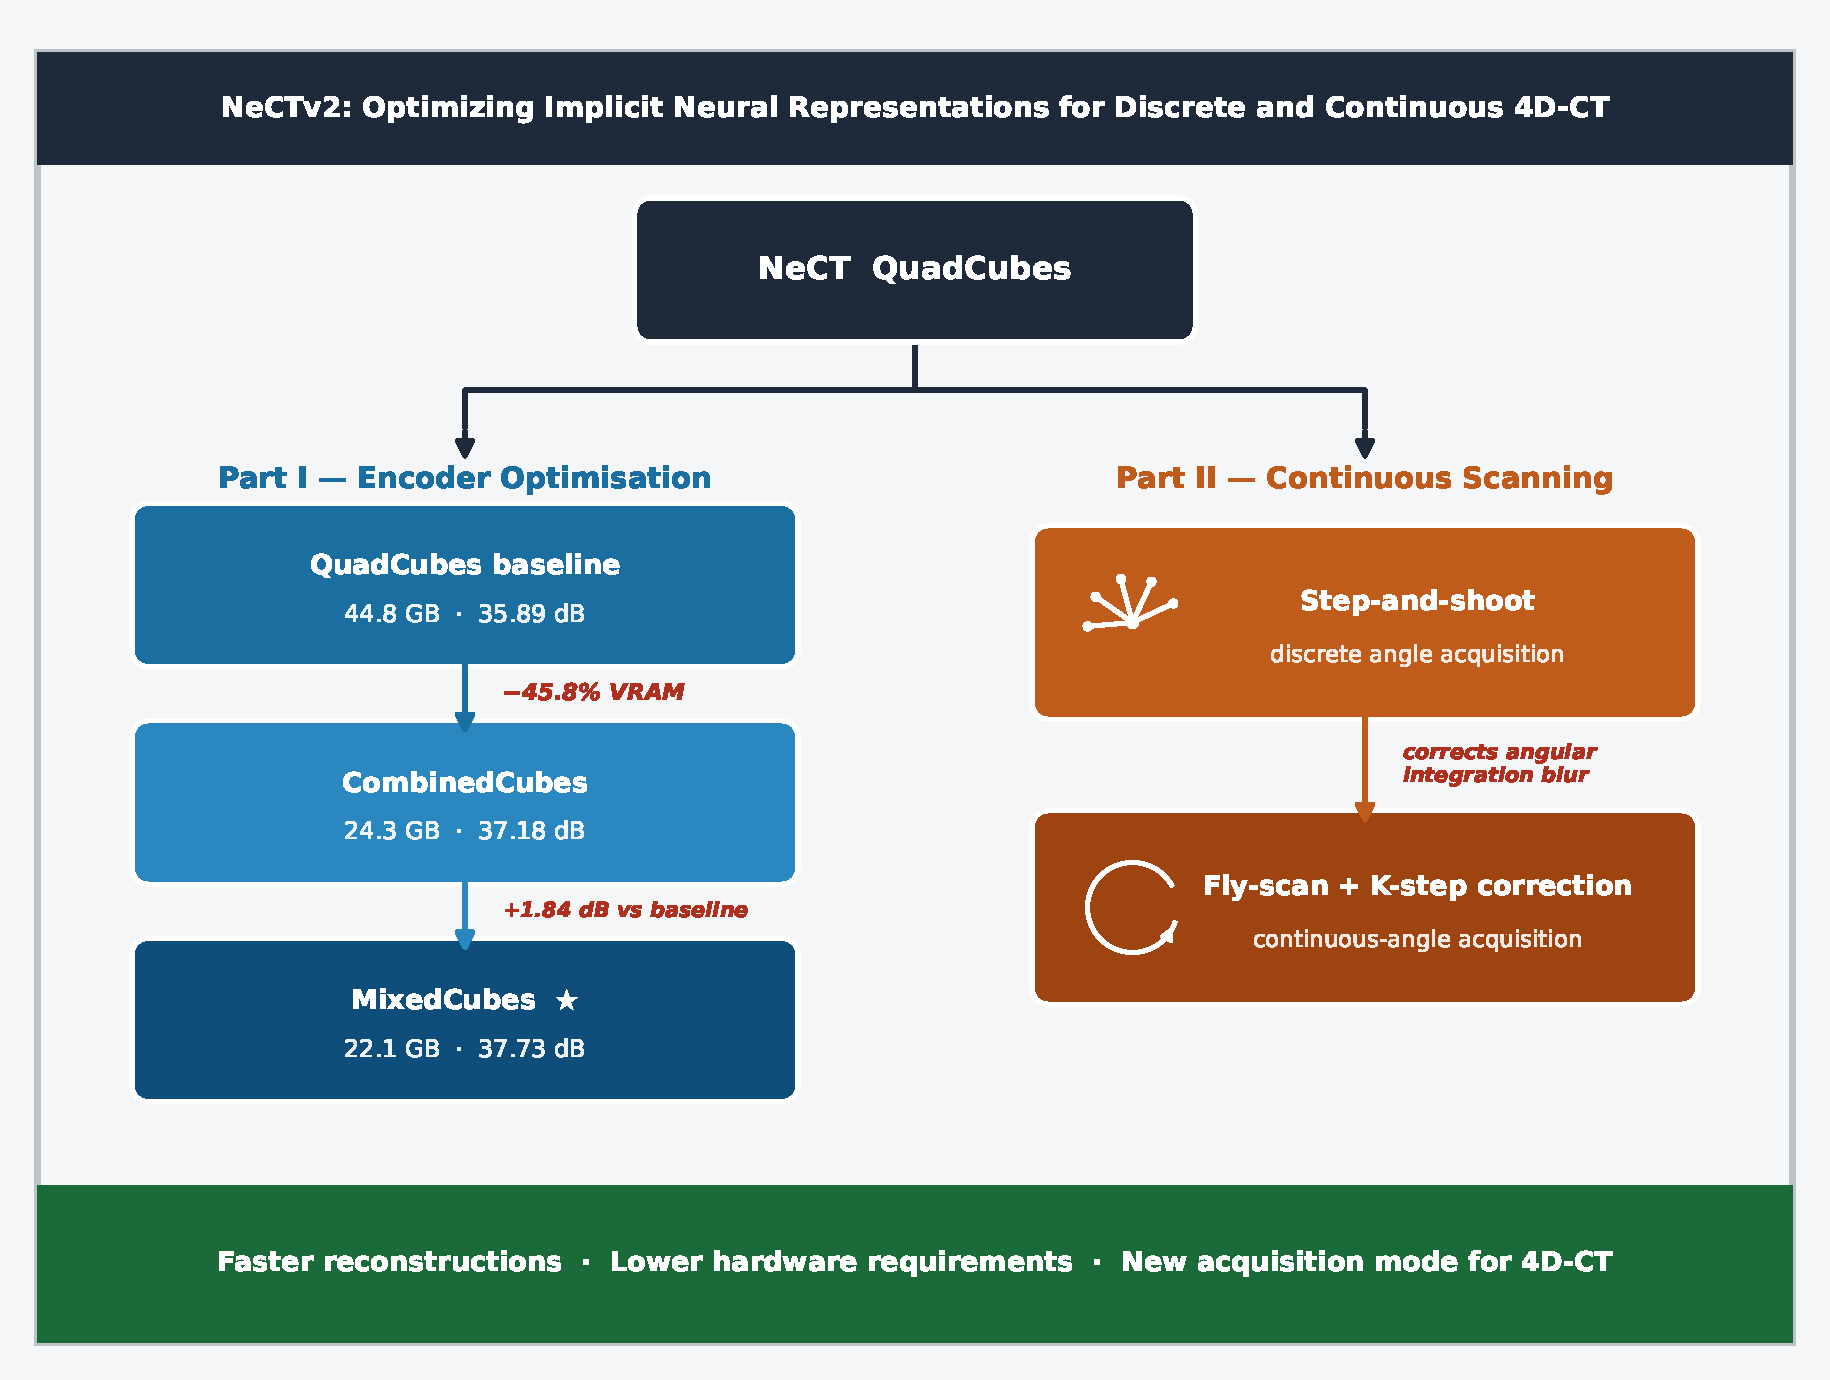
\includegraphics[width=1.4\textwidth]{thesis_overview.pdf}
    \caption{Overview of the two contributions of this thesis relative to the NeCT QuadCubes baseline (44.8\,GB, 35.89\,dB PSNR at 24\,h). Part~\ref{part:encoder_optimisation} investigates the encoder design space, with CombinedCubes reducing VRAM by 45.8\,\% (24.3\,GB) at $+1.29$\,dB and \MixedCubes{} reducing VRAM by 50.7\,\% (22.1\,GB) at $+1.84$\,dB. Part~\ref{part:continuous_scanning} extends the NeCT Beer--Lambert forward model to account for the angular integration that arises during fly-scan (continuous rotation) acquisition.}
    \label{fig:thesis_overview}
\end{figure}

% ═════════════════════════════════════════════════════════════════════════════
\part{Background}
\label{part:background}
% ═════════════════════════════════════════════════════════════════════════════
\chapter{Background}
\label{chap:background}

% ─────────────────────────────────────────────────────────────────────────────
\section{X-ray Computed Tomography}
\label{sec:ct}
% ─────────────────────────────────────────────────────────────────────────────

\subsection{Physical Principles}
\label{subsec:ct_physics}

X-ray computed tomography reconstructs the three-dimensional internal structure of an object from a set of its two-dimensional projections. The physical quantity being reconstructed is the linear attenuation coefficient $\mu(\mathbf{r})$, a material-dependent scalar field defined at every point $\mathbf{r} = (x, y, z)$ in the object that describes how strongly the local material absorbs or scatters X-ray photons. The SI unit of $\mu$ is \si{\per\metre} and it depends on both the material density and the photon energy. In attenuation-contrast CT the contrast between different materials arises entirely from differences in $\mu$.

When a monochromatic X-ray beam of initial intensity $I_0$ travels through a heterogeneous material along a straight ray path, the transmitted intensity $I$ is governed by Beer--Lambert's law:
%
\begin{equation}
    I = I_0 \exp\!\left(-\int_{\mathrm{ray}} \mu\!\left(\mathbf{r}(s)\right) \mathrm{d}s\right),
    \label{eq:beer_lambert}
\end{equation}
%
where the integral is taken along the parameterised ray path $\mathbf{r}(s) = \mathbf{o} + s\,\mathbf{d}$, with $\mathbf{o}$ the source position, $\mathbf{d}$ a unit direction vector, and $s$ the arc-length parameter along the ray. The symbol $t$ is reserved for time throughout this thesis. Taking the negative logarithm of the transmitted-to-incident intensity ratio gives the line integral of $\mu$ along the ray, also called the projection value $p$:
%
\begin{equation}
    p = -\ln\!\left(\frac{I}{I_0}\right) = \int_{\mathrm{ray}} \mu\!\left(\mathbf{r}(s)\right) \mathrm{d}s.
    \label{eq:projection_value}
\end{equation}
%
CT reconstruction is the inverse problem of recovering $\mu(\mathbf{r})$ from a finite set of such projection values. Beer--Lambert's law assumes the X-ray beam is effectively monochromatic and that scattering is negligible, both of which are standard assumptions in laboratory micro-CT analysis \citep{kak2001principles}.

In cone-beam CT (CBCT), a point X-ray source illuminates the entire sample simultaneously with a divergent cone-shaped beam. The transmitted intensities are recorded on a flat 2D area detector. This is the geometry of standard laboratory micro-CT instruments. A single projection, also called a radiograph, is the 2D image $\{I_j\}$ recorded by the detector at one angular position of the rotating sample, where $j$ indexes the detector pixels. As the sample rotates, successive projections sweep a full $360\degree$ arc, and the complete set of projections forms the sinogram.

In practice the continuous Beer--Lambert integral is approximated by a discrete sum over $K$ sample points along the ray:
%
\begin{equation}
    p_j \approx \sum_{k=1}^{K} \mu\!\left(\mathbf{r}_k\right) \Delta s,
    \label{eq:discrete_projection}
\end{equation}
%
where $\Delta s$ is the sampling step size. CT reconstruction then amounts to inverting the system of equations $\{p_j = \mathcal{A}\mu\}$, where $\mathcal{A}$ is the forward projection operator. The system is highly underdetermined when the number of projections is small relative to the number of voxels, making the inverse problem ill-posed and requiring regularisation or prior information for a stable solution.

\subsection{Classical Reconstruction Algorithms}
\label{subsec:ct_algorithms}

Reconstruction algorithms fall into two broad families. Analytical methods derive a closed-form inversion formula from the Fourier slice theorem \citep{radon1917, kak2001principles}, while iterative methods formulate reconstruction as an optimisation problem.

The Feldkamp--Davis--Kress (FDK) algorithm \citep{feldkamp1984} is the standard workhorse for cone-beam CT. It approximates the 3D cone-beam geometry by treating each detector row as an independent tilted fan-beam slice, applies a cosine-weighted ramp filter, and back-projects the filtered data into a 3D reconstruction volume. FDK is non-iterative and fast, but requires the number of projections $N_\phi$ to satisfy the Shannon--Nyquist criterion, approximately $N_\phi \geq \pi N / 2$ for $N$ pixels across the field of view \citep{kak2001principles}. When this condition is violated, as it inevitably is in sparse-view CT, reconstructions suffer from characteristic streak artefacts.

Iterative methods formulate reconstruction as minimisation of a data fidelity term. The simultaneous algebraic reconstruction technique (SART) \citep{gordon1970algebraic, andersen1984sart} updates all voxels simultaneously using rays from one projection angle at each step. Ordered subsets SART (OS-SART) further accelerates convergence by processing projections in angularly diverse subsets \citep{du2017convergence}. Adding total variation (TV) regularisation yields OS-SART-TV, which penalises the image gradient magnitude:
%
\begin{equation}
    \mathcal{R}_\mathrm{TV}(\mu) = \sum_{\mathbf{r}}
        \left\|\nabla \mu(\mathbf{r})\right\|_2,
    \label{eq:tv_regularisation}
\end{equation}
%
promoting piecewise-constant solutions. TV regularisation can suppress streak artefacts in sparse-view conditions, but introduces contrast reduction as the penalty discourages gradients everywhere, smoothing out fine features \citep{kak2001principles}.

Both FDK and OS-SART-TV were designed for static 3D CT. Neither algorithm can use information from other time steps to improve a given frame, so each reconstruction is treated independently.

\subsection{4D-CT and Dynamic Imaging}
\label{subsec:4dct}

4D-CT denotes acquisition and reconstruction of CT data from a sample that evolves over time, producing a time-resolved sequence of 3D images. In geosciences, 4D-CT is applied to study mechanical deformation of rocks, multiphase fluid flow, CO$_2$ mineralisation, and reactive dissolution \citep{withers2021ct, gan2020application}. The central challenge is achieving sufficient temporal resolution to capture the process of interest while maintaining the spatial resolution needed to observe pore-scale phenomena.

The temporal resolution of a conventional 4D-CT scan is limited by the time required to collect enough angular projections for a 3D reconstruction. In sequential scanning a full $360\degree$ rotation is completed before moving to the next time step, giving a temporal resolution on the order of one hour for laboratory micro-CT. Reducing this requires fewer projections per time step, which degrades reconstruction quality. Several mitigation strategies exist, including incorporating prior information from a high-quality static scan \citep{chen2008piccs, myers2011dynamic}, penalising the temporal derivative of $\mu$ to enforce smooth evolution \citep{goethals2022dynamic}, representing the object as a continuous function of time fit to all projections simultaneously \citep{goethals2025dyrect}, and parameterising the field as an INR as in NeCT \citep{friis2025nect}.

The photon flux of the X-ray source is a fundamental constraint. Synchrotron sources provide a beam brilliance 10--14 orders of magnitude higher than laboratory tubes \citep{withers2021ct}, enabling sub-second exposures. Standard laboratory instruments are far more accessible but require longer exposures, limiting acquisition speed.

The choice of angular sampling scheme affects how much complementary information is gathered per projection. In equiangular scanning, projections are collected at equally spaced angles, which is well suited to static reconstruction but provides redundant angular coverage in dynamic experiments where consecutive projections are taken at similar angles. The golden-angle sampling scheme sets the angular increment to $\Delta\phi \approx 137.51\degree$, distributing projections nearly optimally on a circle as more are accumulated \citep{kohler2004golden}. At any point during acquisition, the projections collected so far are as uniformly spread in angle as possible, which is useful for time-resolved imaging where the effective number of projections per time step is small.

\section{Neural Networks}
\label{sec:nn}
% ─────────────────────────────────────────────────────────────────────────────

A neural network is a parameterised function whose internal parameters are adjusted iteratively until the function approximates a desired input-output relationship. The basic computational unit is the neuron, which computes a weighted sum of its inputs and passes the result through a nonlinear activation function. By stacking many neurons into layers and connecting layers sequentially, a network can represent increasingly complex relationships between its inputs and outputs.

The fundamental architecture used throughout this work is the \emph{multilayer perceptron} (MLP), sometimes called a fully-connected or feedforward network. An MLP consists of an input layer, one or more hidden layers, and an output layer. Each layer $\ell$ applies a learned affine transformation followed by a nonlinear activation function:
%
\begin{equation}
    \mathbf{h}^{(\ell)} = \sigma\!\left( W^{(\ell)}\, \mathbf{h}^{(\ell-1)} + \mathbf{b}^{(\ell)} \right),
    \label{eq:mlp_layer}
\end{equation}
%
where $W^{(\ell)}$ is the weight matrix, $\mathbf{b}^{(\ell)}$ is the bias vector of layer $\ell$, and $\sigma$ denotes the activation function applied element-wise. The input to the first layer is the network input $\mathbf{h}^{(0)} = \mathbf{x}$, and the output of the final layer $L$ is the prediction $\hat{y} = \mathbf{h}^{(L)}$.

The composition of $L$ such layers defines a function $f_{\boldsymbol{\theta}} : \mathbb{R}^{n} \to \mathbb{R}^{m}$, where $\boldsymbol{\theta}$ collects all learnable parameters $\{W^{(\ell)}, \mathbf{b}^{(\ell)}\}_{\ell=1}^{L}$. By the universal approximation theorem, an MLP with at least one hidden layer and a nonlinear activation can approximate any continuous function on a compact domain to arbitrary precision given sufficient capacity \citep{cybenko1989approximation, hornik1989multilayer}.

Common activation functions include sigmoid $\sigma(z) = (1 + e^{-z})^{-1}$ and hyperbolic tangent $\sigma(z) = \tanh(z)$, both of which saturate for large inputs and can cause vanishing gradients in deep networks. The rectified linear unit (ReLU), $\sigma(z) = \max(0, z)$, largely solved this problem and became the default choice \citep{nair2010rectified}. A known failure mode of ReLU is that neurons whose pre-activation is consistently negative receive no gradient and become permanently inactive. The Leaky ReLU addresses this by allowing a small gradient for negative inputs:
%
\begin{equation}
    \sigma(z) = \begin{cases} z & z > 0 \\ \alpha z & z \leq 0, \end{cases}
    \label{eq:leaky_relu}
\end{equation}
%
where $\alpha \ll 1$ is a small constant. For applications requiring the network to represent signals with significant high-frequency content, periodic activations such as sinusoidal representation networks (SIREN, $\sigma(z) = \sin(z)$) have been proposed \citep{sitzmann2020siren}.

Training a network means finding the parameter vector $\boldsymbol{\theta}$ that minimises a scalar loss function $\mathcal{L}(\boldsymbol{\theta})$ measuring the discrepancy between predictions and observations. For regression tasks the two most common choices are the mean squared error (L2 loss) and the mean absolute error (L1 loss):
%
\begin{align}
    \mathcal{L}_{\mathrm{L2}} &= \frac{1}{N}\sum_{i=1}^{N}\left(\hat{y}_i - y_i\right)^2,
    \label{eq:l2_loss} \\
    \mathcal{L}_{\mathrm{L1}} &= \frac{1}{N}\sum_{i=1}^{N}\left|\hat{y}_i - y_i\right|.
    \label{eq:l1_loss}
\end{align}
%
L1 loss is less sensitive to outliers than L2 and is often preferred when the measurements contain occasional corrupted samples. Parameters are updated by gradient descent, where at each step $\boldsymbol{\theta}$ is adjusted in the direction of steepest descent of $\mathcal{L}$. The gradient $\nabla_{\boldsymbol{\theta}} \mathcal{L}$ is computed by backpropagation, which applies the chain rule layer by layer from the output back to the input \citep{rumelhart1986backprop}. In practice the gradient is estimated from a random mini-batch of $B$ data points at each step rather than from the full dataset. The Adam optimiser \citep{kingma2015adam}, which maintains per-parameter running estimates of the first and second gradient moments, is the standard choice for training coordinate networks.

\section{Convolutional Neural Networks and Image-to-Image Architectures}
\label{subsec:cnn}

While the MLP treats every input element independently, images have strong local structure. Nearby pixels tend to be similar, and the same local pattern such as an edge or a texture can appear anywhere in the image. Convolutional neural networks (CNNs) exploit this by replacing the dense weight matrices of an MLP with learned local filters that slide across the spatial extent of the input \citep{lecun1998gradient}.

A discrete 2D convolution of an input feature map $\mathbf{X} \in \mathbb{R}^{H \times W}$ with a filter $\mathbf{K} \in \mathbb{R}^{k \times k}$ produces an output feature map $\mathbf{Y}$ whose entries are
%
\begin{equation}
    Y_{i,j} = \sum_{p=0}^{k-1}\sum_{q=0}^{k-1} K_{p,q}\, X_{i+p,\, j+q}.
    \label{eq:conv2d}
\end{equation}
%
The same kernel $\mathbf{K}$ is applied at every spatial position, so the number of learnable parameters depends only on the kernel size rather than the image dimensions. Each output unit depends on only a $k \times k$ neighbourhood of the input, called its receptive field. Stacking multiple convolutional layers increases the effective receptive field of deeper units, allowing the network to integrate information across progressively larger regions. Pooling layers downsample the feature maps, introducing robustness to small spatial shifts.

\subsubsection*{Limitations for CNN- and Attention-Based Approaches}

Despite their strong empirical performance on static reconstruction tasks, CNN- and transformer-based approaches share a set of structural limitations. They must be trained on a dataset of paired examples before deployment, so assembling training data for a new experimental configuration is expensive. Once trained, the network is committed to that configuration and applying it to a new one requires retraining. These networks have no internal model of the measurement process and learn only a statistical mapping from the training distribution. When the test image differs from that distribution, as is common in novel scientific experiments, the network can produce physically incorrect features with high confidence \citep{patwari2023hallucination}. They also operate on discrete pixel or voxel grids, so the spatial resolution is fixed at training time. Representing a continuously evolving three-dimensional object at arbitrary spatial and temporal coordinates is not normally the application for these frameworks.


\section{Implicit Neural Representations}
\label{subsec:inr}

An implicit neural representation (INR) \citep{sitzmann2020siren}, sometimes called a coordinate network or neural field, is a neural network trained to represent a signal as a continuous function of its coordinates. Formally, an INR is a parameterised function
%
\begin{equation}
    f_\theta : \mathbb{R}^n \longrightarrow \mathbb{R}^m,
    \label{eq:inr_def}
\end{equation}
%
where $\boldsymbol{\theta}$ denotes the network weights, the input is a coordinate vector such as a spatial position or a position-time pair, and the output is the signal value at that coordinate. The signal is implicit in the sense that it is never stored as a discrete grid of samples. Instead, the continuous function $f_{\boldsymbol{\theta}}$ is the representation itself, and individual values are obtained by evaluating the network at any desired coordinate.

A 3D volume stored as a voxel grid of resolution $N^3$ requires memory proportional to $N^3$. An INR stores only its network weights, whose count is independent of the desired output resolution. The same network architecture can be queried at $128^3$ or $1024^3$ spatial positions without any change to its parameter count, making INRs inherently resolution-agnostic.

An INR is instance-specific, meaning it is trained from scratch for each individual signal, using only the measurements of that signal as supervision. No external datasets or prior training are needed. The optimisation proceeds by defining a differentiable forward model that maps the network's predicted field to the expected measurements, then minimising the discrepancy between those predictions and the actual observations. Because the physics of the measurement process is embedded directly in the optimisation loop, the reconstruction is constrained to be consistent with the known forward model. This prevents the generation of features that are inconsistent with the measurements, which is a significant failure mode of trained CNN approaches \citep{patwari2023hallucination}.

A naive INR, one in which an MLP receives raw coordinate inputs, struggles to represent signals with significant high-frequency content such as sharp material boundaries. This is a consequence of spectral bias, where gradient-based training causes MLPs to learn low-frequency components of a target function far faster than high-frequency ones \citep{rahaman2019spectral}. Analysed through the neural tangent kernel (NTK), a standard coordinate-based MLP corresponds to a kernel whose eigenvalue spectrum decays rapidly with frequency, which prevents convergence to high-frequency components within a practical number of optimisation steps \citep{tancik2020fourier}.

The standard remedy is to map the raw input coordinates $\mathbf{x} \in \mathbb{R}^n$ through a positional encoding $\gamma : \mathbb{R}^n \to \mathbb{R}^d$ before passing them to the MLP, where $d \gg n$:
%
\begin{equation}
    f_\theta(\mathbf{x}) = \mathrm{MLP}_\theta\!\left(\gamma(\mathbf{x})\right).
    \label{eq:inr_with_encoding}
\end{equation}
%
The sinusoidal positional encoding popularised by NeRF \citep{mildenhall2021nerf} maps each coordinate to a sequence of sines and cosines at exponentially increasing frequencies:
%
\begin{equation}
    \gamma(\mathbf{x}) = \left(
        \sin(2^0 \pi \mathbf{x}),\;
        \cos(2^0 \pi \mathbf{x}),\;
        \ldots,\;
        \sin(2^{L-1} \pi \mathbf{x}),\;
        \cos(2^{L-1} \pi \mathbf{x})
    \right),
    \label{eq:sinusoidal_encoding}
\end{equation}
%
where $L$ is the number of frequency octaves. \citet{tancik2020fourier} showed using NTK theory that this encoding transforms the effective kernel into a stationary one with a tunable bandwidth, directly addressing spectral bias. An alternative is to use random Fourier features $\gamma(\mathbf{x}) = [\sin(\mathbf{B}\mathbf{x}),\, \cos(\mathbf{B}\mathbf{x})]$, where each row of $\mathbf{B}$ is sampled from a Gaussian $\mathcal{N}(\mathbf{0}, \sigma^2 \mathbf{I})$ with bandwidth $\sigma$ chosen to match the signal's frequency content.

Both sinusoidal encodings and random Fourier features are fixed and not updated during training. A more capable alternative is to learn the encoding jointly with the MLP. The multiresolution hash encoding of \citet{mueller2022instant} pursues joint encoder and MLP training by storing trainable feature vectors in a set of hash tables indexed by the input coordinates at multiple spatial resolutions. The hash encoding shifts much of the representational work from the MLP to the encoding tables, allowing a smaller and faster MLP to achieve equal or better reconstruction quality. The hash encoding is described in detail in \cref{subsubsec:hash_encoding}.

\subsection{Neural Radiance Fields (NeRF)}
\label{subsec:nerf}

Neural Radiance Fields (NeRF), introduced by \citet{mildenhall2021nerf}, demonstrated that a complex 3D scene could be fully represented by the weights of a small MLP trained on a set of 2D photographs taken from known camera positions, and that this representation was sufficient to synthesise photorealistic images from arbitrary new viewpoints. What made NeRF influential beyond its original application was the mathematical structure it established. It consists of a differentiable forward model connecting a continuous volumetric field to 2D observations via a ray integral, trained end-to-end by minimising the discrepancy between simulated and measured projections. This same structure, a continuous scalar field recovered through a physics-based differentiable renderer, is directly applicable to tomographic reconstruction.

NeRF represents a static scene as a continuous 5D function
%
\begin{equation}
    F_\Theta : (\mathbf{x},\, \mathbf{d}) \longrightarrow (\mathbf{c},\, \sigma),
    \label{eq:nerf_fn}
\end{equation}
%
where $\mathbf{x} = (x, y, z) \in \mathbb{R}^3$ is a spatial location, $\mathbf{d} \in \mathbb{S}^2$ is a unit viewing direction, $\mathbf{c} = (r, g, b)$ is the emitted RGB colour, and $\sigma \geq 0$ is the volume density at $\mathbf{x}$. The density represents the differential probability that a ray is absorbed at $\mathbf{x}$ and is predicted from position only to enforce multi-view consistency. The colour depends on both position and direction, allowing NeRF to represent view-dependent effects such as specular reflections.

\begin{figure}[htbp]
    \centering
    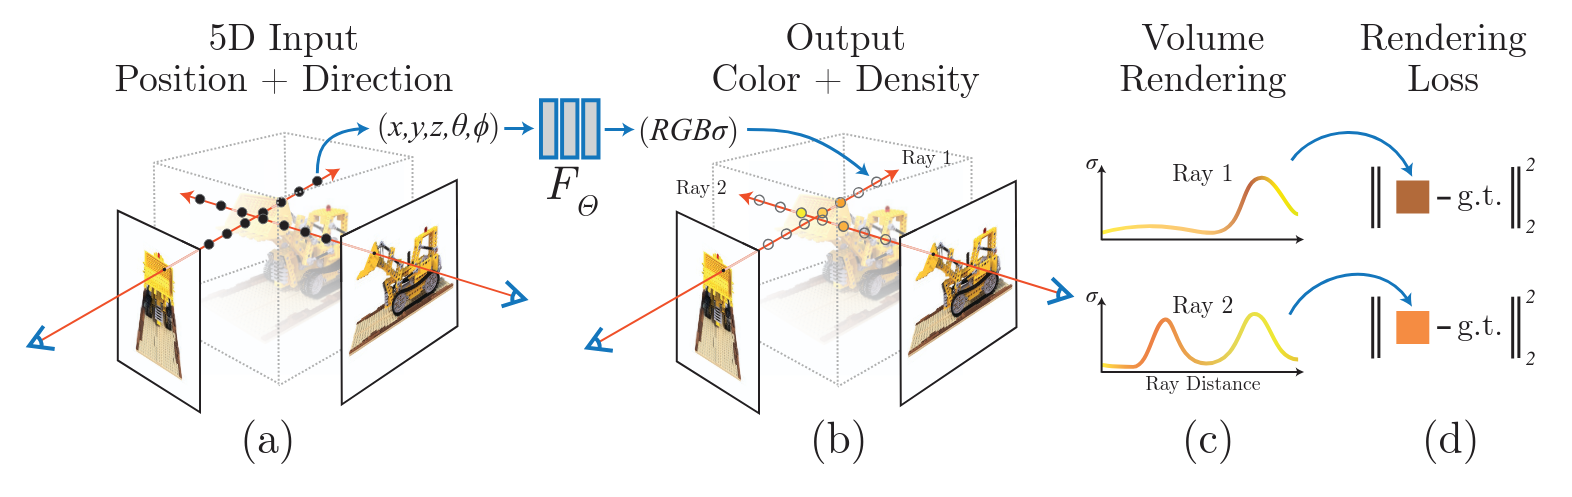
\includegraphics[width=1.0\textwidth]{nerf.png}
    \caption{The NeRF pipeline. A continuous 5D function mapping spatial position and viewing direction to colour and density is represented by an MLP. Rays are marched through the volume, and the rendered pixel colour is compared to the observed image to supervise training via backpropagation.}
    \label{fig:nerf_pipeline}
\end{figure}

To render the colour at a pixel, a camera ray $\mathbf{r}(t) = \mathbf{o} + t\mathbf{d}$ is cast from the camera origin $\mathbf{o}$ into the scene. The expected colour $C(\mathbf{r})$ accumulated along the ray between near and far bounds $t_n$ and $t_f$ is given by the volume rendering integral \citep{kajiya1984ray}:
%
\begin{equation}
    C(\mathbf{r}) = \int_{t_n}^{t_f}
        T(t)\; \sigma\!\left(\mathbf{r}(t)\right)\;
        \mathbf{c}\!\left(\mathbf{r}(t), \mathbf{d}\right) \, \mathrm{d}t,
    \label{eq:volume_rendering}
\end{equation}
%
where the accumulated transmittance $T(t) = \exp\!\left(-\int_{t_n}^{t} \sigma(\mathbf{r}(s)) \mathrm{d}s\right)$ is the probability that the ray travels from $t_n$ to $t$ without being absorbed. The integral is approximated using stratified sampling, dividing the interval $[t_n, t_f]$ into $N$ bins with one sample $t_i$ drawn uniformly from each \citep{mildenhall2021nerf}:
%
\begin{equation}
    \hat{C}(\mathbf{r}) = \sum_{i=1}^{N}
        T_i \left(1 - e^{-\sigma_i \delta_i}\right) \mathbf{c}_i,
    \qquad
    T_i = \exp\!\left(-\sum_{j=1}^{i-1} \sigma_j \delta_j\right),
    \label{eq:nerf_discrete}
\end{equation}
%
where $\delta_i = t_{i+1} - t_i$ is the distance between adjacent samples. This expression is fully differentiable with respect to the MLP parameters $\Theta$.

NeRF is trained by minimising the squared photometric error between the rendered colour and the observed pixel colour over all training rays, with no 3D supervision required. The structural parallel with CT reconstruction is close, as summarised in Table~\ref{tab:nerf_ct_analogy}. Setting $\sigma(\mathbf{x}) \equiv \mu(\mathbf{x})$ and dropping the colour output reduces the NeRF forward model to Beer--Lambert's law. The CT reconstruction problem can therefore be addressed using the same INR machinery as NeRF, substituting the Beer--Lambert integral for the volume renderer and choosing an encoding suited to the properties of tomographic data.

\begin{table}[h]
    \centering
    \caption{Structural analogy between NeRF and attenuation-contrast CT.}
    \label{tab:nerf_ct_analogy}
    \begin{tabular}{lll}
        \toprule
        \textbf{Concept} & \textbf{NeRF} & \textbf{CT} \\
        \midrule
        Recovered field    & Volume density $\sigma(\mathbf{x})$    & Attenuation coefficient $\mu(\mathbf{x})$ \\
        Measurements       & Pixel colours $C(\mathbf{r})$           & Detector intensities $I_j$               \\
        Forward model      & Volume rendering integral               & Beer--Lambert law                        \\
        Ray sampling       & Stratified random sampling              & Equidistant ray marching                 \\
        Loss function      & L2 photometric error                    & L1 intensity error                       \\
        Input encoding     & Sinusoidal $\gamma(\mathbf{x})$         & Multiresolution hash grid                \\
        \bottomrule
    \end{tabular}
\end{table}

\subsection{Multiresolution Hash Encoding}
\label{subsubsec:hash_encoding}

The sinusoidal positional encoding defined in \cref{eq:sinusoidal_encoding} resolves the spectral bias problem but places all of the representational work on the MLP. Every gradient step updates every weight in the network, and convergence is slow regardless of how well the encoding lifts the input coordinates. The multiresolution hash encoding of \citet{mueller2022instant} addresses this by distributing the work between the MLP and a set of small trainable lookup tables, allowing the MLP itself to be made much smaller. The result is a speedup of several orders of magnitude over sinusoidal-encoded NeRF at equal or better reconstruction quality \citep{mueller2022instant}.

The encoding maintains $L$ independent levels, each corresponding to a different spatial resolution. At each level $\ell$ a grid of resolution $N_\ell$ is defined, where the resolutions grow as a geometric progression between a coarsest resolution $N_\mathrm{min}$ and a finest resolution $N_\mathrm{max}$:
%
\begin{equation}
    N_\ell = \left\lfloor N_\mathrm{min} \cdot b^\ell \right\rfloor,
    \qquad
    b = \exp\!\left(\frac{\ln N_\mathrm{max} - \ln N_\mathrm{min}}{L - 1}\right).
    \label{eq:hash_resolution}
\end{equation}
%
Each level stores up to $T$ trainable feature vectors of dimension $F$, arranged in a flat array. At coarse levels, where the grid has fewer than $T$ vertices, each vertex maps to a unique array entry (a 1:1 dense mapping). At finer levels, where the number of grid vertices exceeds $T$, the array is treated as a hash table and each vertex is mapped to an entry by a spatial hash function $h : \mathbb{Z}^d \to \mathbb{Z}_T$. The total number of trainable encoding parameters is therefore bounded by $T \cdot L \cdot F$ but is typically somewhat smaller, because the coarsest levels store only as many entries as they have grid vertices rather than the full $T$.

Given an input coordinate $\mathbf{x} \in \mathbb{R}^d$, the encoding proceeds independently at each level $\ell$. The coordinate is scaled by that level's grid resolution to identify the enclosing voxel, and the $2^d$ integer corner vertices of that voxel are determined. Each corner is mapped to an array index via either the dense mapping at coarse levels or the hash function at fine levels, and the corresponding $F$-dimensional feature vectors are retrieved. These $2^d$ feature vectors are then linearly interpolated according to the fractional position of $\mathbf{x}$ within its enclosing voxel, using trilinear interpolation in 3D or the 4D analogue in space-time. The interpolated $F$-dimensional vector is the output of level $\ell$. The outputs from all $L$ levels are concatenated to form the full encoded representation $\mathbf{y} \in \mathbb{R}^{L \cdot F}$, which is then passed to the MLP:
%
\begin{equation}
\begin{aligned}
    \hat{\mu}(\mathbf{x}) &= \mathrm{MLP}_\Phi\!\left(\mathbf{y}(\mathbf{x};\, \boldsymbol{\theta})\right), \\[4pt]
    \mathbf{y}(\mathbf{x};\, \boldsymbol{\theta}) &= \left[\,
        \mathrm{interp}_0(\mathbf{x};\, \boldsymbol{\theta}_0),\;
        \mathrm{interp}_1(\mathbf{x};\, \boldsymbol{\theta}_1),\;
        \ldots,\;
        \mathrm{interp}_{L-1}(\mathbf{x};\, \boldsymbol{\theta}_{L-1})
    \,\right].
\end{aligned}
    \label{eq:hash_forward}
\end{equation}
%
Crucially, linear interpolation is differentiable, so gradients flow back through the concatenation and interpolation to the feature vectors $\boldsymbol{\theta}_\ell$ at each level, updating only the $2^d$ entries involved in each forward pass. For a 3D grid this is 8 entries per level per sample rather than every weight in the MLP. This sparse gradient update is the primary reason the encoding converges so much faster than a purely MLP-based representation \citep{mueller2022instant}.

At fine resolution levels, multiple grid vertices inevitably map to the same hash table entry. Unlike classical hash tables which resolve such collisions through chaining or probing, the multiresolution hash encoding handles them implicitly. When two vertices collide, their gradients accumulate in the same feature vector during training. The gradients from the region with the highest loss dominate the update, so the shared vector is pulled toward representing the most important detail. The MLP then uses context from the other $L - 1$ levels, which encode the same location at different resolutions with different hash functions, to disambiguate colliding entries at query time. No explicit data-structure updates such as pruning or splitting are needed at any point during training \citep{mueller2022instant}, which maps well to GPU parallelism.

Because hash table lookups are $\mathcal{O}(1)$ with no control-flow branching, all $L$ levels can be evaluated in parallel on a GPU. The small MLP that follows (see Figure~\ref{fig:static_nect} for the static architecture and Figure~\ref{fig:quadcubes_architecture} for the dynamic QuadCubes architecture) requires far fewer floating-point operations than the large MLP needed by sinusoidal encodings. Together these properties enable training to convergence in seconds rather than hours on a single GPU, a speedup of roughly two to three orders of magnitude over the original NeRF implementation \citep{mueller2022instant}.

The first application of multiresolution hash encoding to CT reconstruction was Neural Attenuation Fields (NAF) by \citet{zha2022naf}. Earlier INR-based approaches to CT, such as NeRP \citep{shen2022nerp}, used sinusoidal encodings rather than hash grids and required a high-quality prior scan for regularisation. NAF parameterises the 3D attenuation coefficient field $\mu(\mathbf{x})$ as a hash-encoded MLP and trains the network by minimising the discrepancy between simulated and measured cone-beam projections using Beer--Lambert's law as the forward model, with no external training data required. NAF outperforms both sinusoidal-encoded INRs and iterative algorithms at a fraction of the computational cost \citep{zha2022naf}.

% ─────────────────────────────────────────────────────────────────────────────
\section{NeCT: Neural Computed Tomography}
\label{sec:nect}
% ─────────────────────────────────────────────────────────────────────────────

\NeCT{} (Neural Computed Tomography) \citep{friis2025nect} is, to the best of our knowledge, the first fully INR-based algorithm for holistic time-resolved 4D-CT reconstruction. It unifies the physical forward model of cone-beam CT with the representational power of hash-encoded implicit neural representations, treating the entire dynamic experiment, all projections from all time steps, as a single joint optimisation problem. The output is a continuous function $\muhat(\mathbf{r}, t)$, the estimated attenuation coefficient at any spatial coordinate $\mathbf{r}$ and any time $t$ within the duration of the scan, from which volumetric images at arbitrary time points can be decoded by a forward pass through the network (Figure~\ref{fig:nect_pipeline}).

\NeCT{} consists of two architecturally related but distinct models. A static 3D model for sparse-view single-frame CT reconstruction serves as the spatial backbone, and a dynamic 4D model called \emph{NeCT QuadCubes} extends the static approach to time-resolved reconstruction. Both share the same training loop and loss function, differing in the structure of the hash encoding and whether the time coordinate $t$ is included as an input.

\subsection{NeCT Pipeline Overview}
\label{subsec:nect_pipeline}

\begin{figure}[htbp]
    \centering
    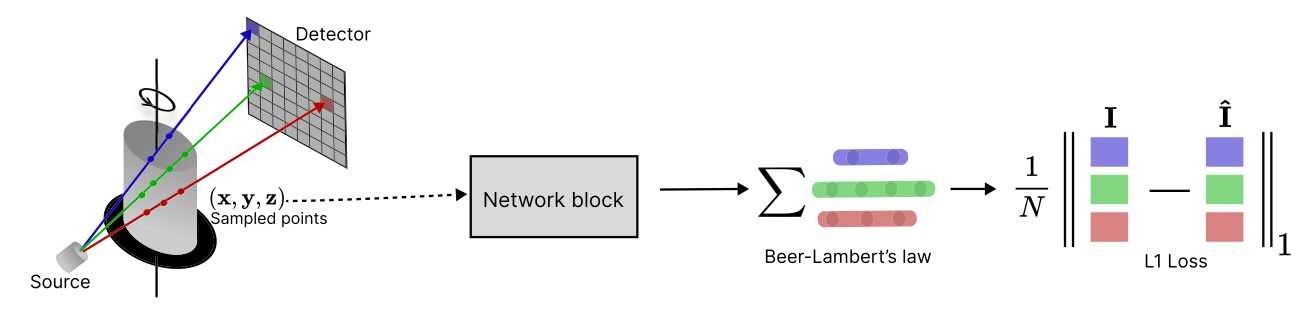
\includegraphics[width=1.0\textwidth]{nect_pipeline.png}
    \caption{The NeCT training pipeline. Rays are sampled from recorded projections, marched through the hash-encoded network to predict attenuation values, integrated via the discretised Beer--Lambert law to produce predicted detector intensities, and compared to the measured intensities by the L1 loss. Gradients are backpropagated to update the network weights.}
    \label{fig:nect_pipeline}
\end{figure}

The NeCT pipeline operates as a differentiable physics simulation. It takes the measured detector images as supervision and adjusts the network weights until the network's predictions are consistent with every recorded projection. The same four-step loop repeats for every training batch.

At each training step, a batch of $B$ rays is sampled from the full set of recorded projections. Each ray $\mathbf{r}_j(s) = \mathbf{o}_j + s\,\mathbf{d}_j$ is defined by its source position $\mathbf{o}_j$ and unit direction $\mathbf{d}_j$, determined by the cone-beam geometry of the instrument and the angular position of the projection from which the ray originates. In the dynamic model, each ray also carries a timestamp $t_j$ corresponding to the acquisition time of its projection. The measured intensity $I_j$ at the corresponding detector pixel is retrieved as the supervision target.

Each ray is then marched through the object volume by sampling $K$ equidistant points $\{\mathbf{r}_k\}_{k=1}^{K}$ along the ray within the sample bounding volume. NeCT uses an adaptive scheme in which $K$ increases linearly from $K_\mathrm{init} = 100$ to $K_\mathrm{max} = 1.5 \times \max(N_\mathrm{detector})$ over the first $30\%$ of training, where $\max(N_\mathrm{detector})$ is the number of pixels along the longest detector axis \citep{friis2025nect}. Starting with fewer points reduces computational cost in the early stages when the network is still poorly initialised, and progressively increasing the count ensures the final reconstruction is sampled finely enough to resolve sub-voxel features.

Each sampled point $(\mathbf{r}_k, t_j)$ is passed through the neural network to obtain the predicted attenuation coefficient $\muhat(\mathbf{r}_k, t_j)$. In the static model $t_j$ is omitted. The predicted detector intensity for ray $j$ is then computed by discretising Beer--Lambert's law:
%
\begin{equation}
    \hat{I}_j = I_0 \exp\!\left(-\sum_{k=1}^{K} \muhat\!\left(\mathbf{r}_k,\, t_j\right) \Delta s\right),
    \label{eq:nect_forward}
\end{equation}
%
where $\Delta s$ is the step size between adjacent sample points. The predicted intensities are compared to the measured intensities using the L1 loss over the batch:
%
\begin{equation}
    \mathcal{L} = \frac{1}{B}\sum_{j=1}^{B} \left|\hat{I}_j - I_j\right|.
    \label{eq:nect_loss}
\end{equation}
%
Gradients of $\mathcal{L}$ with respect to all network parameters are computed by automatic differentiation and used to update the parameters via the Adam optimiser \citep{kingma2015adam}. The learning rate follows a schedule with a linear warm-up over the first 5\,000 batches, after which it decays according to a cosine schedule to $1\%$ of its peak value \citep{friis2025nect}. Base learning rates are $1 \times 10^{-3}$ for static reconstructions and $2 \times 10^{-4}$ for dynamic reconstructions. The batch size is $5 \times 10^6$ ray sample points per step.

Because the hash table entries are updated only for the small subset of grid vertices intersected by each batch of rays (just $2^3 = 8$ entries per level per ray for a 3D encoder), the effective gradient update is extremely sparse, which gives the hash encoding its computational efficiency.

\subsection{Static 3D Reconstruction}
\label{subsec:nect_static}

\begin{figure}[htbp]
    \centering
    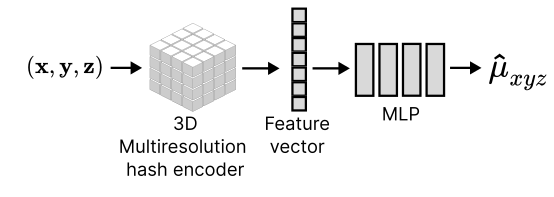
\includegraphics[width=0.80\textwidth]{static_nect.png}
    \caption{Network block for static reconstruction model using one encoder and MLP.}
    \label{fig:static_nect}
\end{figure}

The static \NeCT{} model represents the attenuation coefficient as a continuous function of spatial coordinates only, $\muhat : \mathbb{R}^3 \to \mathbb{R}$, implemented as a hash-encoded MLP (Figure~\ref{fig:static_nect}). It is architecturally derived from NAF \citep{zha2022naf} with a refined encoder configuration and training protocol.

The input spatial coordinate $\mathbf{r} = (x, y, z)$ is passed through a single 3D multiresolution hash encoder. The encoder uses a hashmap with $T = 2^{23}$ entries, $L = 23$ resolution levels, a base resolution of $N_\mathrm{min} = 16$, a growth factor of $b = 2$, and $F = 4$ features per entry \citep{friis2025nect}. The MLP has 4 hidden layers each with 128 neurons and Leaky ReLU activations, with a single linear output neuron producing the scalar $\muhat(\mathbf{r})$. The finest grid resolution $N_\mathrm{max}$ is calibrated to the detector resolution of the specific CT scan so that the finest hash grid voxels correspond approximately to the physical voxel size.

NeCT was benchmarked using peak signal-to-noise ratio (PSNR) and the structural similarity index measure (SSIM) \citep{wang2004ssim} on eleven standard 3D CT datasets from the Open SciVis Datasets project \citep{klacansky2017openscivis}. PSNR is defined as:
%
\begin{equation}
    \mathrm{PSNR} = 10 \log_{10}\!\left(\frac{R^2}{\mathrm{MSE}(\hat{\mu},\, \mu^*)}\right),
    \label{eq:psnr}
\end{equation}
%
measured in decibels, where $R$ is the dynamic range of the attenuation values. SSIM captures perceptual similarity by comparing local statistics of luminance, contrast, and structure, ranging from 0 to 1 \citep{wang2004ssim}.

NeCT outperformed FDK, OS-SART-TV, and NAF on both metrics across all eleven datasets \citep{friis2025nect}. On the Stagbeetle dataset, NeCT achieved a PSNR of 45.6\,dB and SSIM of 0.996, compared to 44.3\,dB / 0.994 for NAF, 41.9\,dB / 0.990 for OS-SART-TV, and 28.6\,dB / 0.577 for FDK. Visually, NeCT reconstructions are free of streak artefacts and show sharp material boundaries, attributed in part to the spectral regularisation effect of the hash-encoded INR \citep{friis2025nect}.

\subsection{Dynamic 4D Reconstruction: NeCT QuadCubes}
\label{subsec:nect_quadcubes}

\begin{figure}[htbp]
    \centering
    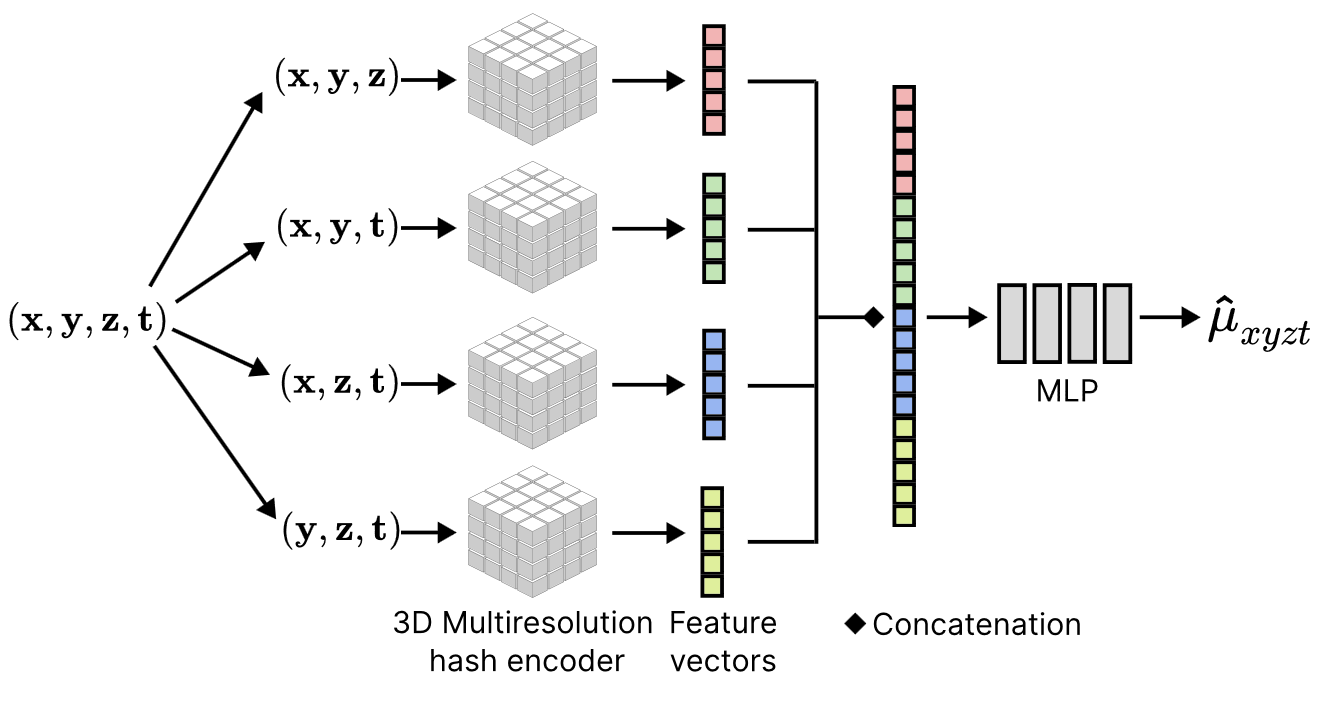
\includegraphics[width=0.95\textwidth]{quadcubes.png}
    \caption{The NeCT QuadCubes architecture. Four independent 3D multiresolution hash encoders concatenating the feature vectors are decoded by a shared MLP.}
    \label{fig:quadcubes_architecture}
\end{figure}

The dynamic NeCT model, named QuadCubes, extends the 3D INR to four dimensions by representing the attenuation field as a continuous function of both space and time, $\muhat : \mathbb{R}^3 \times \mathbb{R} \to \mathbb{R}$ (Figure~\ref{fig:quadcubes_architecture}). The central design challenge is how to structure the hash encoding for a 4D input space. QuadCubes uses four independent 3D multiresolution hash encoders, each covering a different triplet of the four space-time dimensions:
%
\begin{equation}
    \text{Encoder 1: } (x, y, z), \quad
    \text{Encoder 2: } (x, y, t), \quad
    \text{Encoder 3: } (x, z, t), \quad
    \text{Encoder 4: } (y, z, t).
    \label{eq:quadcubes_encoders}
\end{equation}
%
This set covers all four possible 3-element subsets of $\{x, y, z, t\}$, so every pair of coordinates appears together in at least two encoders. Each encoder independently produces a feature vector of dimension $L \cdot F$, and the four vectors are concatenated to form the full MLP input:
%
\begin{equation}
    \muhat(\mathbf{r}, t) = \mathrm{MLP}_\Phi\!\Bigl(
        \bigl[
            \gamma_{xyz}(\mathbf{r};\,\theta_1),\;
            \gamma_{xyt}(x,y,t;\,\theta_2),\;
            \gamma_{xzt}(x,z,t;\,\theta_3),\;
            \gamma_{yzt}(y,z,t;\,\theta_4)
        \bigr]
    \Bigr),
    \label{eq:quadcubes_forward}
\end{equation}
%
where $\gamma_{(\cdot)}$ denotes the trilinear-interpolated hash encoding in the indicated coordinate triplet and $\boldsymbol{\theta}_i$ are the trainable feature vectors of encoder $i$. The MLP has the same architecture as the static model, with 4 hidden layers of 128 neurons and Leaky ReLU activations.

Each encoder operates in a well-conditioned 3D hash space where the collision rate remains manageable at micro-CT resolutions. The overlap between encoders, where the spatial encoder \texttt{xyz} shares each of its three dimensions with one of the temporal encoders, provides redundant representations of spatial structure that assist collision disambiguation and give the MLP multiple views of the same location at different times. The rationale behind this particular factorisation, and how it compares to alternative designs, is the subject of Chapter~\ref{chap:encoder_design}.

A defining property of the QuadCubes model is that it is trained on all projections from the full dynamic experiment simultaneously. The network learns to distinguish between time-invariant structural features, which are supported by projections from all angles and all times, and dynamic features such as advancing fluid fronts, which are supported only by projections in their temporal vicinity. Static structures therefore converge to a sharp representation, while dynamic features converge with precision proportional to the rate at which they evolve relative to the projection acquisition rate. The temporal resolution is consequently scene-dependent, and for large, rapidly changing features a temporal resolution approaching the time between two successive projections is achievable \citep{friis2025nect}.

Simulations using synthetic 4D datasets generated with PoreSpy \citep{gostick2019porespy} showed that QuadCubes can resolve dynamics lasting as few as two projection intervals for large features, and approaches full resolution for events spanning ten or more projections. In the experimental Bentheimer sandstone dataset \citep{peksa2015bentheimer}, individual pore-filling events with a characteristic time of approximately 10\,s and salt dissolution events lasting approximately 30\,s were directly observed \citep{friis2025nect}.

\subsection{Hybrid Golden-Section Sampling}
\label{subsec:hybrid_golden}

\begin{figure}[htbp]
    \begin{adjustwidth}{-1.5cm}{0cm}
    \centering
    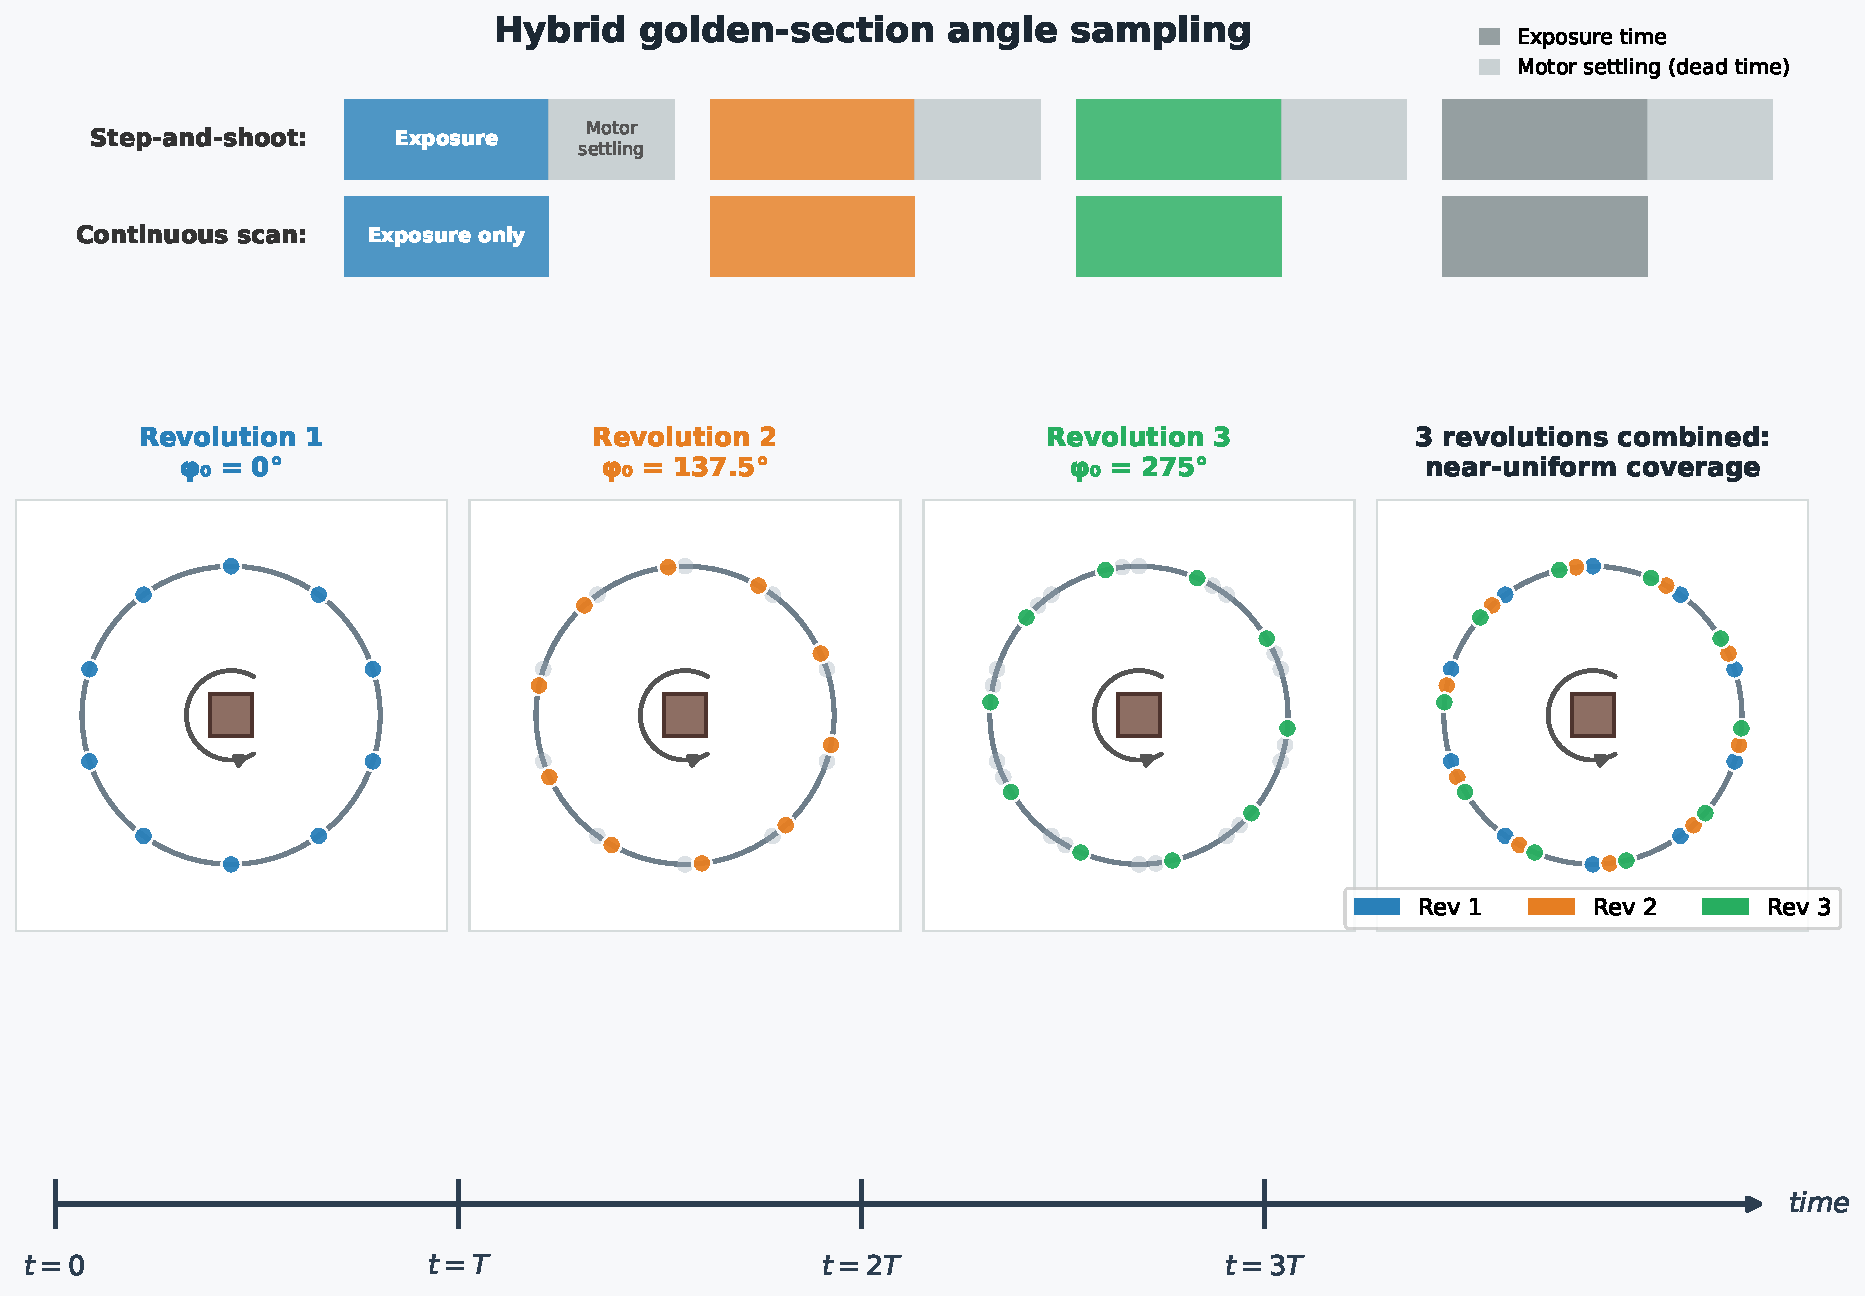
\includegraphics[width=1.3\textwidth]{fig_golden_section.pdf}
    \end{adjustwidth}
    \caption{Hybrid golden-section angle sampling illustrated across three revolutions. Each circular panel shows a top-down view of one full $360\degree$ revolution, with dots marking the angular positions of projections. Revolution~1 collects 10 equidistant projections starting at $0\degree$. Each subsequent revolution begins at a golden-angle offset ($\varphi_0 \approx 137.5\degree$), so new projections land in the largest remaining gaps. The rightmost panel shows all 30 projections combined: the coverage is nearly uniform. The timing strip at the top contrasts step-and-shoot acquisition (dead time for motor settling between exposures) with continuous rotation (full revolution time devoted to exposure). This figure is schematic; in practice 100 projections are collected per revolution.}
    \label{fig:golden_section}
\end{figure}

A practical limitation of the pure golden-angle scheme described in \cref{subsec:4dct} is that consecutive projections are separated by $137.51\degree$, requiring the sample stage to travel through a large angle between exposures. During this motor movement no projections are collected, so a significant fraction of the total scan time contributes no measurement information. The hybrid golden-section scheme, introduced by \citet{friis2025nect}, addresses this. Within each full $360\degree$ revolution a fixed number of equidistant projections are collected, but the starting angle of each revolution is offset from the previous one by the golden angle. This preserves rapid continuous rotation within each revolution while ensuring that successive revolutions are angularly offset, so that projections from different time points together cover the angular space as uniformly as possible.

This scheme provides progressive angular completeness, meaning that at any point in the experiment the projections collected so far are nearly optimally distributed in angle. For the spatial encoder \texttt{xyz}, this ensures gradient updates arrive from many different projection directions simultaneously rather than from a narrow angular range. For the temporal encoders, the golden offset means each new revolution contributes projections at angles that are maximally distinct from those of all previous revolutions, allowing the model to distinguish the attenuation field at one time from the field at neighbouring times.

In the Bentheimer sandstone experiment, 1\,400 projections were distributed across 14 revolutions of 100 projections each, with the golden offset applied between revolutions and alternating rotation direction to avoid tangling the inlet supply lines \citep{friis2025nect}. The entire 40-minute imbibition experiment was represented by a single QuadCubes model, decoded at arbitrary times to produce a continuous 3D movie of the brine invasion process.

% ═════════════════════════════════════════════════════════════════════════════

\part{Encoder Optimisation}
\label{part:encoder_optimisation}
% ═════════════════════════════════════════════════════════════════════════════

The NeCT QuadCubes architecture encodes a four-dimensional attenuation field using a set of multiresolution hash grids. In the original paper, the encoder was fixed at the largest practically feasible configuration, with neither its structural design nor its capacity optimised for training time or VRAM consumption. This part investigates both, with the goal of identifying the architecture and parameter settings that substantially reduce training time and memory footprint while preserving reconstruction quality.

Our investigation is structured around the following three governing phenomena.

First, we vary the hash collision rate, which is controlled primarily by the hashmap size and increases with encoder dimensionality. The collision rate sets the ceiling on reconstruction quality per model parameter and is the dominant driver of model size (Figure~\ref{fig:phenomena_collision}).

Second, we vary the number of resolution levels, which controls the frequency range the encoder covers simultaneously and determines, primarily, how fast the model converges within a fixed wall-clock budget. Levels have a much smaller effect on memory than on per-epoch computation time, making $L$ the primary lever for trading training speed against frequency coverage (Figure~\ref{fig:phenomena_freq}).

Third, we study asymmetric NeCT architectures that reflect the different roles of the spatial and temporal coordinates. An asymmetry between the spatial and temporal components means that the best encoder allocates capacity unequally, with consequences both for how parameters are distributed within a fixed architecture and for what the right architecture is in the first place (Figure~\ref{fig:phenomena_asymmetry}).

\begin{figure}[htbp]
    \hspace*{-2cm}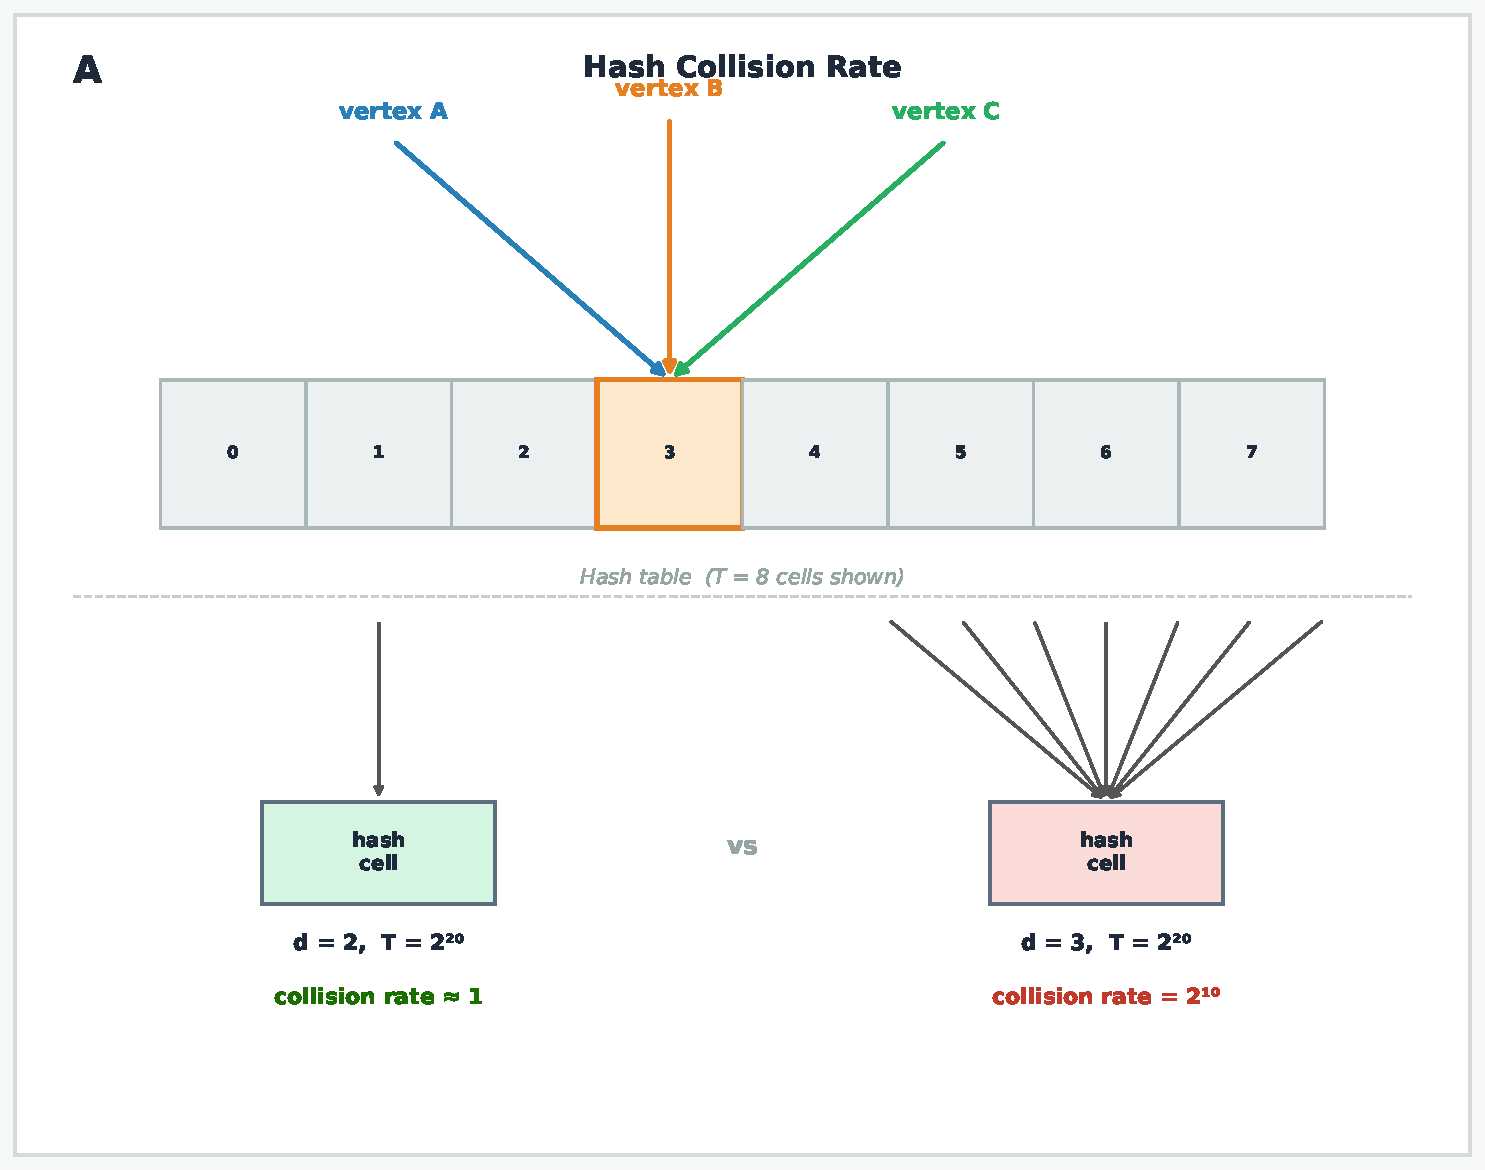
\includegraphics[width=1.3\textwidth]{fig_phenomena_A.pdf}
    \caption{\textbf{Panel A --- Hash collision rate.} When more grid vertices than hash-table entries exist at the finest level, multiple vertices must share a single stored feature vector, degrading reconstruction quality. A 2D encoder ($d=2$) at $\log_2 T = 20$ achieves near-collision-free mapping at $N_\mathrm{max} = 1024$. The same table applied to a 3D encoder ($d=3$) produces approximately $2^{10}$ vertices per entry at the finest level. Increasing $T$ reduces collisions but scales memory proportionally. The role of the finest level is further illustrated in Figure~\ref{fig:phenomena_freq}.}
    \label{fig:phenomena_collision}
\end{figure}

\begin{figure}[htbp]
    \hspace*{-2.5cm}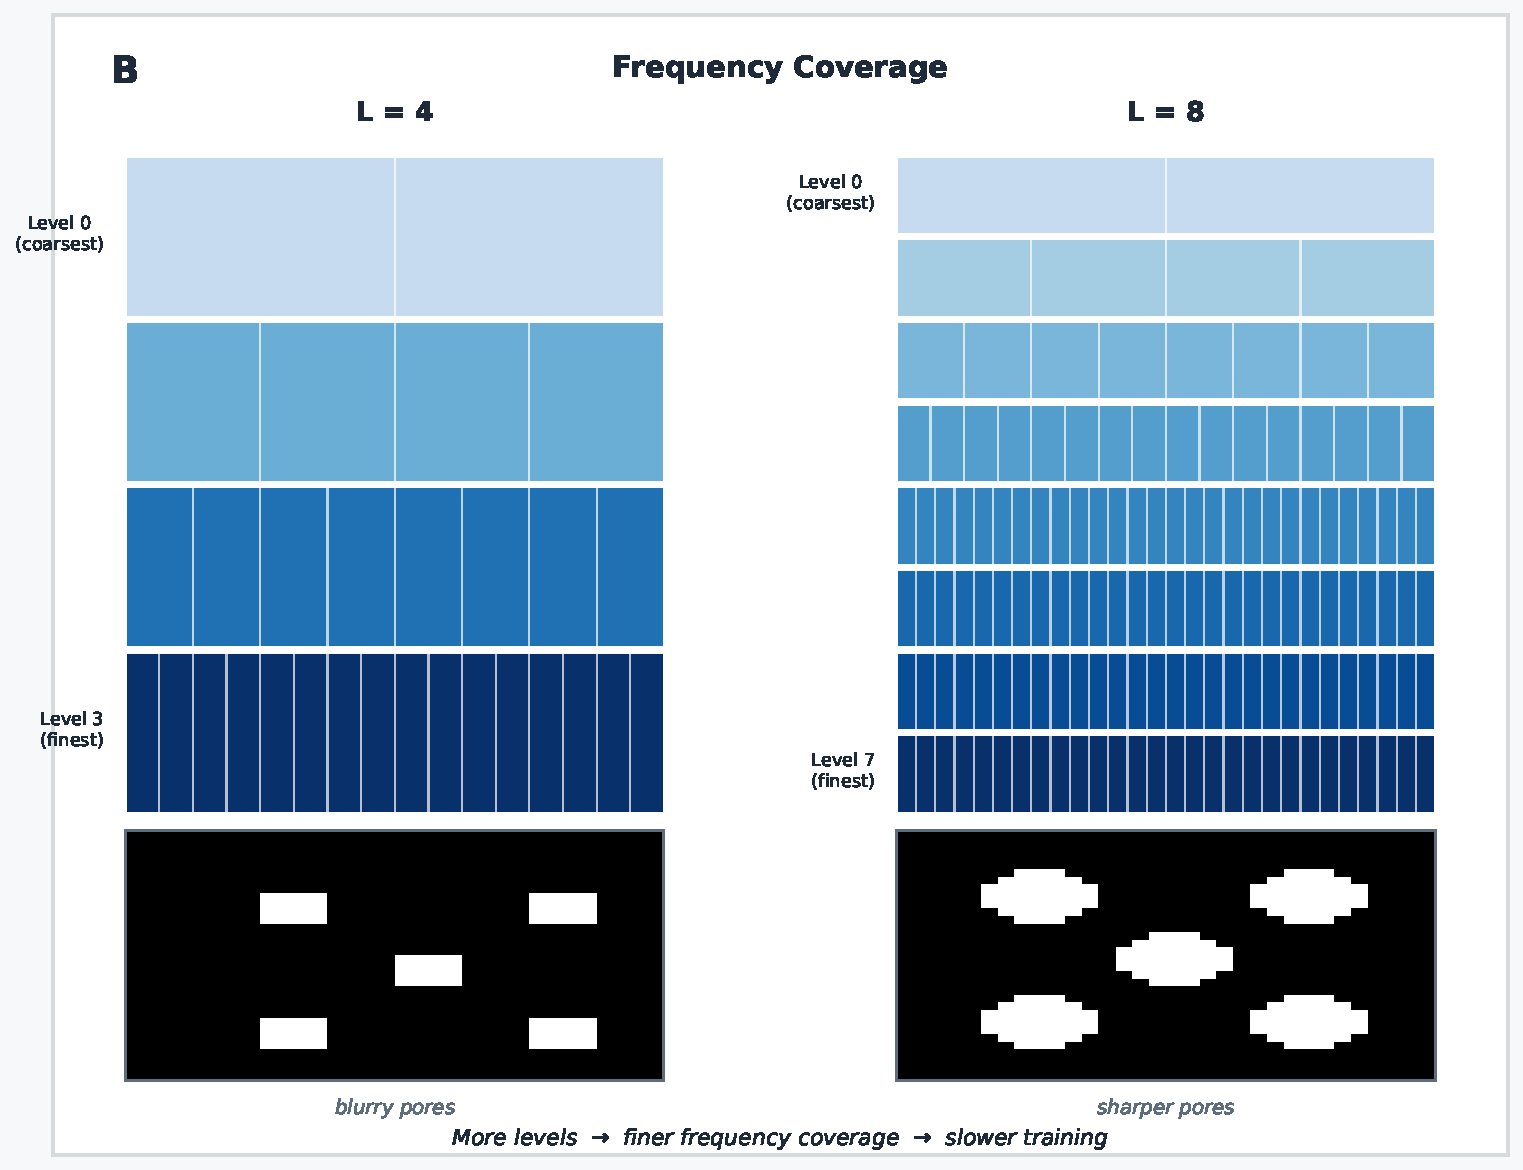
\includegraphics[width=1.3\textwidth]{fig_phenomena_B.pdf}
    \caption{\textbf{Panel B --- Resolution levels and frequency coverage.} Each level of the multiresolution hash encoding captures a distinct spatial frequency band, from coarse global structure at level 0 to fine local detail at level $L-1$. Increasing $L$ extends coverage to higher frequencies and improves asymptotic reconstruction quality, but adds one extra hash-table lookup and interpolation per sample point per training step. The dominant effect of $L$ is on per-epoch training time rather than model size.}
    \label{fig:phenomena_freq}
\end{figure}

\begin{figure}[htbp]
    \hspace*{-2cm}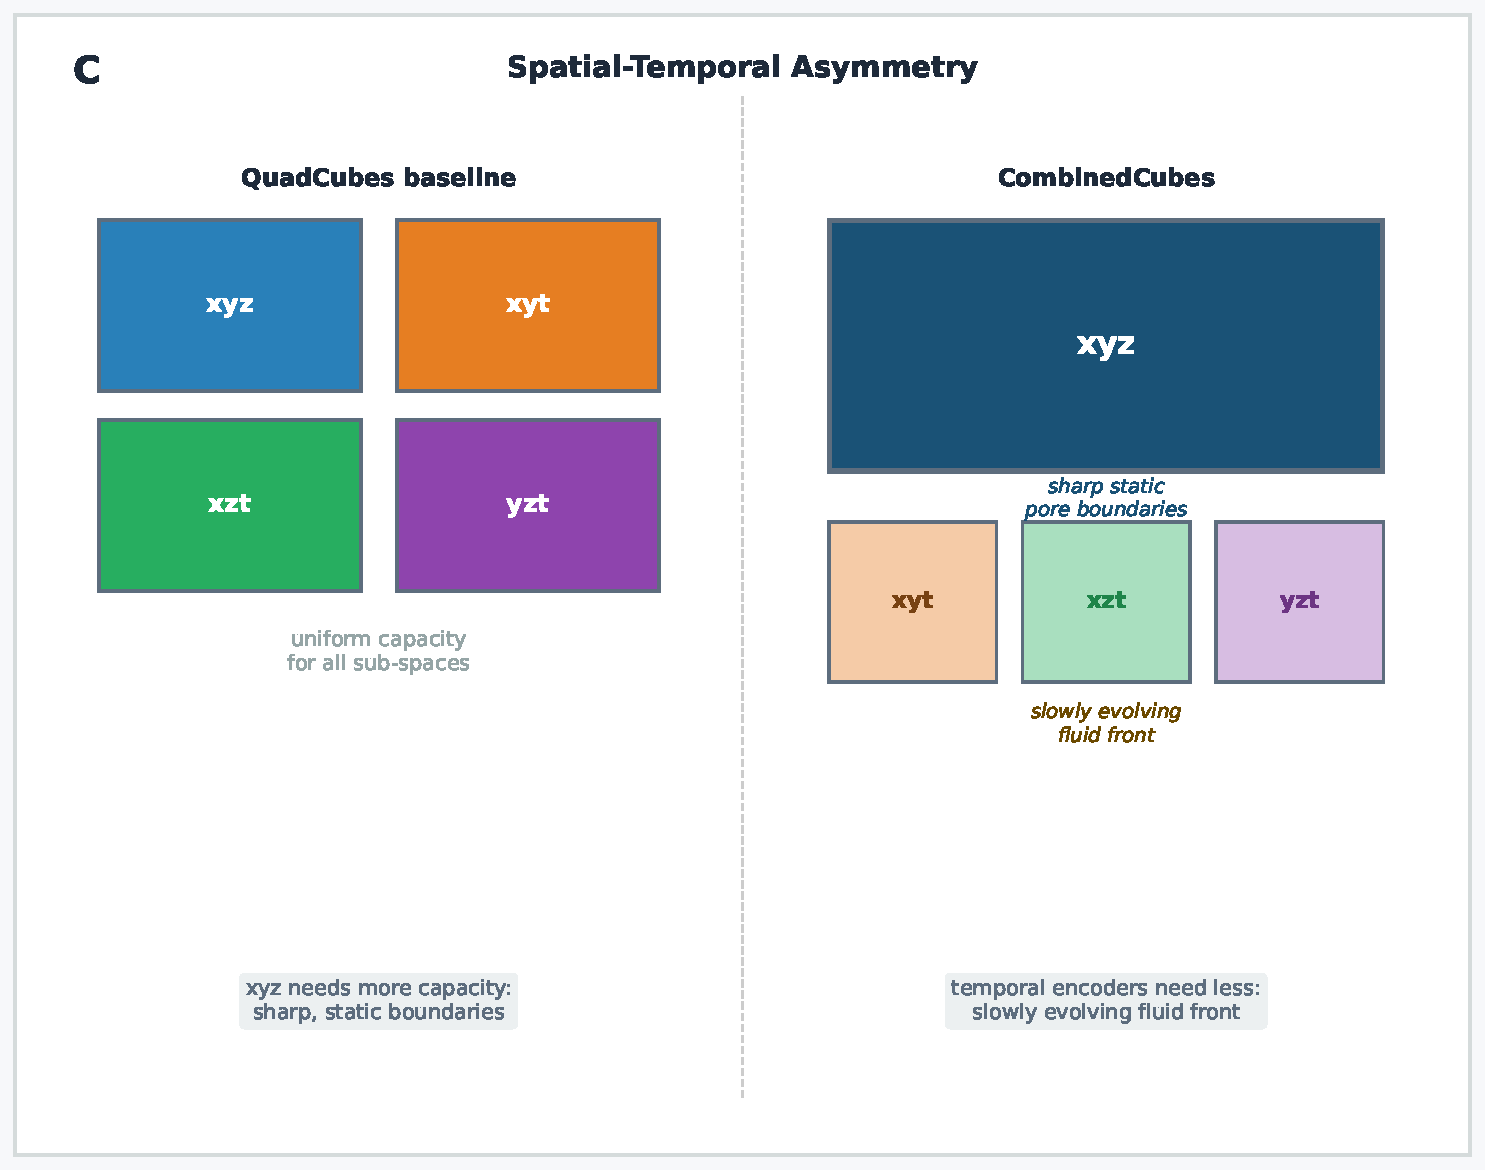
\includegraphics[width=1.3\textwidth]{fig_phenomena_C.pdf}
    \caption{\textbf{Panel C --- Spatial-temporal asymmetry.} The QuadCubes baseline assigns equal hashmap capacity to all four encoders. The $\texttt{xyz}$-encoder must represent the full high-frequency spatial structure of the pore geometry; the three temporal encoders need only track a lower-frequency signal along two spatial dimensions at a time. CombinedCubes corrects this imbalance by assigning a large 3D hash encoder to $\texttt{xyz}$ and small collision-free 2D encoders to the temporal pairs, reducing memory while improving reconstruction quality.}
    \label{fig:phenomena_asymmetry}
\end{figure}

Chapter~\ref{chap:encoder_design} works through these three phenomena in sequence. For each, the chapter first characterises it quantitatively through a systematic parameter sweep within the NeCT QuadCubes architecture, then examines an alternative architecture that either pushes the phenomenon to a catastrophic extreme, exposing the cost of getting it wrong, or addresses it effectively. Hashmap size and collision rate are paired with SingleCube. Level count and coordinate coupling are paired with the HexCubes family. The spatial-temporal capacity asymmetry is paired with CombinedCubes. Chapter~\ref{chap:encoder_comparison} places all findings into a head-to-head comparison against the QuadCubes baseline.

% ═════════════════════════════════════════════════════════════════════════════
\chapter{Encoder Design}
\label{chap:encoder_design}
% ═════════════════════════════════════════════════════════════════════════════

This chapter investigates two interrelated questions about the NeCT encoder that the original paper left unaddressed. The first is whether the QuadCubes structural decomposition of the 4D space is optimal, and the second is whether the capacity assigned to each encoder is appropriate. These questions are explored in sequence, each building on the previous finding. The chapter is organised around three sections corresponding to the three governing phenomena, covered in \cref{sec:collision_and_dim} for collision rate and hashmap size, \cref{sec:levels_and_coupling} for level count and coordinate coupling, and \cref{sec:spatial_temporal_asym} for the spatial-temporal capacity asymmetry. Each section opens with a quantitative characterisation of the phenomenon within QuadCubes and then examines the architecture that makes its consequences most visible.

% ─────────────────────────────────────────────────────────────────────────────
\section{Theory of Multiresolution Hash Encoders}
\label{sec:enc_theory}
% ─────────────────────────────────────────────────────────────────────────────

\subsection{Capacity Parameters}
\label{subsec:enc_params_theory}

The multiresolution hash encoder has three capacity parameters, the log$_2$ hashmap size ($\log_2 T$), the number of levels ($L$), and the number of features per level ($F$). These parameters are independent in the sense that each can be varied while holding the others fixed, but they affect different quantities in ways that make their roles qualitatively distinct.

The \textbf{hashmap size} $T = 2^{\log_2 T}$ is the number of feature vectors stored per level in the hash table. Because each of the $L$ levels stores at most $T$ vectors of dimension $F$, the total parameter count of the encoder is bounded by $T \cdot L \cdot F$, with $T$ entering linearly. At practical grid resolutions the finest levels have far more grid vertices than $T$ entries, so multiple vertices are mapped to the same stored vector, causing a collision. The collision rate at the finest level is approximately $N_\mathrm{max}^d / T$, where $d$ is the encoder input dimension. A higher $T$ reduces this ratio, which reduces the number of distinct spatial locations sharing each feature vector and therefore increases the representational precision available at fine scales. Hashmap size is thus the primary driver of both model size and reconstruction quality, as it controls the ceiling of spatial precision the encoder can achieve, and each doubling of $T$ roughly doubles both memory and quality headroom.

The \textbf{number of levels} $L$ determines how many spatial resolutions the encoder simultaneously represents, ranging from a coarse grid at level 0 to the finest grid at level $L-1$. Each additional level extends the encoder's coverage to a new frequency band and adds a constant forward-pass overhead, as the encoder must look up and interpolate feature vectors in one more hash table per sample point per training step. The memory contribution of additional levels is small at the coarse end (those levels are dense and have few vertices) and modest at the fine end (they are already using the full hash table). The dominant effect of $L$ is therefore on training time, as more levels means more table lookups and more MLP input dimensions, which directly increases the per-step computation without a commensurate increase in memory. Reducing $L$ saves training time at the cost of reducing the frequency range the encoder can cover.

The \textbf{features per level} $F$ sets the dimensionality of each stored and interpolated feature vector. It scales the encoder's expressivity at every spatial location and frequency simultaneously. Unlike $T$ which affects precision by reducing collision load, and unlike $L$ which extends frequency coverage, $F$ controls how much information the encoder can pack into a single spatial location at a given resolution. It also scales the input dimension of the MLP, as for QuadCubes the MLP receives a concatenated vector of $4 \cdot L \cdot F$ features. $F$ therefore affects both encoder memory (linearly) and MLP cost, making it a less independently tunable parameter than $T$ or $L$.

The MLP decoder is negligible relative to the encoders by every measure. With 4 hidden layers of 128 neurons and a concatenated input of $4 \times L \times F$ features, the baseline MLP has approximately $97\,000$ trainable parameters, roughly four orders of magnitude fewer than the 2.6 billion encoder parameters. Changes to MLP width or depth have negligible effect on training time and memory, and all practical optimisation efforts are focused on the hash encoders.

\subsection{Collision Rate and Encoder Dimensionality}
\label{subsec:collision_dim_theory}

The collision rate depends not only on the hashmap size but critically on the input dimension of the encoder. The collision-free hashmap size for an encoder of dimension $d$ requires $T \geq N_\mathrm{max}^d$ at the finest resolution level. For a representative finest resolution of $N_\mathrm{max} = 2^{10} = 1024$ voxels per side:
%
\begin{align}
    d = 2: \quad &\log_2 T_\mathrm{free} = 20, \quad T_\mathrm{free} \approx 10^6, \notag \\
    d = 3: \quad &\log_2 T_\mathrm{free} = 30, \quad T_\mathrm{free} \approx 10^9, \notag \\
    d = 4: \quad &\log_2 T_\mathrm{free} = 40, \quad T_\mathrm{free} \approx 10^{12}. \notag
\end{align}
%
At float16 precision with $L = 16$ levels and $F = 4$ features per level, the memory for a single collision-free encoder grows from approximately 128\,MB at $d = 2$, to roughly 64\,GB at $d = 3$, and to approximately 64\,TB at $d = 4$. The $d = 4$ case is entirely infeasible, and even a single collision-free $d = 3$ encoder would consume approximately 64\,GB, leaving no room for the other three encoders, optimiser states, or activations on any current GPU. In practice all encoders operate in the collision regime, and the architecture question is how to factor the 4D space across multiple lower-dimensional encoders so that each operates with a manageable collision load.

With $\log_2 T = 23$, a 3D encoder at the finest level has a collision rate of $N_\mathrm{max}^3 / T = 2^{30} / 2^{23} = 2^7 = 128$ vertices per entry, which is moderate and disambiguable through the multi-level structure. The same table size applied to a 4D encoder gives $N_\mathrm{max}^4 / T = 2^{40} / 2^{23} = 2^{17} \approx 131\,000$ vertices per entry, which is catastrophic and not recoverable. A 2D encoder at $\log_2 T = 20$ has $N_\mathrm{max}^2 / T = 2^{20} / 2^{20} = 1$, giving a collision-free encoder. The design space therefore spans a collision load range of more than five orders of magnitude across the three encoder dimensionalities.

\subsection{The Spatial-Temporal Asymmetry}
\label{subsec:spatial_temporal_theory}

Within the QuadCubes architecture, all four encoders receive gradient updates from every projection in the dataset. The difference lies in what each encoder can represent, not in which projections it sees. The spatial encoder takes only spatial coordinates as input and therefore learns a single, time-integrated view of the attenuation field. It cannot represent how the field changes over time and can only capture structure that is consistent across all timesteps. The three temporal encoders each take two spatial coordinates alongside time, so they can represent how the field co-varies with time along their respective axes, with xyt encoding changes in the xy plane over time, xzt the xz plane, and yzt the yz plane.

The key asymmetry for capacity allocation is not the number of projections received but what signal each encoder must represent. The xyz encoder must capture the full high-frequency spatial structure of the pore geometry, which has sharp material boundaries and requires fine-scale precision. The temporal encoders must capture a lower-frequency temporal signal, as the fluid front advances slowly and smoothly relative to the spatial detail, and they do so along only two spatial dimensions at a time rather than three.

The CombinedCubes result demonstrates that the temporal encoders in QuadCubes are over-provisioned relative to what this signal requires. Replacing the three large 3D temporal encoders with three small collision-free 2D encoders does not weaken temporal distinction, and reconstruction quality improves on two of three metrics. The 2D encoders are sufficient for the lower-dimensional, lower-frequency temporal signal. CombinedCubes is not a weaker temporal model but a more efficiently allocated one, focusing compute where it is most productive.

% ─────────────────────────────────────────────────────────────────────────────
\section{Experimental Setup}
\label{sec:enc_shared_setup}
% ─────────────────────────────────────────────────────────────────────────────

The experimental setup described here applies to all encoder experiments in Part~\ref{part:encoder_optimisation}.

\subsection*{Dataset}

All experiments use the Bentheimer sandstone dataset from the original NeCT paper \citep{friis2025nect}, consisting of 1\,400 projections acquired across 14 golden-offset revolutions during a 40-minute brine imbibition experiment. The ground truth against which all reconstructions are evaluated is a NeCT QuadCubes reconstruction trained for 118 hours, representing the quality ceiling achievable with unlimited compute on this dataset. Using a single fixed dataset allows all configurations to be compared under identical conditions.

\subsection*{Evaluation Metrics}

Reconstruction quality is evaluated using three complementary metrics. PSNR measures the peak signal-to-noise ratio in decibels:
%
\begin{equation}
    \mathrm{PSNR} = 10 \log_{10}\!\left(\frac{R^2}{\mathrm{MSE}(\hat{\mu},\, \mu^*)}\right),
    \label{eq:psnr_enc}
\end{equation}
%
where $R$ is the dynamic range of the attenuation values and $\mu^*$ is the ground truth field. SSIM \citep{wang2004ssim} captures perceptual similarity by comparing local statistics of luminance, contrast, and structure, ranging from 0 to 1. Mean absolute error (MAE) measures average absolute deviation in the same physical units as the attenuation coefficient:
%
\begin{equation}
    \mathrm{MAE} = \frac{1}{|\Omega|}\sum_{\mathbf{r} \in \Omega} \left|\muhat(\mathbf{r}) - \mu^*(\mathbf{r})\right|,
    \label{eq:mae_enc}
\end{equation}
%
where $\Omega$ is the set of voxels in the reconstruction volume. All three metrics are computed on six 2D slices at three points in time, specifically the first, middle, and last timesteps of the scan. PSNR and MSE are sensitive to large errors at high-contrast boundaries. SSIM reflects perceptual sharpness of material boundaries. MAE is less influenced by rare large errors and is more reflective of average accuracy across the volume.

\subsection*{Computational Cost}

Computational cost is measured by two quantities, peak GPU memory consumption and total wall-clock training time from initialisation. The primary cost comparison uses an equalised training budget, which accounts for the fact that larger configurations complete fewer epochs in the same time. This isolates the practical question of which configuration produces the best reconstruction within a fixed wall-clock budget, independently of how many epochs that represents. All experiments are run on a single A100 GPU with 80\,GB VRAM.

\subsection*{Configuration Naming Convention}

Throughout Part~\ref{part:encoder_optimisation}, configurations are identified by a compact shorthand encoding the key capacity parameters. In the uniform QuadCubes parameter sweeps of Chapter~\ref{chap:encoder_design}, where all four encoders share the same settings, only the three hash encoder parameters vary and the notation is $\log_2 T$\_$F$\_$L$, where $\log_2 T$ is the hashmap size, $F$ is the number of features per level, and $L$ is the number of resolution levels. For example, \texttt{23\_4\_23} denotes $\log_2 T = 23$, $F = 4$, $L = 23$.

In Chapter~\ref{chap:encoder_comparison}, where the split-encoder architectures are evaluated and the decoder configuration is also varied, the full five-element notation $\log_2 T_\text{spatial}$\_$F$\_$\log_2 T_\text{temporal}$\_$H$\_$N$ is used, where $H$ is the number of hidden layers in the MLP decoder and $N$ is the neuron width per layer. For example, \texttt{18\_4\_24\_4\_128} denotes a spatial encoder with $\log_2 T = 24$, a temporal encoder with $\log_2 T = 18$, $F = 4$ features per level across all encoders, and a decoder with 4 hidden layers of 128 neurons each. The parameter sweeps in Chapter~\ref{chap:encoder_design} fix the decoder at $H = 4$ hidden layers and $N = 128$ neurons, which was found to work well and kept the sweep focused on the encoder parameters.

\subsection*{The NeCT Baseline Configuration and Its Cost}
\label{subsec:enc_baseline}

The encoder configuration used in the original NeCT experiments sets the reference point for all comparisons:

\begin{table}[h]
    \centering
    \caption{Baseline QuadCubes hash encoder configuration from \citet{friis2025nect}.}
    \label{tab:baseline_config}
    \begin{tabular}{ll}
        \toprule
        Parameter & Value \\
        \midrule
        Encoding type & \texttt{HashGrid} \\
        Number of levels ($L$) & 23 \\
        Features per level ($F$) & 4 \\
        Log$_2$ hashmap size & 23 \\
        Base resolution ($N_\mathrm{min}$) & 16 \\
        Maximum resolution factor ($b$) & 2 \\
        \bottomrule
    \end{tabular}
\end{table}

With $b = 2$ and $N_\mathrm{min} = 16$, the resolution at level $\ell$ is $N_\ell = 16 \times 2^\ell$. Levels 0--3 are dense (fewer vertices than $T$) and together store approximately $2.4 \times 10^6$ entries. Levels 4--22 each use the full $T = 2^{23}$ entries. The total number of trainable parameters per encoder is:
%
\begin{equation}
    \left(\sum_{\ell=0}^{3} N_\ell^3 + 19 \times T\right) \times F
    \approx (2.4 + 159.4) \times 10^6 \times 4
    \approx 647 \text{ million.}
    \label{eq:params_per_encoder}
\end{equation}
%
Four such encoders give approximately 2.6 billion total encoding parameters, roughly four orders of magnitude more than the approximately $97\,000$ parameters in the MLP. Stored at float16 with Adam optimiser states, the hash tables alone require approximately 15.6\,GB of GPU memory, and the total training memory requirement of 44.7\,GB restricts training to the largest server-class GPUs, namely the Nvidia A100 (80\,GB), H100 (80\,GB), and H200 (141\,GB). Training time on a single A100 is more than 40 hours for the Bentheimer dataset.

% ─────────────────────────────────────────────────────────────────────────────
\section{Collision Rate and Hashmap Size}
\label{sec:collision_and_dim}
% ─────────────────────────────────────────────────────────────────────────────

The theory in \cref{subsec:collision_dim_theory} established that hashmap size is the dominant driver of both model size and reconstruction quality, because it directly controls collision load. This section quantifies that relationship within the QuadCubes architecture through a systematic sweep of $\log_2 T$, and then demonstrates its extreme form through the SingleCube architecture, where moving the encoder into 4D pushes the collision load beyond the point of recovery.

\subsection{Hashmap Size Sweep in QuadCubes}
\label{subsec:hashmap_sweep}

Values of $\log_2 T \in \{17, 18, 19, 20, 21, 22, 23\}$ were evaluated with $L = 23$ and $F = 4$ held fixed, giving a range from approximately 128 million to 2.6 billion total encoding parameters across the four QuadCubes encoders.

\begin{figure}[htbp]
    \begin{adjustwidth}{-2.5cm}{-2.5cm}
    \centering
    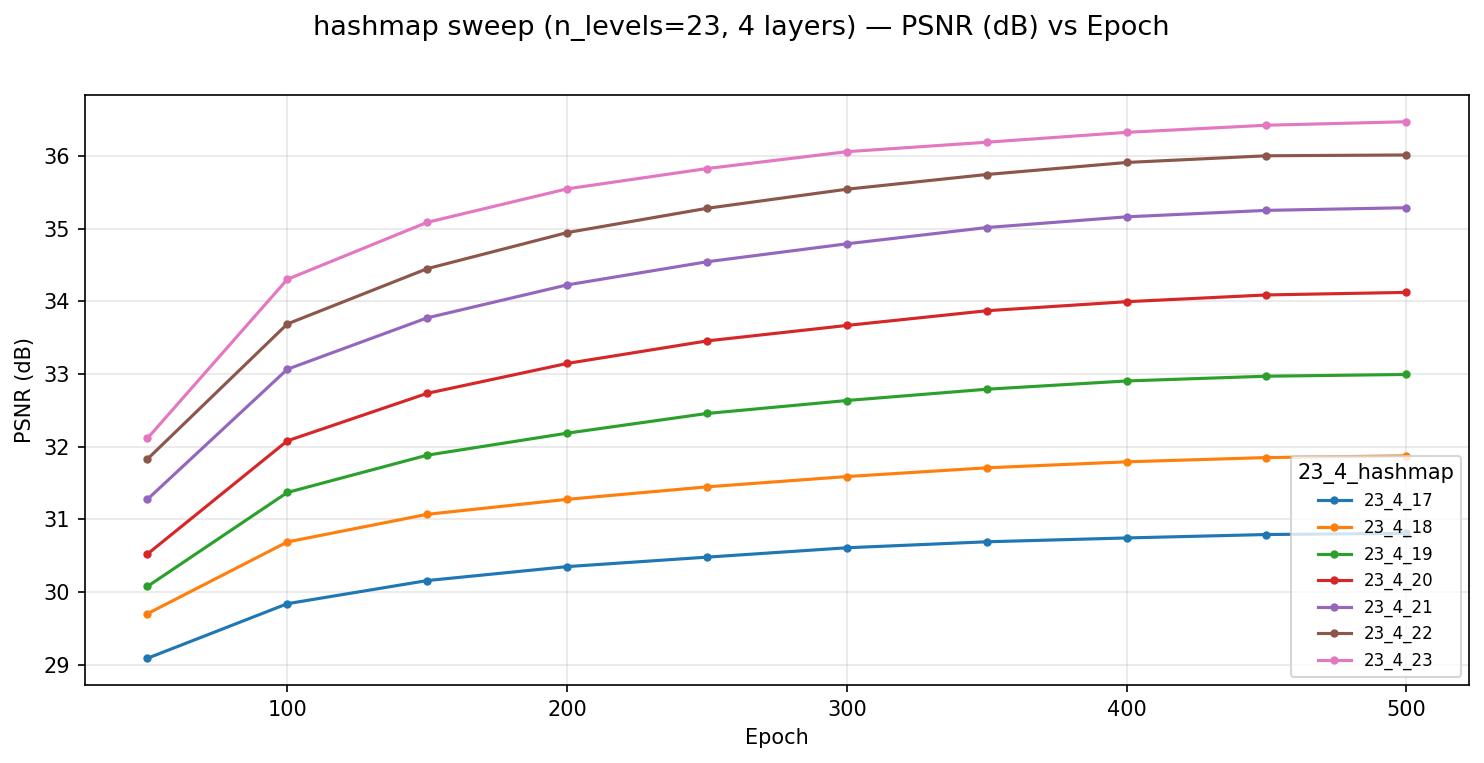
\includegraphics[width=1.1\textwidth]{hashmap23_plots/hashmap23_epoch_psnr.png}
    \end{adjustwidth}
    \caption{PSNR vs.\ epoch for $\log_2 T \in \{17,\ldots,23\}$ with $L = 23$ and $F = 4$ fixed.}
    \label{fig:epoch_hashmap}
\end{figure}

\begin{figure}[htbp]
    \begin{adjustwidth}{-2.5cm}{-2.5cm}
    \centering
    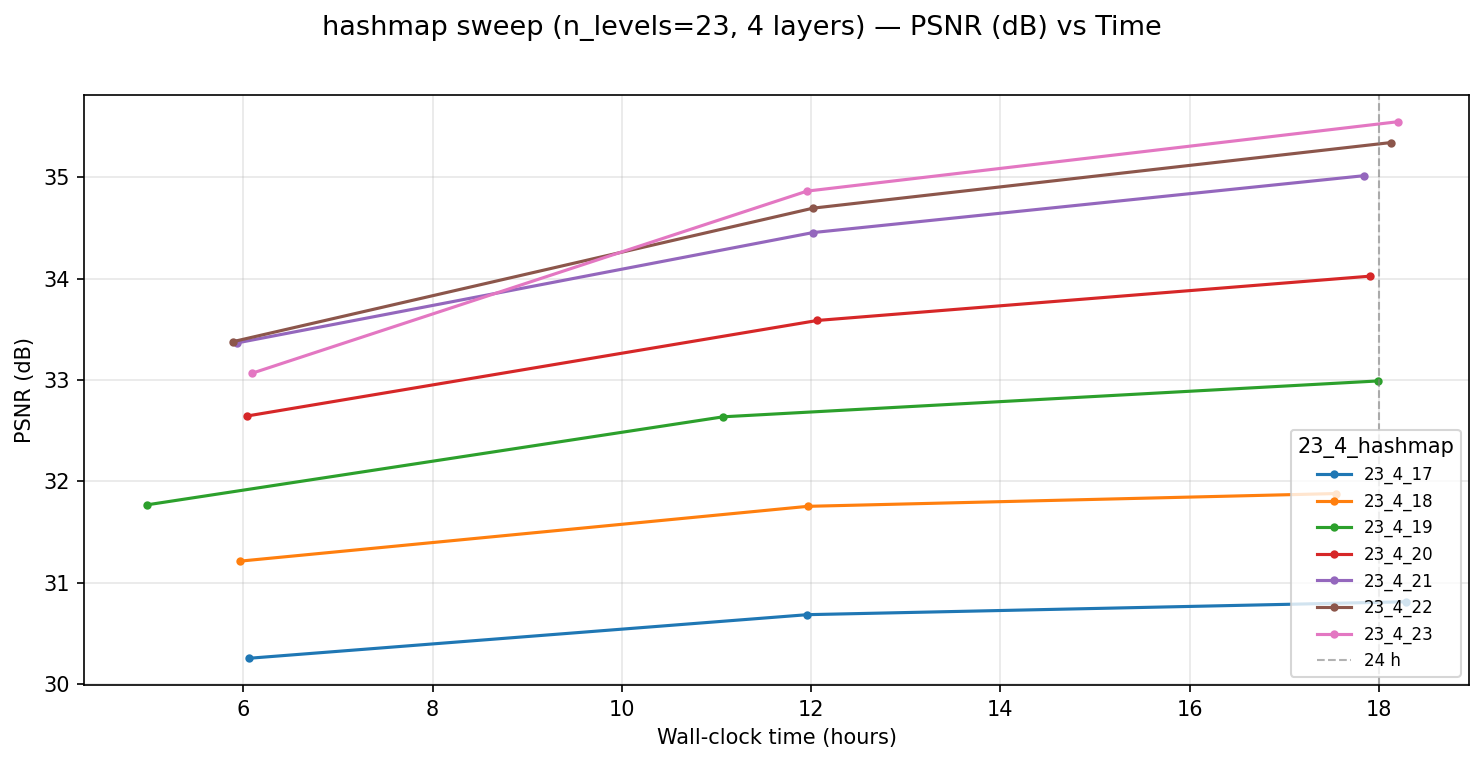
\includegraphics[width=1.1\textwidth]{hashmap23_plots/hashmap23_time_psnr.png}
    \end{adjustwidth}
    \caption{PSNR vs.\ wall-clock time for $\log_2 T \in \{17,\ldots,23\}$ with $L = 23$ and $F = 4$ fixed. Each curve is one hashmap size; the dashed vertical line marks the 18-hour budget.}
    \label{fig:time_hashmap}
\end{figure}

\begin{figure}[htbp]
    \begin{adjustwidth}{-2.5cm}{-2.5cm}
    \centering
    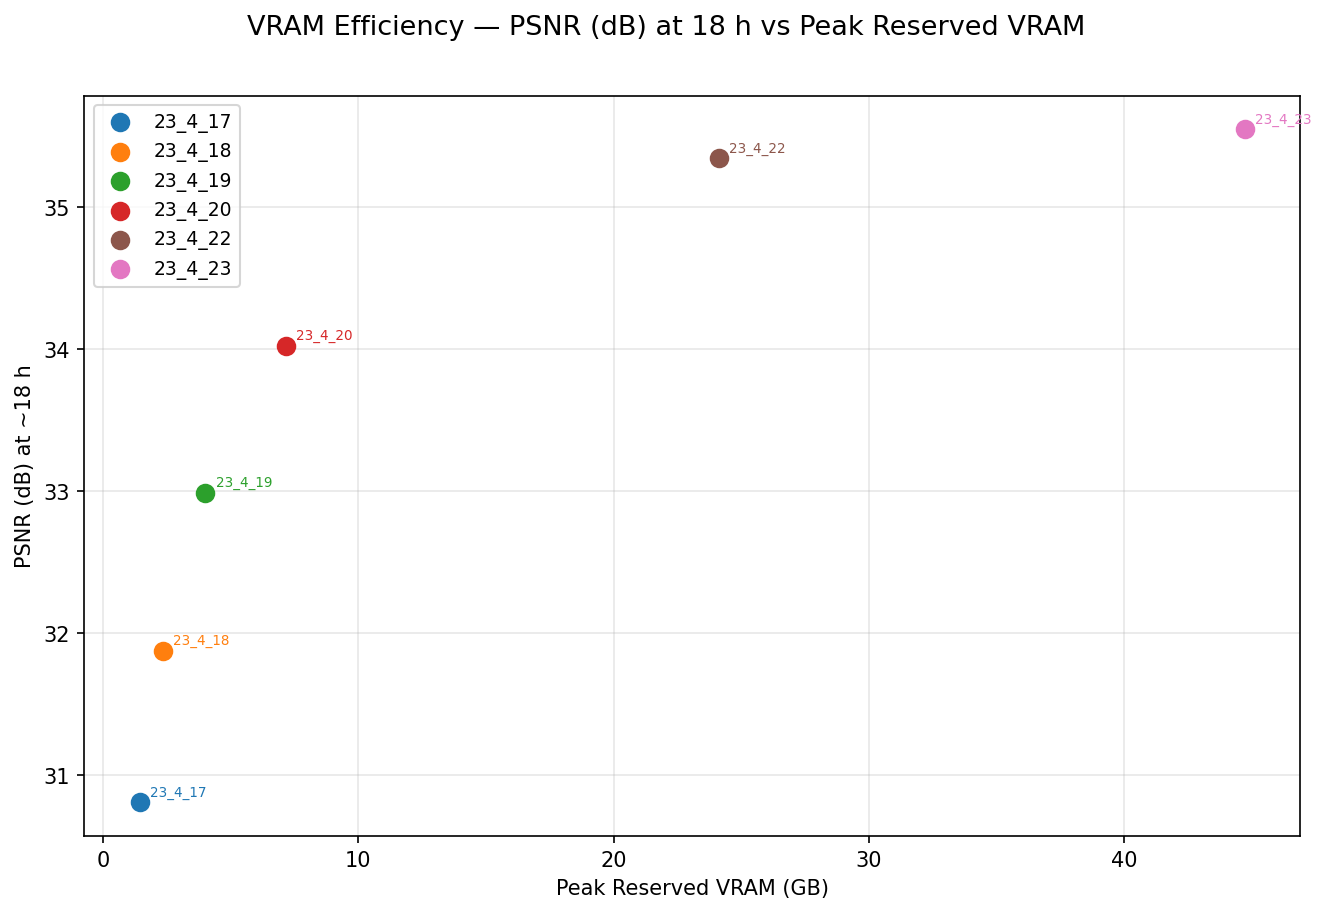
\includegraphics[width=1.1\textwidth]{hashmap23_plots/hashmap23_vram_psnr.png}
    \end{adjustwidth}
    \caption{PSNR at the 18-hour mark versus peak reserved VRAM for each $\log_2 T$ configuration ($L = 23$, $F = 4$). The near-linear relationship confirms that hashmap size is the dominant memory driver and that quality scales directly with allocated memory.}
    \label{fig:vram_hashmap}
\end{figure}

Figures~\ref{fig:epoch_hashmap}, \ref{fig:time_hashmap}, and \ref{fig:vram_hashmap} show a consistent pattern. Every reduction in hashmap size produces a corresponding drop in reconstruction quality across both the epoch and time axes. Each step down in $\log_2 T$ roughly halves the total encoder memory and doubles the finest-level collision rate. The configurations at $\log_2 T = 23$ and $\log_2 T = 22$ perform very similarly, suggesting quality is approaching saturation near the top of the range. At $\log_2 T = 21$ the model still converges to around 35\,dB PSNR, a meaningful result for many applications. Below $\log_2 T = 21$, however, all configurations plateau substantially lower and do not converge further, consistent with the collision rate having crossed the threshold where multi-level disambiguation can no longer recover sufficient spatial precision. The memory-versus-quality figure confirms that PSNR at 18 hours scales nearly linearly with peak VRAM. Smaller hashmaps should therefore only be chosen when GPU memory is the hard constraint, and $\log_2 T = 21$ represents a reasonable lower bound for acceptable reconstruction quality.

\subsection{SingleCube}
\label{subsec:singlecube}

The hashmap sweep operates entirely within the 3D QuadCubes encoder regime, where the baseline collision rate at $\log_2 T = 23$ is approximately 128 vertices per entry at the finest level, which is moderate and manageable. SingleCube extends the same encoder dimension to 4D with the same hashmap size, immediately increasing the finest-level collision rate to $N_\mathrm{max}^4 / T = 2^{17} \approx 131\,000$ vertices per entry. This is more than a thousand times the collision load of the baseline 3D encoders, and it occurs at every level that operates in the hashed regime.

The SingleCube architecture consists of a single 4D multiresolution hash encoder taking $(x, y, z, t)$ as input, which is conceptually the natural extension of the static NAF model from three to four dimensions. Rather than splitting the 4D space into overlapping 3D subproblems as QuadCubes does, it asks the encoder to represent the full space-time field directly. Figure~\ref{fig:singlecube_architecture} shows the architecture.

\begin{figure}[htbp]
    \centering
    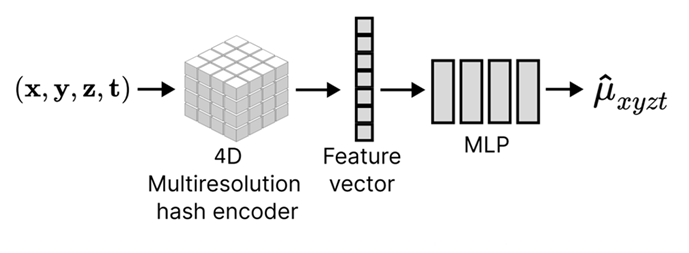
\includegraphics[width=0.70\textwidth]{arc_diagram/singlecube_diagram.png}
    \caption{The SingleCube architecture. A single 4D multiresolution hash encoder takes the full space-time coordinate $(x, y, z, t)$ as input and passes the concatenated multi-level features to a shared MLP decoder. The extreme collision load at $d=4$ makes this architecture infeasible at standard hashmap sizes.}
    \label{fig:singlecube_architecture}
\end{figure}

\begin{figure}[htbp]
    \begin{adjustwidth}{-2cm}{-2cm}
    \centering
    \begin{subfigure}[b]{0.6\textwidth}
        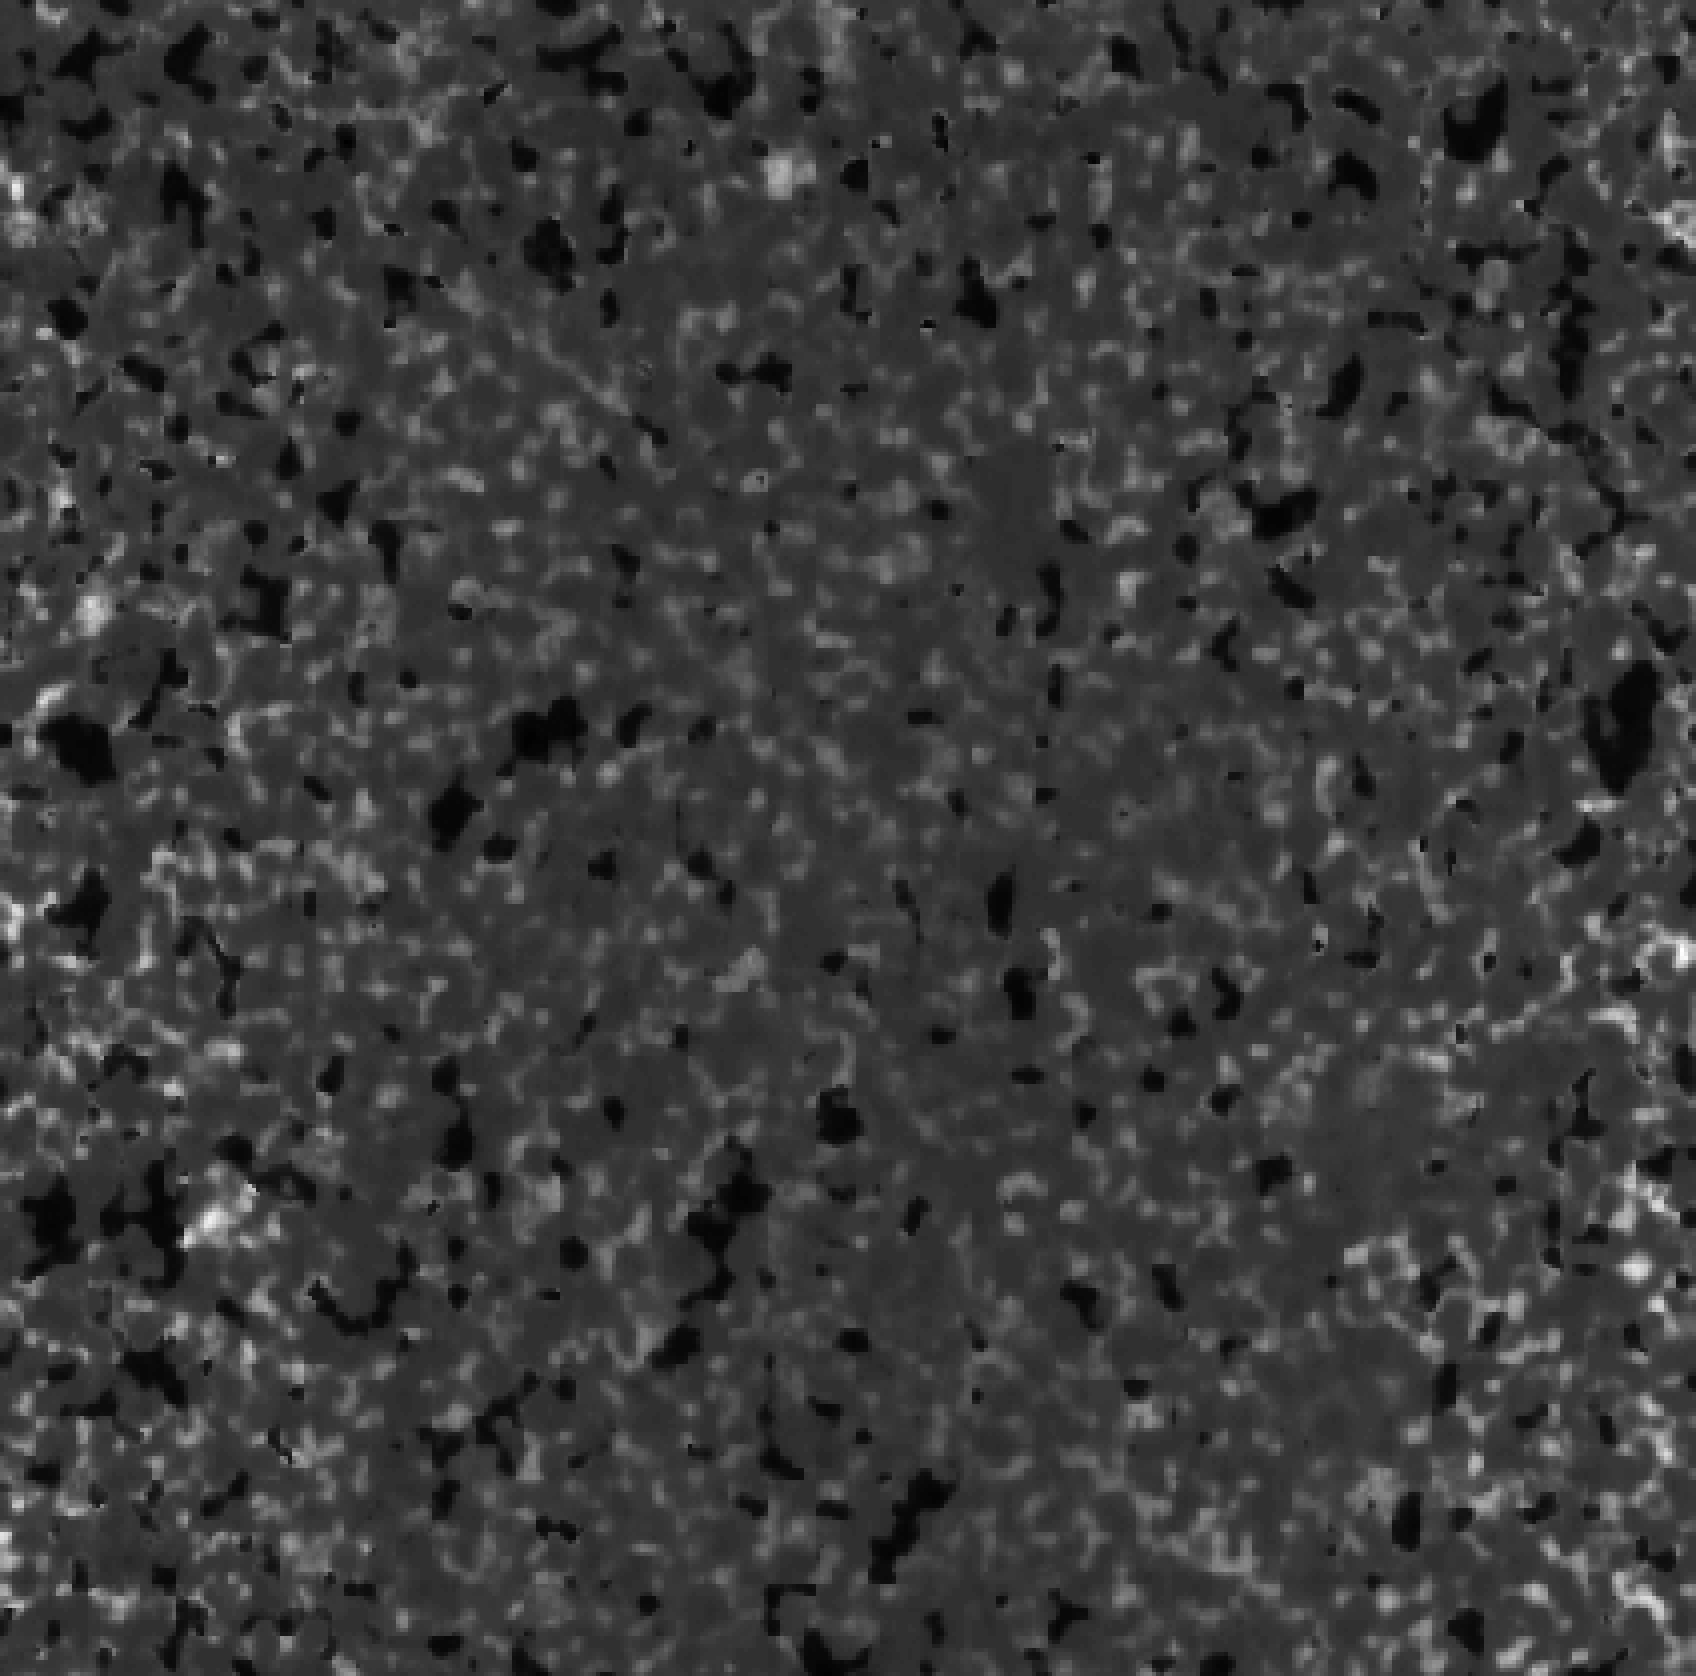
\includegraphics[width=\textwidth]{compairson.png}
        \caption{QuadCubes (reference)}
    \end{subfigure}
    \hfill
    \begin{subfigure}[b]{0.6\textwidth}
        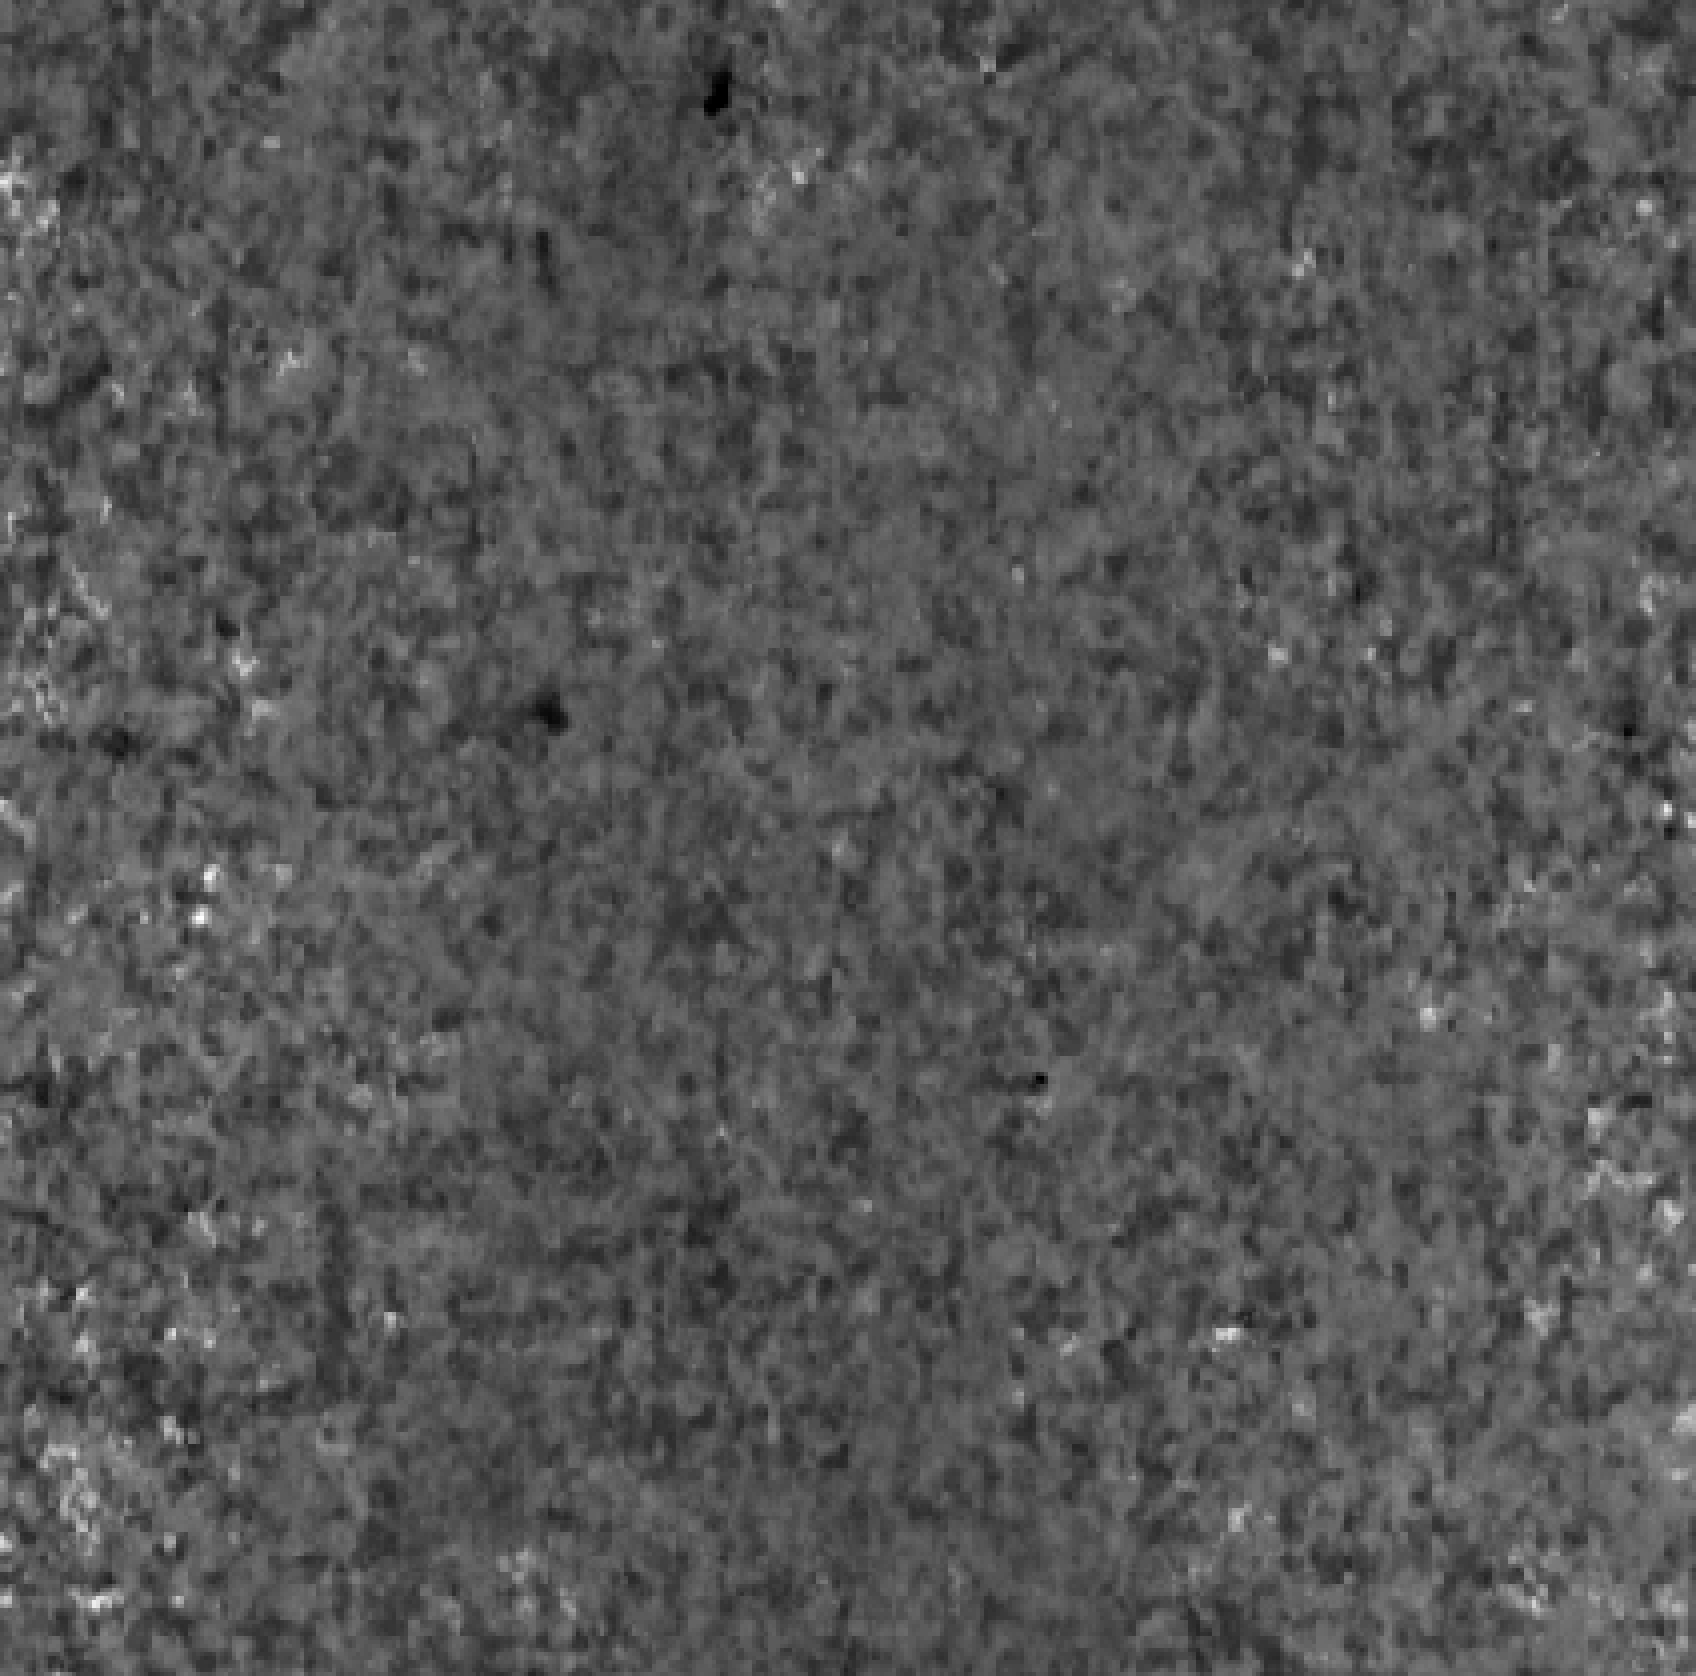
\includegraphics[width=\textwidth]{singlecube.png}
        \caption{SingleCube}
    \end{subfigure}
    \end{adjustwidth}
    \caption{Reconstruction comparison between QuadCubes and SingleCube at matched encoder capacity. The SingleCube output is dominated by noise from the extreme hash collision load in the 4D encoder.}
    \label{fig:singlecube_reconstruction}
\end{figure}

Figure~\ref{fig:singlecube_reconstruction} shows the result. The SingleCube output is dominated by pervasive noise. Even large clusters of high-attenuation material are only vaguely placed in approximately the correct location, with no discernible internal structure. The model cannot learn sharp features or their precise spatial placement because each stored feature vector is required to represent the average of more than 130\,000 distinct space-time locations. The MLP disambiguation mechanism, which uses context from other levels, is also compromised, since every level operates under the same severe collision regime with different hash functions but the same overload ratio.

The contrast with QuadCubes is direct. By decomposing the 4D problem into four 3D subproblems, QuadCubes reduces the finest-level collision rate from $2^{17}$ to $2^7 = 128$, a reduction of over three orders of magnitude, which is sufficient for the multi-level disambiguation to function as intended. The SingleCube experiment demonstrates that the architecture choice and the capacity choice are not independent. A larger hashmap at $d = 4$ would reduce the collision rate below $2^{17}$, but the memory required for a collision-free 4D encoder (64\,TB) makes this approach entirely infeasible.

\subsection{Precision and Collision Load}
\label{subsec:collision_synthesis}

The hashmap sweep establishes that within the 3D QuadCubes encoders, reducing hashmap size systematically degrades quality by increasing collision load, with a clear qualitative transition around $\log_2 T = 21$. Above this point models reach competitive PSNR, while below it they fail to converge to adequate precision regardless of training time. SingleCube shows that moving to 4D encoders with the same hashmap size makes the collision problem catastrophically worse. Together these findings establish the first design principle. The hashmap size should be chosen so that the collision rate at the finest resolution level is within the range where multi-level disambiguation is effective, and the encoder dimensionality should be chosen to keep that hashmap size within hardware limits.

For a 3D encoder at micro-CT resolutions, $\log_2 T = 23$ is at or near the quality saturation point. For a 4D encoder, no feasible hashmap size comes close. The QuadCubes decomposition is therefore not an arbitrary design choice but a practical necessity imposed by the collision constraint.

% ─────────────────────────────────────────────────────────────────────────────
\section{Levels, Coverage, and Coupling}
\label{sec:levels_and_coupling}
% ─────────────────────────────────────────────────────────────────────────────

Having established that hashmap size is the primary driver of model size and quality, this section examines the number of levels, which the theory predicts should primarily affect training time rather than model size, through its control of per-step computation cost and frequency coverage. The HexCubes architecture then illustrates what happens when frequency coverage is ample and collision rates are low, but the encoder can represent only pairwise coordinate interactions, a situation that places an unusually heavy burden on the decoder.

\subsection{Number of Levels Sweep in QuadCubes}
\label{subsec:levels_sweep}

Values of $L \in \{17, 18, 19, 20, 21, 22, 23\}$ were evaluated with $\log_2 T = 23$ and $F = 4$ held fixed. Reducing $L$ from 23 to 17 removes six levels from the top of the frequency hierarchy, eliminating the finest-scale features while keeping the coarse structure intact. At the same time, each removed level reduces the number of hash table lookups and MLP input features per training step, directly reducing the per-step computation and therefore the wall-clock time per epoch.

\begin{figure}[htbp]
    \begin{adjustwidth}{-2.5cm}{-2.5cm}
    \centering
    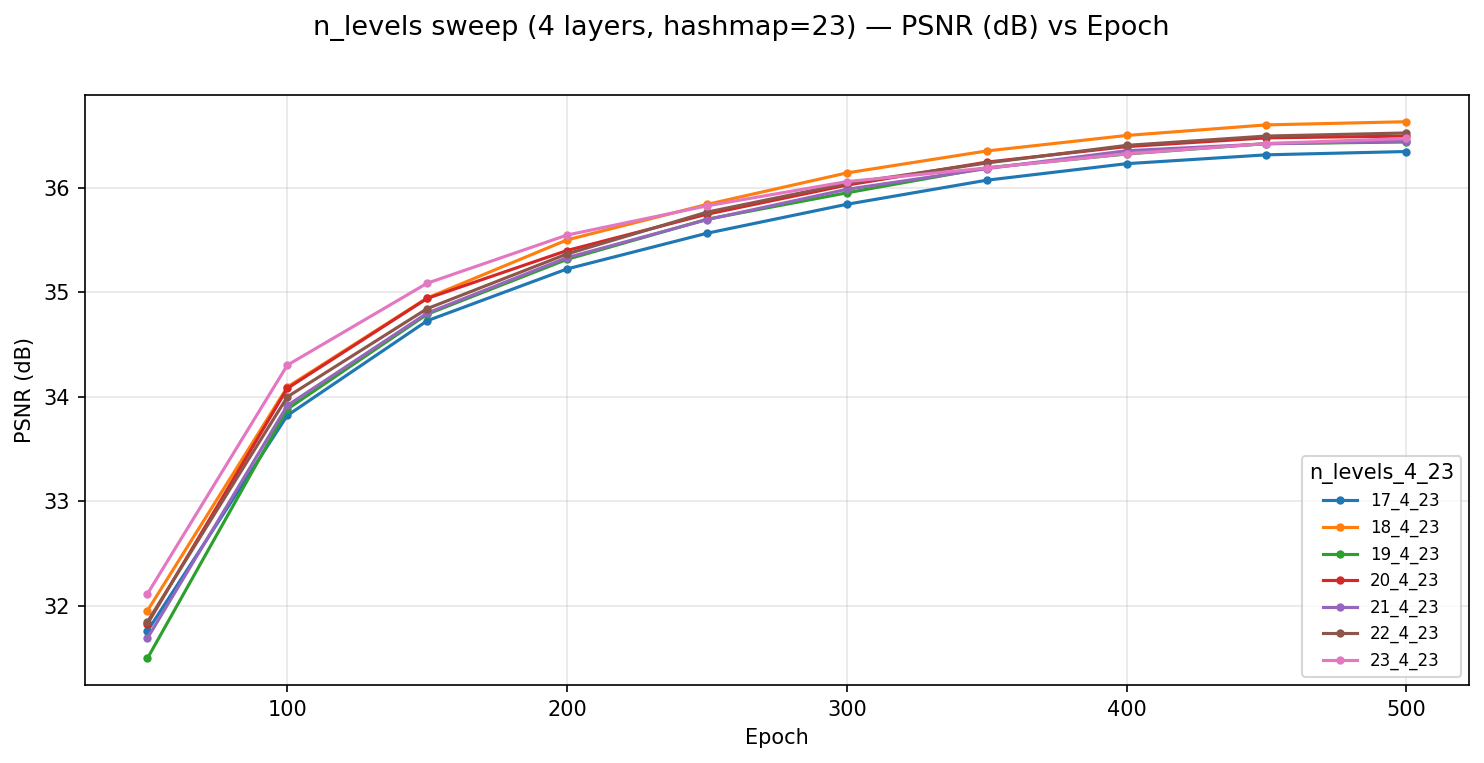
\includegraphics[width=1.1\textwidth]{nlevel_plots/nlevel_epoch_psnr.png}
    \end{adjustwidth}
    \caption{PSNR vs.\ epoch for $L \in \{17,\ldots,23\}$ with $\log_2 T = 23$ and $F = 4$ fixed.}
    \label{fig:levels_epoch}
\end{figure}

\begin{figure}[htbp]
    \begin{adjustwidth}{-2.5cm}{-2.5cm}
    \centering
    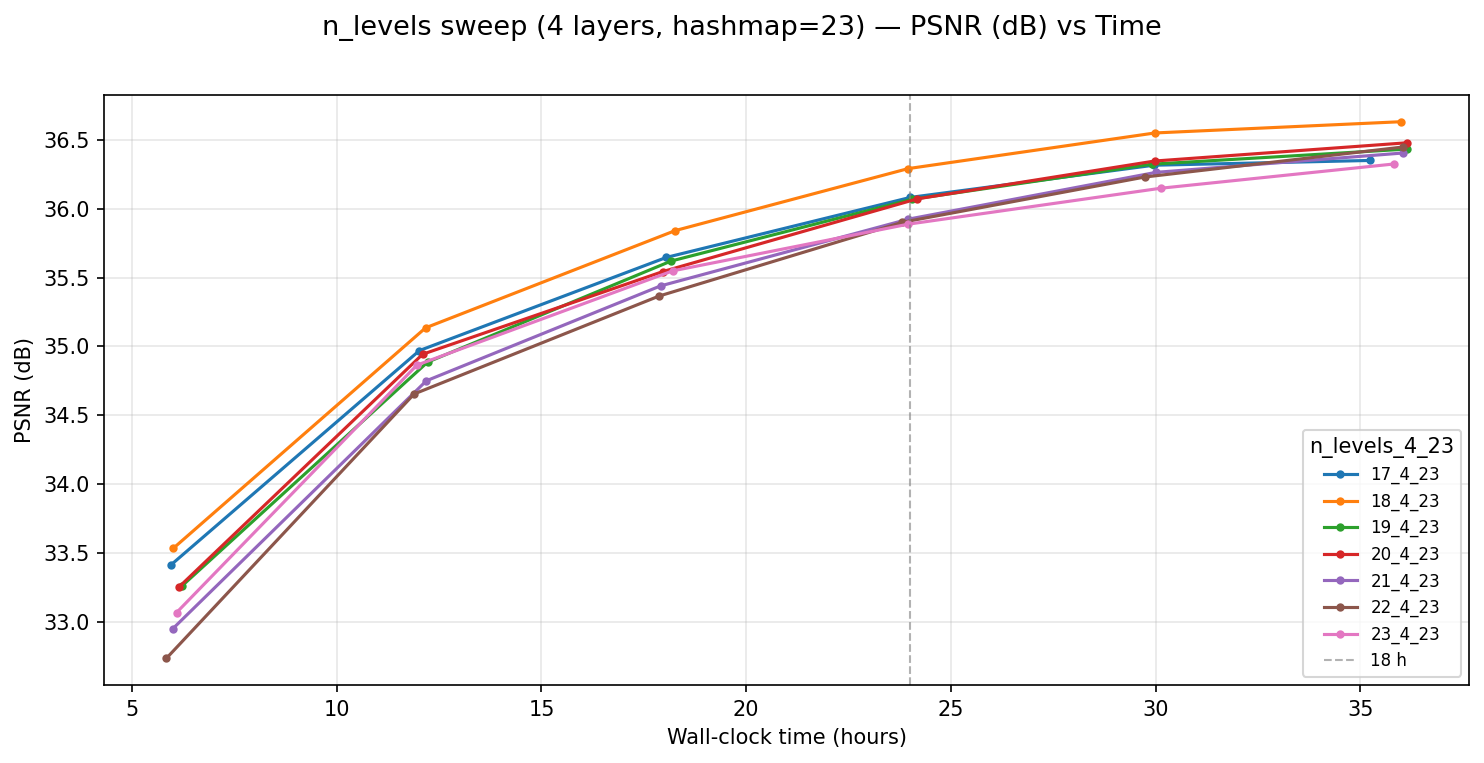
\includegraphics[width=1.1\textwidth]{nlevel_plots/nlevel_time_psnr.png}
    \end{adjustwidth}
    \caption{PSNR vs.\ wall-clock time for $L \in \{17,\ldots,23\}$ with $\log_2 T = 23$ and $F = 4$ fixed. Each curve is one level count; the dashed vertical line marks the 24-hour budget.}
    \label{fig:levels_time}
\end{figure}

\begin{figure}[htbp]
    \begin{adjustwidth}{-2.5cm}{-2.5cm}
    \centering
    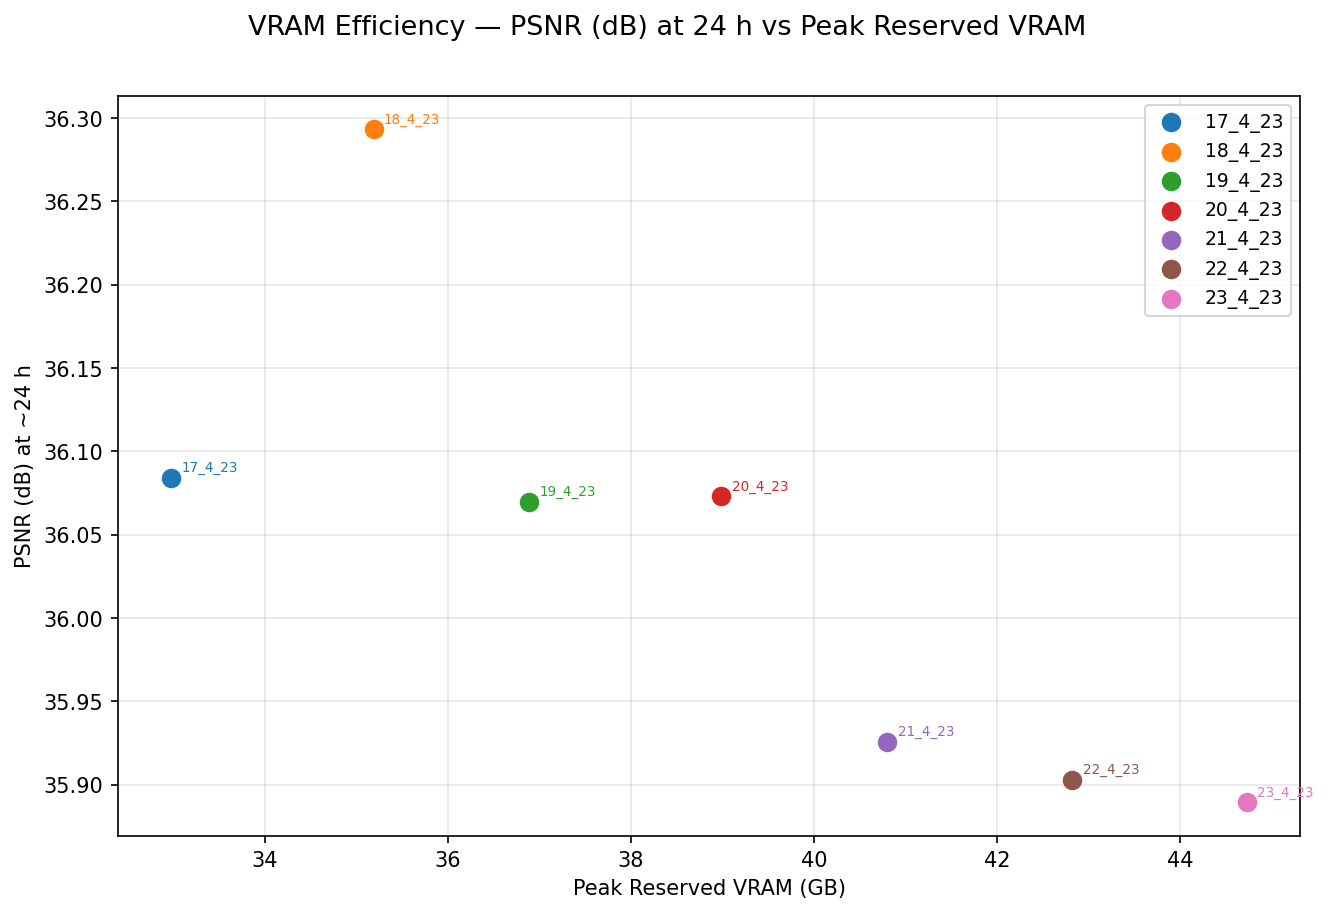
\includegraphics[width=1.1\textwidth]{nlevel_plots/nlevel_vram_psnr.png}
    \end{adjustwidth}
    \caption{PSNR at the 24-hour mark versus peak reserved VRAM for each $L$ configuration ($\log_2 T = 23$, $F = 4$). Unlike the hashmap sweep, quality is largely decoupled from memory usage, confirming that the level count is not a meaningful memory driver.}
    \label{fig:vram_levels}
\end{figure}

The results contrast with the hashmap sweep. In the epoch plot the curves are tightly clustered, with all values of $L$ converging to nearly the same asymptotic PSNR, indicating that the dataset complexity is well within the representational capacity of even the smallest level count tested. Removing the finest levels does not meaningfully limit the model's ultimate precision. What does differ is the speed of convergence. Configurations with fewer levels reach their asymptote in fewer epochs, since each step is cheaper to compute. The asymptotic quality is essentially the same whether the model uses 17 or 23 levels, meaning the additional levels in the baseline contribute training-time cost without returning quality.

The wall-clock time plot makes the practical implication clear. $L = 18$ stands out as the best-performing configuration across both axes, converging faster than larger level counts and achieving the highest PSNR within the 24-hour budget, combining the speed advantage of a shallow hierarchy with sufficient frequency coverage for this dataset. Configurations with $L < 18$ converge quickly but plateau slightly lower, suggesting that 18 levels captures the last meaningful frequency band for this data. Configurations with $L > 18$ offer no quality gain and train more slowly. The VRAM plot reinforces this from a memory perspective. PSNR at 24 hours is nearly flat across all level counts despite the varying VRAM footprint, in contrast to the hashmap sweep. The level count therefore acts primarily as a training-time dial rather than a quality or memory dial, confirming the theoretical prediction. The practical recommendation for QuadCubes is to use $L = 18$ rather than the baseline $L = 23$, saving approximately one quarter of per-epoch training time with no quality penalty.

Across all architectures evaluated in this chapter, the spatial encoder is sensitive to level count in a different way from the temporal encoders. For the spatial 3D encoder, $L = 17$ and below is generally insufficient to capture the full frequency content of micro-CT pore geometry, and quality degrades noticeably. The temporal 2D encoders in CombinedCubes and \MixedCubes{} are less demanding. Their lower-frequency signal allows the level count to be reduced to $L = 15$ without meaningful quality loss, providing additional training-time savings in the split-encoder architectures.

\subsection{Features Per Level}
\label{subsec:features_sweep}

Values of $F \in \{1, 2, 4\}$ were evaluated with $L = 23$ and $\log_2 T = 23$ held fixed. Reducing $F$ halves both the encoder memory and the MLP input dimension per step (from $4 \times 23 \times 4 = 368$ to 184 features at $F = 2$, and to 92 at $F = 1$), so unlike the level count, $F$ affects both memory and computation proportionally.

\begin{figure}[htbp]
    \begin{adjustwidth}{-2.5cm}{-2.5cm}
    \centering
    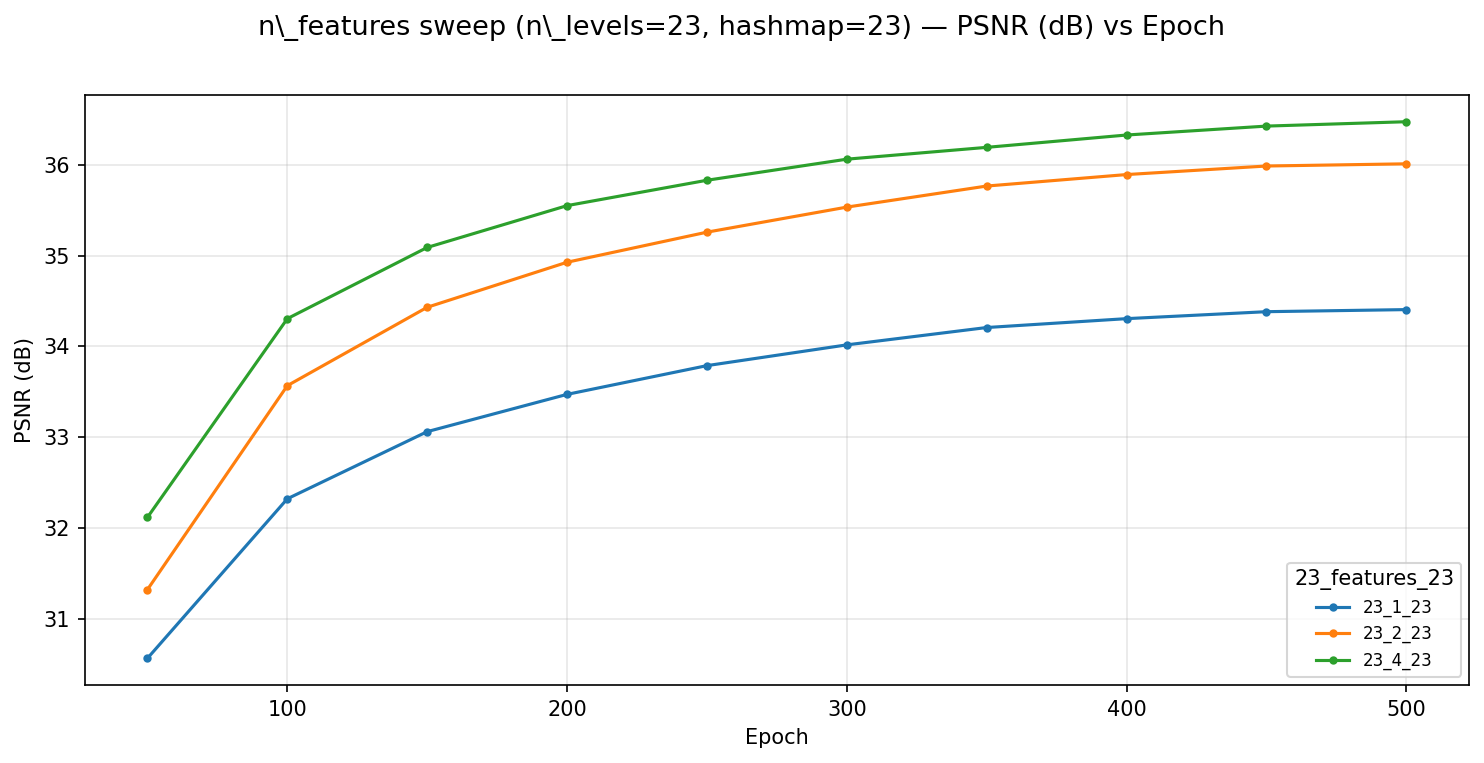
\includegraphics[width=1.1\textwidth]{features_plots/features_epoch_psnr.png}
    \end{adjustwidth}
    \caption{PSNR vs.\ epoch for $F \in \{1, 2, 4\}$ with $L = 23$ and $\log_2 T = 23$ fixed.}
    \label{fig:features_epoch}
\end{figure}

\begin{figure}[htbp]
    \begin{adjustwidth}{-2.5cm}{-2.5cm}
    \centering
    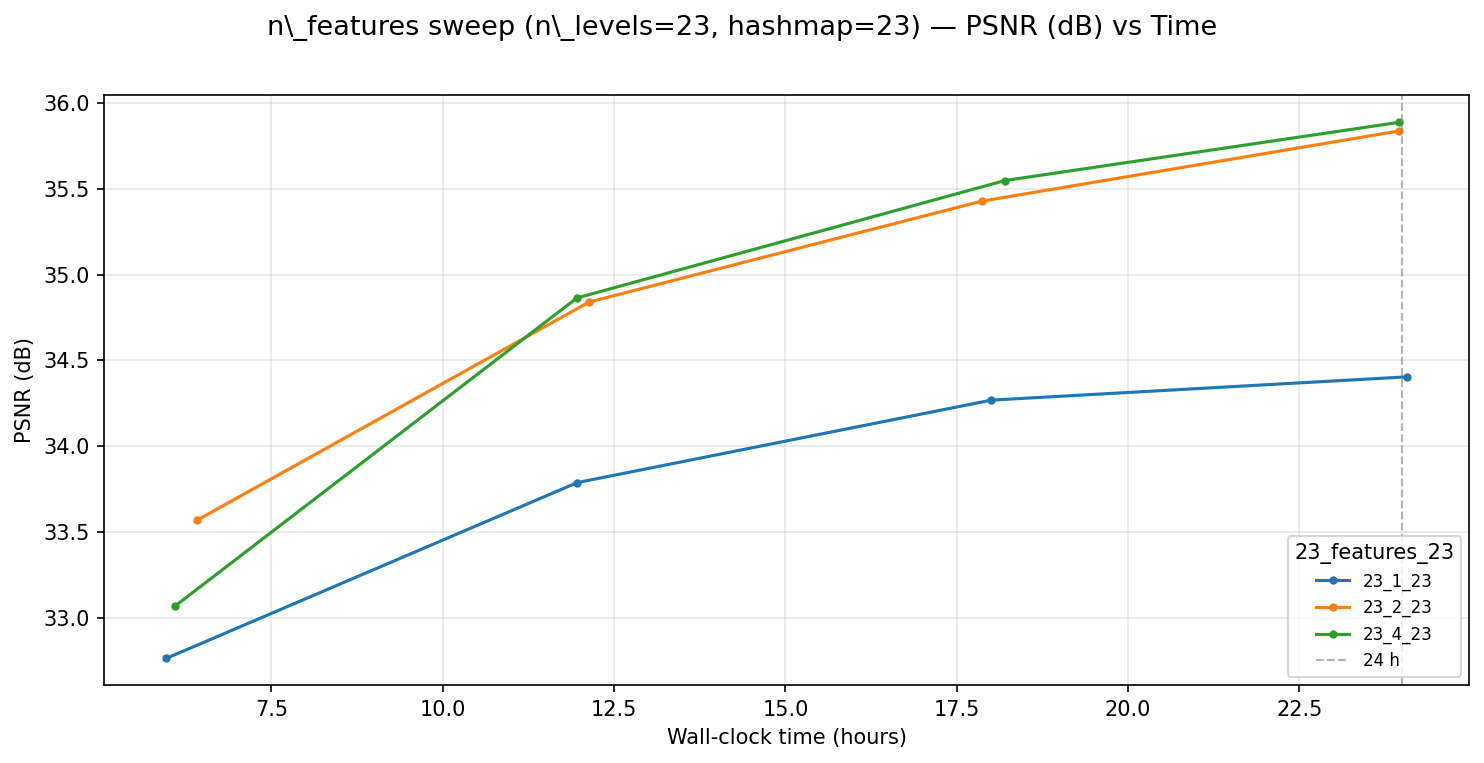
\includegraphics[width=1.1\textwidth]{features_plots/features_time_psnr.png}
    \end{adjustwidth}
    \caption{PSNR vs.\ wall-clock time for $F \in \{1, 2, 4\}$ with $L = 23$ and $\log_2 T = 23$ fixed. Each curve is one feature count; the dashed vertical line marks the 24-hour budget.}
    \label{fig:features_time}
\end{figure}

\begin{figure}[htbp]
    \begin{adjustwidth}{-2.5cm}{-2.5cm}
    \centering
    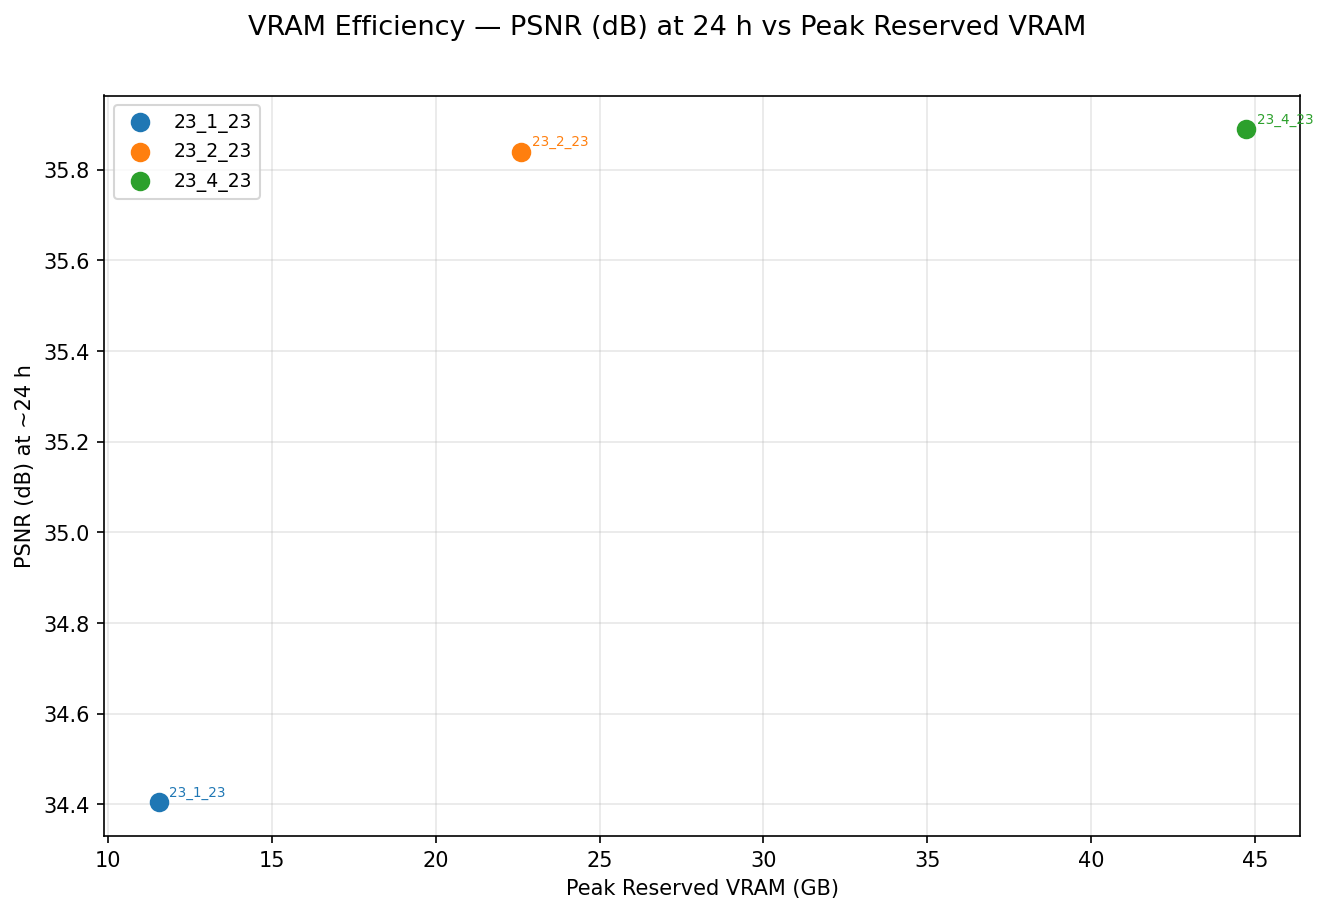
\includegraphics[width=1.1\textwidth]{features_plots/features_vram_psnr.png}
    \end{adjustwidth}
    \caption{PSNR at the 24-hour mark versus peak reserved VRAM for $F \in \{1, 2, 4\}$ ($L = 23$, $\log_2 T = 23$). Halving $F$ from 4 to 2 roughly halves VRAM with negligible quality loss.}
    \label{fig:vram_features}
\end{figure}

The results reveal a clear three-way split. $F = 1$ fails to converge. The encoder lacks sufficient capacity to represent the spatial features at any point during training, and PSNR remains stuck well below the other configurations. The failure is consistent across both axes and shows no sign of catching up with additional training, indicating a hard capacity floor rather than a convergence speed issue.

$F = 2$ is surprisingly competitive with $F = 4$ in the epoch plot, reaching a very similar asymptotic PSNR, indicating that halving the feature dimension does not meaningfully limit what the model can ultimately represent within the uniform QuadCubes architecture. In the wall-clock time plot the $F = 2$ and $F = 4$ curves are practically indistinguishable, because the reduced input dimension also speeds up each training step. The VRAM figure confirms that $F = 2$ achieves equivalent quality at roughly half the peak VRAM. This finding holds within the uniform QuadCubes architecture where all encoders are over-provisioned.

However, this result does not transfer to the split-encoder architectures evaluated in the later sections. In CombinedCubes and \MixedCubes{}, configurations with $F = 2$ on the temporal encoders consistently underperform relative to $F = 4$ equivalents at comparable VRAM, and in some cases fall below the QuadCubes baseline entirely. The difference is structural. In the uniform QuadCubes setting, $F = 2$ removes redundant capacity from already over-provisioned encoders. In the split-encoder setting, the temporal encoders are small and targeted, and halving $F$ removes capacity that the encoder genuinely needs. The practical implication is that $F = 2$ is beneficial as a reduction within the QuadCubes family, but $F = 4$ should be retained when switching to the split-encoder architectures.

\subsection{HexCubes}
\label{subsec:sexcubes}

\begin{figure}[htbp]
    \centering
    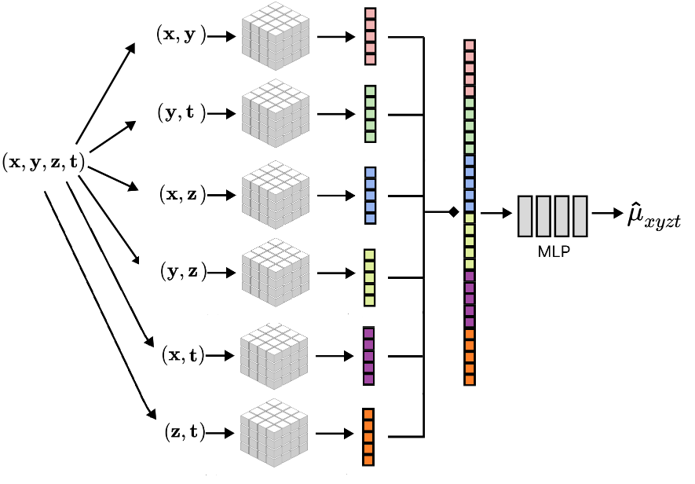
\includegraphics[width=0.80\textwidth]{arc_diagram/hexcubes_diagram.png}
    \caption{The HexCubes architecture. Six 2D multiresolution hash encoders cover all six coordinate pairs from the four space-time dimensions ($xy$, $xz$, $yz$, $xt$, $yt$, $zt$). Features from all six encoders are concatenated and decoded by a shared MLP. Each individual encoder is collision-free at practical 2D resolutions, but the MLP must infer three- and four-way coordinate interactions from pairwise features alone.}
    \label{fig:hexcubes_architecture}
\end{figure}

\begin{figure}[htbp]
    \begin{adjustwidth}{-2cm}{-2cm}
    \centering
    \begin{subfigure}[b]{0.5\textwidth}
        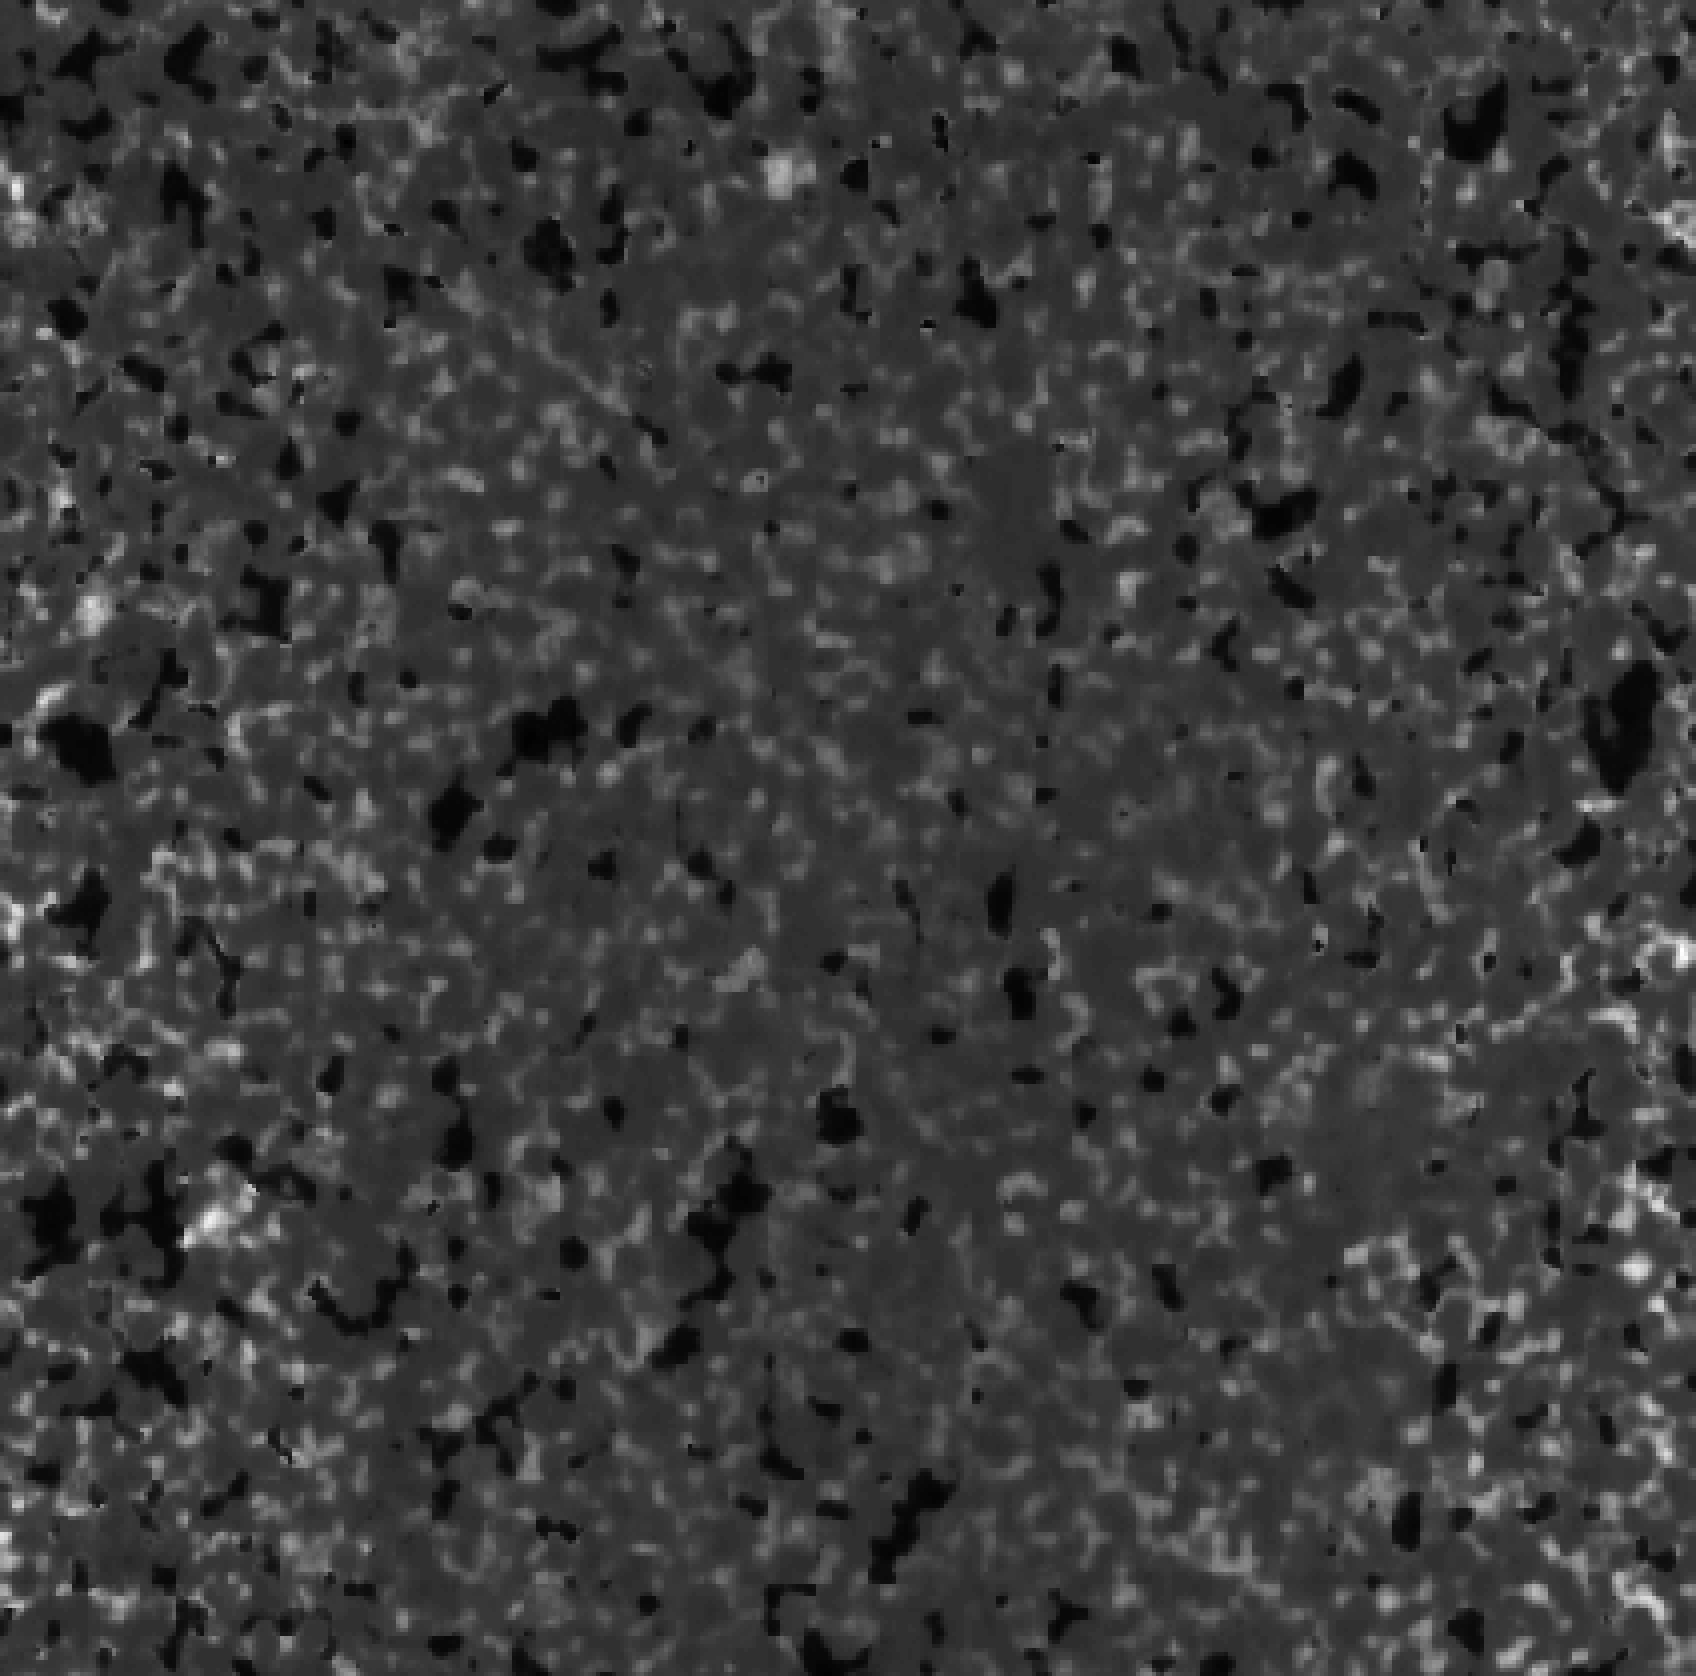
\includegraphics[width=\textwidth]{compairson.png}
        \caption{QuadCubes (ref.)}
    \end{subfigure}
    \hspace{0.1cm}
    \begin{subfigure}[b]{0.5\textwidth}
        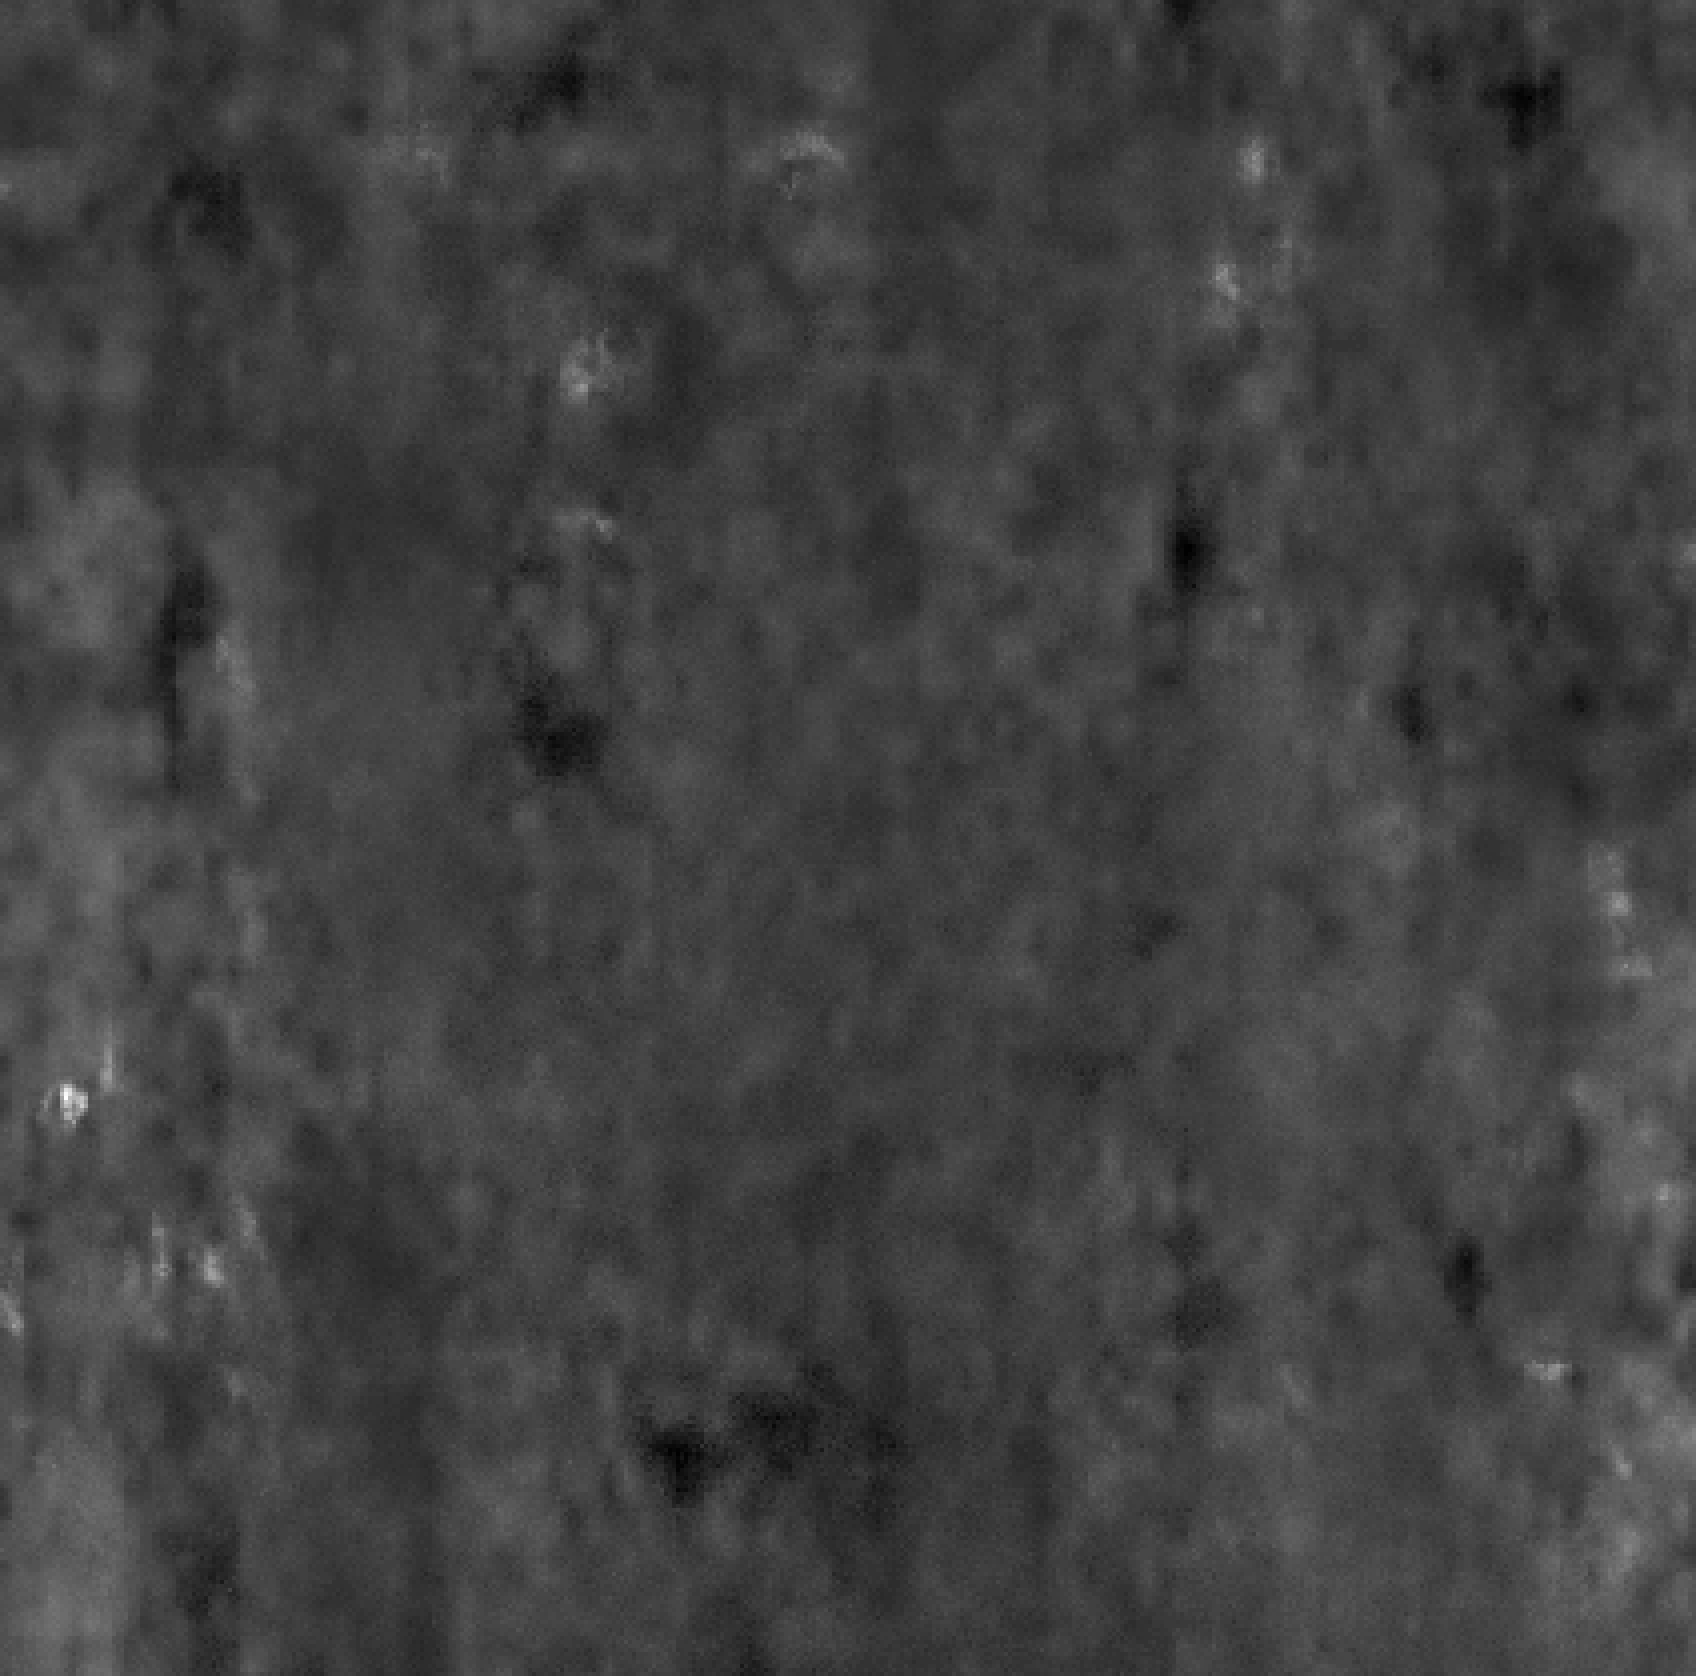
\includegraphics[width=\textwidth]{sexcubes_128_4.png}
        \caption{HexCubes, 4 hidden layers}
    \end{subfigure}
    \hspace{0.1cm}
    \begin{subfigure}[b]{0.5\textwidth}
        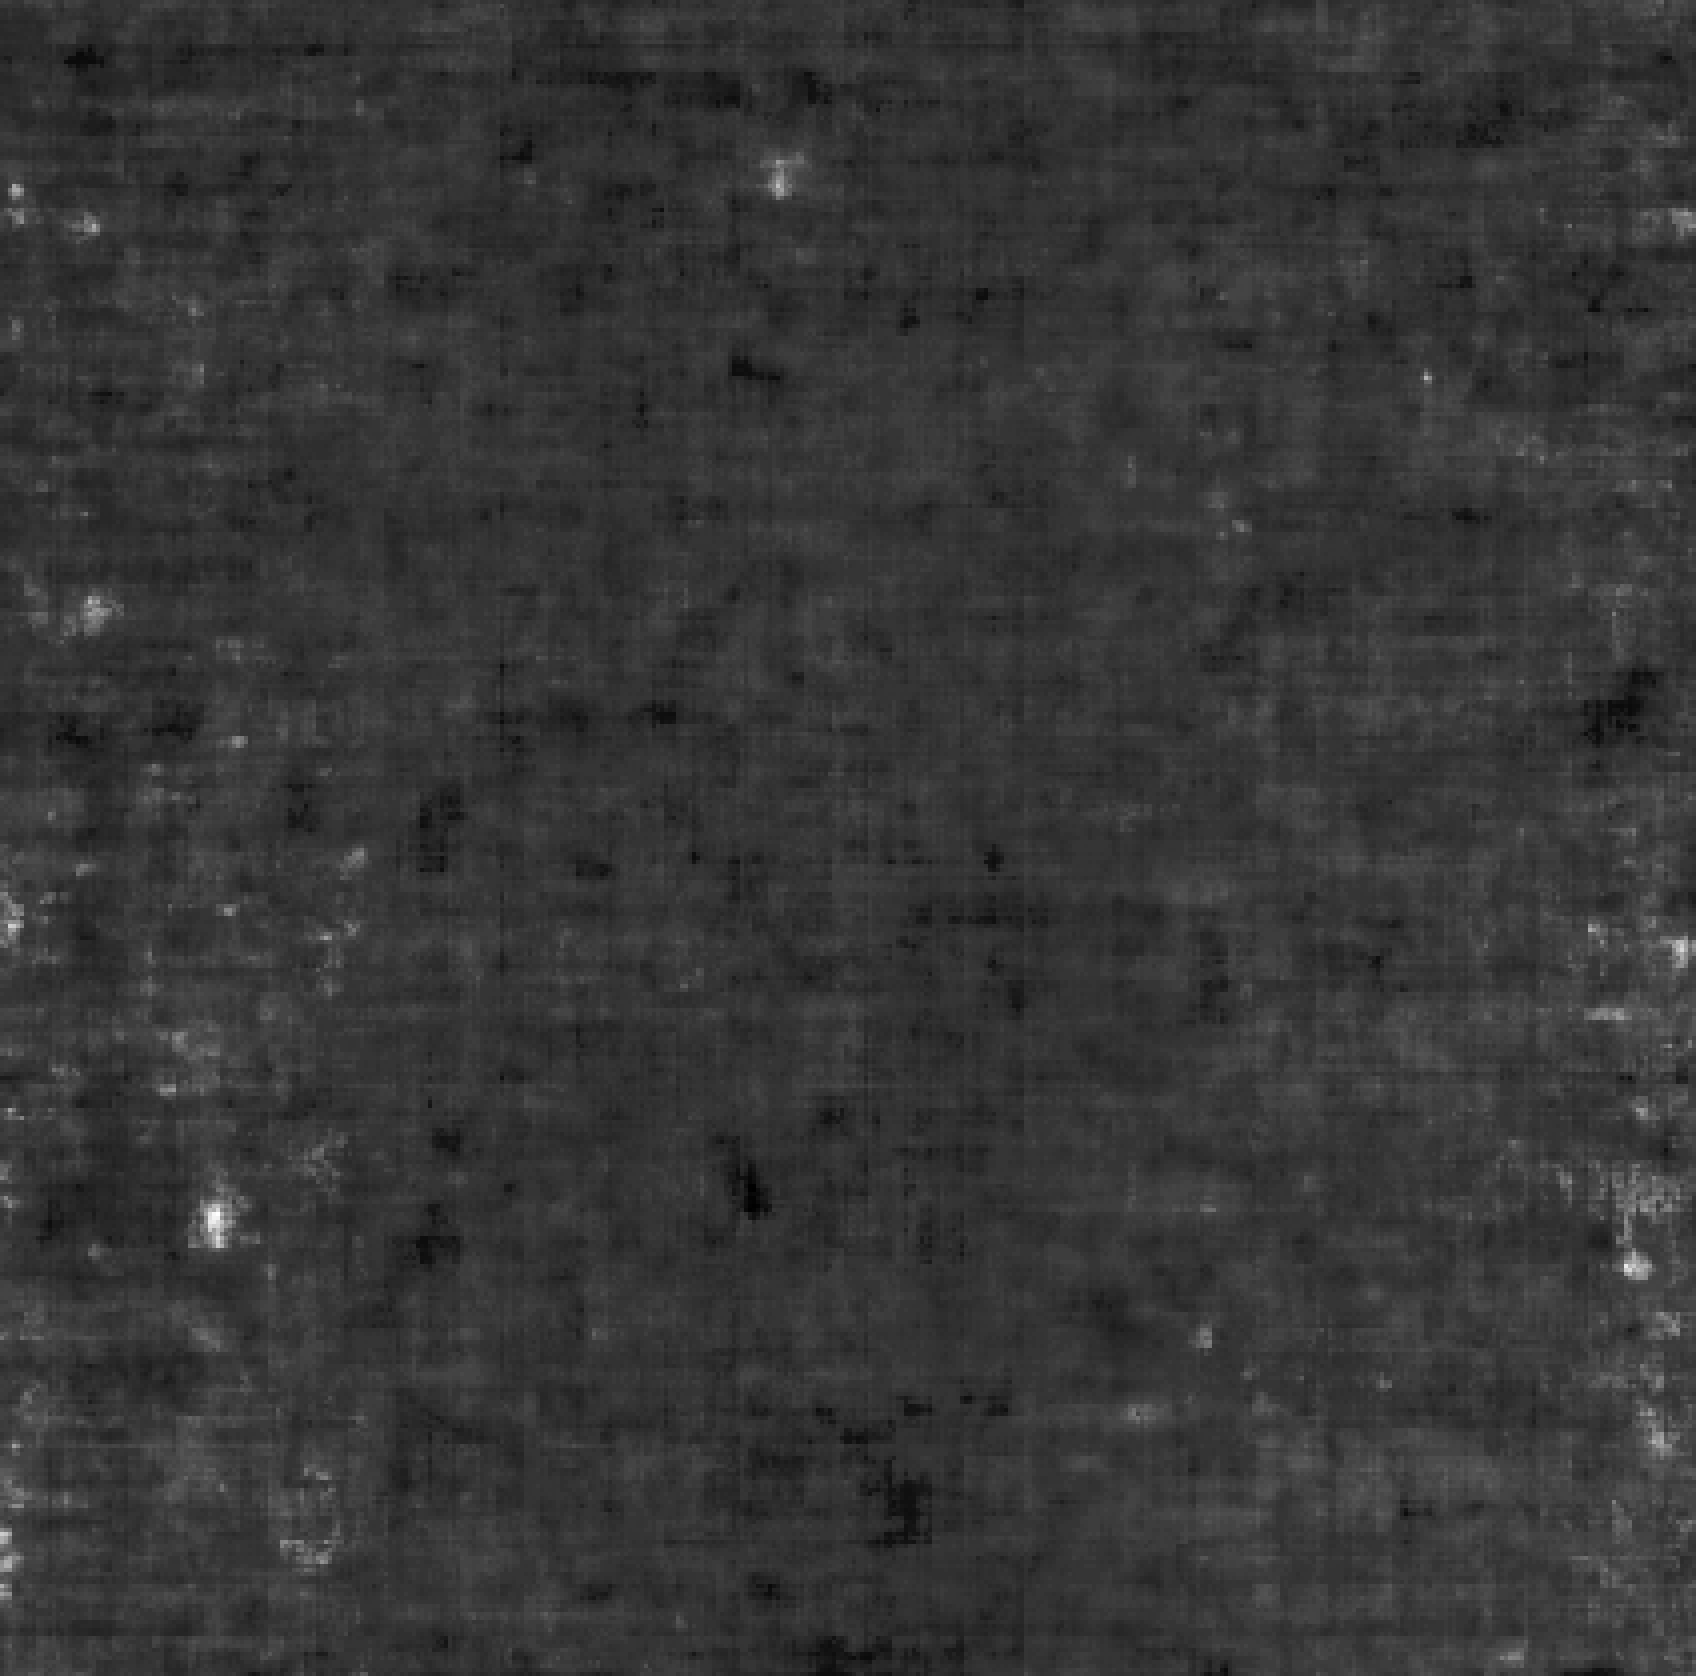
\includegraphics[width=\textwidth]{sexcubes_128_7.png}
        \caption{HexCubes, 7 hidden layers}
    \end{subfigure}
    \hspace{0.1cm}
    \begin{subfigure}[b]{0.5\textwidth}
        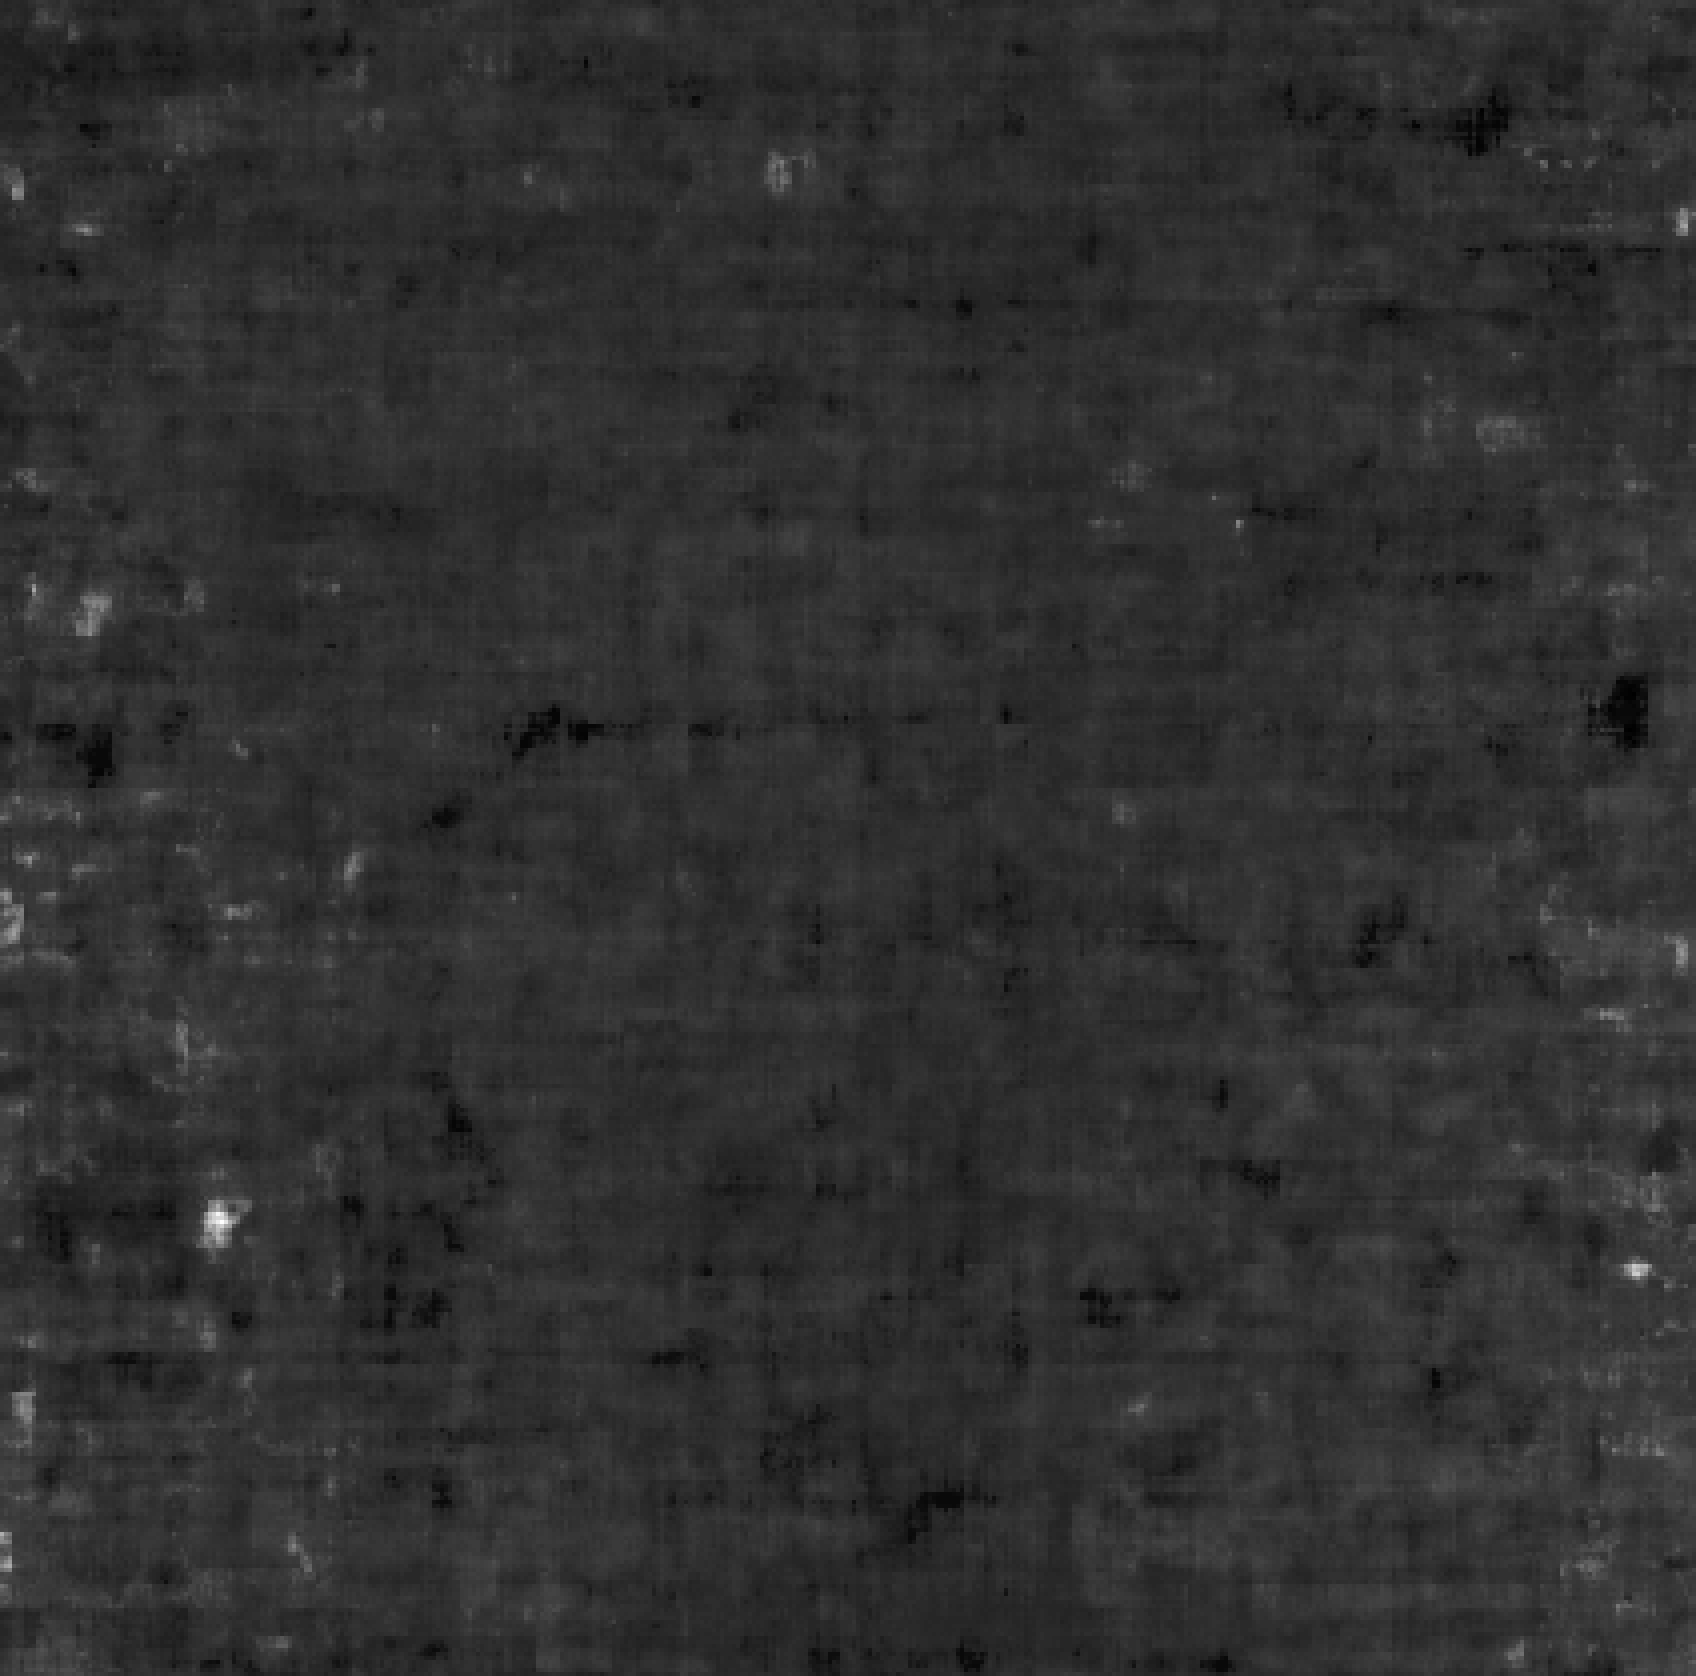
\includegraphics[width=\textwidth]{sexcubes_128_16.png}
        \caption{HexCubes, 16 hidden layers}
    \end{subfigure}
    \end{adjustwidth}
    \caption{Reconstruction comparison between QuadCubes and HexCubes with 128 neurons per hidden layer and varying decoder depth. Structural patterns emerge from 7 layers onwards but the architecture does not converge to the QuadCubes quality level even at 16 layers.}
    \label{fig:sexcubes_reconstruction}
\end{figure}

The level sweep established that reducing $L$ saves training time at the cost of frequency coverage. HexCubes takes a different approach to the time problem. Rather than reducing the number of levels, it replaces the four 3D encoders of QuadCubes with six 2D encoders, one for each possible pair of the four coordinates $\{x, y, z, t\}$. This reduces collision load considerably. A 2D encoder with $\log_2 T = 20$ is collision-free at resolutions up to $1024 \times 1024$, and memory falls to approximately 768\,MB for six encoders, roughly one eighth the baseline. The architecture follows the approach of K-Planes \citep{fridovichkeil2023kplanes} and HexPlane \citep{cao2023hexplane} for dynamic novel-view synthesis.

The cost of this design is that each encoder captures only pairwise coordinate interactions. Reconstructing the attenuation at $(x, y, z, t)$ from six 2D plane projections is analogous to recovering a 4D function from its six 2D marginals, which is formally underdetermined without additional coupling assumptions. The MLP must infer the missing higher-order interactions from the pairwise features alone, which is a harder integration task than in the 3D encoder case where each encoder already encodes three-way interactions.

\subsubsection{MLP Decoder Depth}

Figure~\ref{fig:sexcubes_reconstruction} shows the reconstruction quality as a function of decoder depth. At 4 hidden layers the output is unrecognisable. At 7 layers clear structural patterns appear and the reconstruction becomes recognisable. Increasing depth to 16 layers, however, produces a worse result than 7 layers rather than a better one. Without regularisation such as dropout, a deeper MLP in this setting overfits to noise in the pairwise feature inputs rather than learning to integrate them into coherent spatial structure. The 2D encoders provide only marginal information per coordinate pair, and a very deep decoder amplifies inconsistencies in those features rather than resolving them. This non-monotonic behaviour with depth shows that the fundamental limitation of HexCubes is not insufficient decoder capacity but insufficient encoder information. The missing three-way and four-way coordinate interactions cannot be recovered by any MLP, regardless of depth, because they were never encoded in the first place.

\subsection{Precision and Training Time}
\label{subsec:levels_synthesis}

The level sweep established that reducing $L$ is the primary lever for improving quality per unit of training time, since each removed level reduces per-step computation without proportionally reducing model size or quality ceiling. The equalised-time comparison confirms this. Configurations with fewer levels and smaller hashmaps can complete more training iterations within the same wall-clock budget and thereby achieve better reconstructions than the over-provisioned baseline.

HexCubes demonstrates the limit of this reasoning. Collision-free 2D encoders with low per-step cost achieve ample frequency coverage but fail to encode the higher-order coordinate interactions that the MLP needs to reconstruct 3D spatial structure. Increasing decoder depth can partially compensate, but the improvement saturates well below the QuadCubes reference, as a deeper MLP cannot recover coordinate interactions that the encoders never captured. The second design principle follows from this. The encoder dimensionality must be high enough to capture the coordinate interactions that the reconstruction problem requires, and the number of levels should be tuned to the training time budget rather than maximised.

% ─────────────────────────────────────────────────────────────────────────────
\section{Spatial-Temporal Asymmetry}
\label{sec:spatial_temporal_asym}
% ─────────────────────────────────────────────────────────────────────────────

The two preceding sections treated all four QuadCubes encoders uniformly, with the same hashmap size, the same number of levels, and the same features per level. The theory in \cref{subsec:spatial_temporal_theory} gave reason to expect that this is suboptimal, because the spatial encoder and the temporal encoders have different gradient update densities, different signal properties, and therefore different capacity requirements. This section tests that hypothesis quantitatively through non-uniform sizing experiments within QuadCubes, and then demonstrates its structural consequence in the CombinedCubes and \MixedCubes{} architectures.

\subsection{Non-Uniform Sizing in QuadCubes}
\label{subsec:nonuniform_sizing}

In non-uniform configurations the spatial encoder is assigned a different $\log_2 T$ from the three temporal encoders, which are kept equal to each other. VRAM is approximately matched across configurations to isolate the effect of the allocation from the effect of overall capacity.

\begin{table}[h]
    \begin{adjustwidth}{-1.5cm}{0cm}
    \centering
    \caption{Non-uniform encoder configurations. The spatial encoder \texttt{xyz} and the three temporal encoders are assigned different hashmap sizes. Peak training VRAM is listed for each configuration.}
    \label{tab:nonuniform_configs}
    \begin{tabular}{llllll}
        \toprule
        Configuration & \texttt{xyz} $\log_2 T$ & Temporal $\log_2 T$ & $L$ & VRAM (GB) & PSNR at 24\,h (dB) \\
        \midrule
        Uniform (baseline) & 23 & 23 & 23 & 44.8 & 35.89 \\
        Spatial-heavy A    & 23 & 21 & 24 & 20.1 & 36.60 \\
        Spatial-heavy B    & 24 & 19 & 23 & 24.1 & 37.53 \\
        Temporal-heavy A   & 21 & 23 & 23 & 36.5 & 34.46 \\
        Temporal-heavy B   & 19 & 23 & 24 & 34.4 & 31.68 \\
        \bottomrule
    \end{tabular}
    \end{adjustwidth}
\end{table}


\begin{figure}[htbp]
    \begin{adjustwidth}{-2.5cm}{-2.5cm}
    \centering
    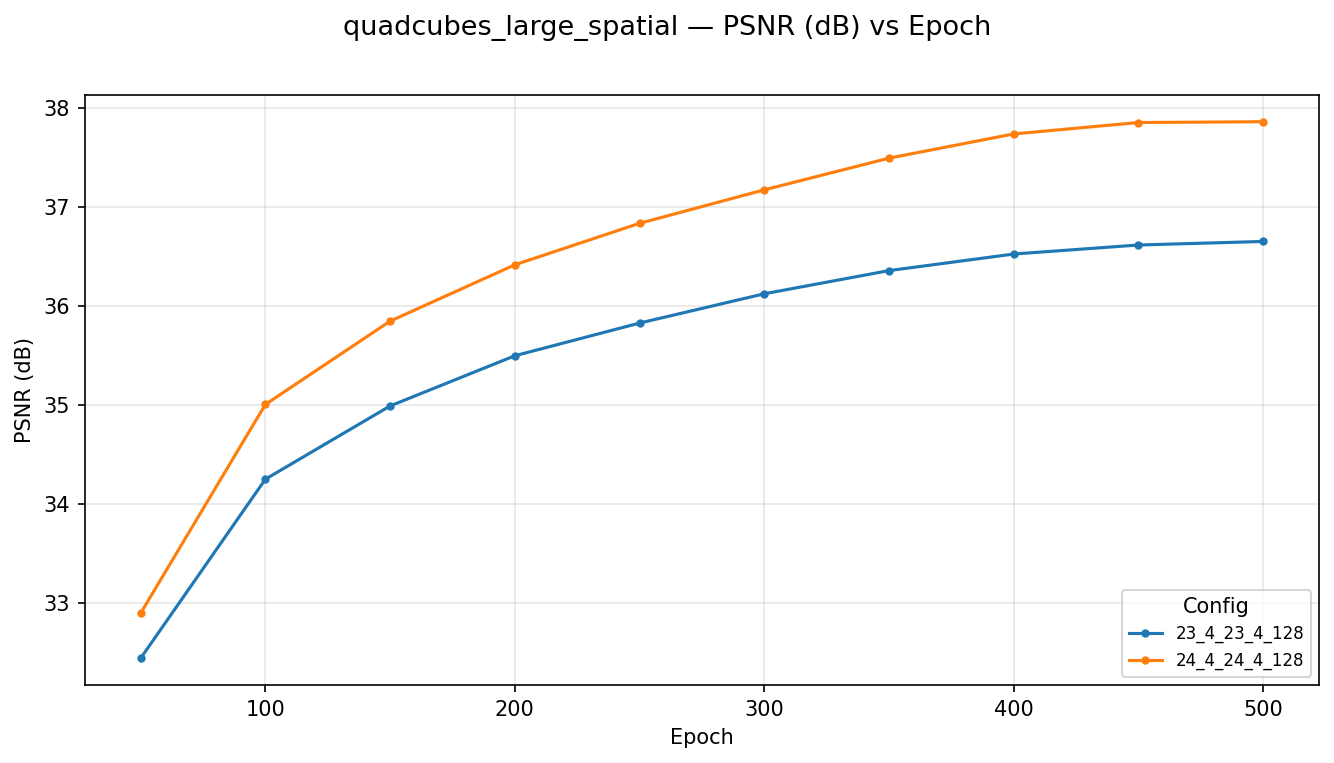
\includegraphics[width=1.1\textwidth]{psnr_arc/quadcubes_large_spatial_epoch_psnr.png}
    \end{adjustwidth}
    \caption{PSNR vs.\ epoch for QuadCubes with an enlarged spatial encoder (\texttt{xyz}) relative to the three temporal encoders. The smaller spatial-heavy config ($L=23$, $\log_2 T_\text{spatial}=23$, 20.1\,GB) reaches 36.65\,dB at epoch~500. The larger config ($L=24$, $\log_2 T=24$, 24.1\,GB) reaches 37.86\,dB at epoch~500.}
    \label{fig:spatial_heavy_epoch}
\end{figure}

\begin{figure}[htbp]
    \begin{adjustwidth}{-2.5cm}{-2.5cm}
    \centering
    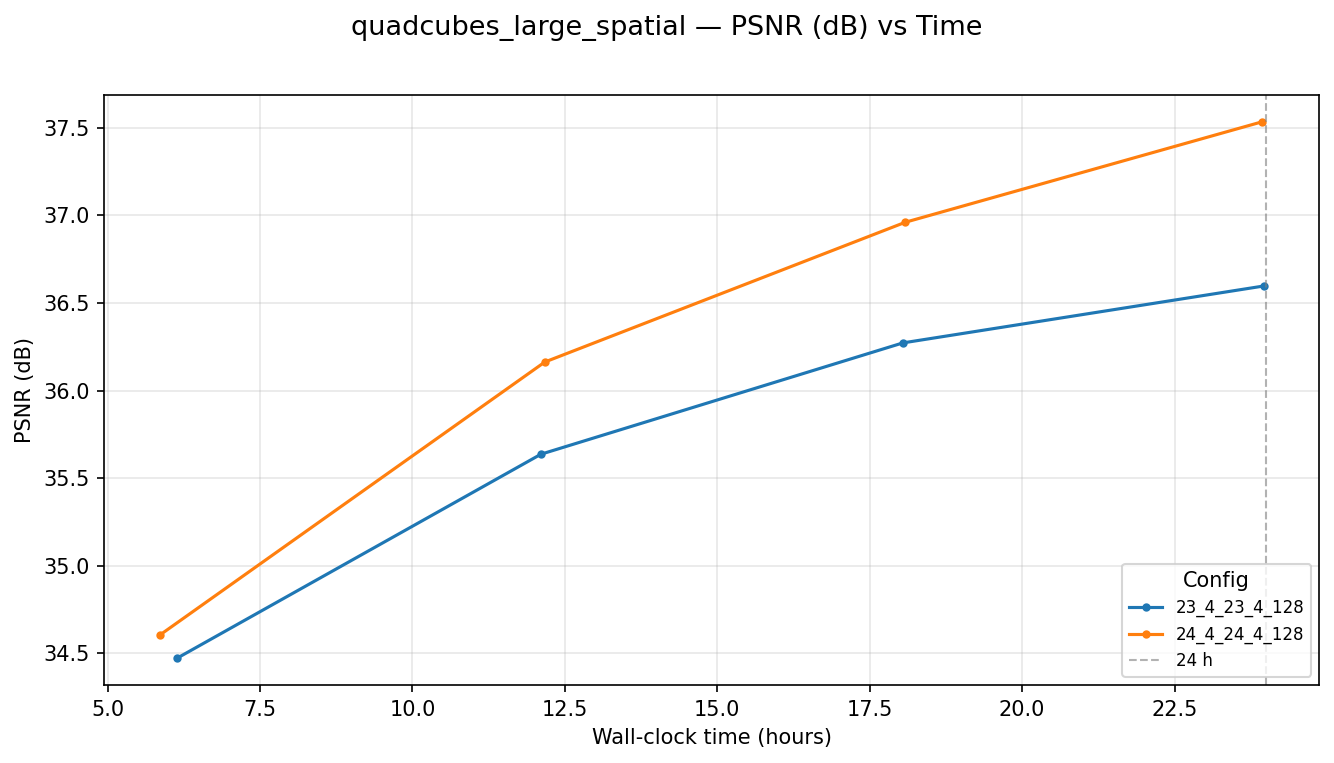
\includegraphics[width=1.1\textwidth]{psnr_arc/quadcubes_large_spatial_time_psnr.png}
    \end{adjustwidth}
    \caption{PSNR vs.\ wall-clock time for spatial-heavy QuadCubes configurations. At 24\,h the larger spatial-heavy configuration (24.1\,GB) achieves 37.53\,dB and the smaller (20.1\,GB) achieves 36.60\,dB, both exceeding the uniform baseline (44.8\,GB) while using less than half the VRAM.}
    \label{fig:spatial_heavy_time}
\end{figure}

\begin{figure}[htbp]
    \begin{adjustwidth}{-2.5cm}{-2.5cm}
    \centering
    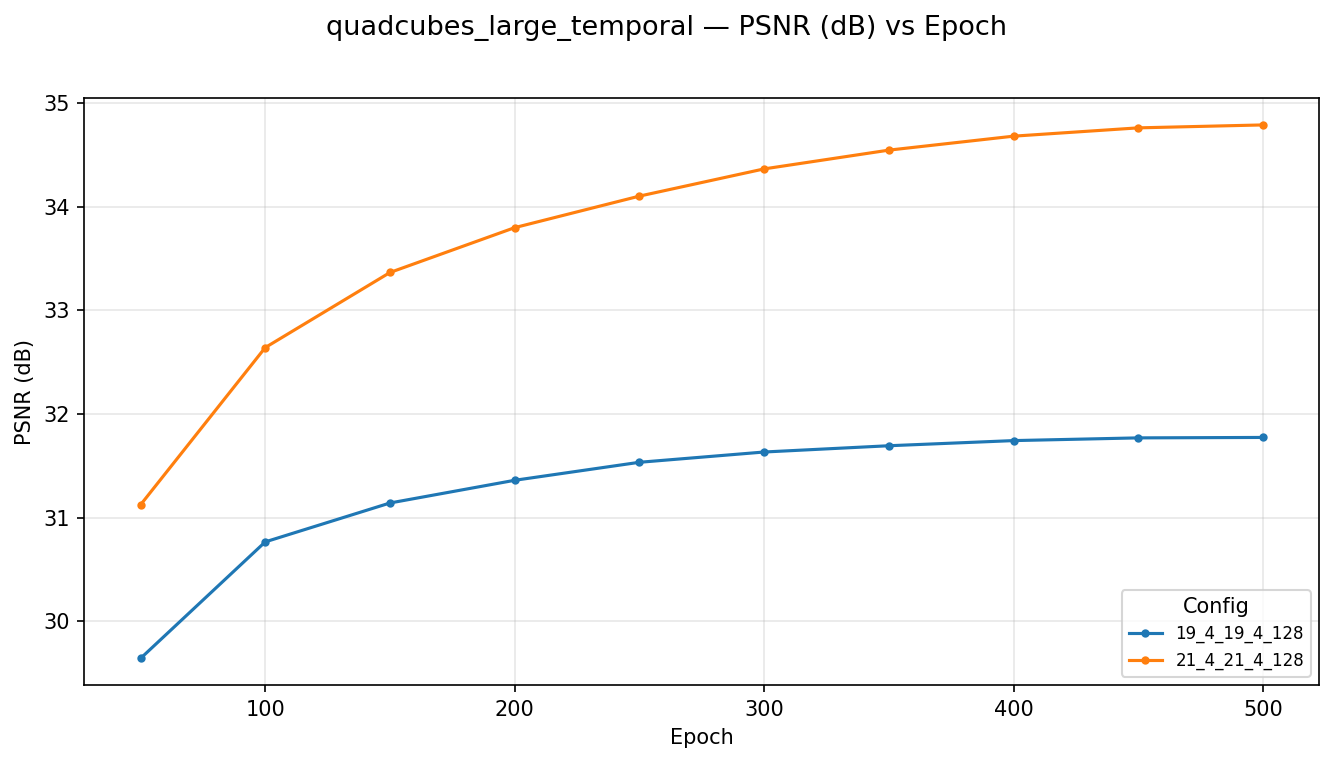
\includegraphics[width=1.1\textwidth]{psnr_arc/quadcubes_large_temporal_epoch_psnr.png}
    \end{adjustwidth}
    \caption{PSNR vs.\ epoch for QuadCubes with enlarged temporal encoders. Despite consuming 34--37\,GB VRAM, temporal-heavy configurations plateau well below the uniform baseline. At epoch~500 the larger temporal-heavy config (36.5\,GB) reaches 34.79\,dB versus the baseline's 36.47\,dB at 44.8\,GB; the smaller (34.4\,GB) only 31.77\,dB.}
    \label{fig:temporal_heavy_epoch}
\end{figure}

\begin{figure}[htbp]
    \begin{adjustwidth}{-2.5cm}{-2.5cm}
    \centering
    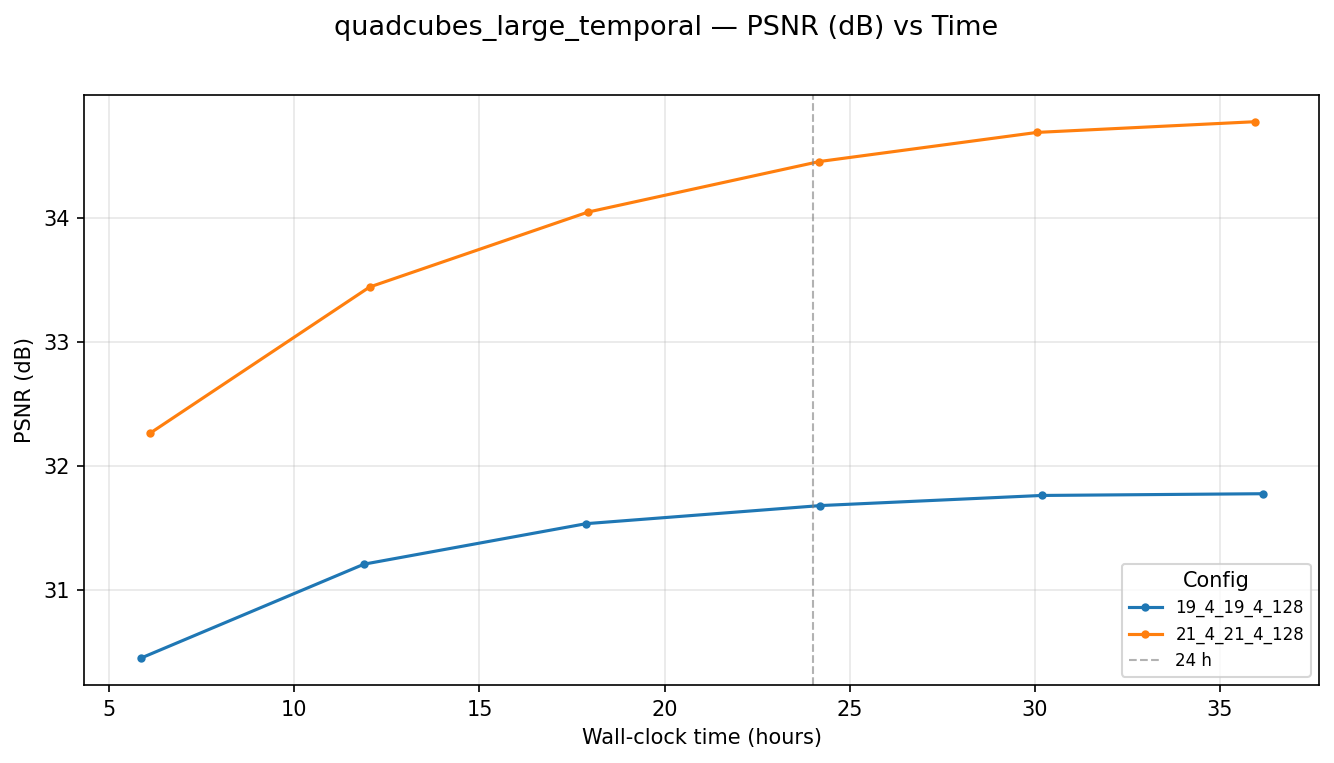
\includegraphics[width=1.1\textwidth]{psnr_arc/quadcubes_large_temporal_time_psnr.png}
    \end{adjustwidth}
    \caption{PSNR vs.\ wall-clock time for temporal-heavy QuadCubes configurations. At 24\,h the larger temporal-heavy config (36.5\,GB) reaches 34.46\,dB and the smaller (34.4\,GB) reaches 31.68\,dB, both substantially below the baseline despite comparable VRAM budgets.}
    \label{fig:temporal_heavy_time}
\end{figure}

The results confirm the asymmetry hypothesis. At 24\,h the smaller spatial-heavy configuration (20.1\,GB) achieves 36.60\,dB and the larger (24.1\,GB) achieves 37.53\,dB, both exceeding the baseline while using less than half the VRAM. Both spatial-heavy variants converge faster per epoch than the baseline because the reduced temporal encoder size lowers the per-step memory footprint and allows larger effective batch sizes.

A particularly striking result is that the smaller spatial-heavy configuration (Spatial-heavy A) uses an \emph{identical} $\texttt{xyz}$ encoder to the uniform baseline, differing only in that the three temporal encoders are reduced from $\log_2 T = 23$ to $\log_2 T = 21$. This is strictly a weaker model in temporal terms. Yet it outperforms the baseline by 0.71\,dB at less than half the VRAM. The temporal encoders in the original QuadCubes baseline were not contributing productive representational capacity — they were consuming memory and computation without returning a commensurate quality gain. Reducing the temporal encoders alone is enough to surpass the baseline. This finding directly motivates the architectural step to CombinedCubes. If simply scaling back the temporal hashmap size already yields improvement, reconsidering the temporal encoder design entirely and replacing large 3D hashed encoders with small collision-free 2D encoders should yield further gains, and the CombinedCubes results confirm that it does.

Temporal-heavy configurations tell the opposite story across both the epoch and the time plots. Despite consuming 34--37\,GB, the two temporal-heavy variants plateau well below the uniform baseline and show no sign of closing the gap with additional training. At 24\,h the larger temporal-heavy config (36.5\,GB) reaches only 34.46\,dB and the smaller (34.4\,GB) reaches 31.68\,dB. The epoch curves diverge early and maintain a stable offset, ruling out the possibility that the temporal-heavy models simply need more time. The quality deficit is structural. Additional hashmap capacity in the temporal encoders cannot represent spatial information the 2D temporal planes do not encode, and the MLP cannot recover spatial precision that the encoders never captured. Hashmap capacity allocated to the temporal encoders returns less quality per byte than the same capacity allocated to the spatial encoder, and increasing temporal capacity beyond the baseline allocation reduces reconstruction quality.

Figures~\ref{fig:quads_epoch}, \ref{fig:quads_time}, and \ref{fig:quads_vram} bring all four QuadCubes groups together in a single view. The pattern is unambiguous. In both the epoch and the wall-clock time plots, the two spatial-heavy configurations sit above the baseline and the smaller uniform configuration, while the two temporal-heavy configurations sit well below them. The VRAM-versus-quality plot makes the directional asymmetry concrete: moving budget from temporal to spatial encoders moves a configuration up and to the left on the Pareto plane (better quality, less memory), while moving budget to temporal encoders moves it down and to the right (worse quality, more memory). The baseline is not at the Pareto frontier even within the QuadCubes family. A smaller uniform configuration (22.1\,GB, \texttt{22\_4\_22\_4\_128}) matches the baseline quality at half the VRAM, and spatial-heavy reallocation without any change to the total parameter count produces a clear quality gain. The temporal encoders in the original QuadCubes design are over-provisioned, and correcting this within the QuadCubes architecture is already sufficient to surpass the baseline. CombinedCubes takes this structural insight further by redesigning the temporal encoders from the ground up rather than merely scaling them back.

\begin{figure}[H]
    \begin{adjustwidth}{-2.5cm}{-2.5cm}
    \centering
    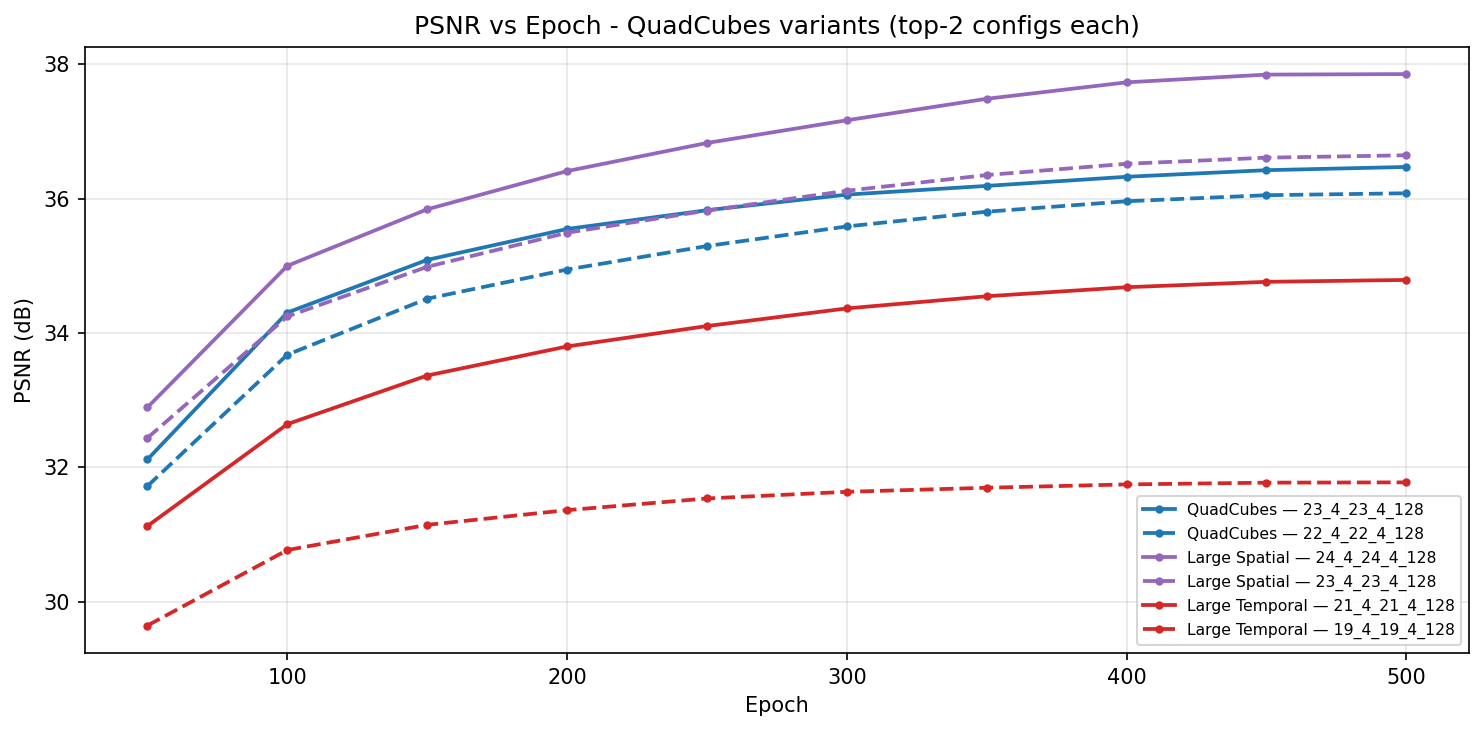
\includegraphics[width=1.1\textwidth]{top2/quad_psnr_epoch.png}
    \end{adjustwidth}
    \caption{PSNR vs.\ epoch for all QuadCubes configurations: the uniform baseline (\texttt{23\_4\_23\_4\_128}, 44.8\,GB), the smaller uniform variant (\texttt{22\_4\_22\_4\_128}, 23.1\,GB), both spatial-heavy variants, and both temporal-heavy variants. Spatial-heavy configurations sit consistently above the baseline and smaller uniform model; temporal-heavy configurations sit well below despite comparable or larger VRAM.}
    \label{fig:quads_epoch}
\end{figure}

\begin{figure}[H]
    \begin{adjustwidth}{-2.5cm}{-2.5cm}
    \centering
    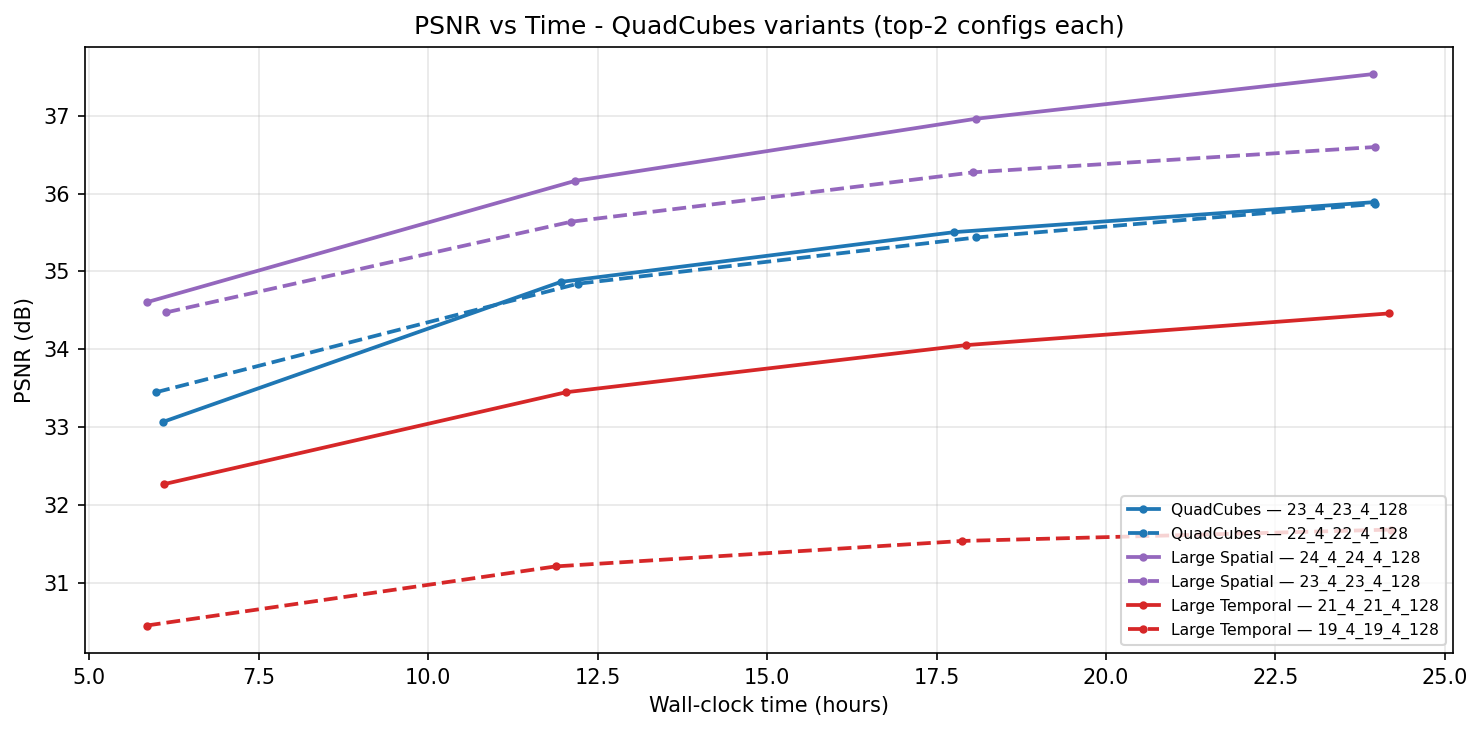
\includegraphics[width=1.1\textwidth]{top2/quad_psnr_time.png}
    \end{adjustwidth}
    \caption{PSNR vs.\ wall-clock time for all QuadCubes configurations. At 24\,h the spatial-heavy configs reach 36.60 and 37.53\,dB, both above the baseline's 35.89\,dB, while the temporal-heavy configs reach only 34.46 and 31.68\,dB. The ordering is stable throughout training — the asymmetry is not a convergence speed effect but a fundamental capacity allocation effect.}
    \label{fig:quads_time}
\end{figure}

\begin{figure}[H]
    \begin{adjustwidth}{-2.5cm}{-2.5cm}
    \centering
    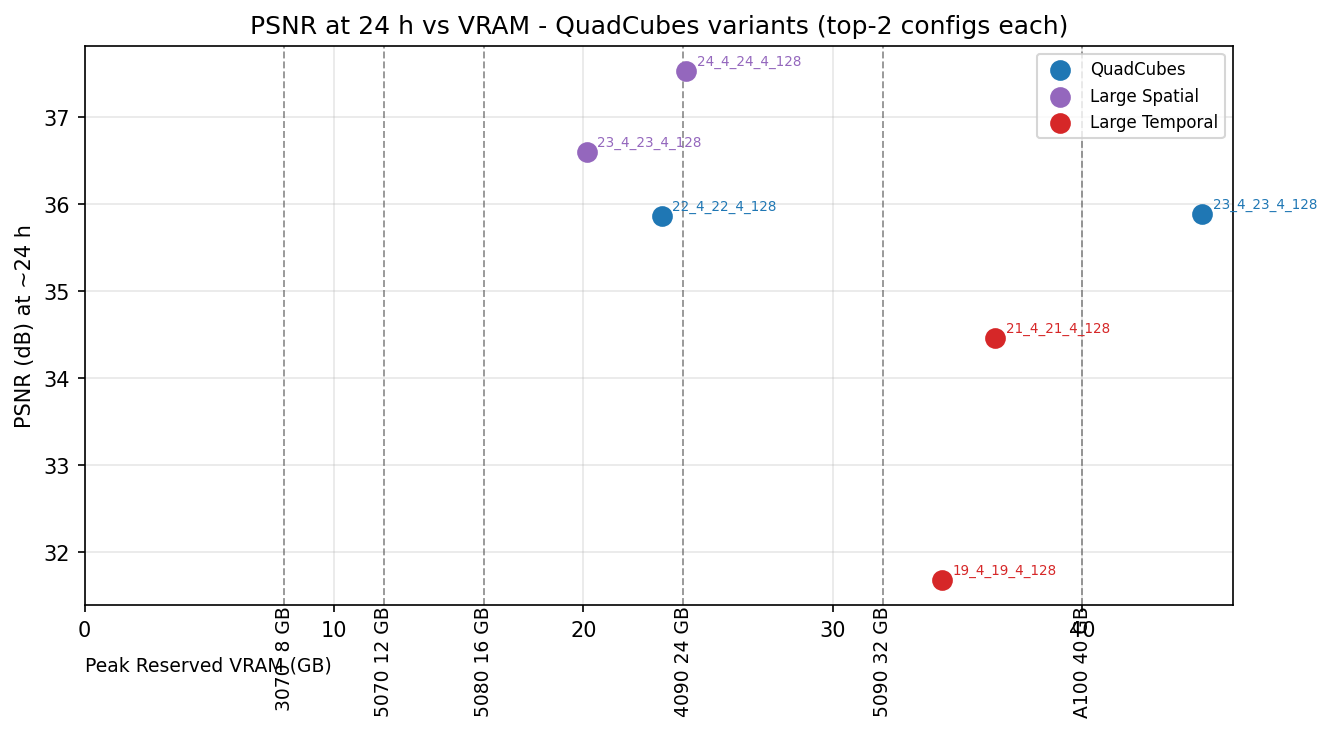
\includegraphics[width=1.1\textwidth]{top2/quad_vram.png}
    \end{adjustwidth}
    \caption{PSNR at 24\,h versus peak VRAM for all QuadCubes configurations. Spatial-heavy models occupy the upper-left region (higher quality, lower memory) relative to the baseline; temporal-heavy models occupy the lower-right region (lower quality, higher memory). The baseline is not at the Pareto frontier of its own architecture family. The direction of the asymmetry — spatial capacity is productive, temporal capacity is not — is the main finding motivating CombinedCubes.}
    \label{fig:quads_vram}
\end{figure}


\subsection{CombinedCubes}
\label{subsec:combinedcubes}

The non-uniform sizing experiments test the asymmetry hypothesis within the constraint that all encoders must have the same dimensionality. CombinedCubes removes that constraint and asks what the minimum viable temporal encoder is, given that temporal encoders appear to benefit from less capacity. The answer, following from the collision analysis in \cref{subsec:collision_dim_theory}, is a collision-free 2D encoder at $\log_2 T = 20$.

CombinedCubes uses one 3D spatial encoder (covering the $xyz$ coordinates) and three 2D temporal encoders covering the space-time pairs $xt$, $yt$, and $zt$ respectively. Figure~\ref{fig:combinedcubes_architecture} shows the architecture.

\begin{figure}[htbp]
    \centering
    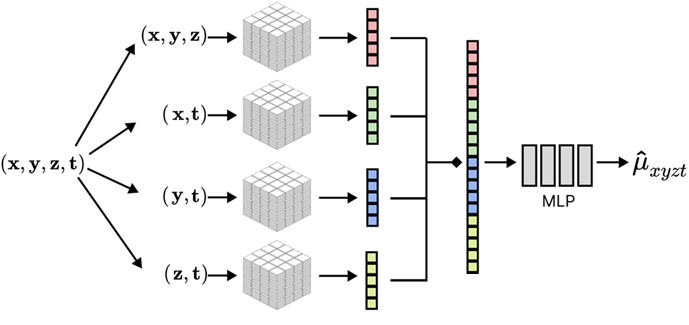
\includegraphics[width=0.80\textwidth]{arc_diagram/combinedcubes_diagram.png}
    \caption{The CombinedCubes architecture. One 3D hash encoder covers the spatial coordinates \texttt{xyz} and three collision-free 2D hash encoders cover the space-time pairs \texttt{xt}, \texttt{yt}, and \texttt{zt}. Features from all four encoders are concatenated and decoded by a shared MLP. The 2D temporal encoders require approximately 67\,\% less memory than equivalent 3D encoders while remaining collision-free at micro-CT resolutions.}
    \label{fig:combinedcubes_architecture}
\end{figure}

The encoder decomposition is:
%
\begin{equation}
    \muhat(\mathbf{r}, t) = \mathrm{MLP}_\Phi\!\Bigl(
        \bigl[
            \gamma_{xyz}(\mathbf{r};\,\theta_1),\;
            \gamma_{xt}(x,t;\,\theta_2),\;
            \gamma_{yt}(y,t;\,\theta_3),\;
            \gamma_{zt}(z,t;\,\theta_4)
        \bigr]
    \Bigr).
    \label{eq:combinedcubes_forward}
\end{equation}
%
This design separates the representation of the static pore geometry from the representation of temporal change along each spatial axis. The spatial encoder handles the time-invariant structure with the same collision load as a standard QuadCubes \texttt{xyz} encoder. The three 2D temporal encoders, each collision-free at $\log_2 T = 20$, capture how attenuation co-varies with time along a single spatial direction. The 2D encoders do not need to resolve the full 3D spatial structure. They only need to encode how each spatial slice evolves over time, which is a lower-dimensional and lower-frequency signal.

The practical consequence is a memory reduction of approximately 67\%. Three 2D encoders at $\log_2 T = 20$ with $L = 16$ and $F = 4$ occupy approximately 384\,MB total, compared to 3.9\,GB for three 3D encoders at $\log_2 T = 23$ with $L = 23$ and $F = 4$. Adding the spatial encoder at approximately 1.3\,GB gives a total hash table footprint of approximately 1.7\,GB for CombinedCubes versus 5.2\,GB for the baseline QuadCubes.

\begin{figure}[htbp]
    \begin{adjustwidth}{-2cm}{-2cm}
    \centering
    \begin{subfigure}[b]{0.45\textwidth}
        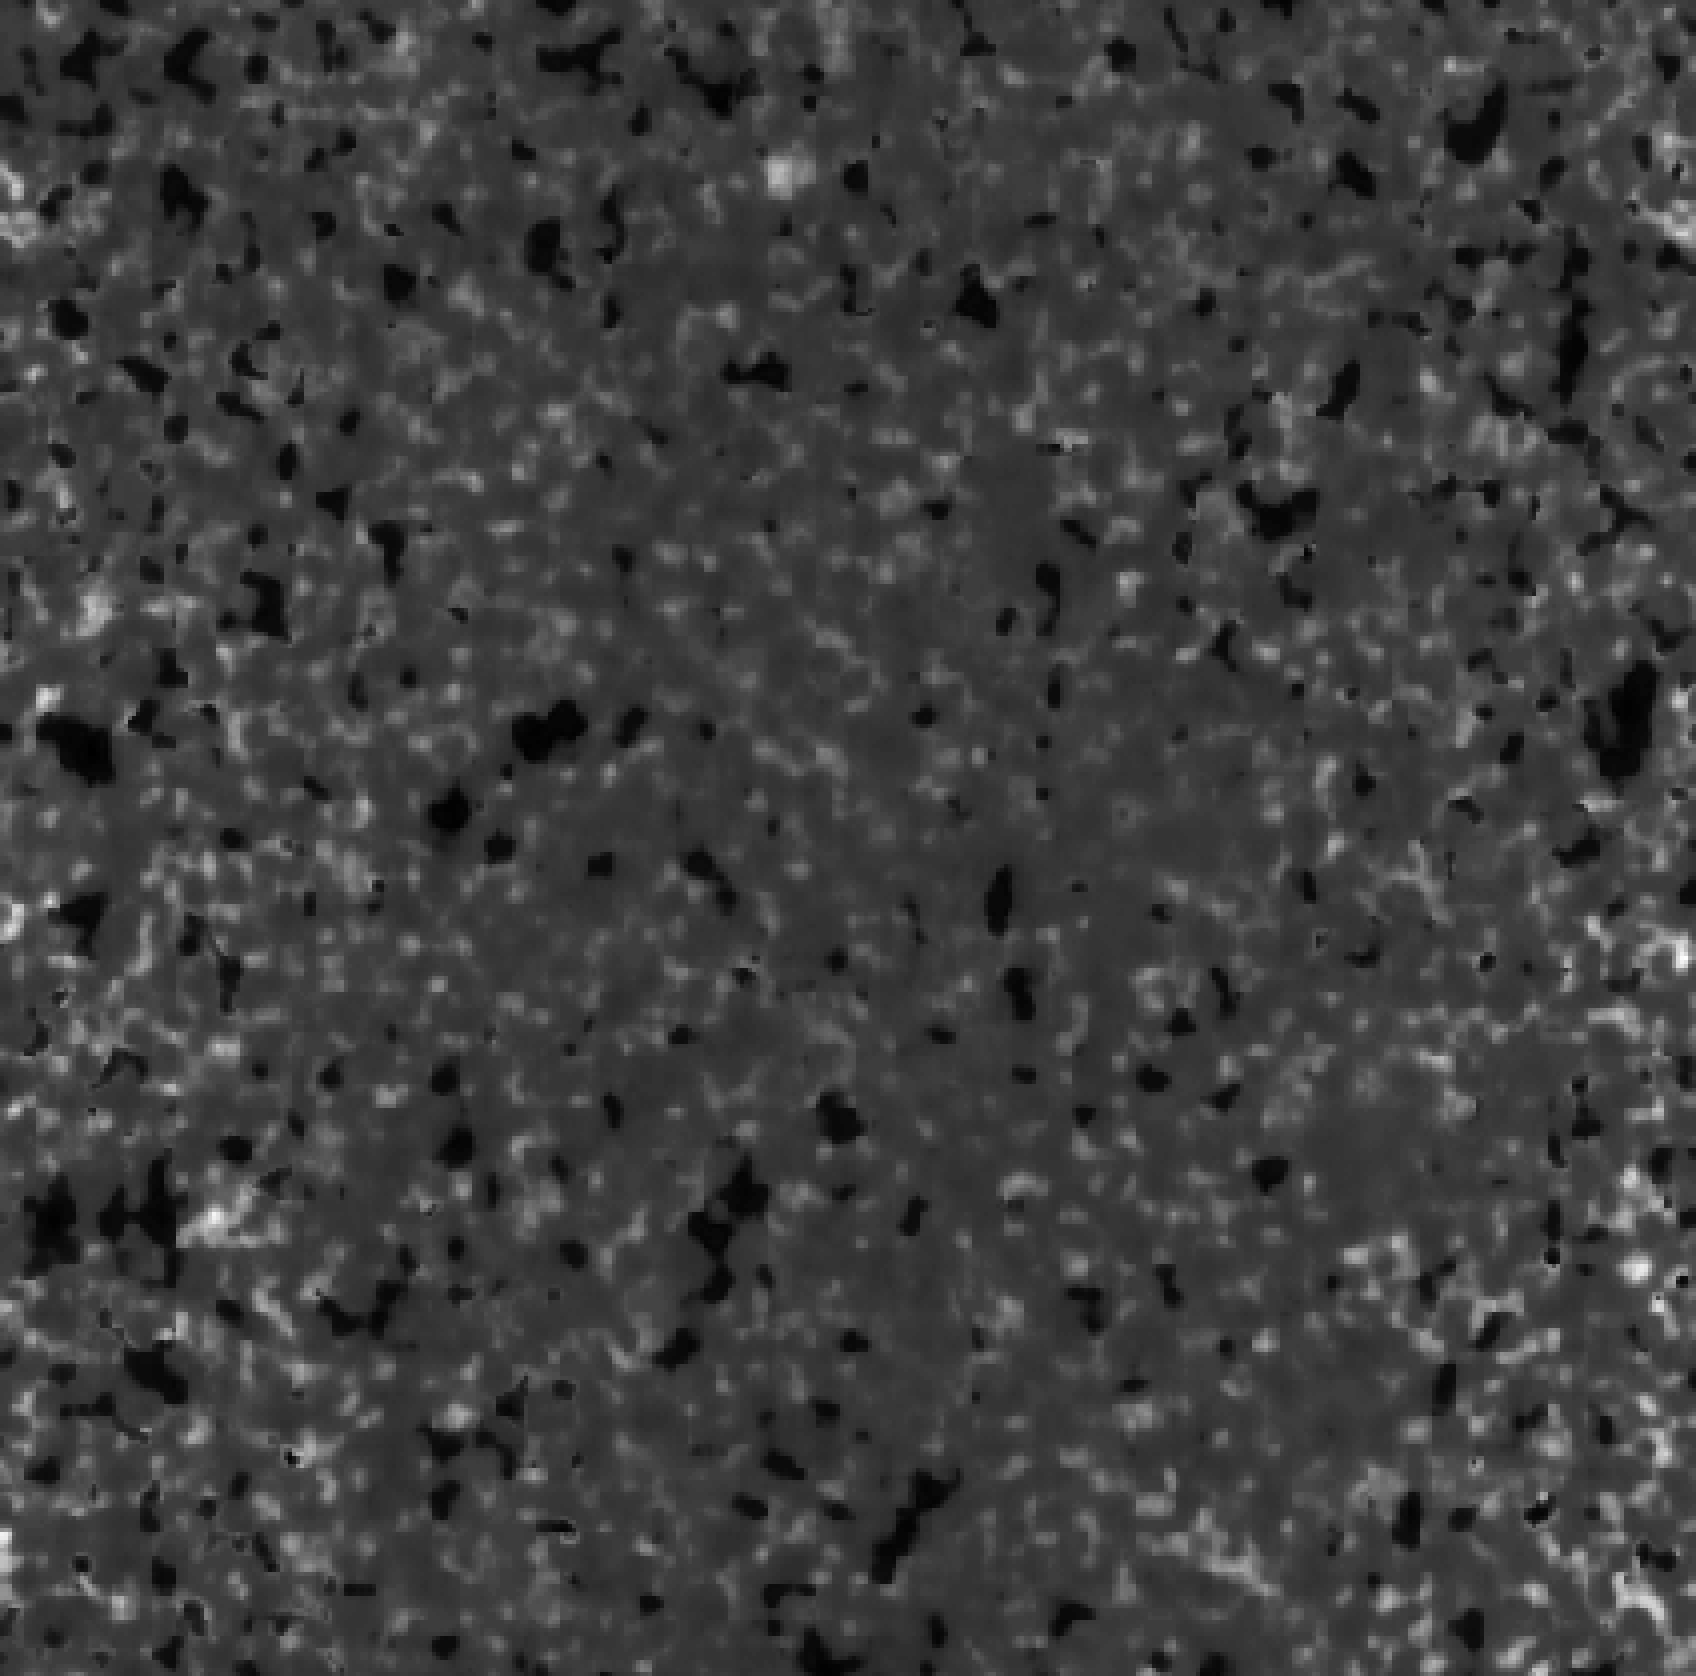
\includegraphics[width=\textwidth]{combinedcube_150epoch.png}
        \caption{CombinedCubes}
    \end{subfigure}
    \hspace{0.2cm}
    \begin{subfigure}[b]{0.45\textwidth}
        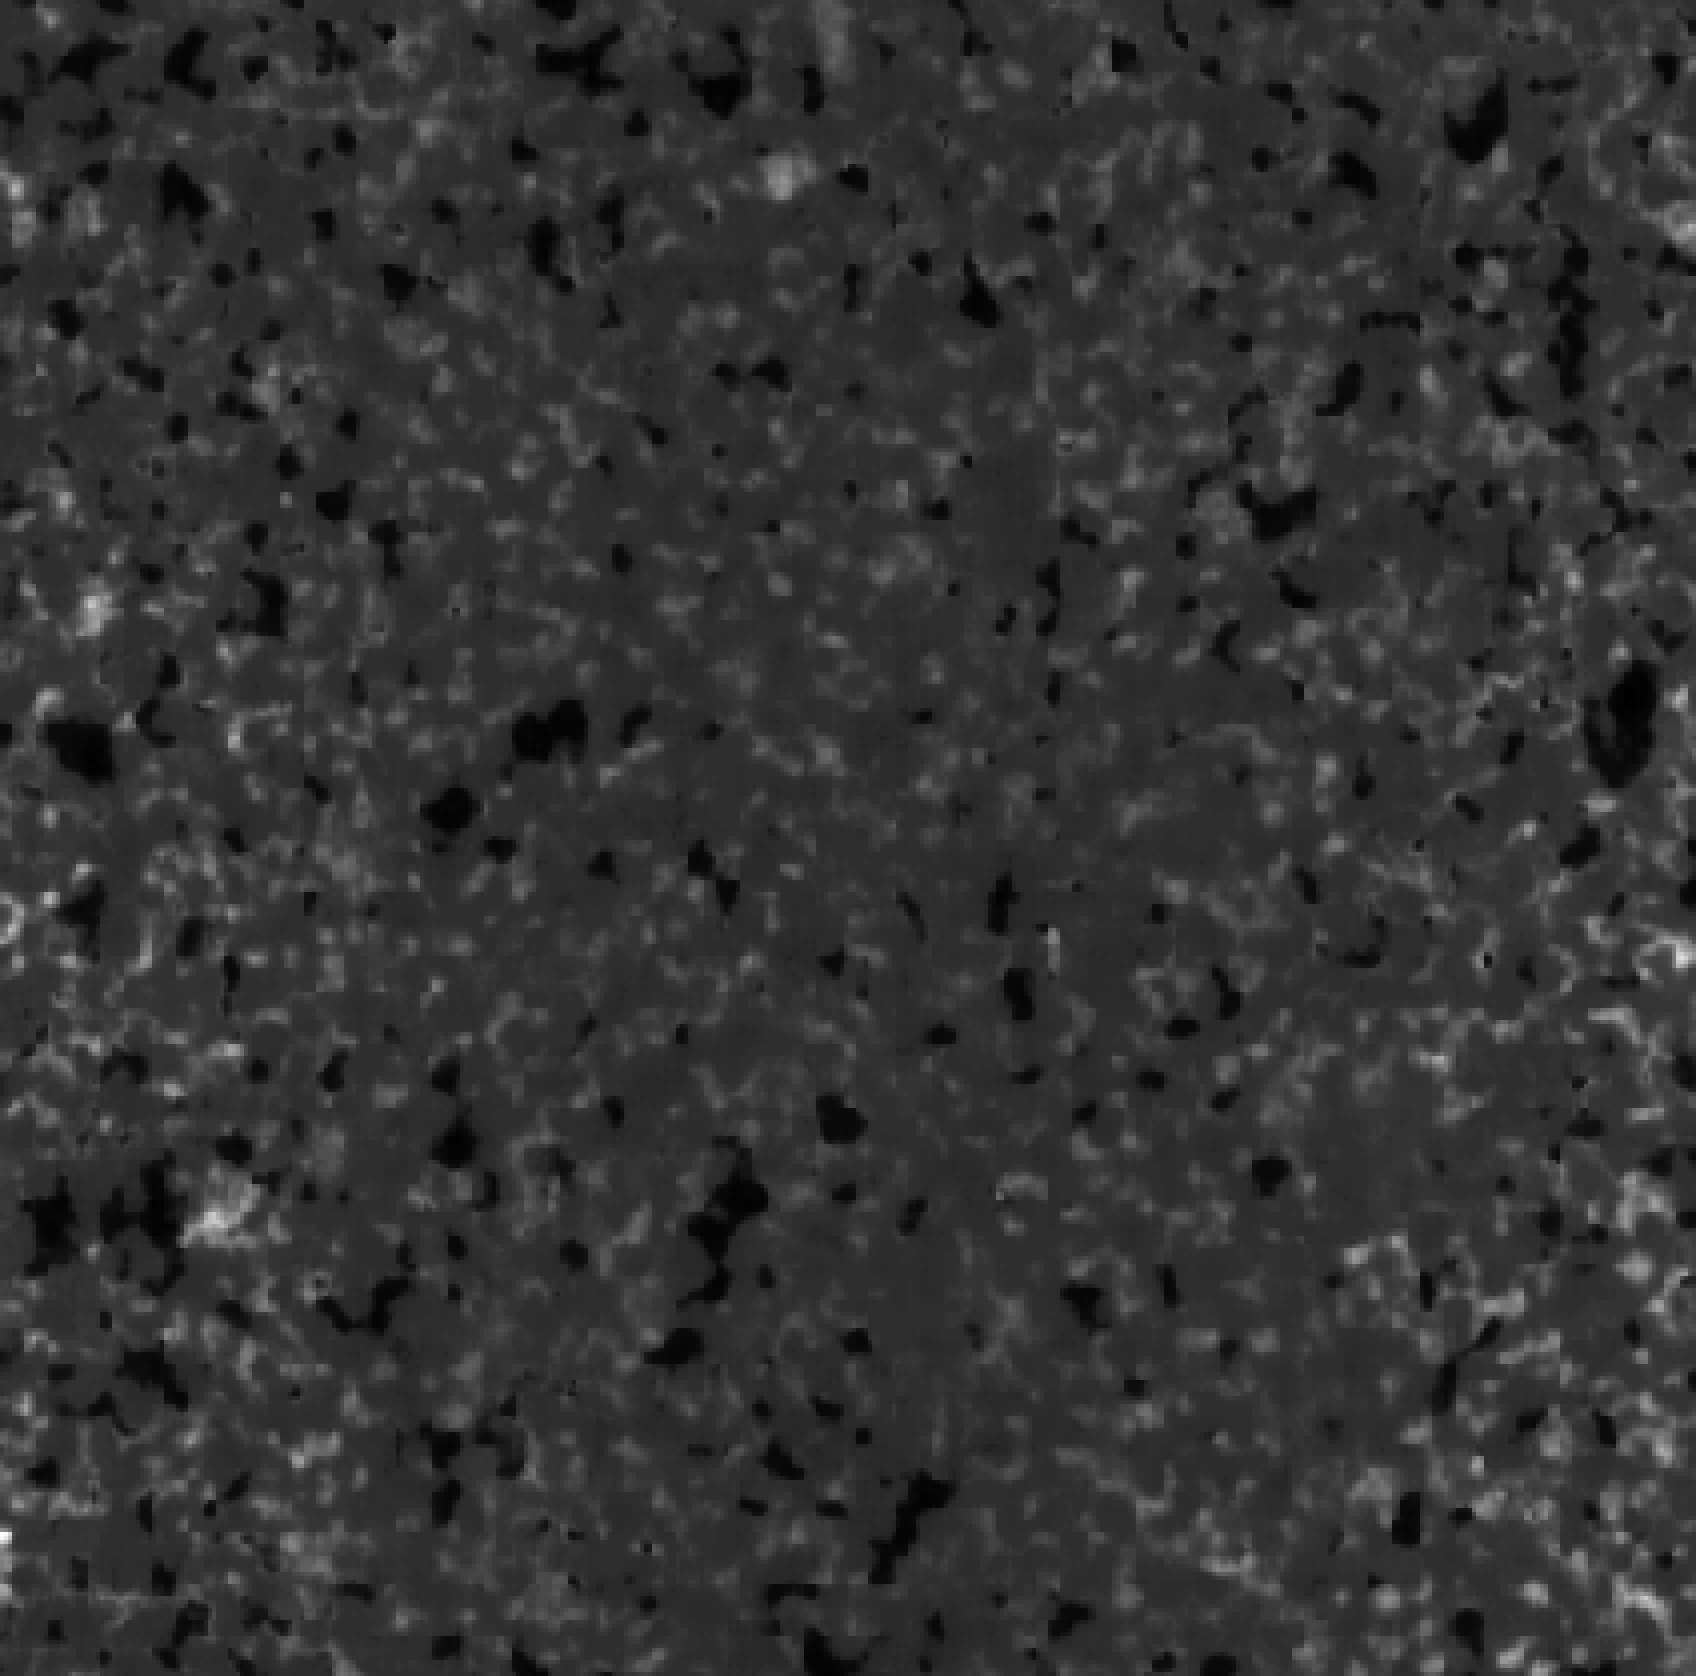
\includegraphics[width=\textwidth]{quadcube_150epoch.png}
        \caption{QuadCubes (baseline)}
    \end{subfigure}
    \end{adjustwidth}
    \caption{Reconstruction slices from CombinedCubes and QuadCubes after 150 epochs with the same baseline MLP configuration. The temporal encoders in CombinedCubes use $\log_2 T = 20$ (collision-free 2D grids). The slice is taken from the upper right corner of the Bentheimer dataset at the final timestep, where the brine front has reached the top of the sample.}
    \label{fig:combinedcubes_reconstruction}
\end{figure}

\begin{figure}[htbp]
    \begin{adjustwidth}{-2.5cm}{0cm}
    \centering
    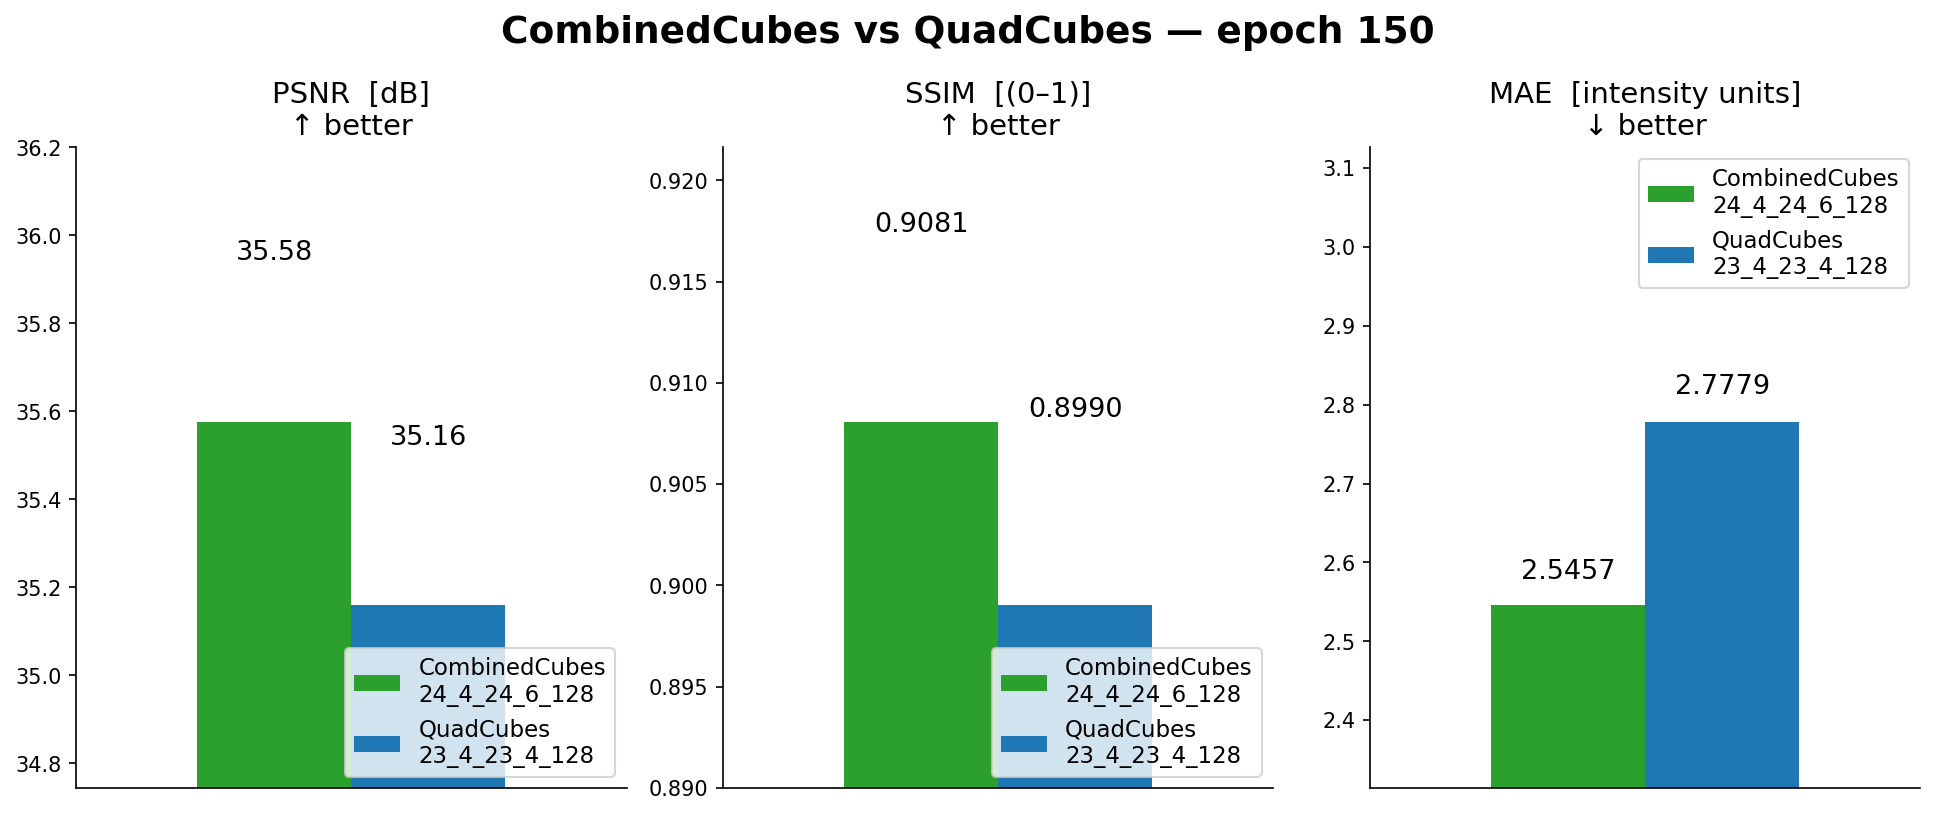
\includegraphics[width=1.1\textwidth]{cc_qc_comp.png}
    \end{adjustwidth}
    \caption{PSNR, SSIM, and MAE for CombinedCubes and QuadCubes at 150 epochs. CombinedCubes: PSNR 35.58\,dB, SSIM 0.908, MAE 2.55. QuadCubes: PSNR 35.16\,dB, SSIM 0.899, MAE 2.78.}
    \label{fig:combinedcubes_quality}
\end{figure}

\begin{figure}[htbp]
    \begin{adjustwidth}{-2.5cm}{-2.5cm}
    \centering
    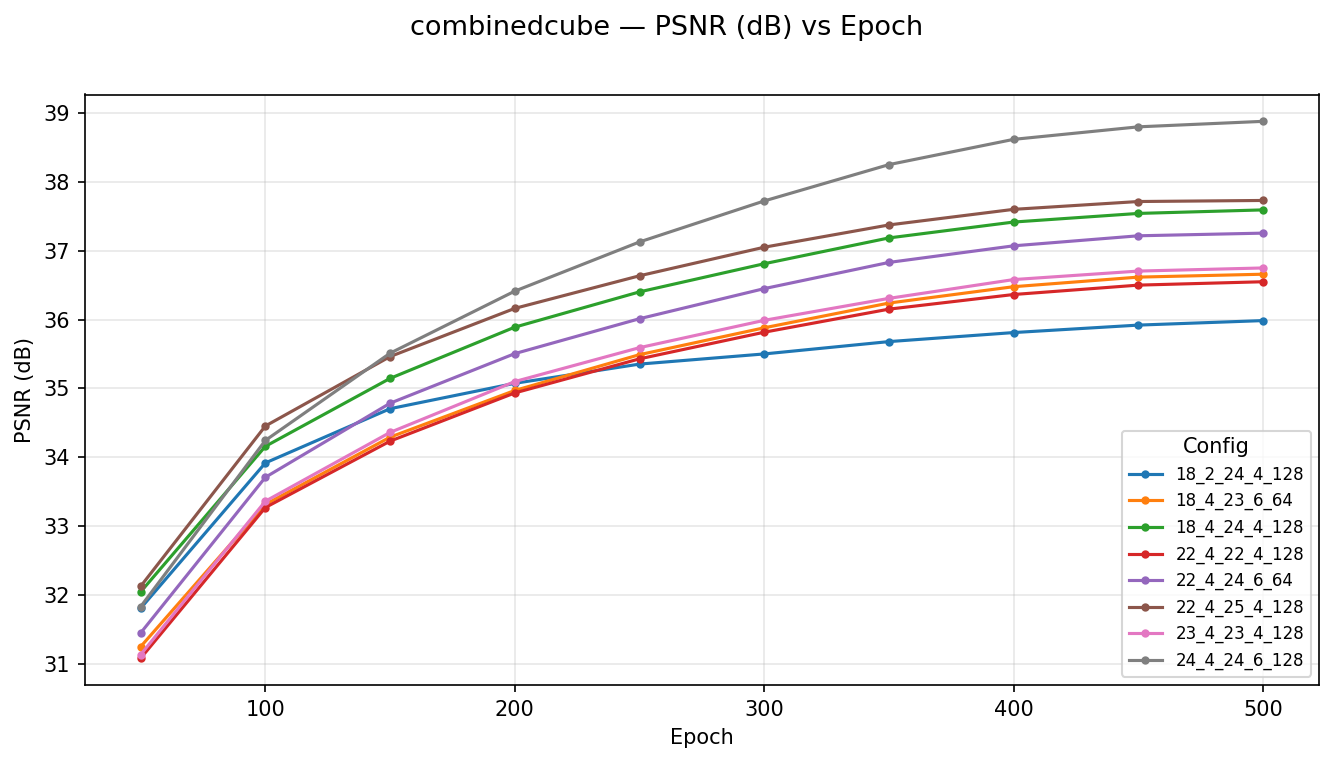
\includegraphics[width=1.1\textwidth]{psnr_arc/combinedcube_epoch_psnr.png}
    \end{adjustwidth}
    \caption{PSNR vs.\ epoch for the eight representative CombinedCubes configurations shown here. The best-performing configuration (\texttt{24\_4\_24\_6\_128}, 24.3\,GB) reaches 38.88\,dB at epoch~500, 2.41\,dB above the QuadCubes baseline (36.47\,dB, 44.8\,GB). Configurations with $F=2$ (the \texttt{18\_2\_} and \texttt{20\_2\_} prefix families) underperform relative to $F=4$ equivalents at comparable VRAM, indicating that halving the feature dimension in the split-encoder context degrades quality unlike in the uniform QuadCubes sweep.}
    \label{fig:combinedcubes_epoch}
\end{figure}

\begin{figure}[htbp]
    \begin{adjustwidth}{-2.5cm}{-2.5cm}
    \centering
    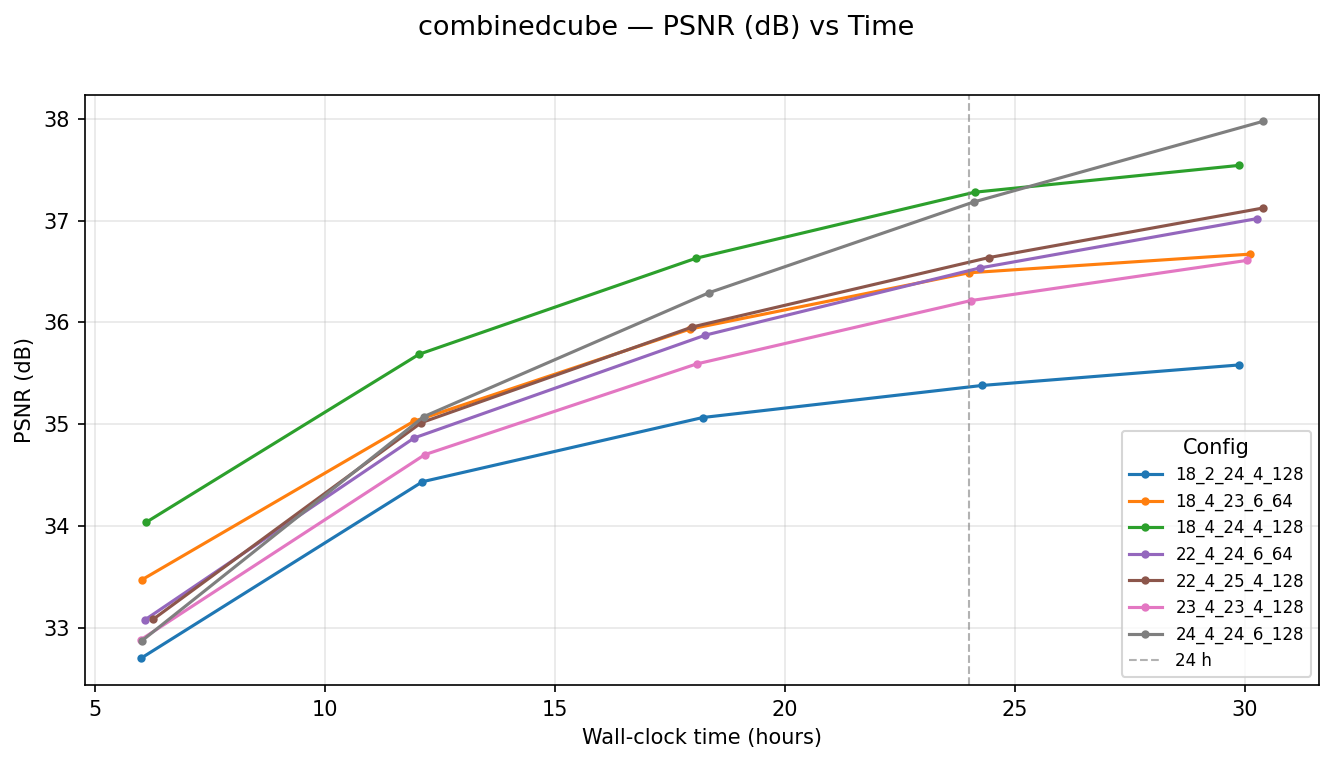
\includegraphics[width=1.1\textwidth]{psnr_arc/combinedcube_time_psnr.png}
    \end{adjustwidth}
    \caption{PSNR vs.\ wall-clock time for the eight representative CombinedCubes configurations. At 24\,h the best configurations are \texttt{18\_4\_24\_4\_128} (18.3\,GB) at 37.28\,dB and \texttt{24\_4\_24\_6\_128} (24.3\,GB) at 37.18\,dB, both substantially exceeding the QuadCubes baseline's 35.89\,dB. The $F=2$ configuration \texttt{18\_2\_24\_4\_128} (19.5\,GB) reaches only 35.38\,dB at 24\,h, below the baseline, confirming that halving the feature dimension in this context is counterproductive.}
    \label{fig:combinedcubes_time}
\end{figure}

The eight CombinedCubes configurations shown here were selected from a larger experimental set to best illustrate the range of performance across different memory, training time, and quality trade-offs.

Figures~\ref{fig:combinedcubes_reconstruction} and~\ref{fig:combinedcubes_quality} show the initial 150-epoch comparison. At this checkpoint CombinedCubes outperforms QuadCubes on all three metrics: PSNR 35.58 versus 35.16\,dB ($+0.42$\,dB), SSIM 0.908 versus 0.899 ($+0.009$), and MAE 2.55 versus 2.78 ($-0.23$). The differences are modest, as expected at an early checkpoint, but they are consistent in direction. Importantly, CombinedCubes reaches 150 epochs faster than QuadCubes because its smaller temporal encoders reduce per-step computation, meaning the quality advantage visible in these plots was achieved in less wall-clock time. Over the full training run (Figures~\ref{fig:combinedcubes_epoch} and \ref{fig:combinedcubes_time}), the advantage deepens. At epoch~500 the best CombinedCubes configuration (\texttt{24\_4\_24\_6\_128}, 24.3\,GB) reaches 38.88\,dB PSNR, SSIM 0.945, and MAE 1.8, compared to the QuadCubes baseline's 36.47\,dB, SSIM 0.921, and MAE 2.4. At the 24-hour wall-clock mark, \texttt{18\_4\_24\_4\_128} (18.3\,GB) achieves 37.28\,dB PSNR, SSIM 0.926, and MAE 2.1, a gain of $+1.39$\,dB over the baseline at 59\% less VRAM. The \texttt{24\_4\_24\_6\_128} configuration (24.3\,GB) achieves 37.18\,dB at 24\,h.

A notable pattern in the CombinedCubes results is that configurations with $F=2$ (halved feature dimension) consistently underperform relative to $F=4$ equivalents at comparable VRAM. The \texttt{18\_2\_24\_4\_128} configuration (19.5\,GB, $F=2$ on temporal encoders) reaches only 35.38\,dB at 24\,h, $0.51$\,dB below the QuadCubes baseline despite consuming similar memory. This contrasts with the QuadCubes-uniform features sweep, which found $F=2$ nearly as capable as $F=4$. The difference arises because in the split-encoder context the temporal encoders are already small and collision-free, reducing their feature dimension further removes representational capacity that is actually needed, whereas in the over-provisioned QuadCubes baseline, halving $F$ eliminated redundancy without harm.

Decoder depth has a modest and configuration-dependent effect. The best-performing configuration at the 24-hour mark uses 4 hidden layers, while the best epoch-500 result comes from a 6-layer configuration. CombinedCubes separates the spatial and temporal encoders more cleanly than QuadCubes, so the MLP receives less redundant information and may benefit from slightly more capacity to integrate it. However, 4 hidden layers are sufficient for the strongest time-budget results in practice.

\subsection{\MixedCubes}
\label{subsec:mixedcubes}

\begin{figure}[htbp]
    \centering
    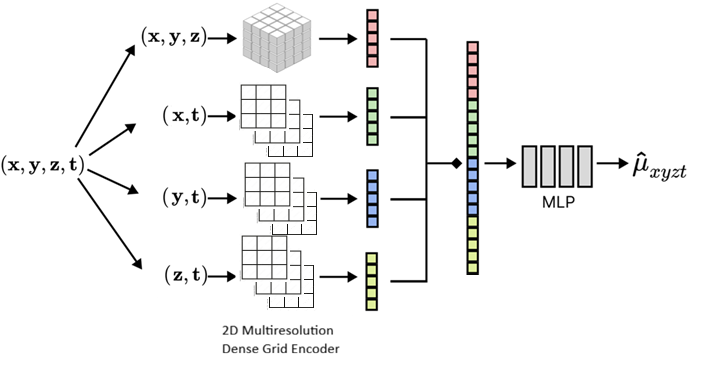
\includegraphics[width=0.80\textwidth]{arc_diagram/mixedcubes_diagram.png}
    \caption{The \MixedCubes{} architecture. One 3D multiresolution hash encoder covers the spatial coordinates \texttt{xyz} and three fully dense 2D grids cover the space-time pairs \texttt{xt}, \texttt{yt}, and \texttt{zt}. Dense grids guarantee an exact coordinate-to-feature correspondence with no hash collisions by construction. Features from all four encoders are concatenated and decoded by a shared MLP.}
    \label{fig:mixedcubes_architecture}
\end{figure}

\begin{figure}[htbp]
    \begin{adjustwidth}{-2cm}{-2cm}
    \centering
    \begin{subfigure}[b]{0.45\textwidth}
        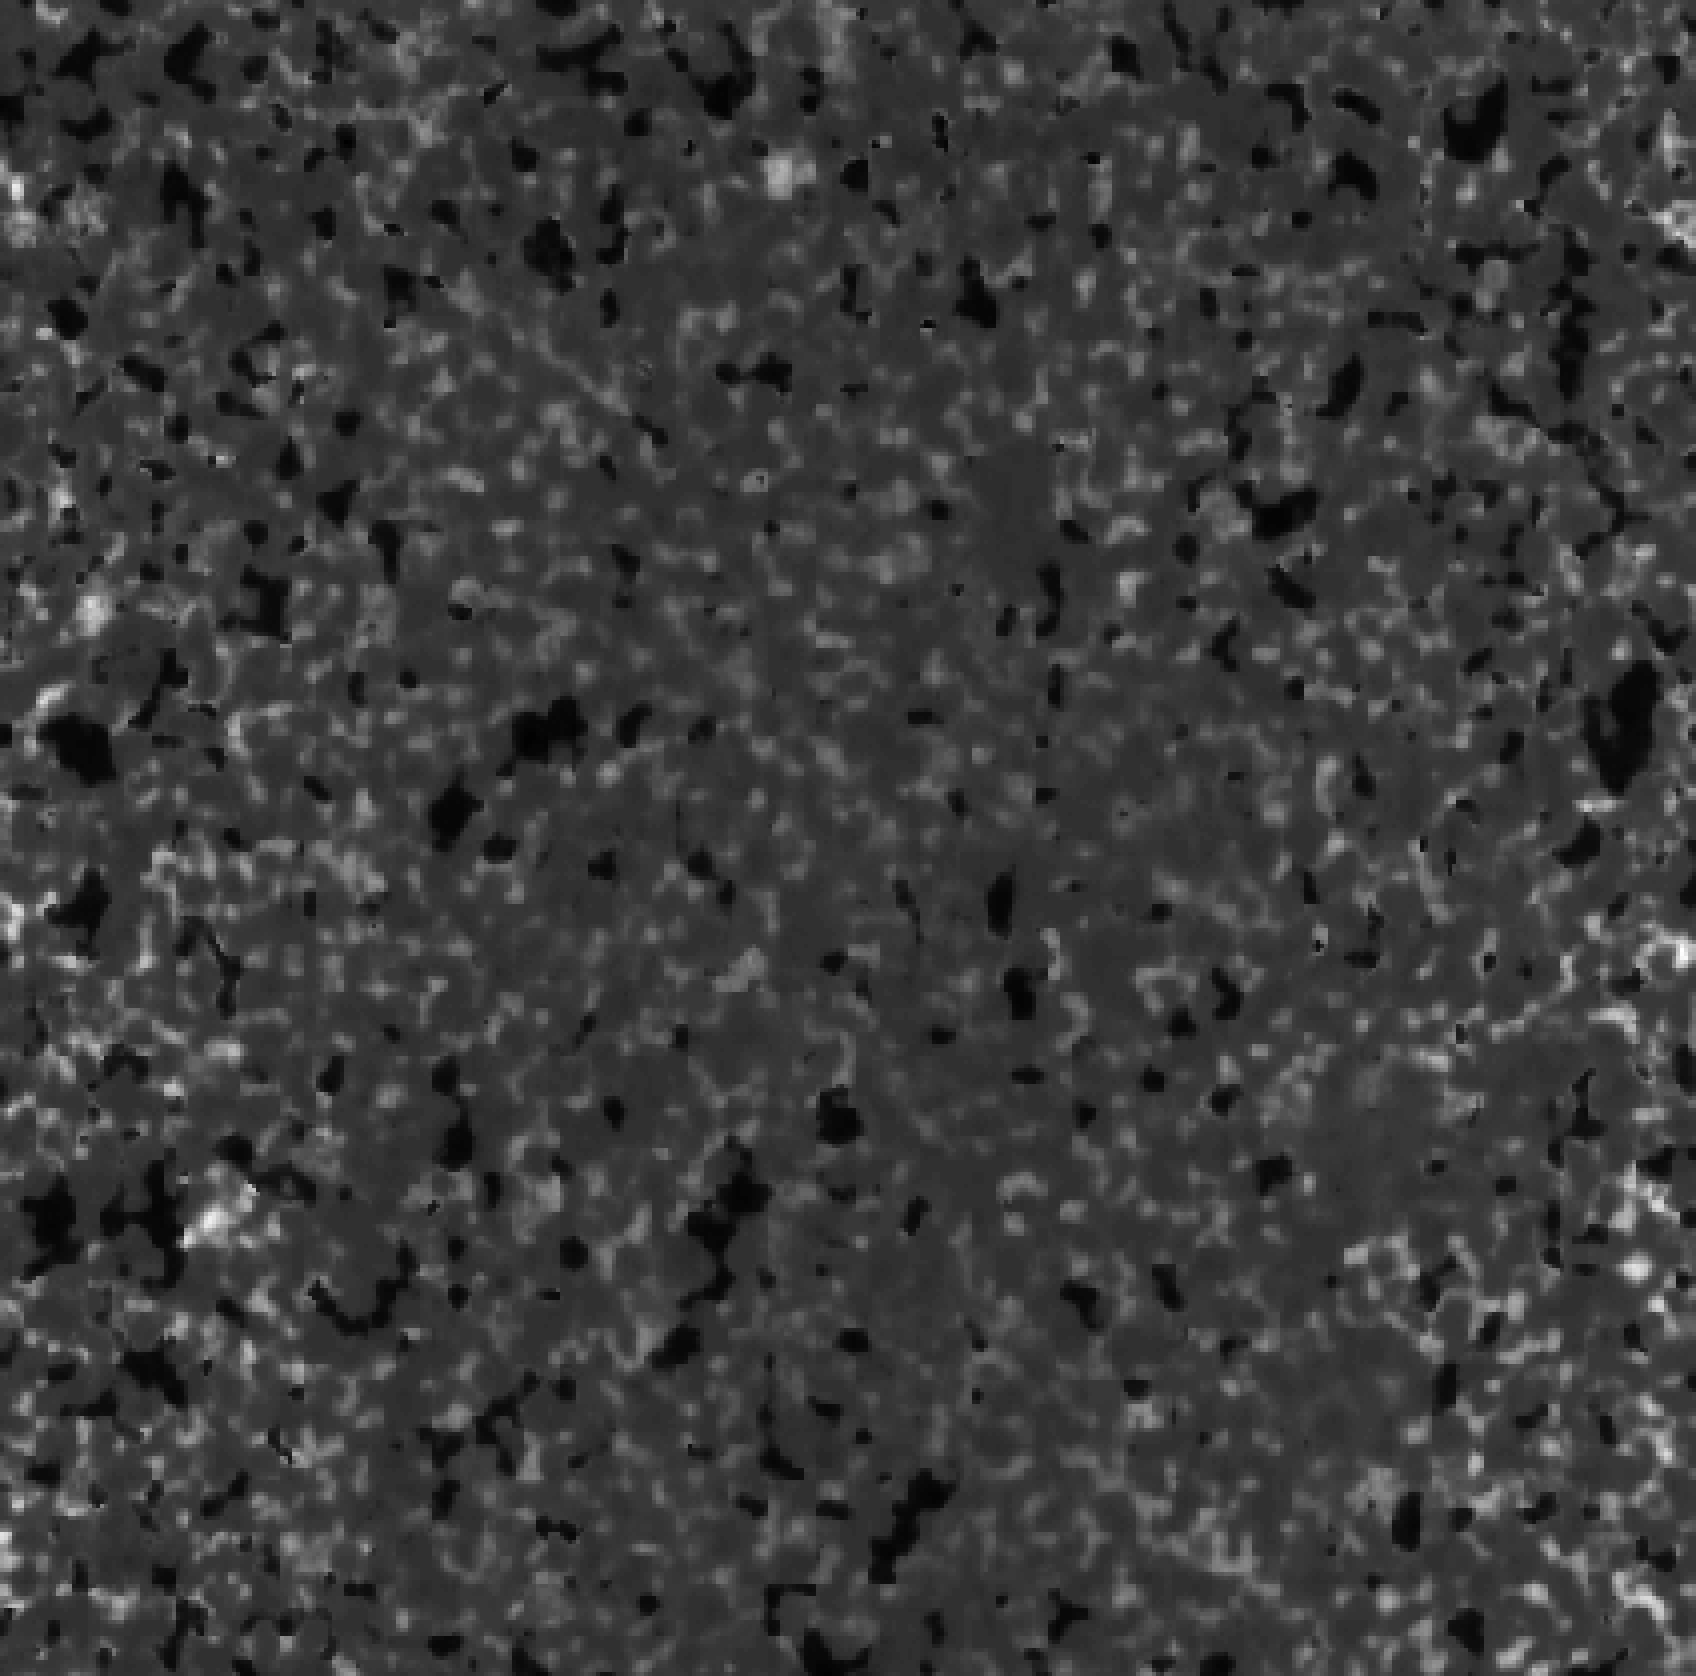
\includegraphics[width=\textwidth]{compairson.png}
        \caption{Ground truth}
    \end{subfigure}
    \hspace{0.2cm}
    \begin{subfigure}[b]{0.45\textwidth}
        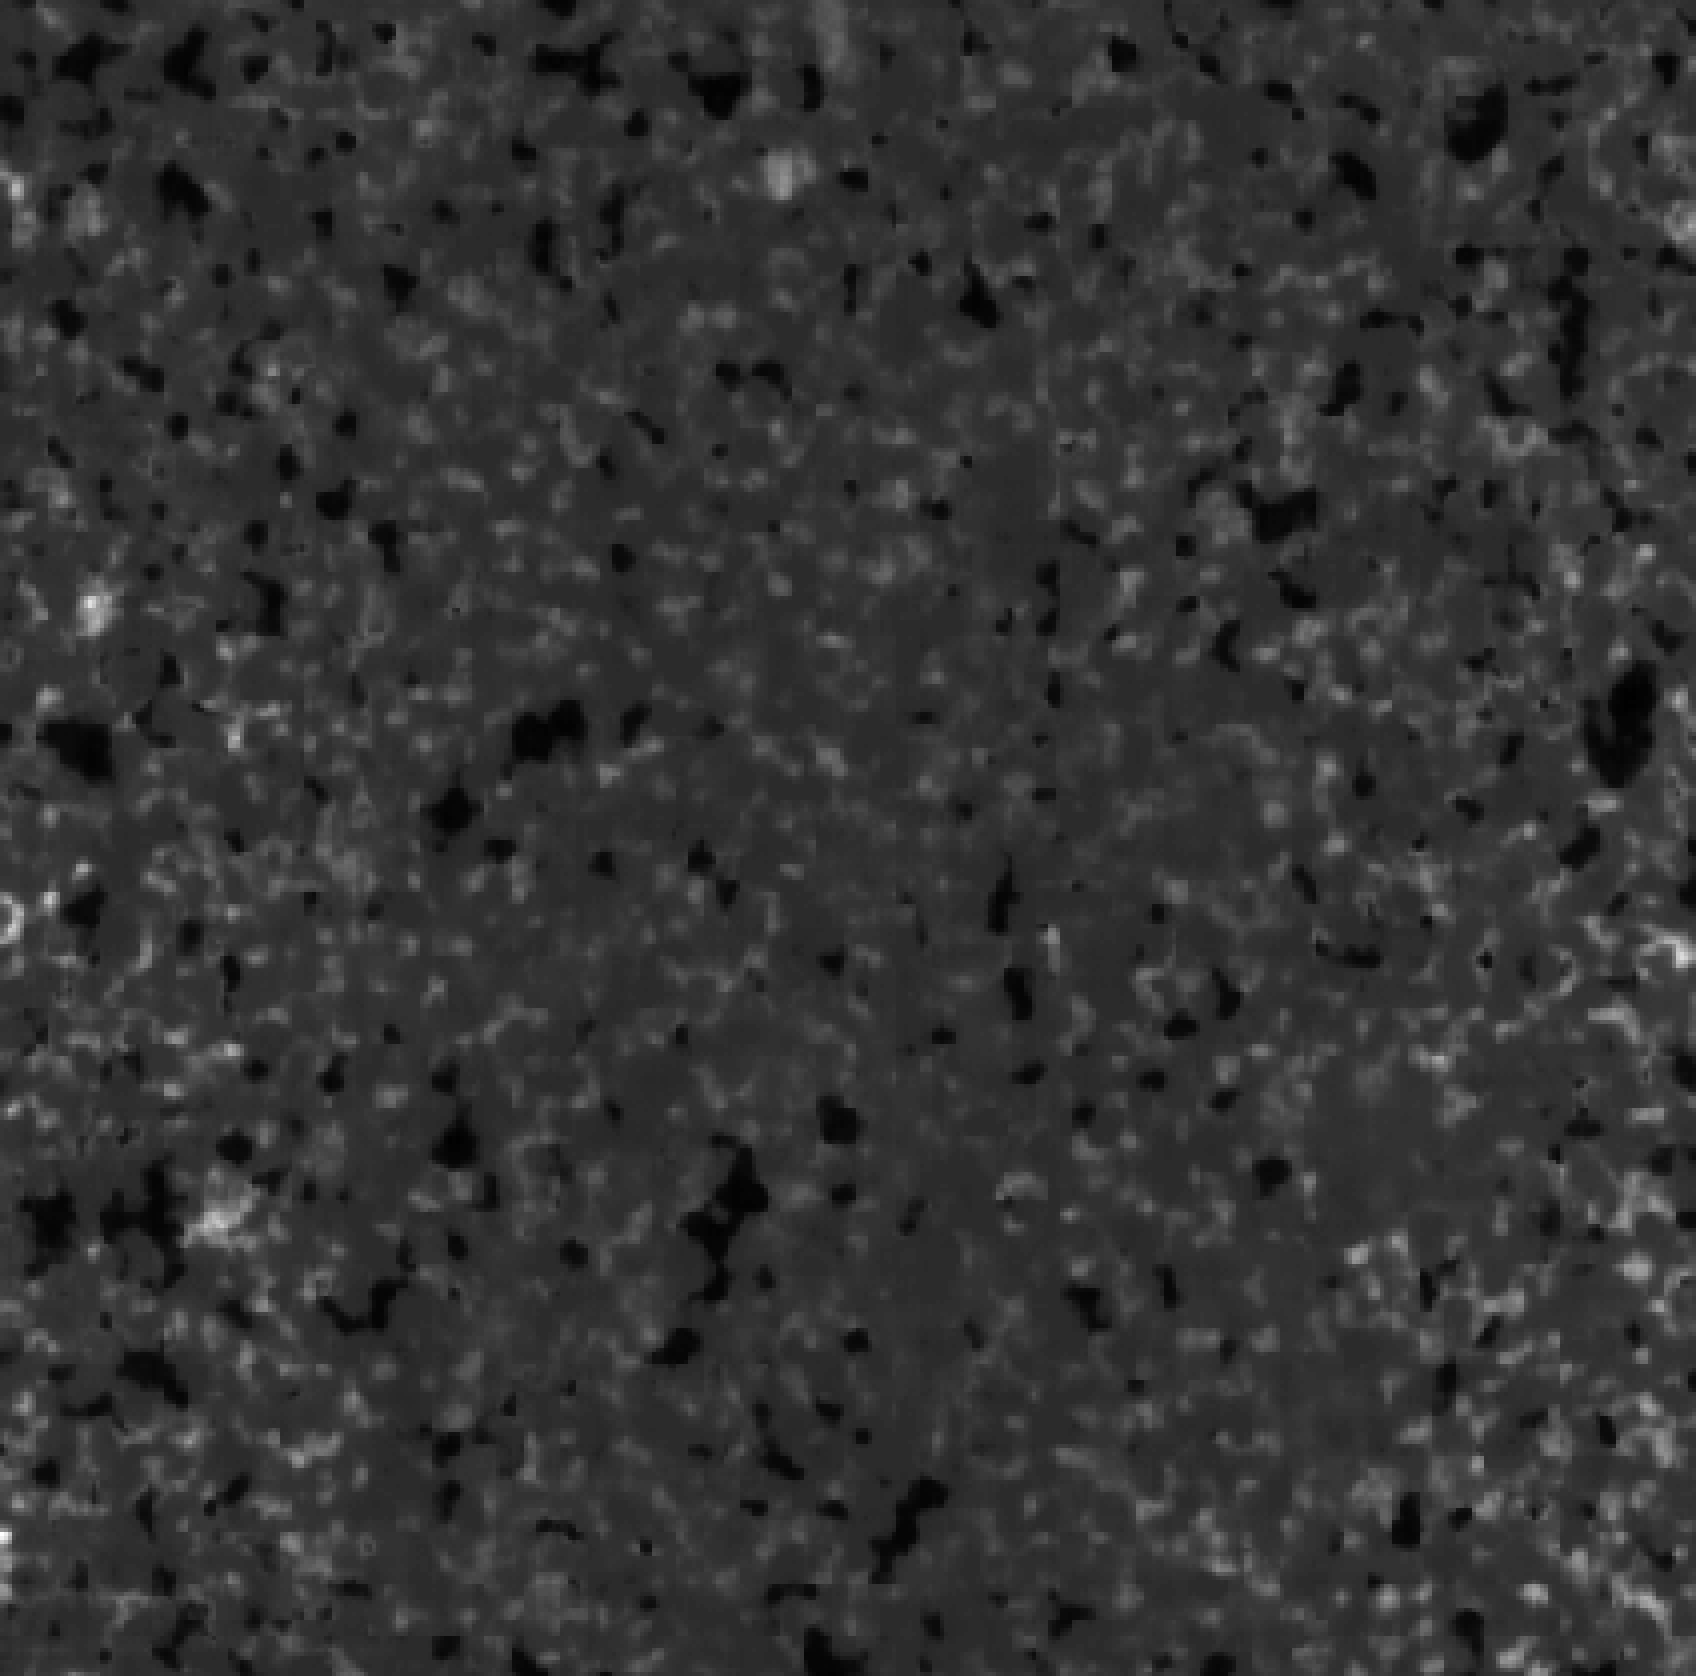
\includegraphics[width=\textwidth]{highcontrast_nect_12h.png}
        \caption{\NeCT{} at 12\,h}
    \end{subfigure}
    \hspace{0.2cm}
    \begin{subfigure}[b]{0.45\textwidth}
        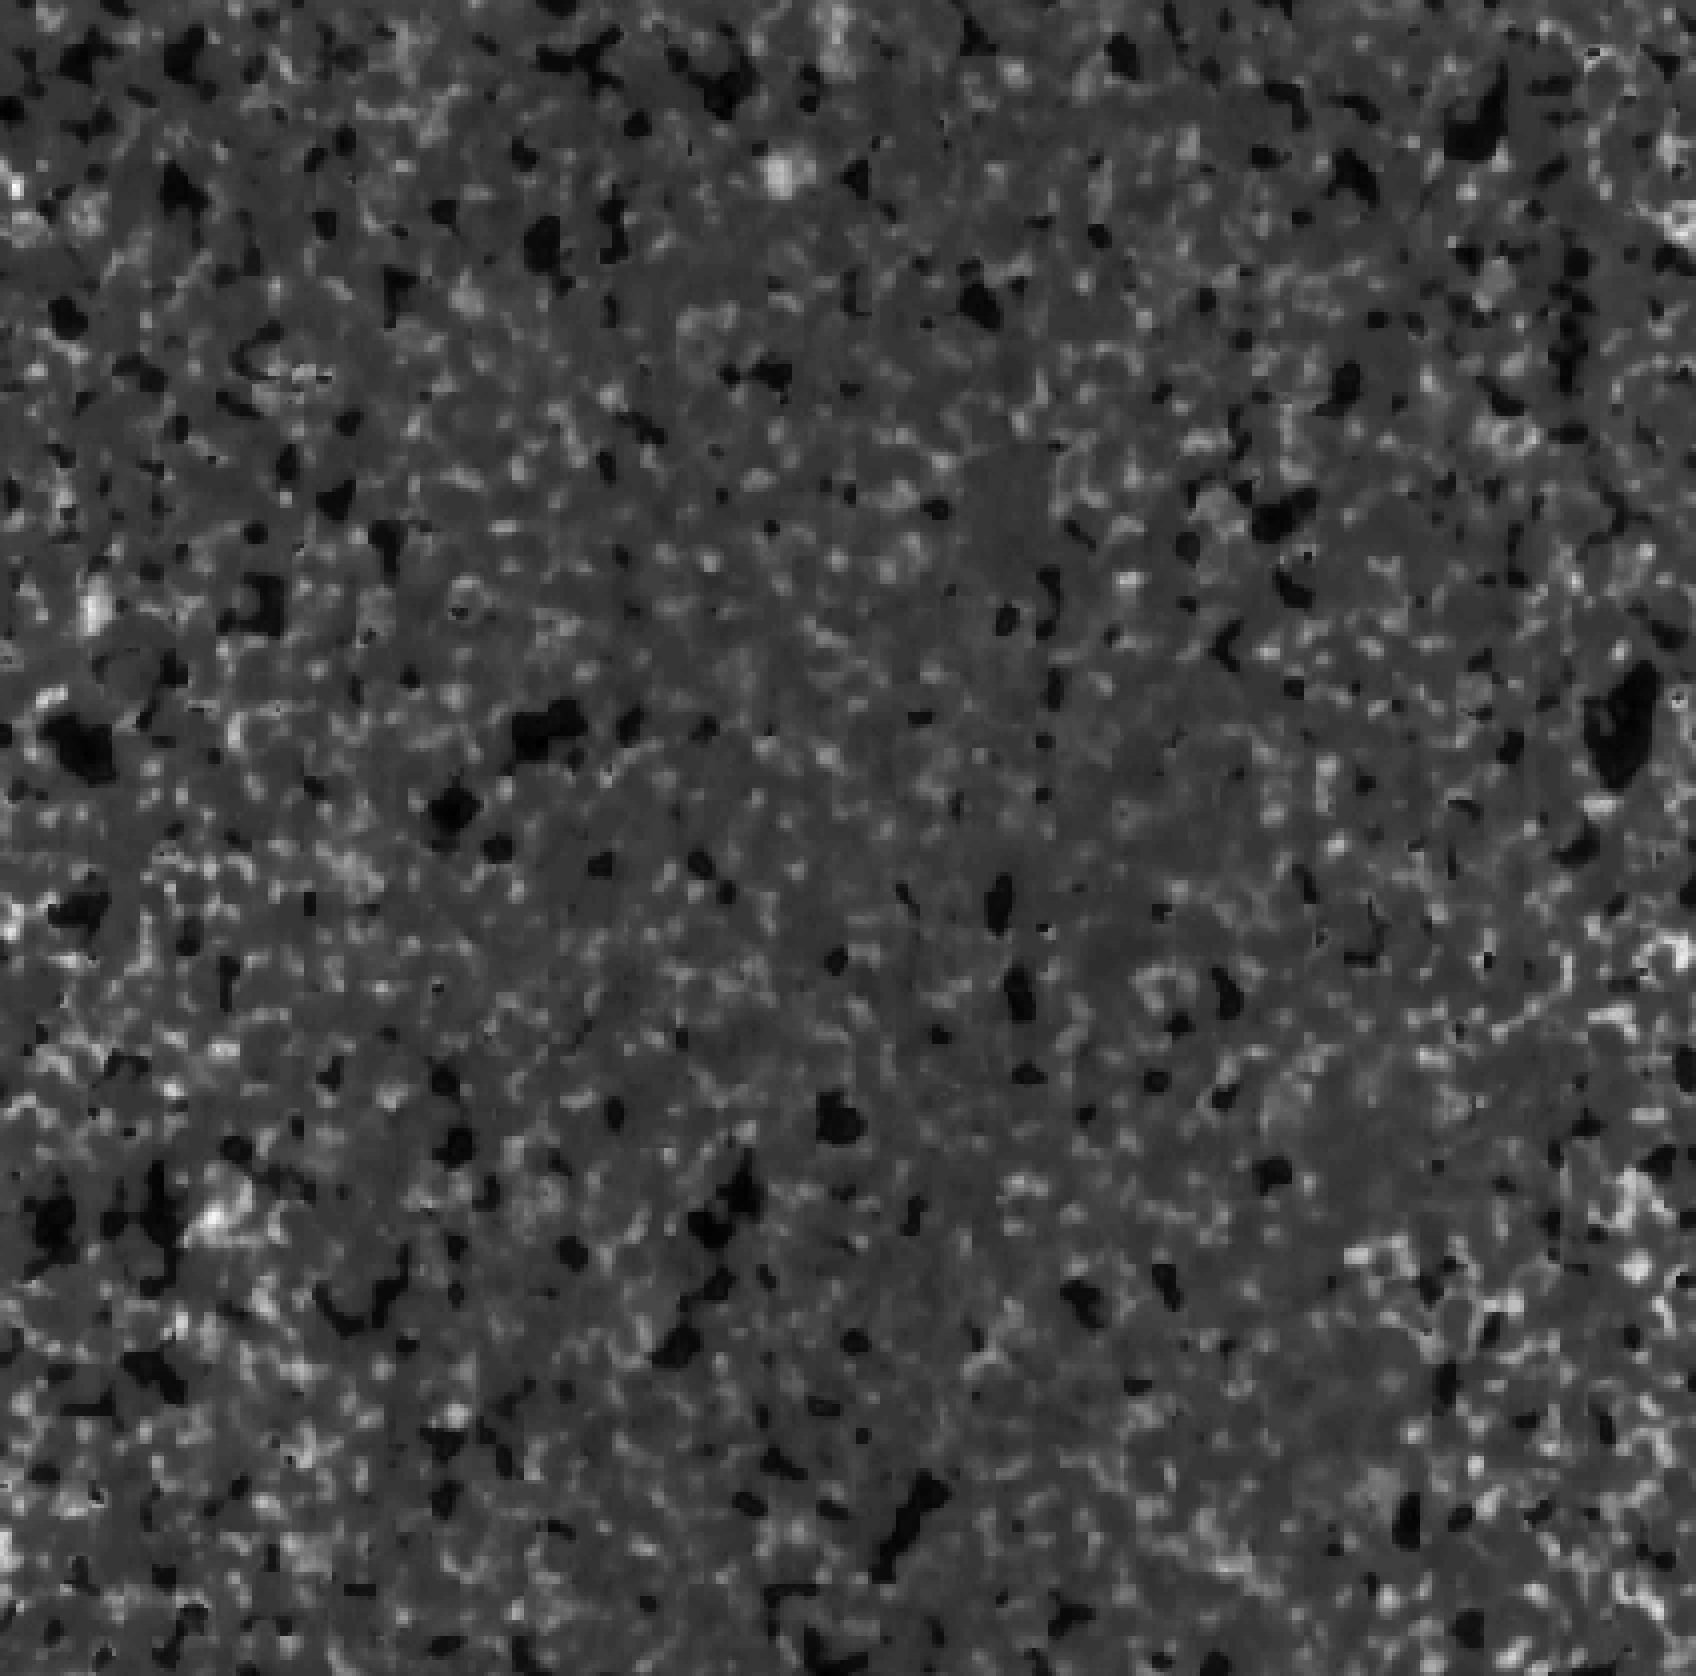
\includegraphics[width=\textwidth]{highcontrast_mixedcubes_12h.png}
        \caption{\MixedCubes{} at 12\,h}
    \end{subfigure}
    \end{adjustwidth}
    \caption{High-contrast reconstruction slices comparing ground truth, the \NeCT{} baseline, and \MixedCubes{} at an equalised 12-hour training budget.}
    \label{fig:mixedcubes_quality}
\end{figure}

Figure~\ref{fig:mixedcubes_quality} shows a high-contrast reconstruction slice at the final timestep of the scan, the most temporally demanding point where fluid has advanced the furthest and spatial gradients are sharpest. Even at this challenging instant, \MixedCubes{} at 12 hours already outperforms the QuadCubes baseline at the same wall-clock budget.

\MixedCubes{} extends CombinedCubes by replacing the three 2D hash-grid temporal encoders with fully dense 2D grids. For 2D encoders the collision-free table size is approximately 4\,MB per level at $1024 \times 1024$ resolution with $F = 4$, which is entirely practical. A dense grid stores one feature vector per grid vertex at every level using the TCNN \texttt{Dense} grid type, with no hash function involved. The grid resolution at level $\ell$ is $R_\text{base} \cdot s^{\ell-1}$ for base resolution $R_\text{base}$ and scale factor $s$. Gradient updates flow directly to the responsible feature vector, completely eliminating hash bucket collisions and the associated gradient interference.

The CombinedCubes temporal encoders are already collision-free at $\log_2 T = 20$, so \MixedCubes{} does not reduce the collision rate further in the strict sense. The benefit of the dense grid is qualitative. The correspondence between spatial coordinates and stored feature vectors is now exact and guaranteed by construction rather than probabilistic. In principle this allows the encoder to represent fine temporal detail with maximal fidelity and without any risk of interference, at the cost of a fixed and larger memory footprint than the hashed variant (the dense grid cannot be downsized by reducing a single parameter the way $\log_2 T$ can).

The dense temporal encoders in the baseline \MixedCubes{} configuration use a base resolution of $R_\text{base} = 16$, a per-level scale factor of $s = 1.5$, and $F = 4$ features per level. The resolution at level $\ell$ is $N_\ell = \lfloor 16 \times 1.5^{\ell-1} \rfloor$, reaching approximately $615 \times 615$ at level 10. All grid vertices are stored explicitly, giving approximately 680\,000 entries per encoder. At float16 precision this is approximately 5.4\,MB per encoder and 16\,MB for the three temporal encoders combined. By contrast, three hashed 2D encoders at $\log_2 T = 20$ with $L = 16$ and $F = 4$ require approximately 260\,MB in total, since each of the nine finest levels stores up to $T = 2^{20}$ feature vectors at 4 features and 2 bytes each. The dense grid is therefore more than an order of magnitude smaller than the hashed alternative at comparable resolution, while guaranteeing an exact coordinate-to-feature mapping. The number of levels and the per-level scale factor are the primary capacity parameters for the temporal encoders and were varied across the \MixedCubes{} configurations shown in the figures below.

\begin{figure}[htbp]
    \begin{adjustwidth}{-2.5cm}{-2.5cm}
    \centering
    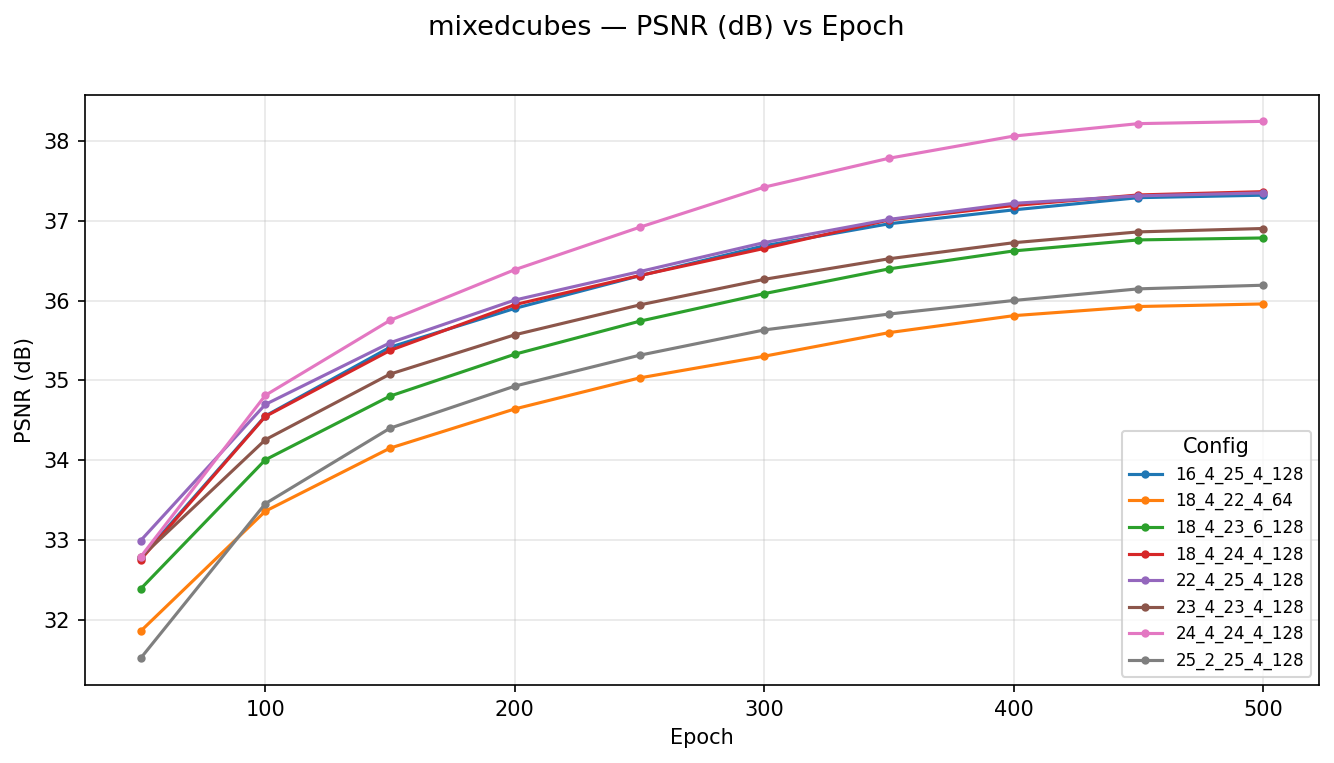
\includegraphics[width=1.1\textwidth]{psnr_arc/mixedcubes_epoch_psnr.png}
    \end{adjustwidth}
    \caption{PSNR vs.\ epoch for the eight representative \MixedCubes{} configurations shown here. The best-performing configuration (\texttt{24\_4\_24\_4\_128}, 22.1\,GB) reaches 38.25\,dB PSNR and SSIM 0.940 at epoch~500, 1.78\,dB above the QuadCubes baseline. The lightweight \texttt{18\_4\_22\_4\_64} (5.1\,GB) reaches 35.96\,dB, nearly matching the baseline at 11\% of its VRAM. Configurations with $F=2$ (the \texttt{25\_2\_} family) underperform relative to $F=4$ equivalents at comparable VRAM. These eight configurations were selected from a larger experimental set to best illustrate performance across the memory, speed, and quality trade-off space.}
    \label{fig:mixedcubes_epoch}
\end{figure}

\begin{figure}[htbp]
    \begin{adjustwidth}{-2.5cm}{-2.5cm}
    \centering
    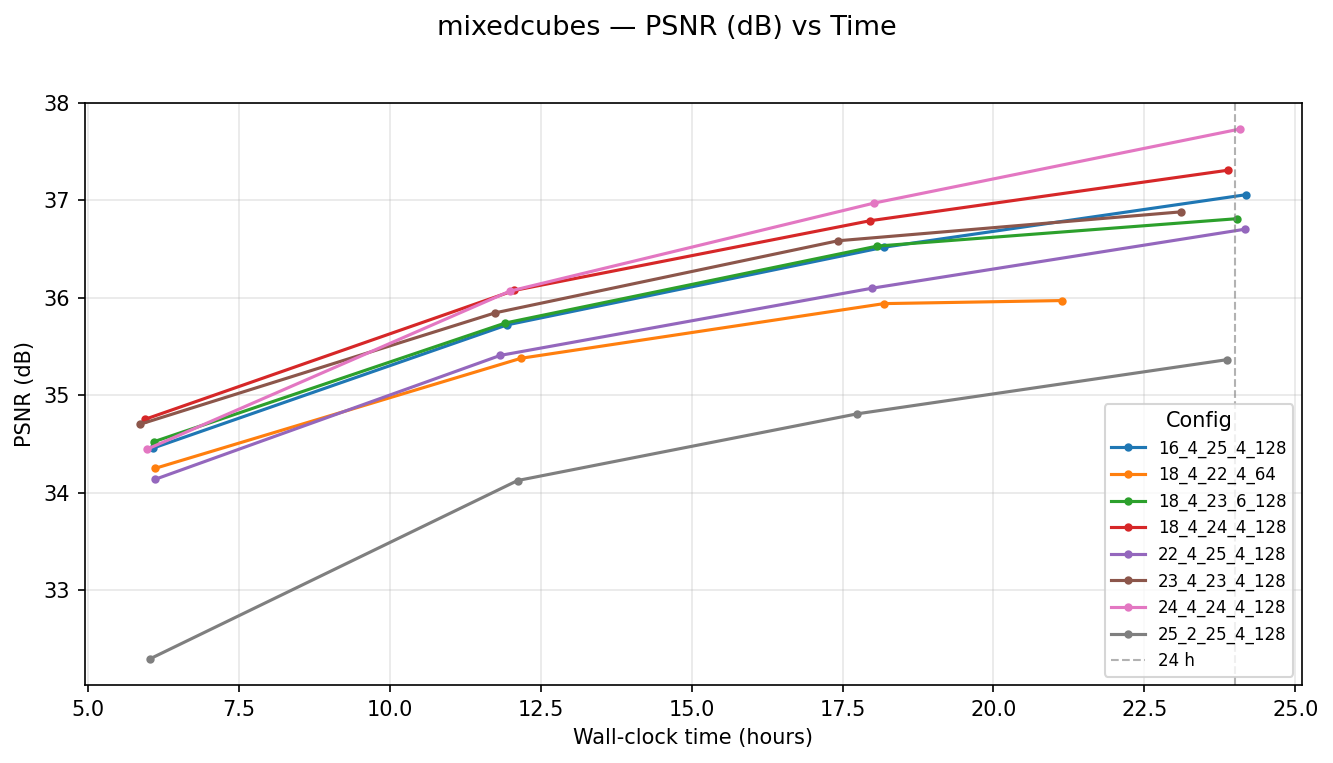
\includegraphics[width=1.1\textwidth]{psnr_arc/mixedcubes_time_psnr.png}
    \end{adjustwidth}
    \caption{PSNR vs.\ wall-clock time for the eight representative \MixedCubes{} configurations. At 24\,h the best configuration (\texttt{24\_4\_24\_4\_128}, 22.1\,GB) achieves 37.73\,dB PSNR, SSIM 0.936, and MAE 2.0 ($+1.84$\,dB over the baseline). The lightweight \texttt{18\_4\_22\_4\_64} (5.1\,GB) reaches 35.97\,dB within 0.08\,dB of the baseline at roughly one ninth of the VRAM. The $F=2$ configuration \texttt{25\_2\_25\_4\_128} (25.5\,GB) reaches only 35.37\,dB at 24\,h, 0.52\,dB below the baseline despite its large hashmap, confirming that $F=2$ is counterproductive in the split-encoder context. These configurations were selected to best represent the experimental landscape.}
    \label{fig:mixedcubes_time}
\end{figure}

The eight \MixedCubes{} configurations shown here were selected from a larger experimental set to best illustrate the range of performance across different memory, training time, and quality trade-offs.

Figures~\ref{fig:mixedcubes_epoch} and \ref{fig:mixedcubes_time} show that \MixedCubes{} consistently outperforms the QuadCubes baseline. At the 24-hour mark the best configuration (\texttt{24\_4\_24\_4\_128}, 22.1\,GB) achieves PSNR 37.73\,dB, SSIM 0.936, and MAE 2.0, a gain of $+1.84$\,dB in PSNR, $+0.024$ in SSIM, and $-0.5$ in MAE over the baseline (35.89\,dB, SSIM 0.912, MAE 2.5) at half the VRAM. Notably, \texttt{18\_4\_22\_4\_64} (5.1\,GB) reaches 35.97\,dB at 21\,h, within 0.08\,dB of the baseline while using only 11\% of the baseline's 44.8\,GB. At epoch~500, \texttt{24\_4\_24\_4\_128} reaches 38.25\,dB with SSIM 0.940 and MAE 1.9. The \texttt{23\_4\_23\_4\_128} configuration (13.1\,GB) achieves 36.88\,dB PSNR at 23\,h, approximately $+0.99$\,dB above the baseline at less than one third of its VRAM.

A consistent finding across \MixedCubes{} configurations is that $F=2$ (halved feature dimension) is counterproductive. The \texttt{20\_2\_24\_4\_128} configuration (10.8\,GB, $F=2$ on temporal encoders) achieves 36.57\,dB at 24\,h, which is positive but lower than several smaller $F=4$ configurations. More starkly, \texttt{25\_2\_25\_4\_128} (25.5\,GB), which uses a very large temporal hashmap but only $F=2$ features, reaches only 35.37\,dB at 24\,h, 0.52\,dB below the QuadCubes baseline despite consuming more than half the baseline VRAM. The large hashmap does not compensate for the reduced feature capacity. In the split-encoder context, where the temporal encoders are already small and operating near the collision-free regime, reducing $F$ removes representational capacity that the model actually needs.

Decoder depth has a modest and configuration-dependent effect. The best-performing \MixedCubes{} configurations use 4 hidden layers, and increasing to 6 does not consistently improve results.

\subsection{Architecture and Problem Structure}
\label{subsec:asymmetry_synthesis}

The non-uniform sizing experiments confirm the spatial-temporal asymmetry hypothesis. Redirecting hashmap capacity from temporal to spatial encoders improves quality on all three metrics at substantially lower VRAM. Temporal-heavy configurations, by contrast, perform well below the baseline despite comparable memory budgets. Increasing temporal encoder capacity within the QuadCubes architecture returns far less quality per byte than the same increase applied to the spatial encoder.

CombinedCubes takes this finding to its structural conclusion. By replacing the three 3D temporal encoders with collision-free 2D temporal encoders, it reduces memory substantially and achieves better reconstruction quality across all metrics at lower VRAM than the baseline. The best CombinedCubes configuration at 24\,h ($+1.39$\,dB, 18.3\,GB) outperforms the baseline at less than half the VRAM. The impact of switching only the temporal encoders is clearest in the \MixedCubes{} \ texttt{23\_4\_23\_4\_128} configuration, which uses an identical spatial encoder to the QuadCubes baseline but replaces the three temporal 3D hash encoders with dense 2D grids. Total VRAM drops from 44.8\,GB to 13.1\,GB. The QuadCubes baseline reaches 36.47\,dB at epoch~500, which takes approximately 43 hours. \MixedCubes{} \texttt{23\_4\_23\_4\_128} surpasses that quality level after only 21 hours. \MixedCubes{} takes this a step further by replacing the hashed 2D temporal encoders with fully dense grids, guaranteeing an exact coordinate-to-feature correspondence and yielding the best 24-hour result across all architectures ($+1.84$\,dB, 22.1\,GB). Decoder depth has a modest and configuration-dependent effect in both architectures. The best results use 4 hidden layers, though some 6-layer configurations achieve higher quality at epoch convergence. Four layers are sufficient for the strongest 24-hour results, and the architectural separation does not impose a fundamental additional burden on the decoder.

The third design principle follows from this. The encoder architecture should reflect the asymmetry between the spatial and temporal components of the problem. The spatial encoder benefits from high-dimensional encoding with adequate hashmap size, while the temporal encoders benefit from low-dimensional, collision-free encoding suited to the lower-frequency temporal signal. Within this split-encoder context, the feature dimension $F$ should be kept at 4 for both encoder types. Halving $F$ on the temporal encoders eliminates capacity that is genuinely needed rather than redundant, as the $F = 2$ results in both CombinedCubes and \MixedCubes{} consistently demonstrate.

% ═════════════════════════════════════════════════════════════════════════════
\chapter{Encoder Comparison}
\label{chap:encoder_comparison}
% ═════════════════════════════════════════════════════════════════════════════

Chapter~\ref{chap:encoder_design} established three design principles for the NeCT encoder, each derived from the interplay between a capacity parameter and its corresponding architectural extreme. The hashmap size governs precision per parameter through collision load, and SingleCube demonstrates the catastrophic case. The number of levels governs precision per training hour through frequency coverage and per-step cost, and HexCubes demonstrates the failure mode of sacrificing coordinate coupling to achieve collision-free low-dimensional encoders. The spatial-temporal asymmetry means the optimal encoder treats the spatial and temporal components differently, as confirmed by the non-uniform sizing experiments, the CombinedCubes results, and the \MixedCubes{} results.

The practical question that follows is which configuration should be recommended for practical 4D-CT reconstruction. Four configurations spanning the key design choices explored in Chapter~\ref{chap:encoder_design} are compared against each other and against the original NeCT baseline on a common footing.

\section{Candidate Configurations}
\label{sec:comp_candidates}

Three configurations are compared.

\begin{itemize}
    \item \textbf{NeCT baseline.} The original QuadCubes configuration from \citet{friis2025nect} with uniform encoders at $L = 23$, $\log_2 T = 23$, $F = 4$. This is the reference point, representing the largest configuration the original paper considered.
    \item \textbf{Spatial-heavy QuadCubes.} Configuration \texttt{24\_4\_24\_4\_128} from \cref{subsec:nonuniform_sizing}, enlarging the spatial \texttt{xyz} encoder relative to the three temporal encoders. Best at 24\,h: 37.53\,dB PSNR, SSIM 0.934, MAE 2.1, at 24.1\,GB VRAM.
    \item \textbf{CombinedCubes (best).} Configuration \texttt{18\_4\_24\_4\_128} from \cref{subsec:combinedcubes}: 3D spatial hash encoder with three collision-free 2D hash temporal encoders (18.3\,GB). Best at 24\,h: 37.28\,dB PSNR, SSIM 0.926, MAE 2.1.
    \item \textbf{\MixedCubes{} (best).} Configuration \texttt{24\_4\_24\_4\_128} from \cref{subsec:mixedcubes}, using a 3D spatial hash encoder and three fully dense 2D temporal encoders at 22.1\,GB VRAM. This is the highest-scoring architecture at the 24-hour mark (37.73\,dB PSNR, SSIM 0.936, MAE 2.0) and at epoch~500 (38.25\,dB PSNR, SSIM 0.940, MAE 1.9).
\end{itemize}

\section{Unified Comparison}
\label{sec:comp_results}

Table~\ref{tab:full_comparison} summarises reconstruction quality, peak GPU memory, and training time for all three candidates at equalised training budgets of 14 and 24 hours.

\begin{table}[h]
    \begin{adjustwidth}{-2cm}{0cm}
    \centering
    \caption{Comparison of the NeCT baseline against the best spatial-heavy QuadCubes, CombinedCubes, and \MixedCubes{} configurations at 24\,h wall-clock time and at epoch~500. All results on the Bentheimer sandstone dataset.}
    \label{tab:full_comparison}
    \begin{tabular}{llllll}
        \toprule
        Configuration & PSNR (dB) & SSIM & MAE & VRAM (GB) & Time (h) \\
        \midrule
        NeCT baseline (QuadCubes)                   & 35.89 & 0.912 & 2.5 & 44.8 & 24 \\
        Spatial-heavy QuadCubes \texttt{24\_4\_24\_4\_128}  & 37.53 & 0.934 & 2.1 & 24.1 & 24 \\
        CombinedCubes \texttt{18\_4\_24\_4\_128}          & 37.28 & 0.926 & 2.1 & 18.3 & 24 \\
        \MixedCubes{} \texttt{24\_4\_24\_4\_128}          & 37.73 & 0.936 & 2.0 & 22.1 & 24 \\
        \midrule
        NeCT baseline (QuadCubes)                   & 36.47 & 0.921 & 2.4 & 44.8 & ep.\,500 \\
        Spatial-heavy QuadCubes \texttt{24\_4\_24\_4\_128}  & 37.86 & 0.934 & 2.1 & 24.1 & ep.\,500 \\
        CombinedCubes \texttt{24\_4\_24\_6\_128}          & 38.88 & 0.945 & 1.8 & 24.3 & ep.\,500 \\
        \MixedCubes{} \texttt{24\_4\_24\_4\_128}          & 38.25 & 0.940 & 1.9 & 22.1 & ep.\,500 \\
        \bottomrule
    \end{tabular}
    \end{adjustwidth}
\end{table}

\begin{figure}[htbp]
    \begin{adjustwidth}{-2.5cm}{-2.5cm}
    \centering
    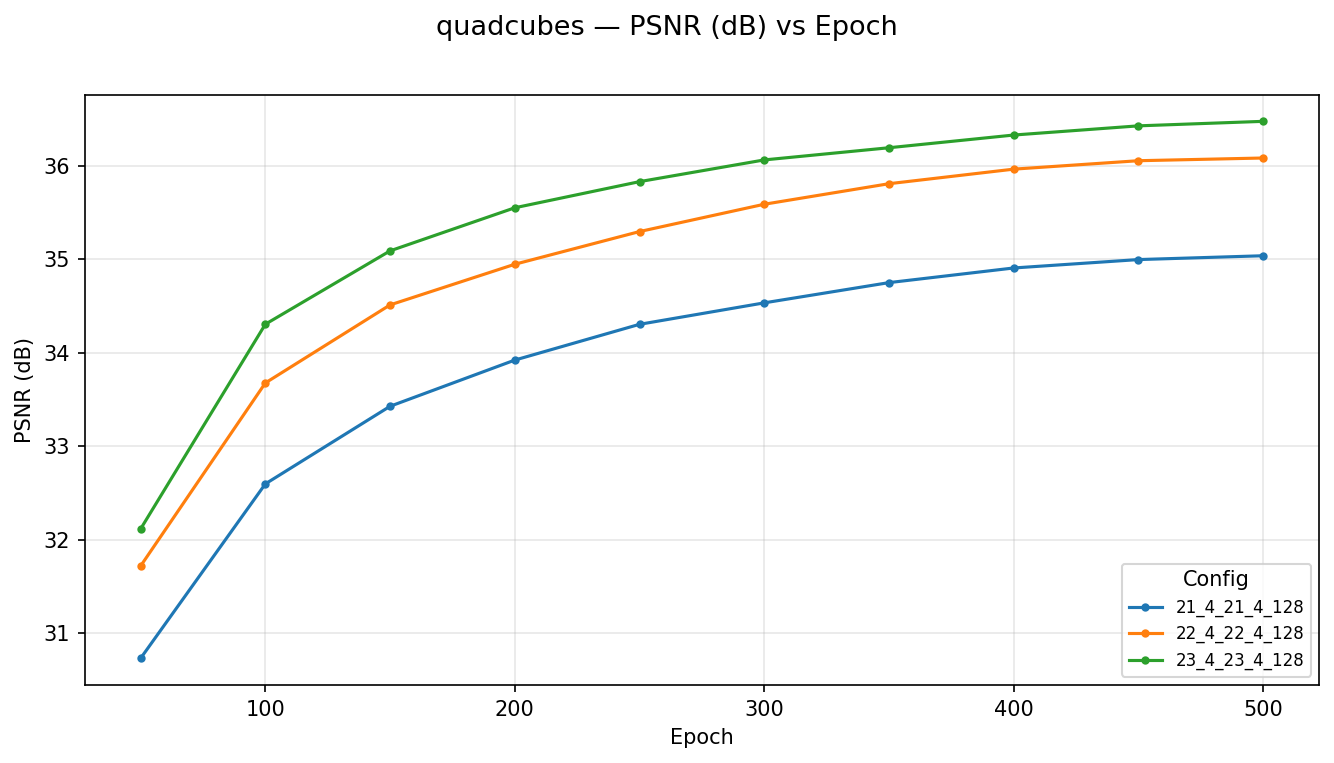
\includegraphics[width=1.1\textwidth]{psnr_arc/quadcubes_epoch_psnr.png}
    \end{adjustwidth}
    \caption{PSNR vs.\ epoch for QuadCubes configurations. The baseline (\texttt{23\_4\_23\_4\_128}, 44.8\,GB) reaches 36.47\,dB at epoch~500. The mid-size config (\texttt{22\_4\_22\_4\_128}, 23.1\,GB) reaches 36.08\,dB, and the smallest (\texttt{21\_4\_21\_4\_128}, 11.9\,GB) reaches 35.04\,dB.}
    \label{fig:quadcubes_all_epoch}
\end{figure}

\begin{figure}[htbp]
    \begin{adjustwidth}{-2.5cm}{-2.5cm}
    \centering
    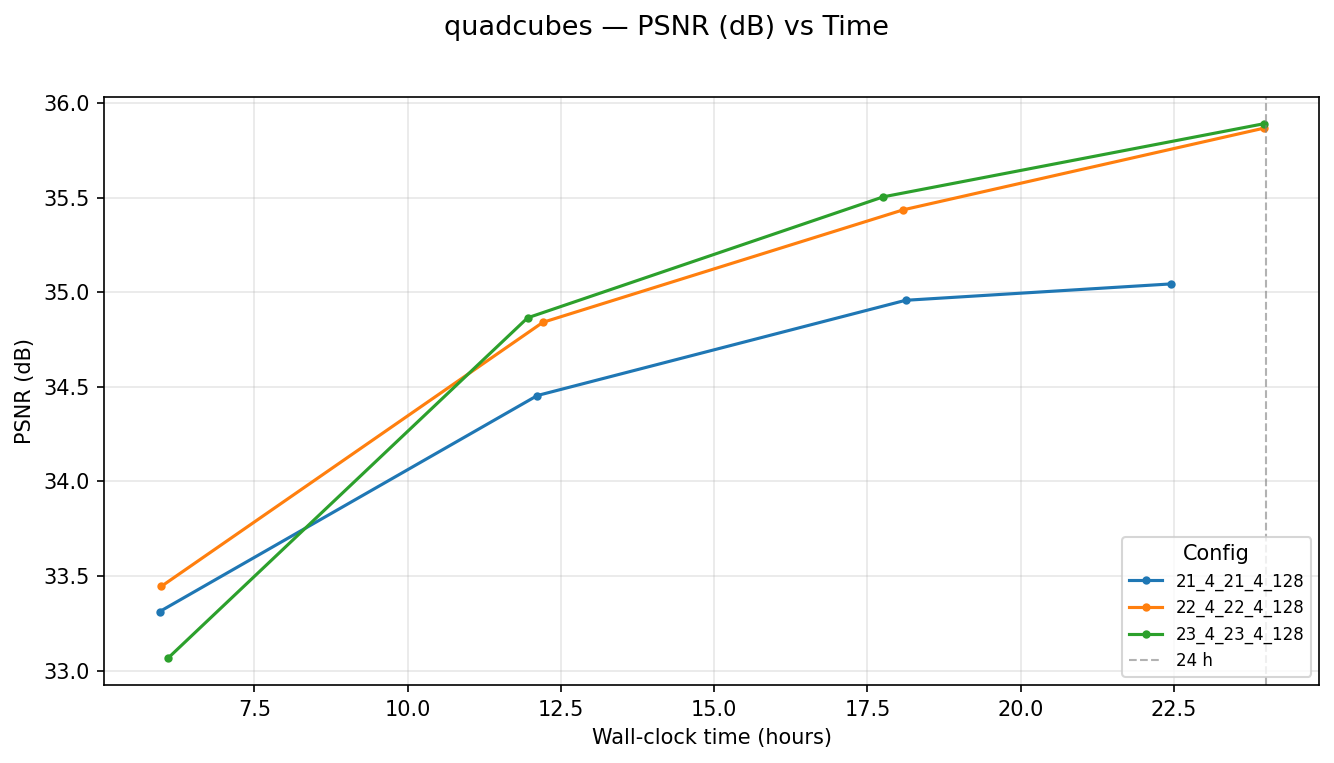
\includegraphics[width=1.1\textwidth]{psnr_arc/quadcubes_time_psnr.png}
    \end{adjustwidth}
    \caption{PSNR vs.\ wall-clock time for QuadCubes configurations. At 24\,h the baseline achieves 35.89\,dB (SSIM 0.912, MAE 2.5, 44.8\,GB); the mid-size config achieves 35.87\,dB (SSIM 0.909, MAE 2.6, 23.1\,GB), essentially identical quality at half the VRAM.}
    \label{fig:quadcubes_all_time}
\end{figure}

The QuadCubes results establish an important reference point. In the epoch plot, the three configurations separate cleanly by hashmap size, with the baseline (44.8\,GB) reaching 36.47\,dB, the mid-size configuration (23.1\,GB) reaching 36.08\,dB, and the smallest (11.9\,GB) reaching 35.04\,dB. The quality gap between baseline and mid-size is only 0.39\,dB despite a near-doubling of VRAM. In the wall-clock time plot this gap narrows further. The mid-size configuration reaches 35.87\,dB at 24\,h versus the baseline's 35.89\,dB, essentially indistinguishable quality at half the memory. This confirms the finding from the hashmap sweep that the baseline is operating past the point of diminishing returns, as the additional parameters do not return proportional quality gains. Within the QuadCubes family, there is therefore no reason to use the full-size baseline configuration unless memory is unconstrained and convergence time is the only concern.

\begin{figure}[htbp]
    \begin{adjustwidth}{-2.5cm}{-2.5cm}
    \centering
    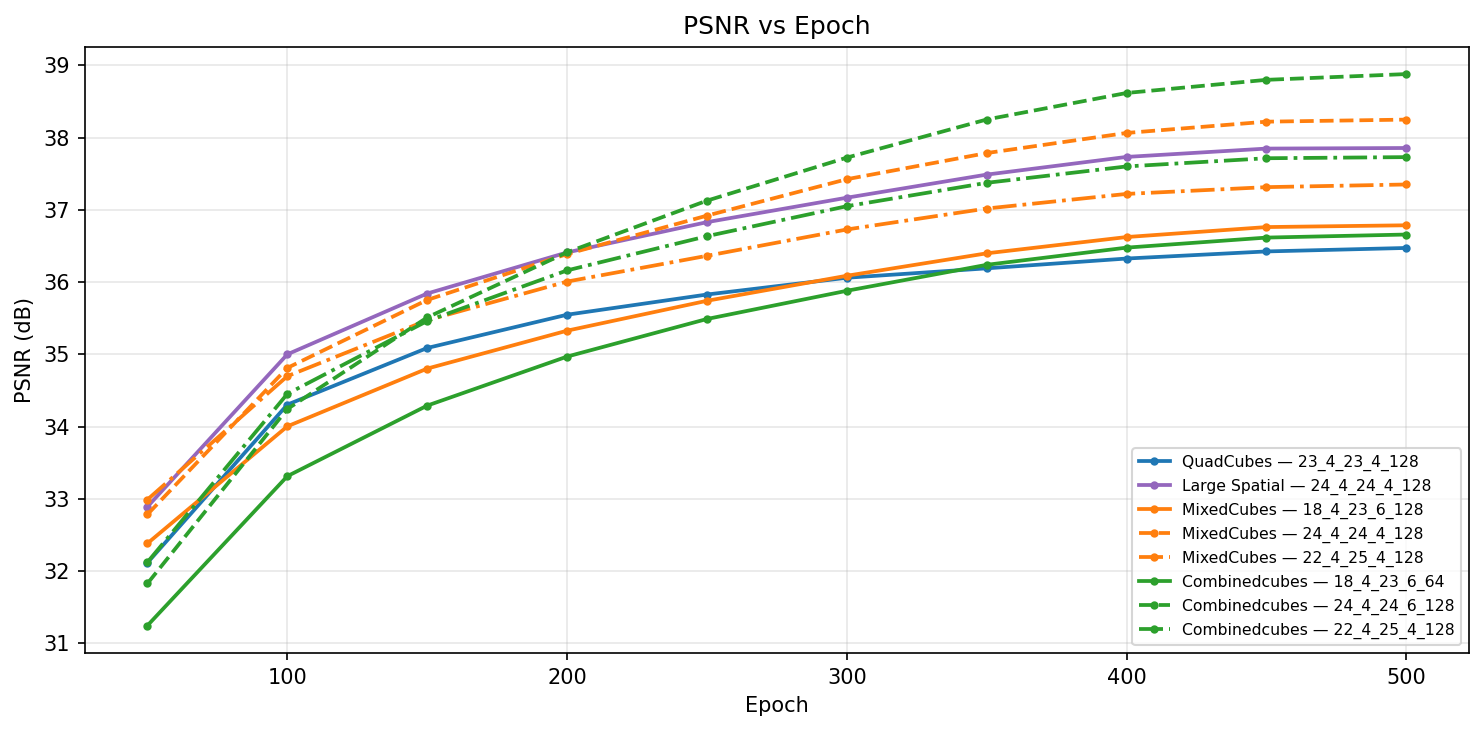
\includegraphics[width=1.1\textwidth]{top2/all_psnr_epoch.png}
    \end{adjustwidth}
    \caption{PSNR vs.\ epoch for representative configurations of each architecture: QuadCubes baseline (\texttt{23\_4\_23\_4\_128}), spatial-heavy QuadCubes (\texttt{24\_4\_24\_4\_128}), three \MixedCubes{} variants (\texttt{18\_4\_23\_6\_128}, \texttt{24\_4\_24\_4\_128}, \texttt{22\_4\_25\_4\_128}), and three CombinedCubes variants (\texttt{18\_4\_23\_6\_64}, \texttt{24\_4\_24\_6\_128}, \texttt{22\_4\_25\_4\_128}).}
    \label{fig:combined_epoch}
\end{figure}

\begin{figure}[htbp]
    \begin{adjustwidth}{-2.5cm}{-2.5cm}
    \centering
    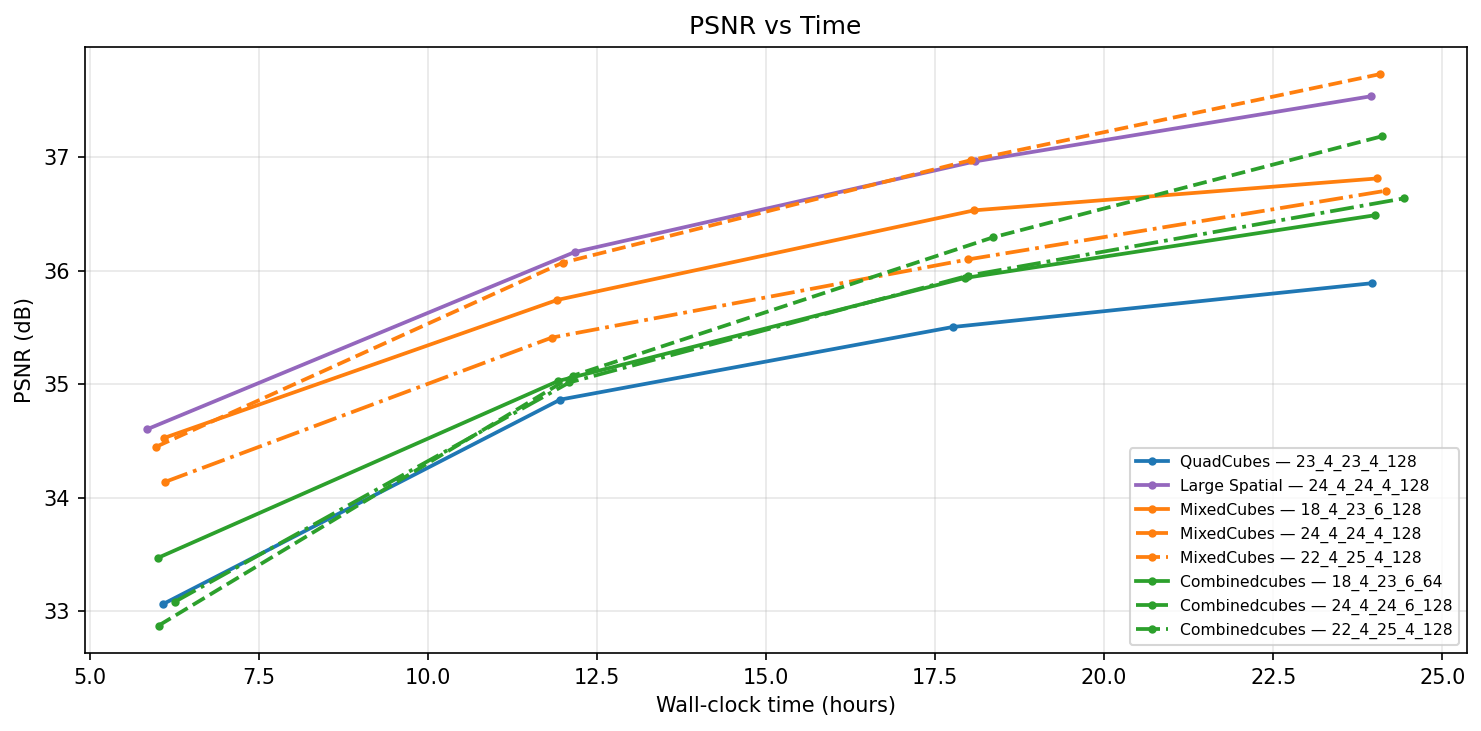
\includegraphics[width=1.1\textwidth]{top2/all_psnr_time.png}
    \end{adjustwidth}
    \caption{PSNR vs.\ wall-clock time for the same configurations as Figure~\ref{fig:combined_epoch}. The dashed vertical line marks the 24\,h comparison point.}
    \label{fig:combined_time}
\end{figure}

The epoch plot (Figure~\ref{fig:combined_epoch}) reveals a clear separation between architectures that persists across all training stages. At epoch~500 CombinedCubes \texttt{24\_4\_24\_6\_128} leads at 38.88\,dB, followed closely by \MixedCubes{} \texttt{24\_4\_24\_4\_128} at 38.25\,dB and spatial-heavy QuadCubes at 37.86\,dB, with the uniform baseline at 36.47\,dB. The fact that CombinedCubes reaches the highest asymptotic quality suggests it has a slightly higher quality ceiling, likely because its larger decoder and hash-grid temporal encoders provide additional representational headroom when given sufficient training time.

The wall-clock time plot (Figure~\ref{fig:combined_time}) tells a meaningfully different story and is the more practically relevant comparison. \MixedCubes{} outperforms CombinedCubes substantially in the first twelve hours of training. Because \MixedCubes{} temporal encoders are dense grids rather than hashed tables, each training step is faster and more epochs are completed within any fixed time budget. The quality advantage that CombinedCubes eventually accumulates in epoch space is therefore not accessible within typical reconstruction turnaround windows. For any workflow constrained to 24 hours or fewer, \MixedCubes{} is the superior choice. The two architectures converge in epoch-quality performance at high epoch counts but diverge sharply in time-quality performance — the dense temporal grids of \MixedCubes{} make it both faster per step and more memory-efficient, which compounds into a large practical advantage.

\begin{figure}[htbp]
    \begin{adjustwidth}{-2.5cm}{-2.5cm}
    \centering
    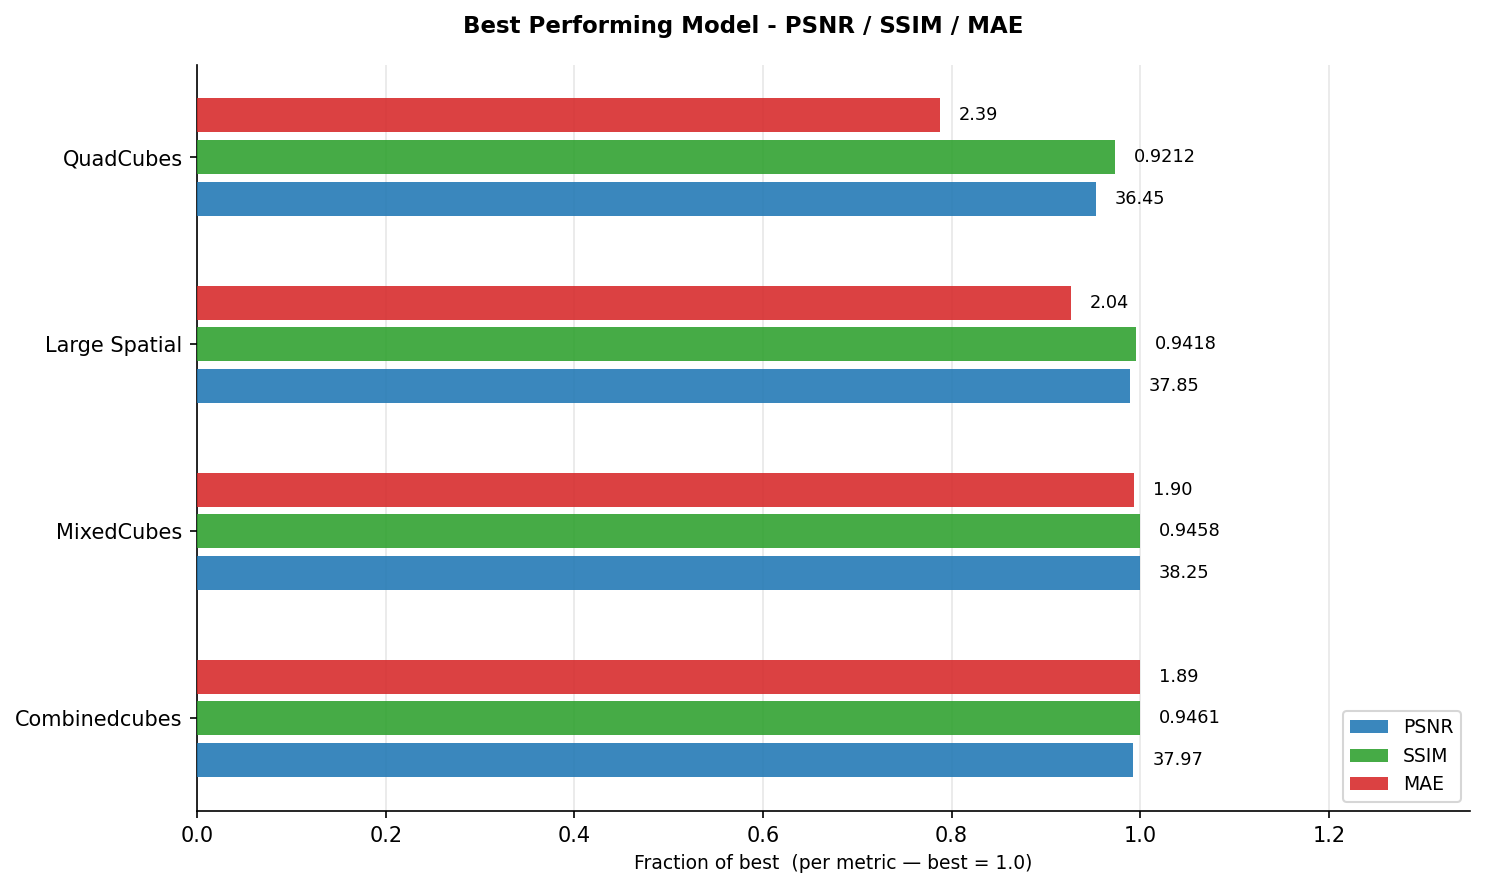
\includegraphics[width=1.1\textwidth]{top2/metrics_bar.png}
    \end{adjustwidth}
    \caption{PSNR, SSIM, and MAE at 24\,h for the best-performing configuration of each architecture: QuadCubes baseline, spatial-heavy QuadCubes (\texttt{24\_4\_24\_4\_128}), CombinedCubes (\texttt{18\_4\_24\_4\_128}), and \MixedCubes{} (\texttt{24\_4\_24\_4\_128}). Higher bars indicate better PSNR and SSIM; lower bars indicate better MAE.}
    \label{fig:top2_comparison}
\end{figure}

Figure~\ref{fig:top2_comparison} confirms that the rankings observed in PSNR are consistent across all three evaluation metrics. SSIM and MAE produce the same ordering, and the improvements over the baseline are positive on every metric simultaneously. The quality advantage of the split-encoder architectures is therefore not an artefact of PSNR sensitivity to any particular error pattern.

\begin{figure}[htbp]
    \begin{adjustwidth}{-2.5cm}{-2.5cm}
    \centering
    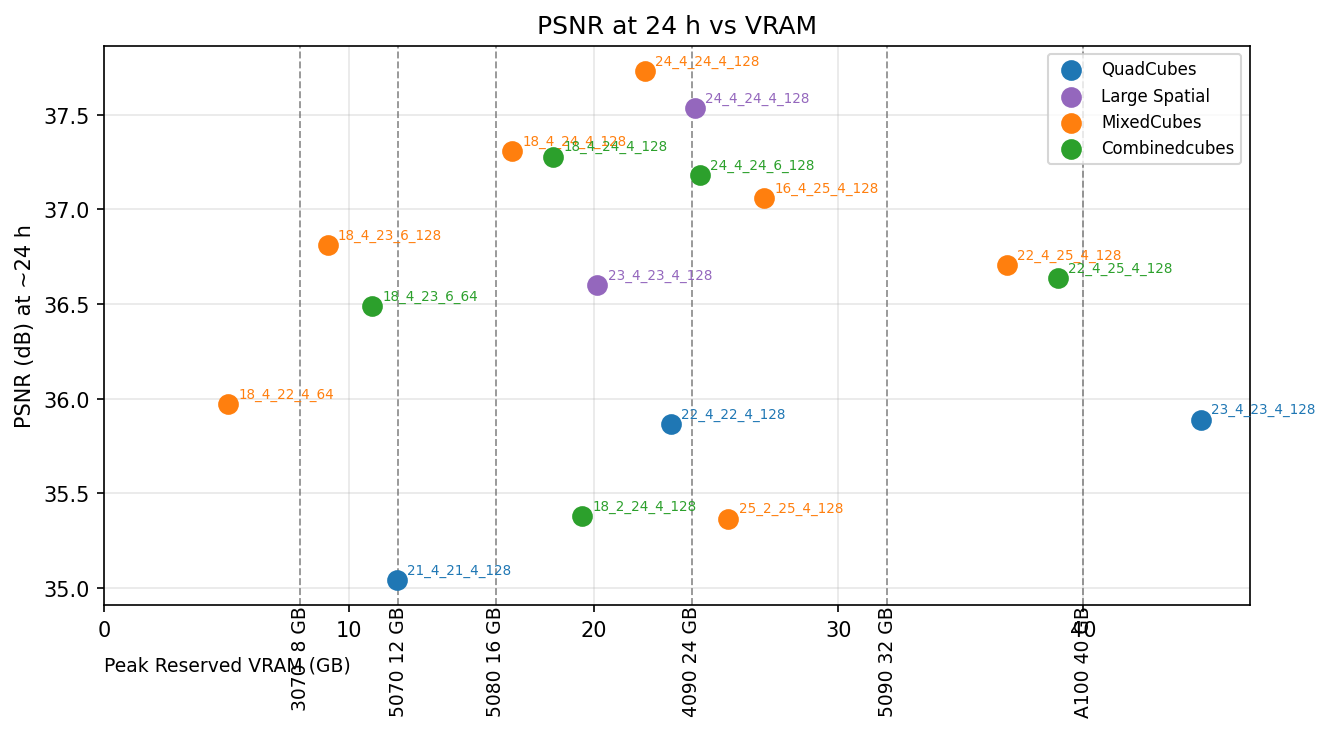
\includegraphics[width=1.1\textwidth]{top2/all_vram2.png}
    \end{adjustwidth}
    \caption{PSNR at 24\,h versus peak training VRAM for all configurations evaluated. Each point is one experimental run; colours distinguish architecture families. Triangular markers identify $F=2$ configurations within the split-encoder families.}
    \label{fig:vram_efficiency}
\end{figure}

Figure~\ref{fig:vram_efficiency} places all configurations on a common quality-versus-memory plane and is the most information-dense result of this chapter. Four patterns warrant detailed discussion.

The $F=2$ configurations (triangular markers) cluster in the lower portion of the plot, below the QuadCubes baseline and in some cases below the smallest QuadCubes variant. This is the most striking failure mode in the experimental set. These configurations have large hashmaps — some exceeding 25\,GB — yet they underperform models that use a fraction of their memory. The explanation lies in the split-encoder structure. In the split-encoder architectures, the temporal encoders are already operating near or at the collision-free regime, there is no forced-collision problem left for additional hash capacity to solve. Halving the feature dimension $F$ removes representational capacity that is genuinely needed for the encoder to express the temporal signal, and this capacity loss cannot be compensated by increasing the hashmap size. The $F=2$ models illustrate that memory budget and model quality are not simply correlated — misallocated capacity actively harms performance.

The \MixedCubes{} configurations form a clear Pareto frontier, with \texttt{18\_4\_22\_4\_64} (5.1\,GB), \texttt{18\_4\_23\_6\_128} (9.1\,GB), \texttt{18\_4\_24\_4\_128} (18.3\,GB -- note this is a CombinedCubes configuration at similar VRAM), and \texttt{24\_4\_24\_4\_128} (22.1\,GB) occupying the upper-left edge of the plot. For every VRAM level from 5\,GB to 22\,GB, a \MixedCubes{} configuration achieves the highest quality of any architecture tested. No QuadCubes or CombinedCubes configuration at a given memory level outperforms the corresponding \MixedCubes{} point.

The \texttt{XX\_4\_25} configurations — those with a large $\log_2 T = 25$ hashmap in either the spatial or temporal encoder — show a consistent performance shortfall relative to their \texttt{XX\_4\_24} equivalents despite consuming more VRAM. This represents a soft ceiling on the benefit of increasing hashmap size for collision reduction. At $\log_2 T = 24$ the per-level collision rate is already low enough that further reduction via a larger table returns negligible quality improvement, while the additional parameters and the longer time required to update them within a 24-hour budget actively reduce the quality achieved per unit time. The result is that \texttt{XX\_4\_25} configurations are dominated by their \texttt{XX\_4\_24} counterparts on the VRAM-quality plane.

Finally, the \texttt{24\_4\_24} configuration, the top performer across spatial-heavy QuadCubes, \MixedCubes{}, and CombinedCubes, forms a visible cluster in the upper-middle region of the plot at approximately 22--24\,GB. This convergence across architectures suggests that $\log_2 T = 24$ with $F = 4$ represents a near-optimal capacity point for the spatial encoder at micro-CT resolutions. It is large enough to achieve low collision rates and near-saturation quality, and small enough to fit within practical VRAM budgets. Within this cluster the \MixedCubes{} implementation achieves marginally higher quality at slightly lower VRAM than the CombinedCubes equivalent, and crucially falls below the 24\,GB threshold that separates consumer and professional-grade GPUs.

\section{Discussion}
\label{sec:comp_discussion}

\subsection{What the Three Configurations Represent}
\label{subsec:comp_disc_interpretation}

The four candidates represent a progression of design decisions rather than arbitrary points on a continuous axis. The NeCT baseline is the upper bound of the original design paradigm, using uniform capacity across all four encoders with no attempt to exploit the spatial-temporal asymmetry. The results show it is neither the most memory-efficient nor the highest quality. Every other candidate here exceeds its reconstruction quality at lower VRAM.

Spatial-heavy QuadCubes demonstrates that significant gains are achievable within the QuadCubes architecture simply by reallocating capacity from the temporal encoders to the spatial encoder. At 24\,h it exceeds the baseline by 1.64\,dB PSNR while using only 24.1\,GB versus 44.8\,GB. This improvement requires no change to the architecture, only a change to the hashmap size allocation, making it the most straightforward upgrade path from the original NeCT.

CombinedCubes goes further by changing the structure of the temporal encoders from 3D hash grids to collision-free 2D hash grids. This reduces memory to 18.3\,GB, smaller than the spatial-heavy QuadCubes, while still outperforming the QuadCubes baseline at epoch~500 (43 hours) by $+0.89$\,dB already at 24 hours of training. The architectural separation also speeds up training, allowing the model to complete more epochs within the same wall-clock budget.

\MixedCubes{} replaces the 2D hash temporal encoders with fully dense grids, guaranteeing an exact coordinate-to-feature correspondence. It achieves the highest quality at the 24-hour mark (37.73\,dB) and the highest epoch-500 result among the split-encoder architectures (38.25\,dB), at 22.1\,GB. When reconstruction quality and memory efficiency are considered together, \MixedCubes{} is the best overall architecture: it leads at the practical 24-hour comparison point at the lowest VRAM of any top-performing configuration, making it the preferred choice for any hardware tier that can accommodate it. The best epoch-500 result overall belongs to CombinedCubes \texttt{24\_4\_24\_6\_128} at 38.88\,dB, requiring more training time and a slightly larger memory footprint. This configuration uses 6 hidden layers, though the improvement over the 4-layer equivalent is not consistent across all configurations.

\subsection{Hardware-Specific Recommendations}
\label{subsec:comp_disc_hardware}

A notable consequence of the results is that the best-performing CombinedCubes and \MixedCubes{} configurations both fit within 24\,GB of VRAM, which is the capacity of widely available consumer GPUs such as the RTX 3090 and RTX 4090. The original NeCT baseline, at 44.8\,GB, cannot run on any consumer GPU and requires high-end server hardware. The improvements developed in this thesis therefore expand access to NeCT-class 4D-CT reconstruction from a small number of research facilities to a much broader range of hardware.

\paragraph{Entry-level GPU (6--8\,GB VRAM, e.g.\ GTX 1060 6\,GB or RTX 4060 8\,GB).}
The lightweight \MixedCubes{} \texttt{18\_4\_22\_4\_64} at 5.1\,GB peak VRAM fits within a 6\,GB budget with headroom for activations and optimiser states. This configuration reaches within 0.08\,dB of the QuadCubes baseline at 11\% of its memory. CombinedCubes \texttt{18\_4\_23\_6\_64} at 10.9\,GB and \texttt{22\_4\_22\_4\_128} at 8.0\,GB are accessible on 8\,GB to 12\,GB cards, and both exceed the QuadCubes baseline quality at epoch~500. CUDA-compatible GPUs exist in sizes as small as 2\,GB (e.g.\ GTX 750 Ti), but the minimum for meaningful hash-encoded reconstruction is determined by the activation memory of the training loop rather than the encoder alone, 6\,GB is a practical lower bound for the configurations tested here.

\paragraph{Consumer GPU (24\,GB VRAM, e.g.\ RTX 3090/4090).}
The NeCT baseline (44.8\,GB) and spatial-heavy QuadCubes (24.1\,GB) do not fit within this budget. CombinedCubes \texttt{18\_4\_24\_4\_128} (18.3\,GB) and \MixedCubes{} \texttt{24\_4\_24\_4\_128} (22.1\,GB) both fit comfortably. \MixedCubes{} achieves 37.73\,dB PSNR at 24\,h, 1.84\,dB above the baseline, and is the recommended choice at this tier.

\paragraph{Mid-range professional GPU (40\,GB VRAM, e.g.\ A100 40\,GB).}
Spatial-heavy QuadCubes (24.1\,GB) becomes available at this tier, but it produces lower quality than both CombinedCubes and \MixedCubes{} at higher VRAM. The CombinedCubes \texttt{24\_4\_24\_6\_128} configuration (24.3\,GB), which achieves the best epoch-500 result of 38.88\,dB, also fits within this budget. \MixedCubes{} \texttt{24\_4\_24\_4\_128} (22.1\,GB) remains the recommended choice for the 24-hour wall-clock setting. There is no reason to prefer spatial-heavy QuadCubes over the split-encoder alternatives at this tier.

\paragraph{High-end research GPU (80\,GB VRAM, e.g.\ A100/H100 80\,GB).}
The original NeCT baseline (44.8\,GB) fits within this budget, but it is never the right choice. At any training time budget, \MixedCubes{} and CombinedCubes achieve higher reconstruction quality at lower VRAM. The baseline's 40-hour training time and 44.8\,GB footprint are unnecessary costs that do not return a quality advantage. On 80\,GB hardware the split-encoder architectures can be run with their largest configurations while leaving substantial headroom, and the training time savings of 30\% or more translate directly into faster reconstruction turnaround.

\subsection{Generalisability and Dataset Scope}
\label{subsec:comp_disc_generalisability}

All encoder experiments in this chapter use a single dataset, the Bentheimer sandstone imbibition experiment. The three design principles identified here (hashmap size as the quality driver, level count as the training-time driver, and the spatial-temporal asymmetry) follow from theoretical arguments about hash collision rates and encoder dimensionality that should generalise across datasets. However, the specific optimal configurations, the precise values of $\log_2 T$, $L$, and $F$ that maximise quality within a given VRAM budget, are calibrated to the frequency content and structural complexity of this dataset. Datasets with finer pore geometry, faster dynamic processes, or different spatial-temporal signal ratios may shift the optimal operating point. Further experiments across additional rock types, flow regimes, and sample sizes would be required to establish whether the recommendations made here transfer directly or require per-dataset tuning. This is the most significant open question for the practical deployment of \NeCTv{} in new experimental contexts.


% ═════════════════════════════════════════════════════════════════════════════
\part{Continuous Scanning}
\label{part:continuous_scanning}
% ═════════════════════════════════════════════════════════════════════════════

% ═════════════════════════════════════════════════════════════════════════════
\chapter{Continuous Scanning}
\label{chap:continuous}
% ═════════════════════════════════════════════════════════════════════════════

The encoder optimisation work in Part~\ref{part:encoder_optimisation} concerned the representational structure of the network given a fixed acquisition protocol. This chapter turns to the acquisition side of the problem and asks what happens when the standard step-and-shoot protocol is replaced by continuous rotation scanning, in which the sample rotates at a constant angular velocity and the shutter remains open for the full duration of the scan. The first two sections develop the theory and the resulting modification to the NeCT forward model. The third section describes the implementation of this model within \NeCTv{} and the practical measures taken to keep it computationally tractable. The fourth and fifth sections present experimental results on a static sandstone dataset and a dynamic hourglass dataset respectively. The chapter closes with a unified discussion of the findings.

% ─────────────────────────────────────────────────────────────────────────────
\section{Theory}
\label{sec:cont_theory}
% ─────────────────────────────────────────────────────────────────────────────

\subsection{Step-and-Shoot Versus Continuous Rotation}
\label{subsec:cont_modes}

In step-and-shoot mode the sample is brought to a complete stop at each angular position before a projection is recorded. Every photon contributing to the detected image therefore passed through the sample at the same angular orientation, which makes the geometric relationship between each detector pixel and the internal structure of the sample exact. The cost of this precision is time. Between each exposure the sample must decelerate, the controller waits for residual vibration to damp out, the shutter opens, the exposure runs, the shutter closes, and the motor accelerates to the next position. For instruments where the individual exposure time is short relative to the motor settling overhead, a substantial fraction of the total scan time is spent stationary but not collecting photons.

In continuous rotation mode, sometimes called fly-scan, the sample rotates at a constant angular velocity throughout the acquisition and the shutter remains open continuously. The motor overhead between projections is eliminated, so the detector is integrating photons for a larger fraction of the total scan time. If the angular velocity is $\omega$ and the exposure time per frame is $\tau$, each projection is acquired while the sample rotates through an angular interval of
%
\begin{equation}
    \Delta\phi = \omega\,\tau.
    \label{eq:angular_sweep}
\end{equation}
%
The recorded image is no longer a snapshot at a single angle but the time-integral of the transmitted intensity over the swept interval $[\phi_s,\, \phi_s + \Delta\phi]$. This produces a projection that is geometrically blurred in the angular direction, with the degree of blurring proportional to $\Delta\phi$.

\begin{figure}[htbp]
    \begin{adjustwidth}{-1.5cm}{0cm}
    \centering
    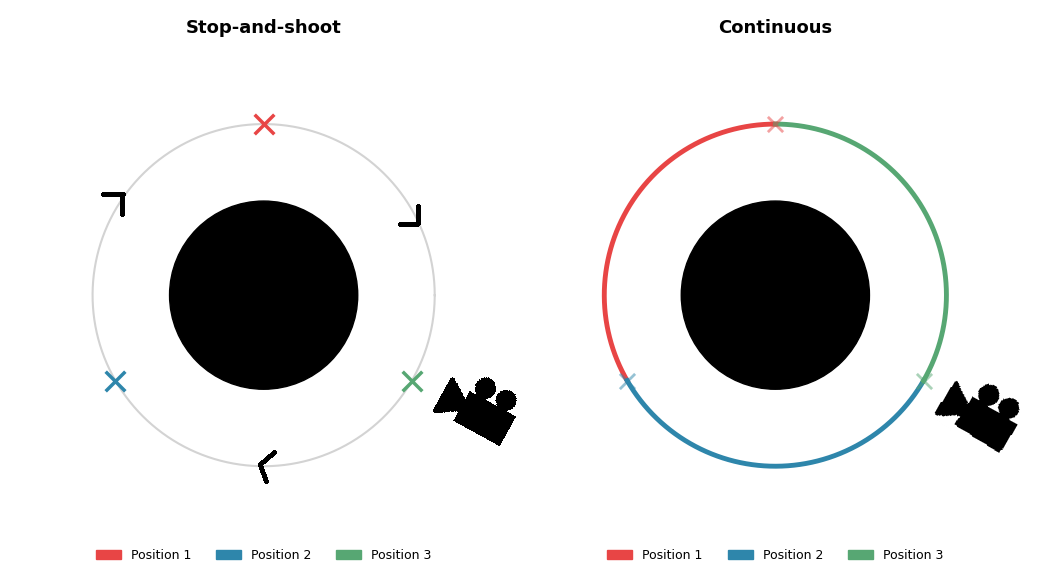
\includegraphics[width=1.2\textwidth]{continous_diagram.png}
    \end{adjustwidth}
    \caption{Top-down view illustrating the difference between step-and-shoot and continuous scanning. In step-and-shoot mode the sample is stationary during each exposure (discrete coloured wedges). In continuous mode the sample rotates throughout, and each projection integrates over a swept angular interval (extended coloured arcs).}
    \label{fig:continous_illu}
\end{figure}

\subsection{Implications for Dynamic Imaging}
\label{subsec:cont_dynamic_implications}

For static samples, the total angular coverage and photon dose can be matched between the two modes, but the projections themselves differ geometrically. Each continuous-scan projection integrates over an angular interval rather than capturing a single angle, producing a blurred projection that carries the same total information in a different form. When the forward model correctly accounts for this integration, the reconstructions can converge to equivalent quality. The practical advantage of continuous rotation is that eliminating motor overhead allows more projections to be collected per unit time, or the same number of projections to be collected in a shorter total scan duration.

For dynamic samples the comparison is more nuanced. The temporal resolution of a step-and-shoot scan is limited by the time required to collect enough projections for a well-conditioned reconstruction, which includes both the exposure time and the motor overhead. Continuous rotation removes the motor overhead, so the time between consecutive projections is reduced to the bare exposure time $\tau$. For processes whose characteristic timescale is comparable to or shorter than the step-and-shoot inter-frame interval, this reduction in $\Delta t$ makes previously unresolvable events accessible.

The trade-off is that a reconstruction algorithm which treats continuous-scan projections as single-angle step-and-shoot projections will have a systematic error in its forward model. The magnitude of this error depends on $\Delta\phi$. For small angular sweeps it is negligible, but for large sweeps the mismatch between the assumed single-angle-per-projection geometry and the true angularly integrated geometry introduces visible blurring artefacts in the reconstruction. Correctly accounting for continuous rotation therefore requires a modification to the Beer--Lambert forward model.


\subsection{Continuous-Scan Forward Model}
\label{subsec:cont_forward_theory}

In step-and-shoot mode the intensity recorded at detector pixel $j$ for a projection at angle $\phi$ follows Beer--Lambert's law along a single ray:
%
\begin{equation}
    I_j^{\phi} = I_0 \exp\!\left(-\int_{\mathbf{r}_j^{\phi}} \mu\!\left(\mathbf{r}\right) \mathrm{d}r\right).
    \label{eq:step_shoot_forward}
\end{equation}
%
In continuous rotation mode the sample rotates from $\phi_s$ to $\phi_e = \phi_s + \Delta\phi$ during the exposure. The detector integrates the instantaneous transmitted intensity over this interval. Assuming constant angular velocity and a linear detector response, the recorded intensity is the angular average of the instantaneous Beer--Lambert transmission:
%
\begin{equation}
    I_j^{[\phi_s,\,\phi_e]} = \frac{1}{\Delta\phi} \int_{\phi_s}^{\phi_e}
        I_0 \exp\!\left(-\int_{\mathbf{r}_j^{\phi}} \mu\!\left(\mathbf{r}\right) \mathrm{d}r\right)
    \mathrm{d}\phi.
    \label{eq:continuous_forward_exact}
\end{equation}
%
The inner integral is the standard Beer--Lambert line integral along the ray defined by detector pixel $j$ and source position at angle $\phi$. The outer integral averages these line integrals over all angles in the swept interval. This double integral has no general closed form, because the ray path $\mathbf{r}_j^{\phi}$ changes continuously with $\phi$ and the attenuation field $\mu$ is an arbitrary function of position.

It is instructive to consider the limiting cases. When $\Delta\phi \to 0$, the outer integral collapses to a point evaluation and Equation~\ref{eq:continuous_forward_exact} reduces to the step-and-shoot forward model~\ref{eq:step_shoot_forward}. When $\Delta\phi$ is large, each stored feature vector must represent the average transmission over a wide range of angles, which washes out fine angular detail in the projection and manifests as blurring in the reconstructed volume.


% ─────────────────────────────────────────────────────────────────────────────
\section{Method}
\label{sec:cont_method}
% ─────────────────────────────────────────────────────────────────────────────

\subsection{$K$-Step Midpoint Approximation}
\label{subsec:cont_kstep}

The exact continuous-scan integral~\ref{eq:continuous_forward_exact} is approximated by dividing the swept angular interval $[\phi_s, \phi_e]$ into $K$ equal sub-intervals and evaluating the Beer--Lambert transmission at the midpoint angle of each sub-interval. This midpoint rule approximation gives a predicted intensity of
%
\begin{equation}
    \hat{I}_j^{[\phi_s,\,\phi_e]} = \frac{1}{K} \sum_{k=0}^{K-1}
        I_0 \exp\!\left(-\sum_{p=1}^{P} \muhat\!\left(\mathbf{r}_p^{\phi_k},\, t_j\right) \Delta s\right),
    \qquad
    \phi_k = \phi_s + \left(k + \tfrac{1}{2}\right)\frac{\Delta\phi}{K},
    \label{eq:continuous_forward_discrete}
\end{equation}
%
where $\mathbf{r}_p^{\phi_k}$ are the $P$ equidistant sample points along the ray cast through detector pixel $j$ at sub-step angle $\phi_k$, $\Delta s$ is the step size between adjacent sample points, and $t_j$ is the timestamp assigned to the projection. The approximation quality improves monotonically with $K$. Setting $K = 1$ places a single ray at the midpoint angle $(\phi_s + \phi_e)/2$, which is equivalent to the step-and-shoot forward model with a possible angular error of up to $\Delta\phi/2$. Increasing $K$ reduces the maximum angular error per sub-step to $\Delta\phi / (2K)$ and makes the outer sum converge to the true integral as $K \to \infty$.

The computational cost of the forward pass scales linearly with $K$, since each of the $K$ sub-steps requires an independent set of $P$ network evaluations per ray. The total number of network evaluations per projection per training step is therefore $K \times P$, compared to $P$ for the standard step-and-shoot pass.

The choice of $K$ for each dataset is guided empirically by the matched-pair design of the experiments, in which two configurations with the same effective sub-step angle are compared directly. If the approximation is adequate, the matched pair should produce equivalent reconstruction quality regardless of which combination of $\Delta\phi$ and $K$ was used to reach that sub-step. This empirical equivalence is a more direct validation of $K$ sufficiency than a theoretical convergence analysis, because it reflects the actual reconstruction error on real data rather than the error of the quadrature rule for an abstract smooth integrand.

\subsection{Training Step Implementation}
\label{subsec:cont_implementation}

The $K$-step forward pass increases the number of network evaluations per training step by a factor of $K$. This also multiplies the activation memory, because all intermediate values needed for backpropagation must be kept alive until the loss gradient is computed. For large $K$ or large batch sizes, holding the computation graphs for all $K$ sub-steps simultaneously can exceed GPU memory capacity. \NeCTv{} provides two implementations of the training step that make opposite trade-offs between memory and compute, selected by the \texttt{memvstime} flag.

\paragraph{Time-efficient mode.}
All $K$ sub-steps are executed in a single forward pass with gradient tracking active throughout. The predicted intensities $\hat{I}_j$ accumulate live computation graphs from all $K$ sub-steps, the loss is evaluated once, and \texttt{backward()} is called on the loss to produce all parameter gradients in one pass. This requires only $K$ forward evaluations and one backward pass, but the activation memory scales as $\mathcal{O}(K)$ because every sub-step graph must coexist until backpropagation completes. Algorithm~\ref{alg:memvstime_true} gives the pseudocode.

\begin{algorithm}[htbp]
\caption{Continuous-Scan Training Step --- Time-Efficient}
\label{alg:memvstime_true}
\begin{algorithmic}[1]
\Require Interval $[\phi_s, \phi_e]$, steps $K$, timestamp $t_j$, measured projection $I_j$
\State $\hat{I}_j \gets 0$,\quad $\bar{I}_j \gets 0$,\quad $\delta\phi \gets (\phi_e - \phi_s)/K$
\For{$k = 0,\ldots,K-1$} \hfill\Comment{gradient tracking active}
    \State $\phi_k \gets \phi_s + (k+\tfrac{1}{2})\,\delta\phi$
    \State Sample rays at $\phi_k$; query $f_{\boldsymbol{\theta}}$ at all sample points
    \State $\hat{I}_j \gets \hat{I}_j + \tfrac{1}{K}\,\mathcal{R}(f_{\boldsymbol{\theta}},\,\phi_k,\,t_j)$;\quad $\bar{I}_j \gets \bar{I}_j + I_j/K$
\EndFor
\State $\mathcal{L} \gets \mathrm{Loss}(\hat{I}_j,\,\bar{I}_j)$;\quad \textbf{backward}$(\mathcal{L})$;\quad \textbf{optimizer.step}()
\end{algorithmic}
\end{algorithm}

\paragraph{Memory-efficient mode.}
The training step is split into two passes. In the first pass all $K$ sub-steps are executed without gradient tracking, accumulating only the scalar predicted intensities $\hat{I}_j$ and caching the ray sample coordinates for each sub-step. The loss is then computed treating $\hat{I}_j$ as a leaf variable, giving the gradient $g = \partial\mathcal{L}/\partial\hat{I}_j$ without touching any model parameters. In the second pass each sub-step is replayed individually with gradient tracking enabled. The contribution of sub-step $k$ is scaled by $g$ and backpropagated, immediately discarding the computation graph before the next sub-step begins. Because at most one sub-step graph exists at any moment, the activation memory overhead is $\mathcal{O}(1)$ with respect to $K$. The cost is $2K$ forward evaluations instead of $K$, doubling the compute relative to time-efficient mode. Algorithm~\ref{alg:memvstime_false} gives the pseudocode.

\begin{algorithm}[htbp]
\caption{Continuous-Scan Training Step --- Memory-Efficient}
\label{alg:memvstime_false}
\begin{algorithmic}[1]
\Require Interval $[\phi_s, \phi_e]$, steps $K$, timestamp $t_j$, measured projection $I_j$
\State $\hat{I}_j \gets 0$,\quad $\bar{I}_j \gets 0$,\quad $\mathcal{C} \gets [\,]$,\quad $\delta\phi \gets (\phi_e - \phi_s)/K$
\For{$k = 0,\ldots,K-1$} \hfill\Comment{Pass 1: no gradient tracking}
    \State $\phi_k \gets \phi_s + (k+\tfrac{1}{2})\,\delta\phi$;\quad cache sample coordinates $\mathbf{r}^{(k)}$ in $\mathcal{C}$
    \State \textbf{with} \texttt{no\_grad}:\quad $c_k \gets \mathcal{R}(f_{\boldsymbol{\theta}},\,\phi_k,\,t_j)$
    \State $\hat{I}_j \gets \hat{I}_j + c_k/K$;\quad $\bar{I}_j \gets \bar{I}_j + I_j/K$
\EndFor
\State Treat $\hat{I}_j$ as leaf;\quad $\mathcal{L} \gets \mathrm{Loss}(\hat{I}_j,\,\bar{I}_j)$;\quad $g \gets \partial\mathcal{L}/\partial\hat{I}_j$
\For{$k = 0,\ldots,K-1$} \hfill\Comment{Pass 2: replay with gradient tracking}
    \State Restore $\mathbf{r}^{(k)}$ from $\mathcal{C}$;\quad $c_k \gets \mathcal{R}(f_{\boldsymbol{\theta}},\,\phi_k,\,t_j)$
    \State \textbf{backward}$((c_k/K)\cdot g)$ \hfill\Comment{accumulate $\nabla_{\boldsymbol{\theta}}\mathcal{L}$; discard graph}
\EndFor
\State \textbf{optimizer.step}()
\end{algorithmic}
\end{algorithm}

In practice the memory-efficient mode makes $K$ a free parameter that can be increased without GPU memory becoming the bottleneck, at the cost of longer training time per step. The time-efficient mode is preferable when $K$ is small and activation memory is not a concern.


\subsection{Hyperparameters and Training Protocol}
\label{subsec:cont_training}

The static experiments use the standard NeCT static model, a single 3D \texttt{xyz} hash encoder with the baseline configuration ($L = 23$, $\log_2 T = 23$, $F = 4$), as described in \cref{subsec:nect_static}. The dynamic experiments use two encoder configurations. The memory-efficient training mode is run with the NeCT QuadCubes baseline, which fits within GPU memory because its $\mathcal{O}(1)$ activation overhead is independent of $K$. The time-efficient mode is run with \MixedCubes{}, whose smaller baseline memory footprint allows it to accommodate the $\mathcal{O}(K)$ activation overhead at higher accumulation steps without exceeding GPU memory. The combination of both encoder architectures and both training modes was necessary to cover the full range of $K$ values tested in the dynamic experiments. The training protocol follows the standard NeCT setup, with the Adam optimiser with a linear warm-up followed by cosine decay, a batch size of $5 \times 10^6$ ray sample points per step, and the adaptive ray-marching schedule that increases $P$ from 100 to $1.5 \times \max(N_\mathrm{detector})$ over the first 30\% of training. The only modification to the training loop is the replacement of the single Beer--Lambert evaluation per projection with the $K$-step averaged forward pass described above.


% ─────────────────────────────────────────────────────────────────────────────
\section{Experiments: Static Validation}
\label{sec:cont_static}
% ─────────────────────────────────────────────────────────────────────────────

The static experiment validates the continuous-scan forward model in a setting where the ground truth is known precisely and the dynamic component of the reconstruction is absent. Because the sample does not change, any degradation in reconstruction quality relative to the ground truth can be attributed entirely to the angular blurring from the continuous acquisition, and any improvement from increasing $K$ can be attributed entirely to the improved accuracy of the forward model approximation.

\subsection{Dataset}
\label{subsec:cont_static_dataset}

The static dataset uses the same Bentheimer sandstone sample as the encoder experiments, scanned without fluid invasion so that the attenuation field is constant throughout. Three independent scans were acquired of the same physical sample, each covering one full single rotation of $360\degree$. The first is a step-and-shoot acquisition with 1400 projections and serves as the ground truth reference, reconstructed with the standard NeCT static model to produce a high-quality 3D volume. The remaining two are continuous-scan acquisitions at 360 and 100 projections respectively, spanning a range of angular step sizes. The standard NeCT static model is used for all reconstructions, with a single 3D \texttt{xyz} hash encoder and no temporal encoder.

\begin{table}[h]
    \centering
    \caption{Static continuous-scan dataset configurations. The angular step $\Delta\phi$ is $360\degree$ divided by the number of projections. Each configuration is reconstructed with accumulation steps $K \in \{1, 2, 3, 4, 6\}$.}
    \label{tab:static_cont_configs}
    \begin{tabular}{ccc}
        \toprule
        Projections & $\Delta\phi$ (degrees) & Effective sub-step $\Delta\phi / K$ at $K = \{1, 2, 3, 4, 6\}$ (degrees) \\
        \midrule
        360  & 1.00 & 1.00,\ \ 0.50,\ \ 0.33,\ \ \ 0.25,\ \ \ 0.17  \\
        100  & 3.60 & 3.60,\ \ 1.80,\ \ 1.20,\ \ \ 0.90,\ \ \ 0.60  \\
        \bottomrule
    \end{tabular}
\end{table}

Several effective sub-step sizes coincide across the two continuous-scan configurations, as shown in Table~\ref{tab:static_cont_configs}. For example, 360 projections at $K = 4$ gives $0.25\degree$ per sub-step, nearly identical to the $0.26\degree$ step size of the step-and-shoot ground truth. Comparing reconstruction quality across these matched pairs directly tests whether the $K$-step approximation fully compensates for the larger raw angular step or whether some residual information loss persists.

\subsection{Evaluation Metrics}
\label{subsec:cont_static_metrics}

Standard voxel-level metrics such as PSNR and SSIM are not used as the primary evaluation criterion here. Because the continuous-scan acquisitions at different angular step sizes involve slightly different geometric sampling of the volume, reconstructions at larger $\Delta\phi$ can exhibit small spatial offsets relative to the step-and-shoot ground truth. These offsets mean that a blurred, angularly smeared reconstruction can score artificially higher on PSNR or SSIM than a sharper one, simply because its smoothed intensity values happen to align with the ground truth voxel grid more favourably. This is an artefact of the metric rather than a genuine quality advantage, and it would invert the true ranking.

A combined score $S$ is therefore used, built from two quantities that are more robust to this issue. Let $\bar{g}$ denote the mean Sobel gradient magnitude averaged over three fixed slices (XY at $z = 190$, XZ at $y = 152$, YZ at $x = 95$), a no-reference sharpness proxy where higher values indicate better preservation of edges and fine structure. Let $\varepsilon$ denote the MAE against the step-and-shoot ground truth. MAE is included because it remains informative even when small spatial offsets are present, as it measures average absolute deviation rather than pixel-by-pixel correlation. Both quantities are linearly normalised to $[0, 1]$ across all models under comparison:
%
\begin{equation}
    \tilde{g} = \frac{\bar{g} - \bar{g}_{\min}}{\bar{g}_{\max} - \bar{g}_{\min}}, \qquad
    \tilde{\varepsilon} = 1 - \frac{\varepsilon - \varepsilon_{\min}}{\varepsilon_{\max} - \varepsilon_{\min}},
    \label{eq:combined_norm}
\end{equation}
%
so that $\tilde{g} = 1$ for the sharpest reconstruction and $\tilde{\varepsilon} = 1$ for the most accurate. The combined score is their arithmetic mean:
%
\begin{equation}
    S = \frac{\tilde{g} + \tilde{\varepsilon}}{2}.
    \label{eq:combined_score}
\end{equation}
%
The arithmetic mean is used rather than the geometric mean because the geometric mean collapses to zero whenever a model ranks last on either individual component, providing no ranking information in that case. The combined score $S$ is the sole ranking criterion throughout this section.

\subsection{Results}
\label{subsec:cont_static_results}

\begin{figure}[htbp]
    \centering
    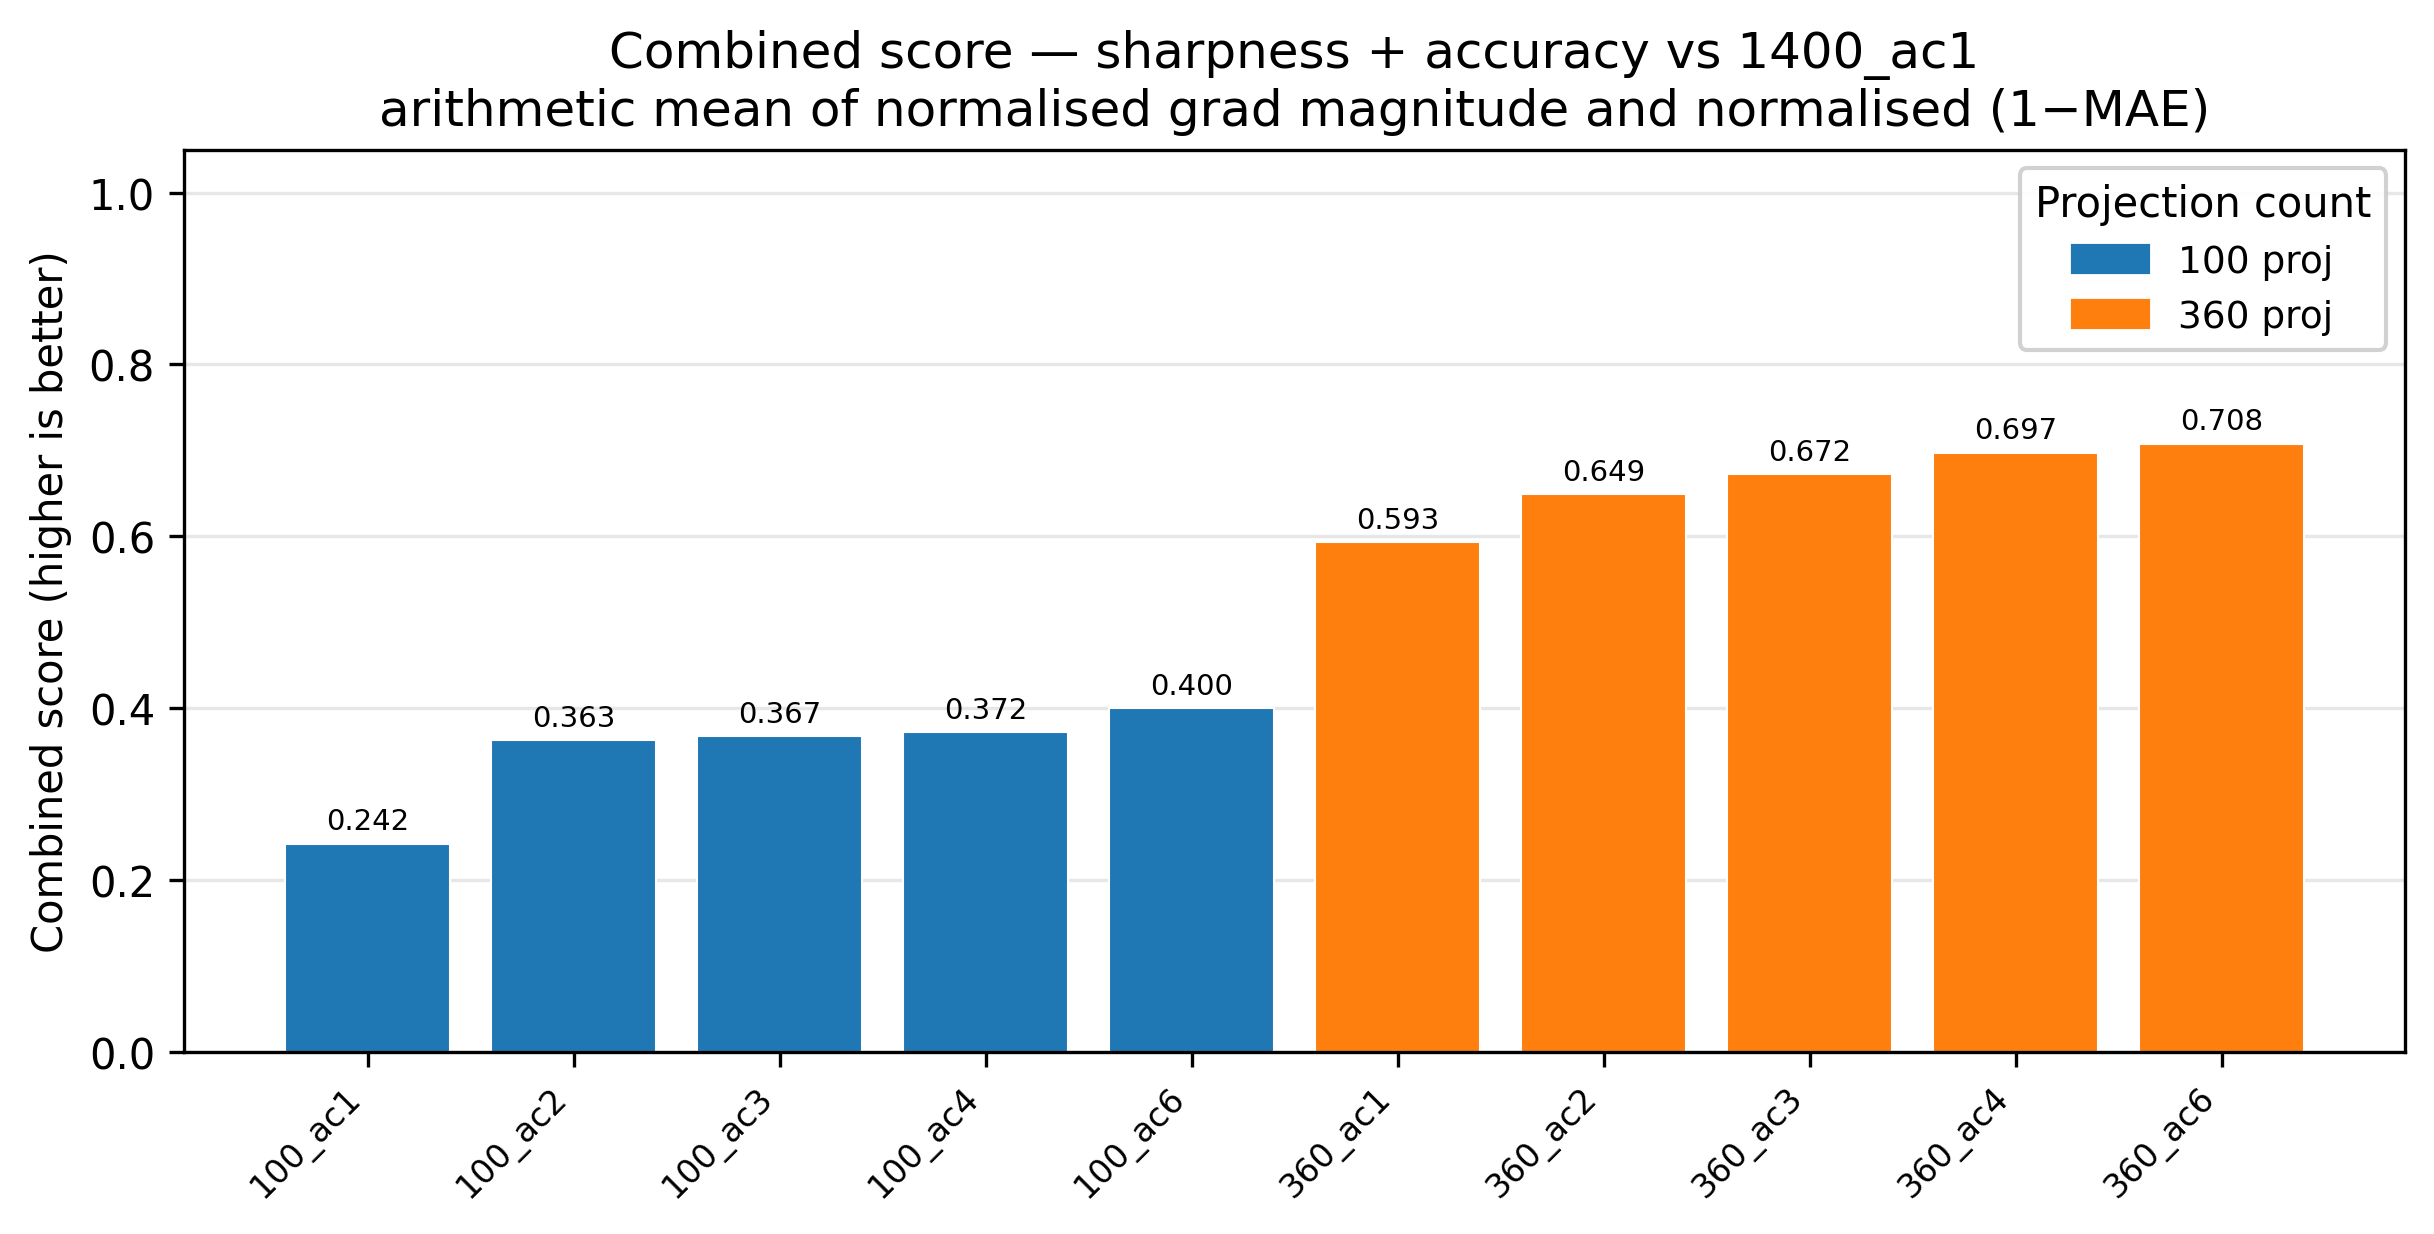
\includegraphics[width=1.1\textwidth]{combined_score.png}
    \caption{Combined score $S$ as a function of accumulation steps $K$ for the 100-projection ($\Delta\phi = 3.60\degree$) and 360-projection ($\Delta\phi = 1.00\degree$) continuous-scan configurations. Higher is better. The 100-projection configuration starts substantially lower at $K = 1$, reflecting the more severe angular blur at the larger angular step, and benefits more from increasing $K$. Both curves increase monotonically.}
    \label{fig:combined_score}
\end{figure}

Figure~\ref{fig:combined_score} shows the combined score as a function of $K$ for both configurations. Figure~\ref{fig:combined_score} shows the combined score as a function of $K$ for both configurations.

For the 100-projection configuration ($\Delta\phi = 3.60\degree$), the $K = 1$ score of 0.242 reflects substantially degraded reconstruction quality. Increasing $K$ produces improvement at every accumulation step, reaching 0.363 at $K = 2$, 0.367 at $K = 3$, 0.372 at $K = 4$, and 0.400 at $K = 6$. The gains are real but diminishing. The jump from $K = 1$ to $K = 2$ is 0.120 points, while the jump from $K = 4$ to $K = 6$ is only 0.028 points. The correction is working, but the rate of improvement decreases with each additional sub-step. At $K = 6$ the combined score reaches 0.400, which remains well below the 360-projection score at $K = 1$ of 0.593. The 100-projection configuration does not approach 360-projection quality at any value of $K$ tested. This is expected because reducing the projection count from 360 to 100 introduces angular undersampling that the $K$-step forward model cannot correct. The correction addresses angular blur within each existing projection but does not add new independent projection angles. The quality ceiling of the 100-projection dataset is set by its projection count, not by its angular step size alone.

It should also be noted that because this is a static sample, continuous scanning provides no additional temporal information over step-and-shoot. The benefit of continuous scanning in a static context is purely about dead-time efficiency, and since the datasets were acquired at fixed projection counts, the experiment isolates the effect of the forward model correction in the absence of any temporal advantage.

For the 360-projection configuration ($\Delta\phi = 1.00\degree$), the $K = 1$ score of 0.593 is already high, and the improvement from increasing $K$ is small. The score rises to 0.649 at $K = 2$, then 0.672 at $K = 3$, 0.697 at $K = 4$, and 0.708 at $K = 6$, a total gain of 0.115 points. The largest single step is again from $K = 1$ to $K = 2$ (0.056 points), with each subsequent step contributing less. At $1\degree$ per projection the angular sweep is already small enough that the forward model mismatch at $K = 1$ is not the dominant source of error, and additional sub-steps return diminishing benefit. Both curves increase monotonically with no decline at higher $K$, confirming that the correction does not introduce new artefacts.

Figures~\ref{fig:static_slices_100} and \ref{fig:static_slices_360} show representative reconstruction slices for each projection count and each accumulation step, paired with the 1400-projection step-and-shoot ground truth.

For the 100-projection configuration the angular blur is clearly visible at $K = 1$. Pore boundaries are smeared and high-attenuation grain edges lose their sharpness relative to the ground truth. The improvement with increasing $K$ is visible in the progressive recovery of edge definition, though the reconstructions remain noticeably softer than the ground truth throughout. The gain is most apparent at the high-intensity regions, where individual grains and their boundaries become progressively better defined as $K$ increases.

For the 360-projection configuration the difference at $K = 1$ is far less pronounced, and the improvement with increasing $K$ is difficult to see in the bulk of the reconstruction. Focusing on the high-intensity regions makes the change more apparent. The sharpest grain edges tighten slightly with each accumulation step, and fine pore boundaries that appear marginally diffuse at $K = 1$ become slightly crisper at $K = 6$. The overall structure is well recovered at all $K$ values, consistent with the combined score results showing only a modest gain across the full range.

\begin{figure}[H]
    \begin{adjustwidth}{-2cm}{0cm}
    \centering
\begin{tabular}{r@{\hspace{6pt}}cc}
& \textbf{100-proj} & \textbf{Ground truth (1400-proj, $K=1$)} \\[4pt]
\toprule
\addlinespace[4pt]
\texttt{Accumulation steps = 1} &
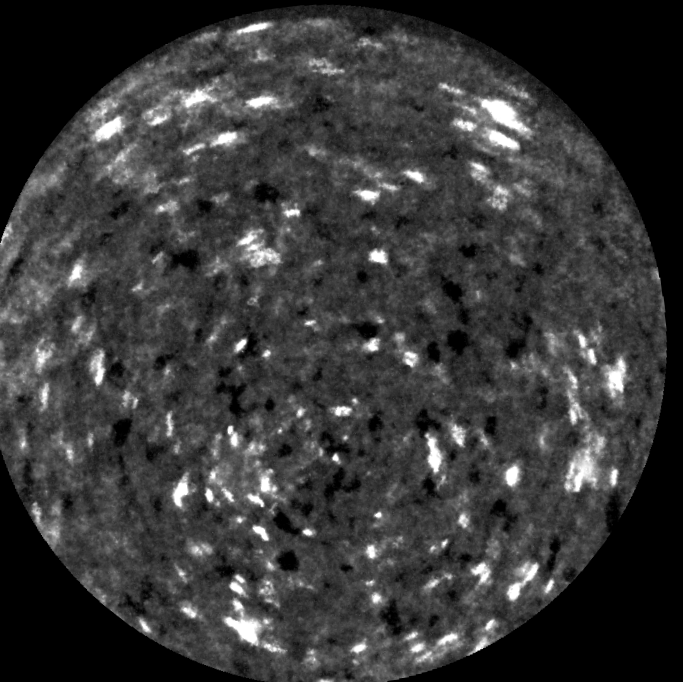
\includegraphics[width=0.34\textwidth]{100_ac1.png} &
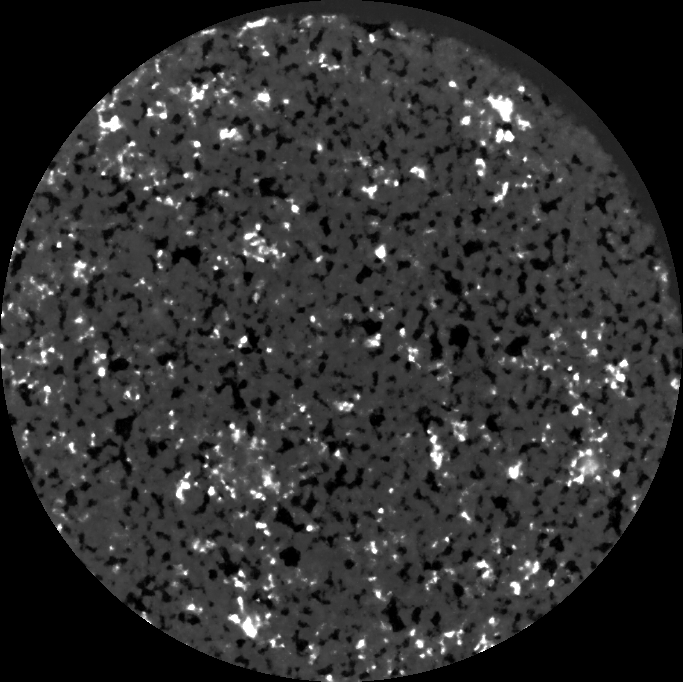
\includegraphics[width=0.34\textwidth]{1400_ac1.png} \\
\addlinespace[2pt]
\texttt{Accumulation steps = 2} &
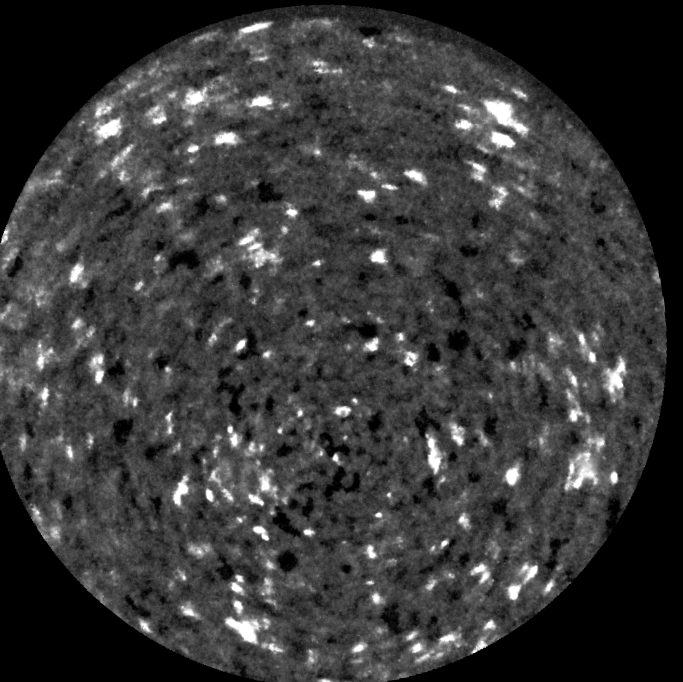
\includegraphics[width=0.34\textwidth]{100_ac2.png} &
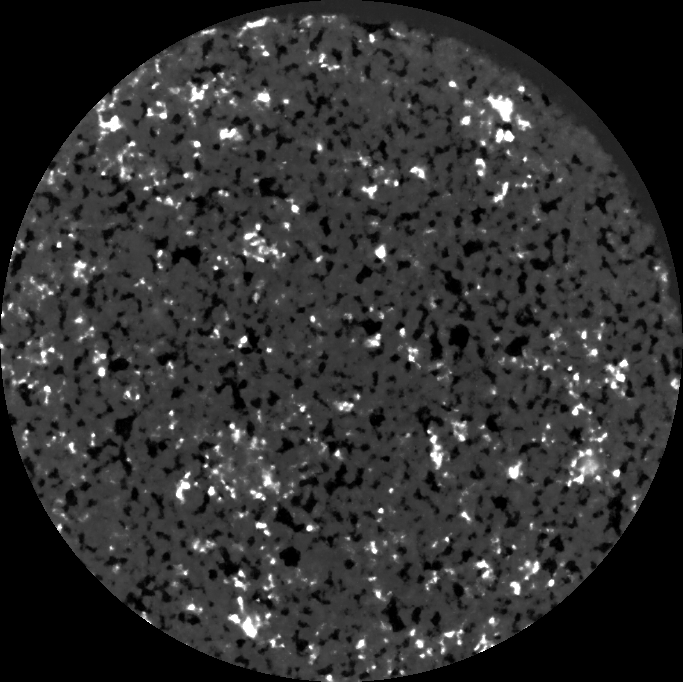
\includegraphics[width=0.34\textwidth]{1400_ac1.png} \\
\addlinespace[2pt]
\texttt{Accumulation steps = 3} &
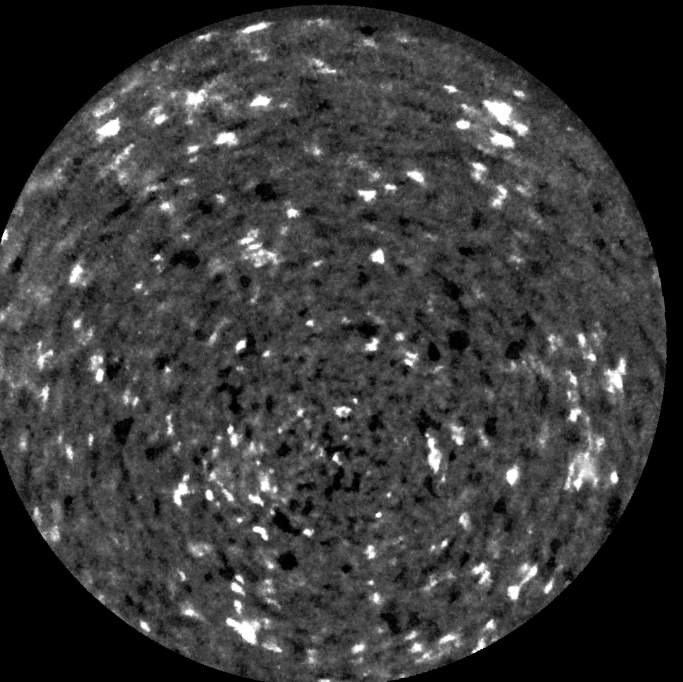
\includegraphics[width=0.34\textwidth]{100_ac3.png} &
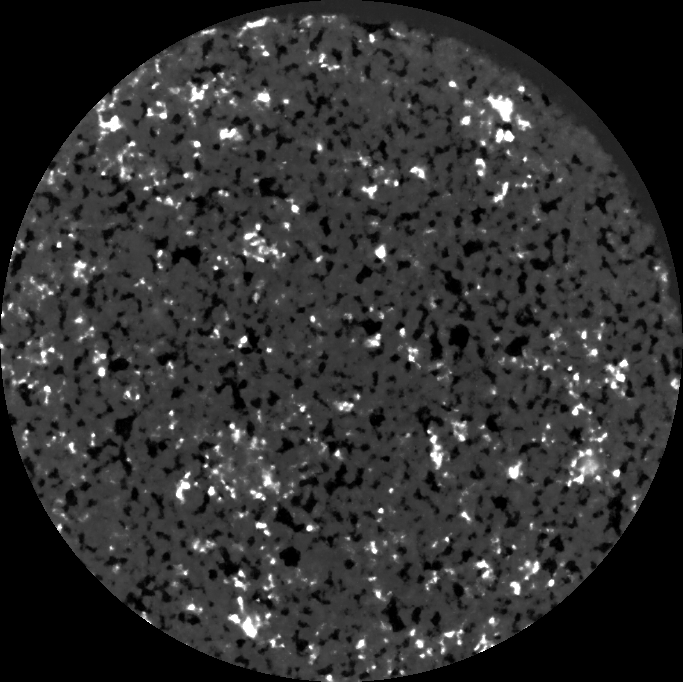
\includegraphics[width=0.34\textwidth]{1400_ac1.png} \\
\addlinespace[2pt]
\texttt{Accumulation steps = 4} &
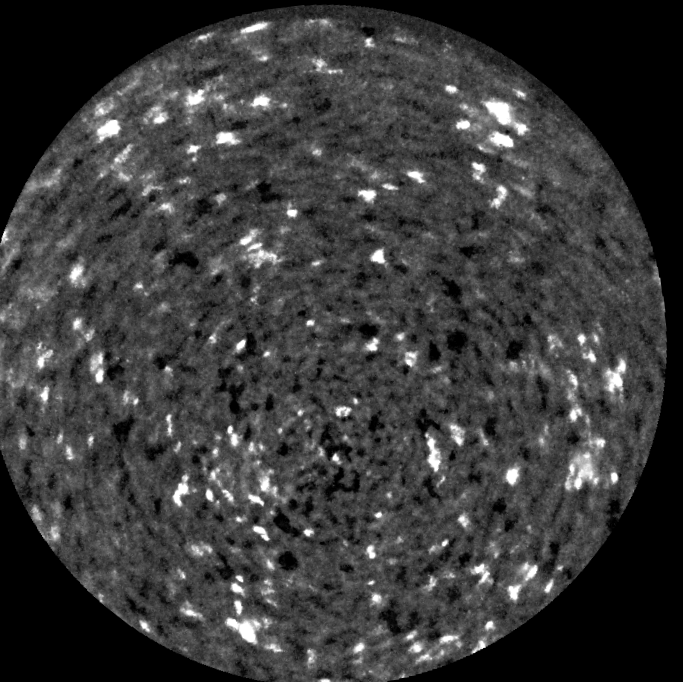
\includegraphics[width=0.34\textwidth]{100_ac4.png} &
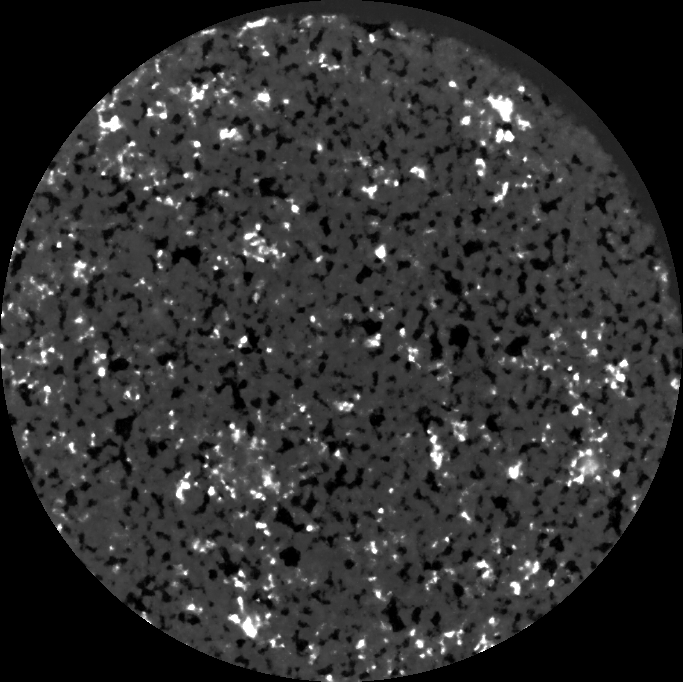
\includegraphics[width=0.34\textwidth]{1400_ac1.png} \\
\addlinespace[2pt]
\texttt{Accumulation steps = 6} &
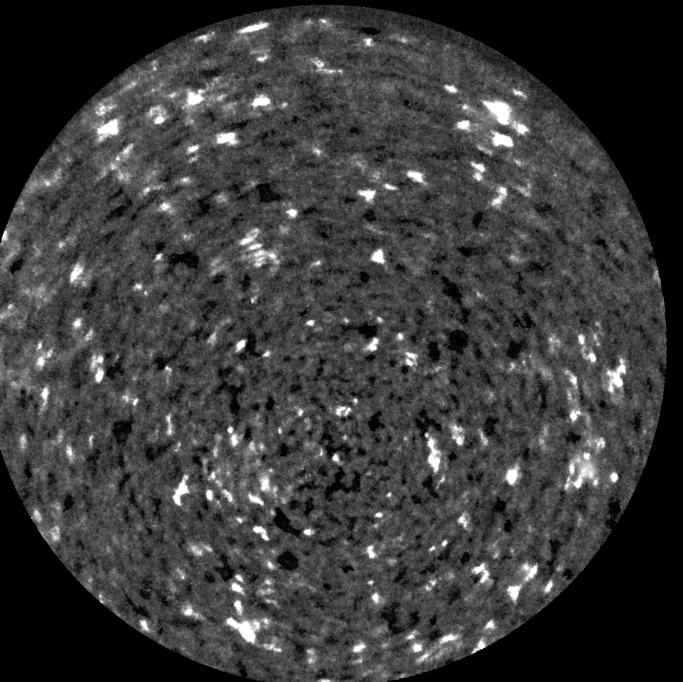
\includegraphics[width=0.34\textwidth]{100_ac6.png} &
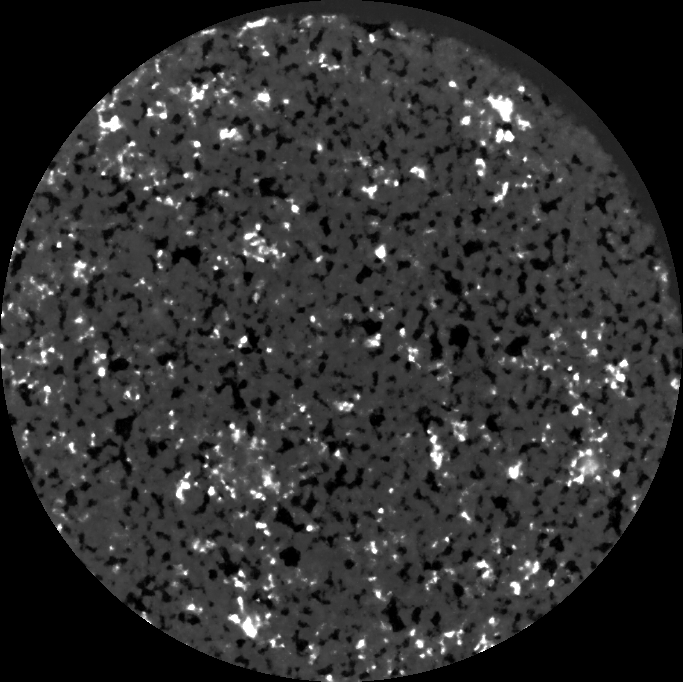
\includegraphics[width=0.34\textwidth]{1400_ac1.png} \\
\end{tabular}
\caption{Reconstruction slice comparisons for the 100-projection continuous-scan configuration ($\Delta\phi = 3.60\degree$) at each accumulation step $K$, paired with the 1400-projection step-and-shoot ground truth. Row labels indicate the configuration.}
\label{fig:static_slices_100}
    \end{adjustwidth}
\end{figure}

\begin{figure}[H]
    \begin{adjustwidth}{-2cm}{0cm}
    \centering
\begin{tabular}{r@{\hspace{6pt}}cc}
& \textbf{360-proj} & \textbf{Ground truth (1400-proj, $K=1$)} \\[4pt]
\toprule
\addlinespace[4pt]
\texttt{Accumulation steps = 1} &
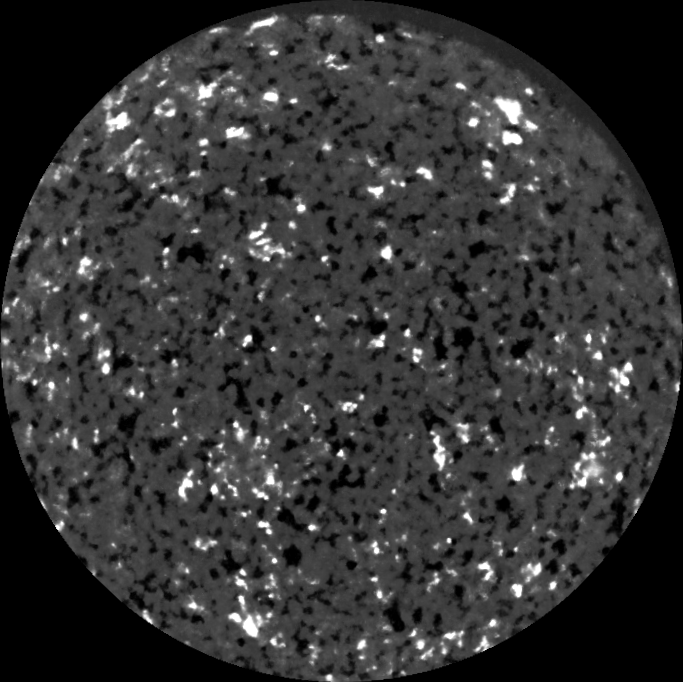
\includegraphics[width=0.34\textwidth]{360_ac1.png} &
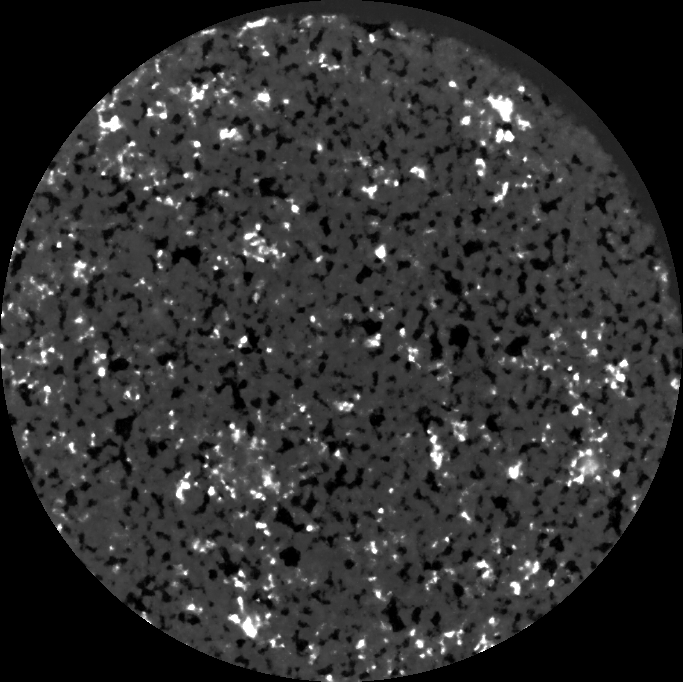
\includegraphics[width=0.34\textwidth]{1400_ac1.png} \\
\addlinespace[2pt]
\texttt{Accumulation steps = 2} &
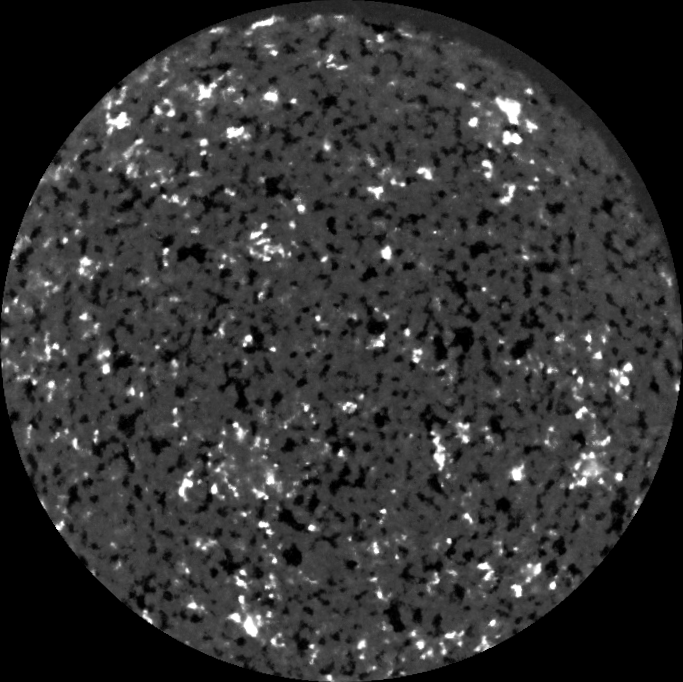
\includegraphics[width=0.34\textwidth]{360_ac2.png} &
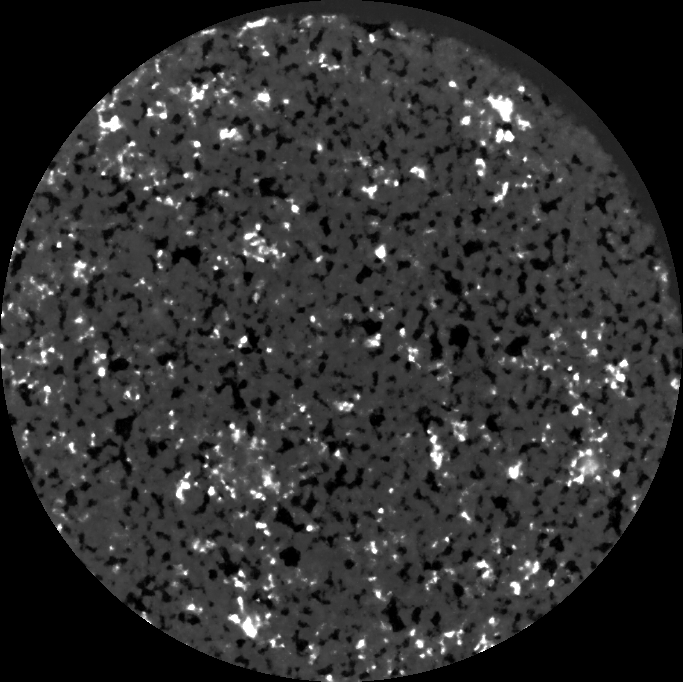
\includegraphics[width=0.34\textwidth]{1400_ac1.png} \\
\addlinespace[2pt]
\texttt{Accumulation steps = 3} &
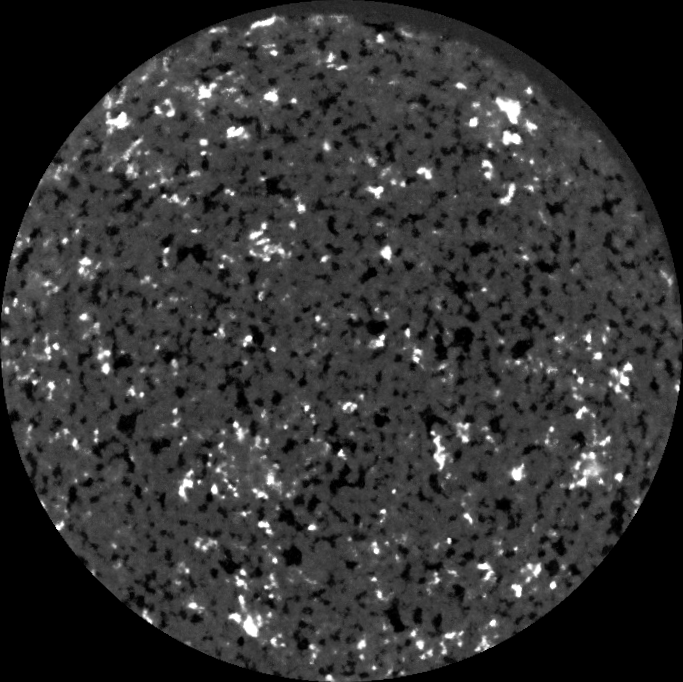
\includegraphics[width=0.34\textwidth]{360_ac3.png} &
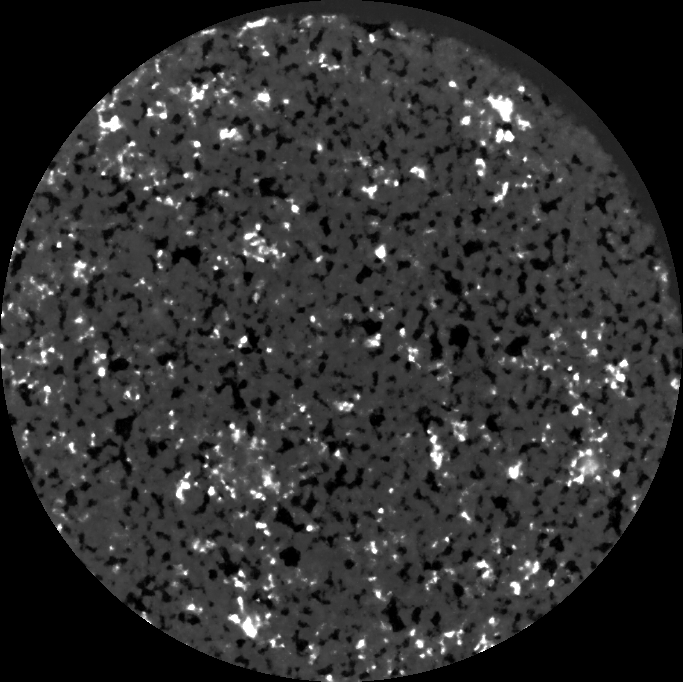
\includegraphics[width=0.34\textwidth]{1400_ac1.png} \\
\addlinespace[2pt]
\texttt{Accumulation steps = 4} &
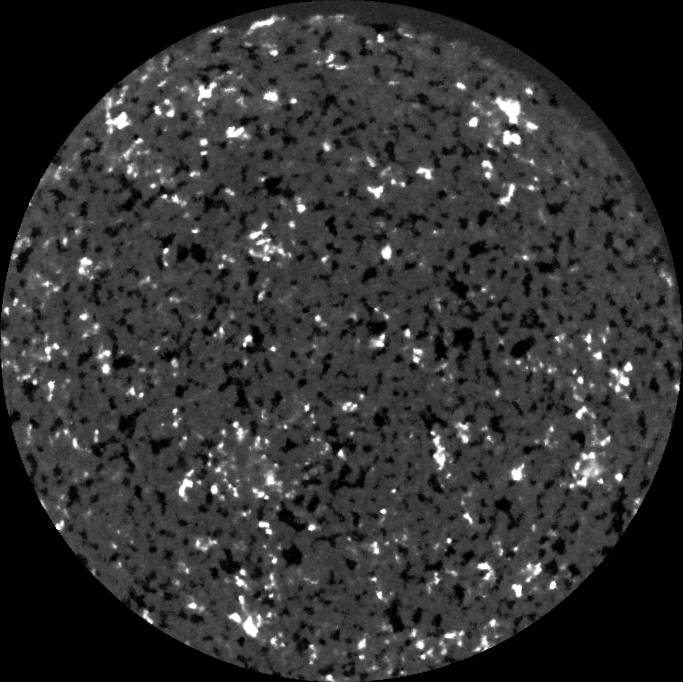
\includegraphics[width=0.34\textwidth]{360_ac4.png} &
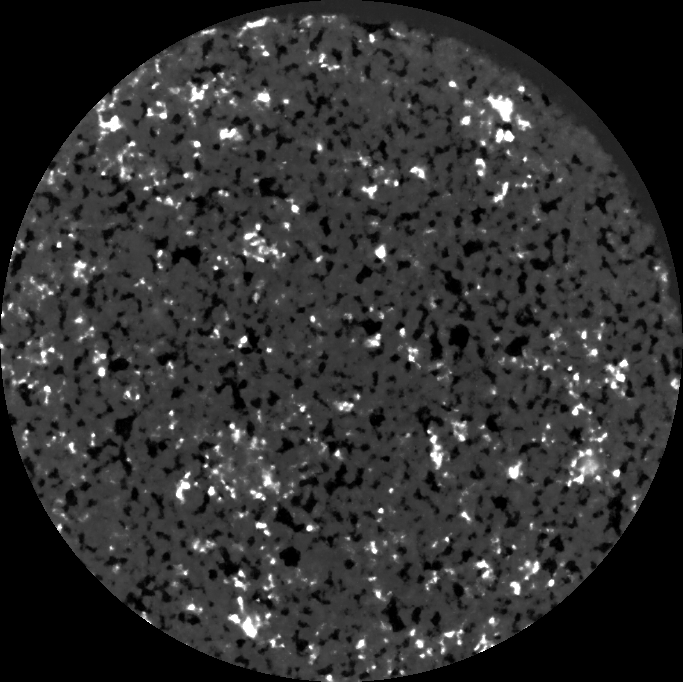
\includegraphics[width=0.34\textwidth]{1400_ac1.png} \\
\addlinespace[2pt]
\texttt{Accumulation steps = 6} &
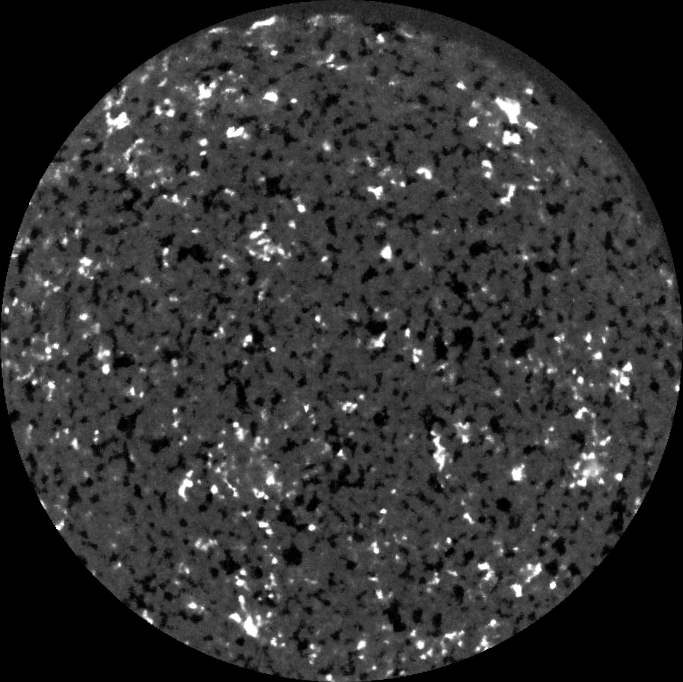
\includegraphics[width=0.34\textwidth]{360_ac6.png} &
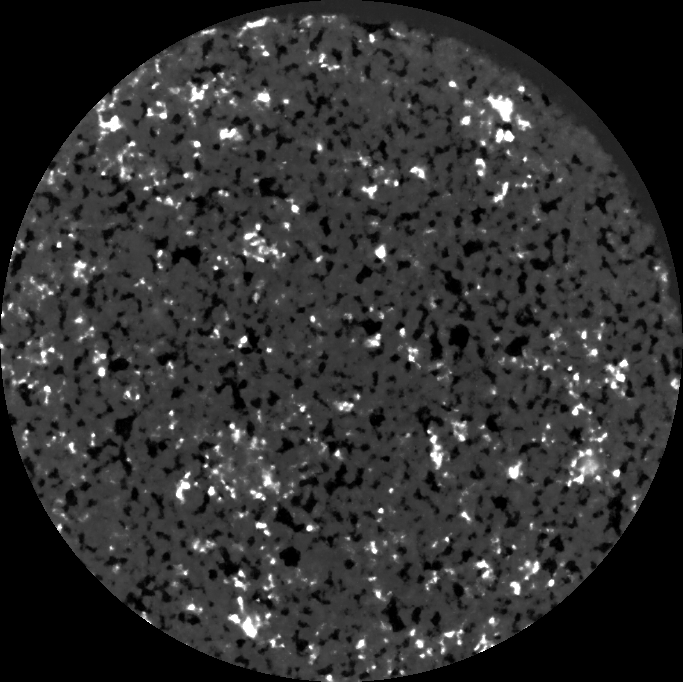
\includegraphics[width=0.34\textwidth]{1400_ac1.png} \\
\end{tabular}
    \end{adjustwidth}
\caption{Reconstruction slice comparisons for the 360-projection continuous-scan configuration ($\Delta\phi = 1.00\degree$) at each accumulation step $K$, paired with the 1400-projection step-and-shoot ground truth.}
\label{fig:static_slices_360}
\end{figure}


\subsection{Why the Improvement is Limited: Sub-angle Degeneracy}
\label{subsec:cont_decoupling}

The gains in the static experiment are real but modest, and understanding why requires examining how the $K$-step model learns from projections acquired in a single revolution.

The $K$-step approximation divides each projection's swept angular interval into $K$ sub-rays and evaluates the Beer--Lambert integral at each sub-angle midpoint. The predicted intensity is the average of these $K$ sub-ray transmissions. With only one revolution, each sub-angle position within a projection appears exclusively in that one projection. The model receives one averaged measurement per projection interval, and the individual contributions from each sub-angle within that interval are completely indistinguishable from one another.

Figures~\ref{fig:subangle_1} and~\ref{fig:subangle_2} illustrate this. A projection sweeping from $0\degree$ to $60\degree$ with $K = 3$ places sub-rays at $a_1 = 10\degree$, $a_2 = 30\degree$, and $a_3 = 50\degree$. The model receives one scalar measurement $S_A$. All three sub-angle contributions are assigned equal weight in the averaged constraint, and the true signal at those angles, which may vary substantially, remains hidden. There is no way to separate the contributions from a single measurement.

\begin{figure}[htbp]
    \begin{adjustwidth}{-1cm}{0cm}
    \centering
    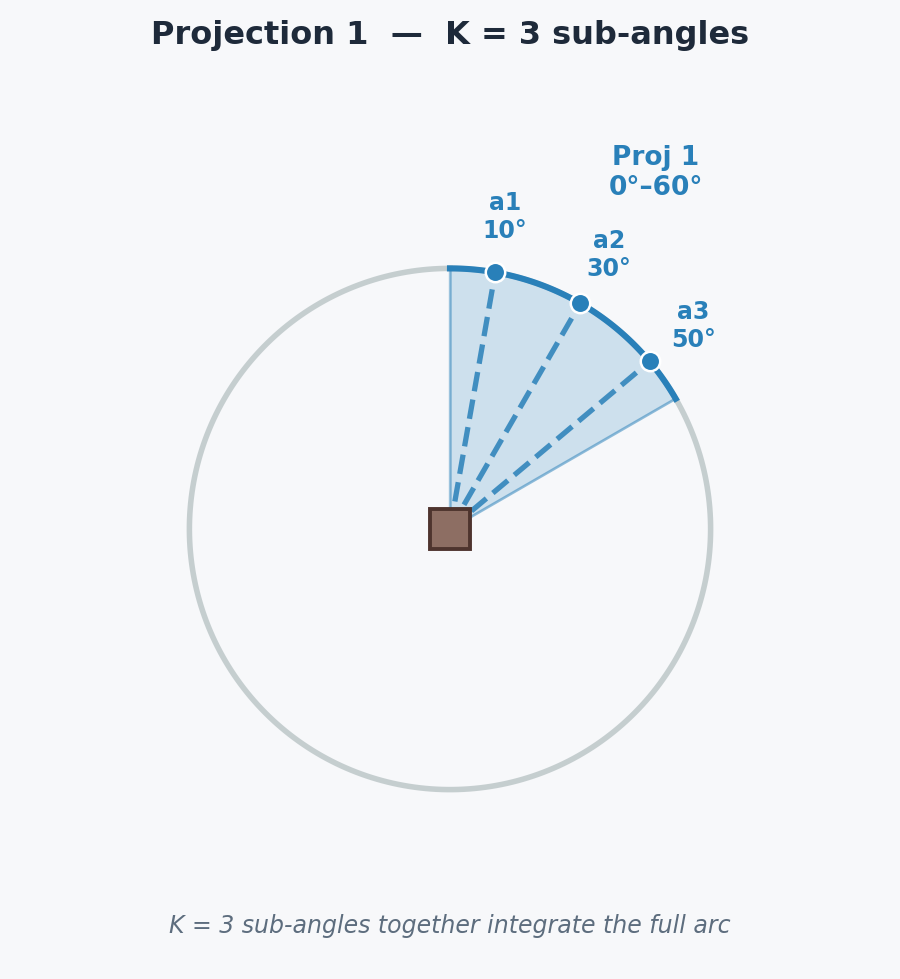
\includegraphics[width=1.15\textwidth]{fig_subangle_1.png}
    \end{adjustwidth}
    \caption{Top-down view of one continuous-scan projection sweeping from $0\degree$ to $60\degree$. Three sub-angle midpoints are placed at $a_1 = 10\degree$, $a_2 = 30\degree$, and $a_3 = 50\degree$ ($K = 3$). The coloured wedge represents the angular interval integrated during this exposure.}
    \label{fig:subangle_1}
\end{figure}

\begin{figure}[htbp]
    \begin{adjustwidth}{-1cm}{0cm}
    \centering
    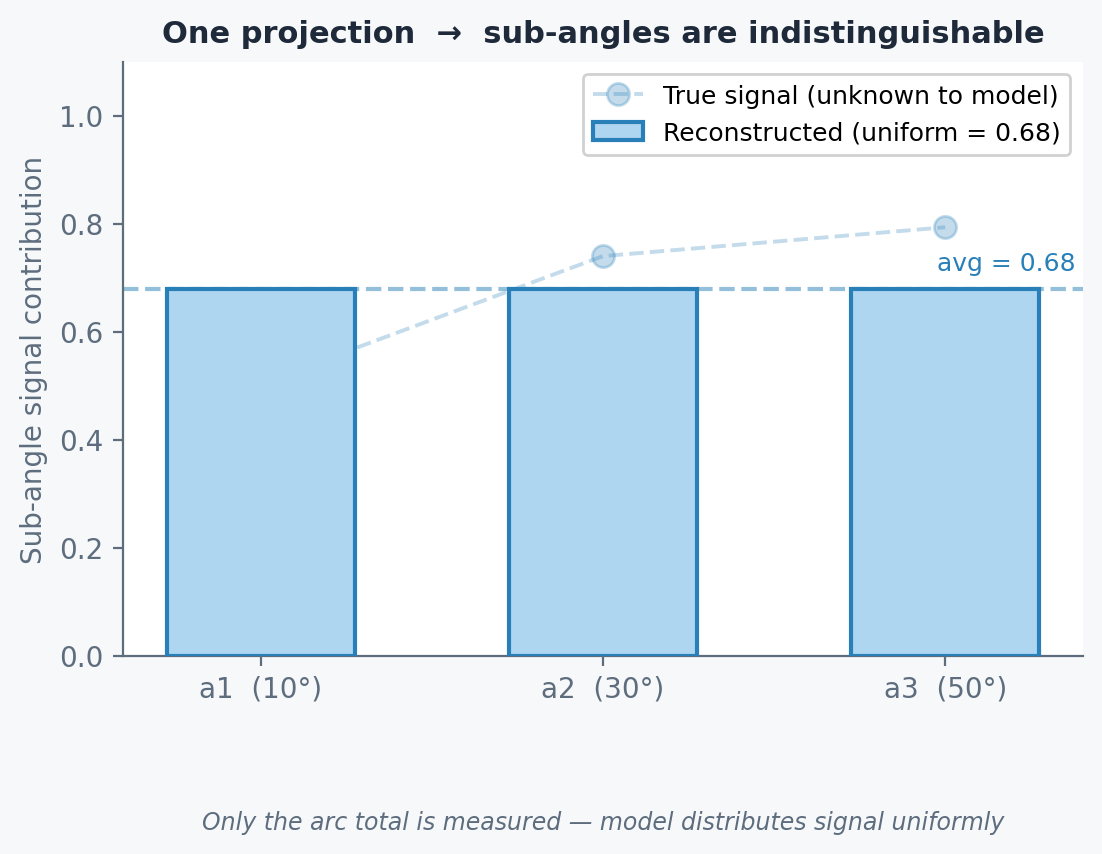
\includegraphics[width=1.15\textwidth]{fig_subangle_2.png}
    \end{adjustwidth}
    \caption{Signal contribution at each sub-angle for a single projection. The three bars for $a_1$, $a_2$, and $a_3$ are all equal, representing the uniform average constraint the model receives from one measurement. The shaded curve in the background shows the true signal at each angle.}
    \label{fig:subangle_2}
\end{figure}

The situation changes when a second projection arrives from a different angular position following the hybrid golden-section scheme. Projection~2 sweeps from $40\degree$ to $100\degree$ with sub-angles at $b_1 = 50\degree$, $b_2 = 70\degree$, and $b_3 = 90\degree$. Critically, $b_1 = a_3 = 50\degree$. This angle now appears in two projections with different neighbours on each side. The two averaged measurements $S_A$ and $S_B$ share a common unknown at $50\degree$, making the system partially constrained in a way the single-projection case was not.

\begin{figure}[htbp]
    \begin{adjustwidth}{-1cm}{0cm}
    \centering
    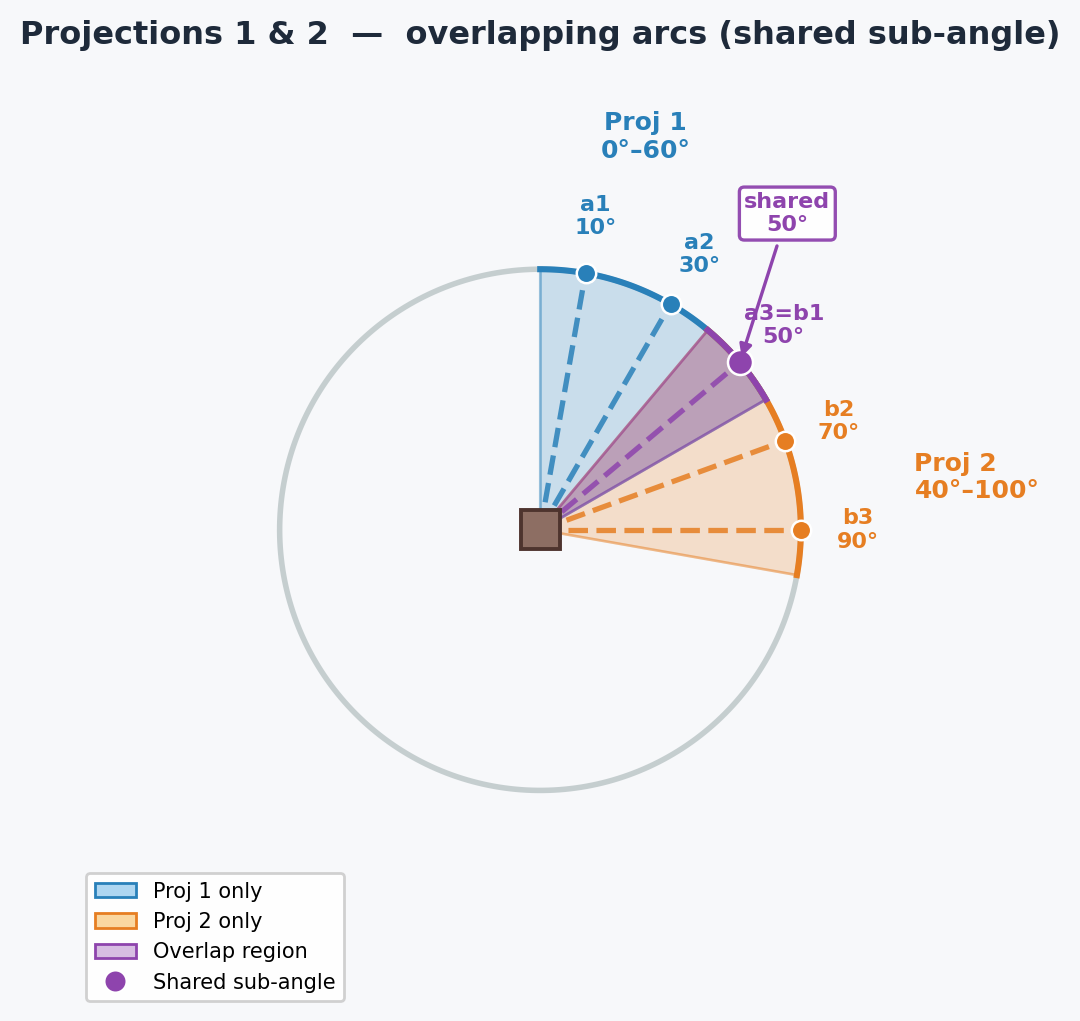
\includegraphics[width=1.15\textwidth]{fig_subangle_3.png}
    \end{adjustwidth}
    \caption{Top-down view of two overlapping continuous-scan projections. Projection~1 (blue) covers $0\degree$--$60\degree$ with sub-angles $a_1 = 10\degree$, $a_2 = 30\degree$, $a_3 = 50\degree$. Projection~2 (orange) covers $40\degree$--$100\degree$ with sub-angles $b_1 = 50\degree$, $b_2 = 70\degree$, $b_3 = 90\degree$. The angle $50\degree$ is shared between $a_3$ and $b_1$.}
    \label{fig:subangle_3}
\end{figure}

\begin{figure}[htbp]
    \begin{adjustwidth}{-1cm}{0cm}
    \centering
    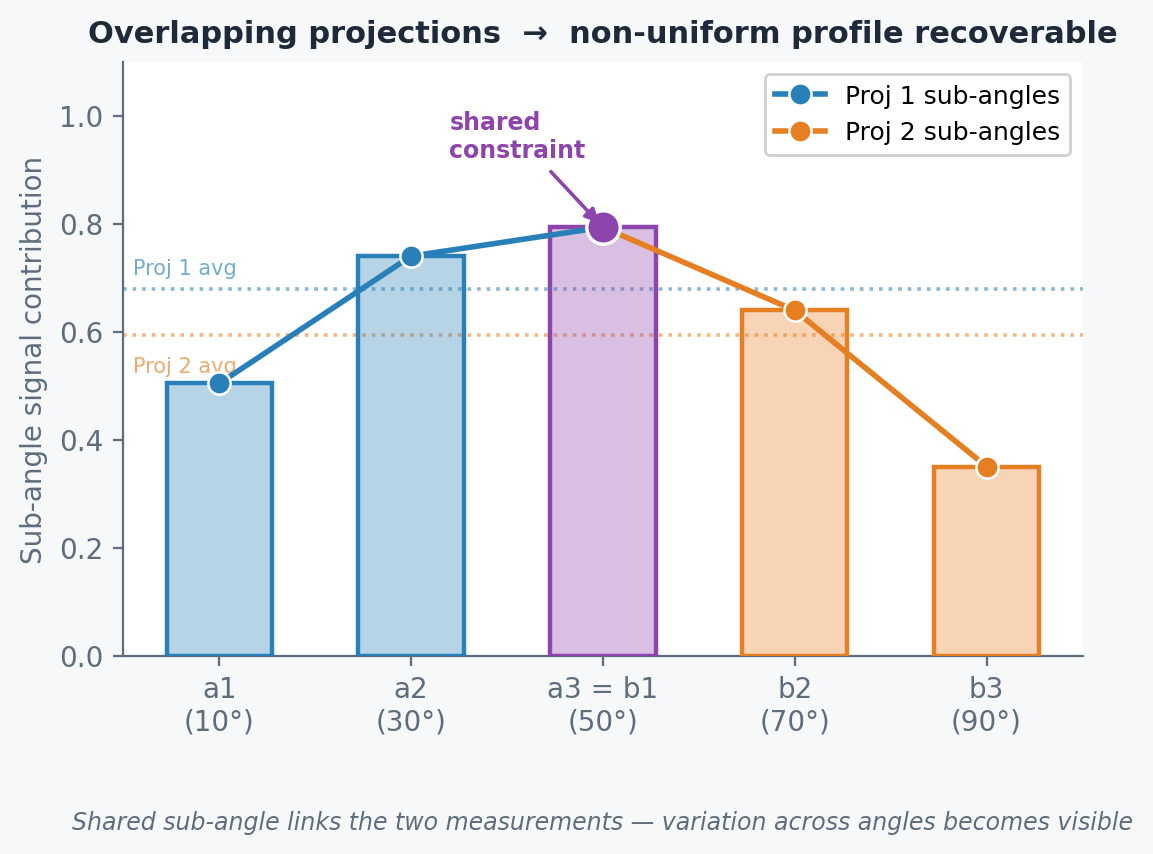
\includegraphics[width=1.15\textwidth]{fig_subangle_4.png}
    \end{adjustwidth}
    \caption{Combined signal bar graph for both projections. At the shared angle $50\degree$ the bar begins to match the true signal curve, showing how the overlapping constraint allows the model to start separating individual sub-angle contributions.}
    \label{fig:subangle_4}
\end{figure}

As additional revolutions accumulate, the golden-angle offset continues to place new sub-angles in the largest remaining gaps. The angular coverage becomes progressively denser and the number of shared sub-angle constraints grows, allowing the model to resolve finer and finer sub-angle structure. This is the mechanism by which a multi-revolution continuous-scan acquisition can genuinely outperform a step-and-shoot acquisition using the same projections. Without multiple revolutions, the sub-angle contributions remain degenerate and the only benefit from increasing $K$ is a better numerical approximation of the angular integral, which explains the modest but real gains observed in the static Bentheimer experiment. The dynamic hourglass experiment was designed to address this limitation by acquiring data across multiple revolutions.


% ─────────────────────────────────────────────────────────────────────────────
\section{Experiments: Dynamic Hourglass}
\label{sec:cont_dynamic}
% ─────────────────────────────────────────────────────────────────────────────

The static experiment revealed that a single-revolution acquisition prevents the sub-angle decoupling mechanism from operating, limiting any improvement from increasing $K$ to better numerical approximation of the angular integral. The dynamic hourglass experiment addresses this directly. The hourglass dataset spans multiple revolutions following the hybrid golden-section scheme, providing the cross-projection sub-angle constraints that the static experiment lacked. Sand flows between two chambers on a timescale of minutes, producing clearly visible structural changes between successive projections while remaining a physically simple system. This experiment therefore tests whether multi-revolution continuous scanning and the $K$-step correction together produce a meaningful improvement in 4D reconstruction quality.

\subsection{Dataset}
\label{subsec:cont_dynamic_dataset}

\begin{figure}[htbp]
    \centering
    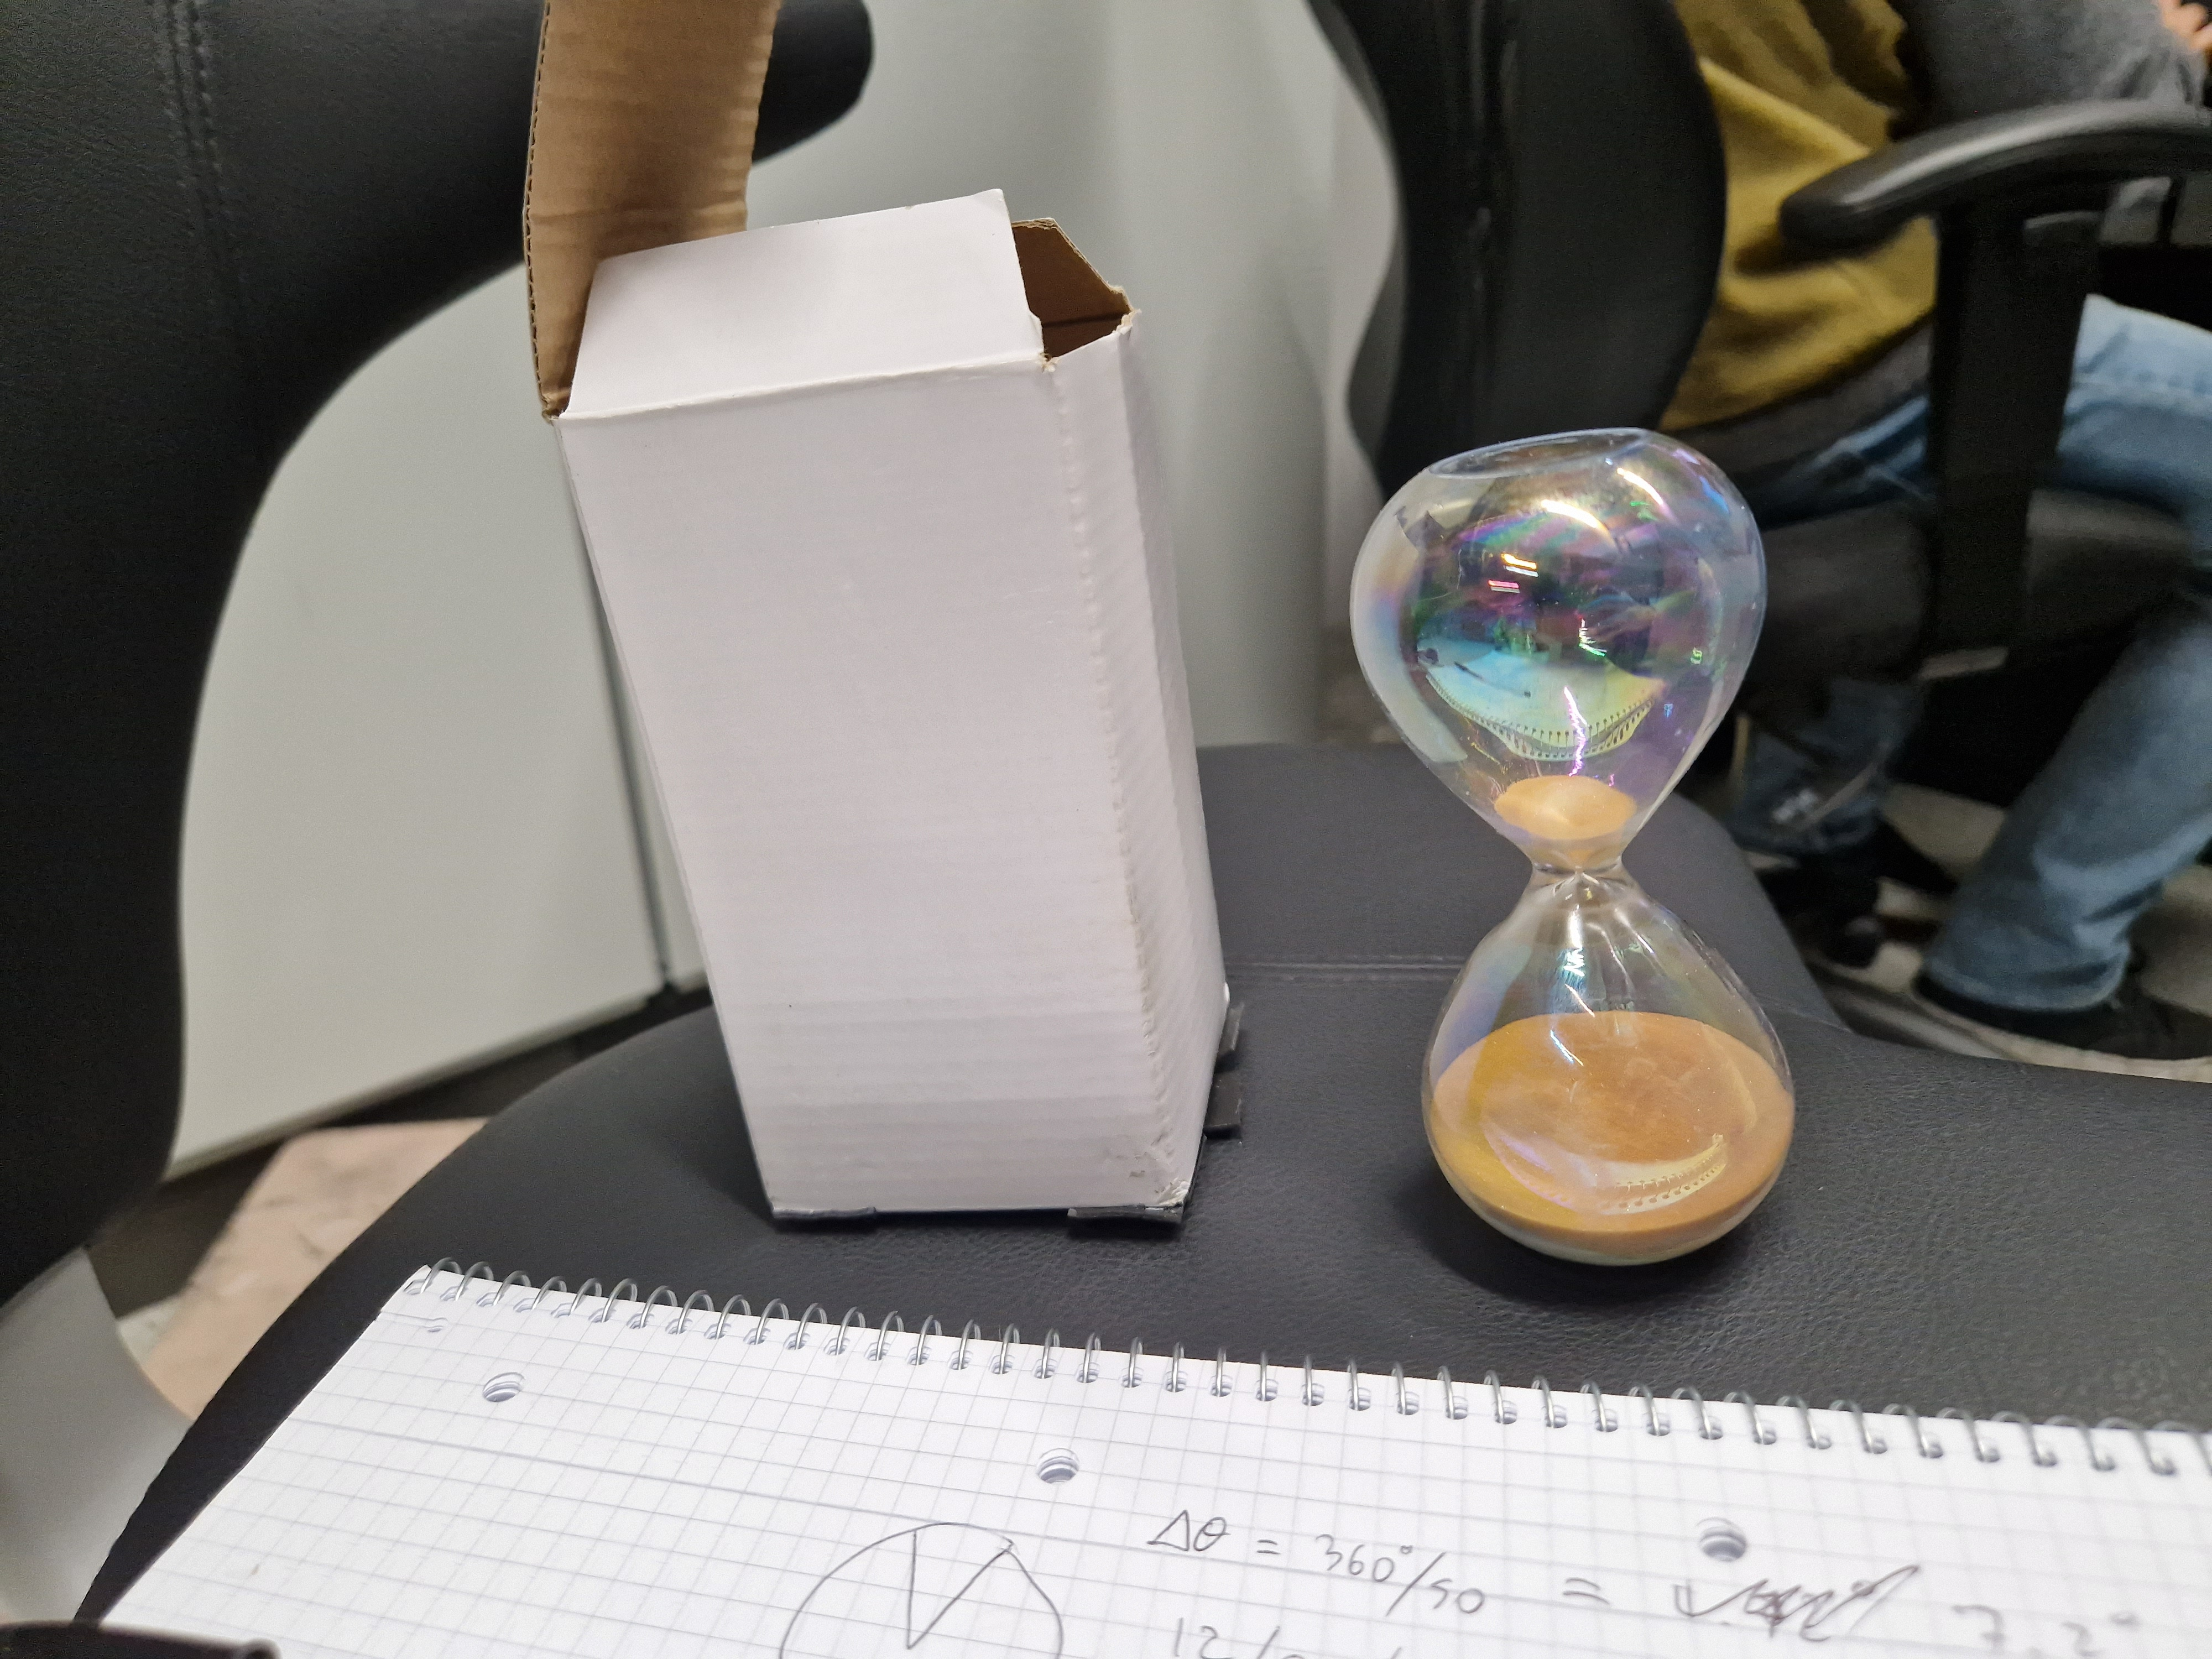
\includegraphics[width=0.85\textwidth]{hourglassandbox.jpg}
    \caption{The hourglass sample next to the enclosure used for mounting in the scanner.}
    \label{fig:hourglass}
\end{figure}

\begin{figure}[htbp]
    \centering
    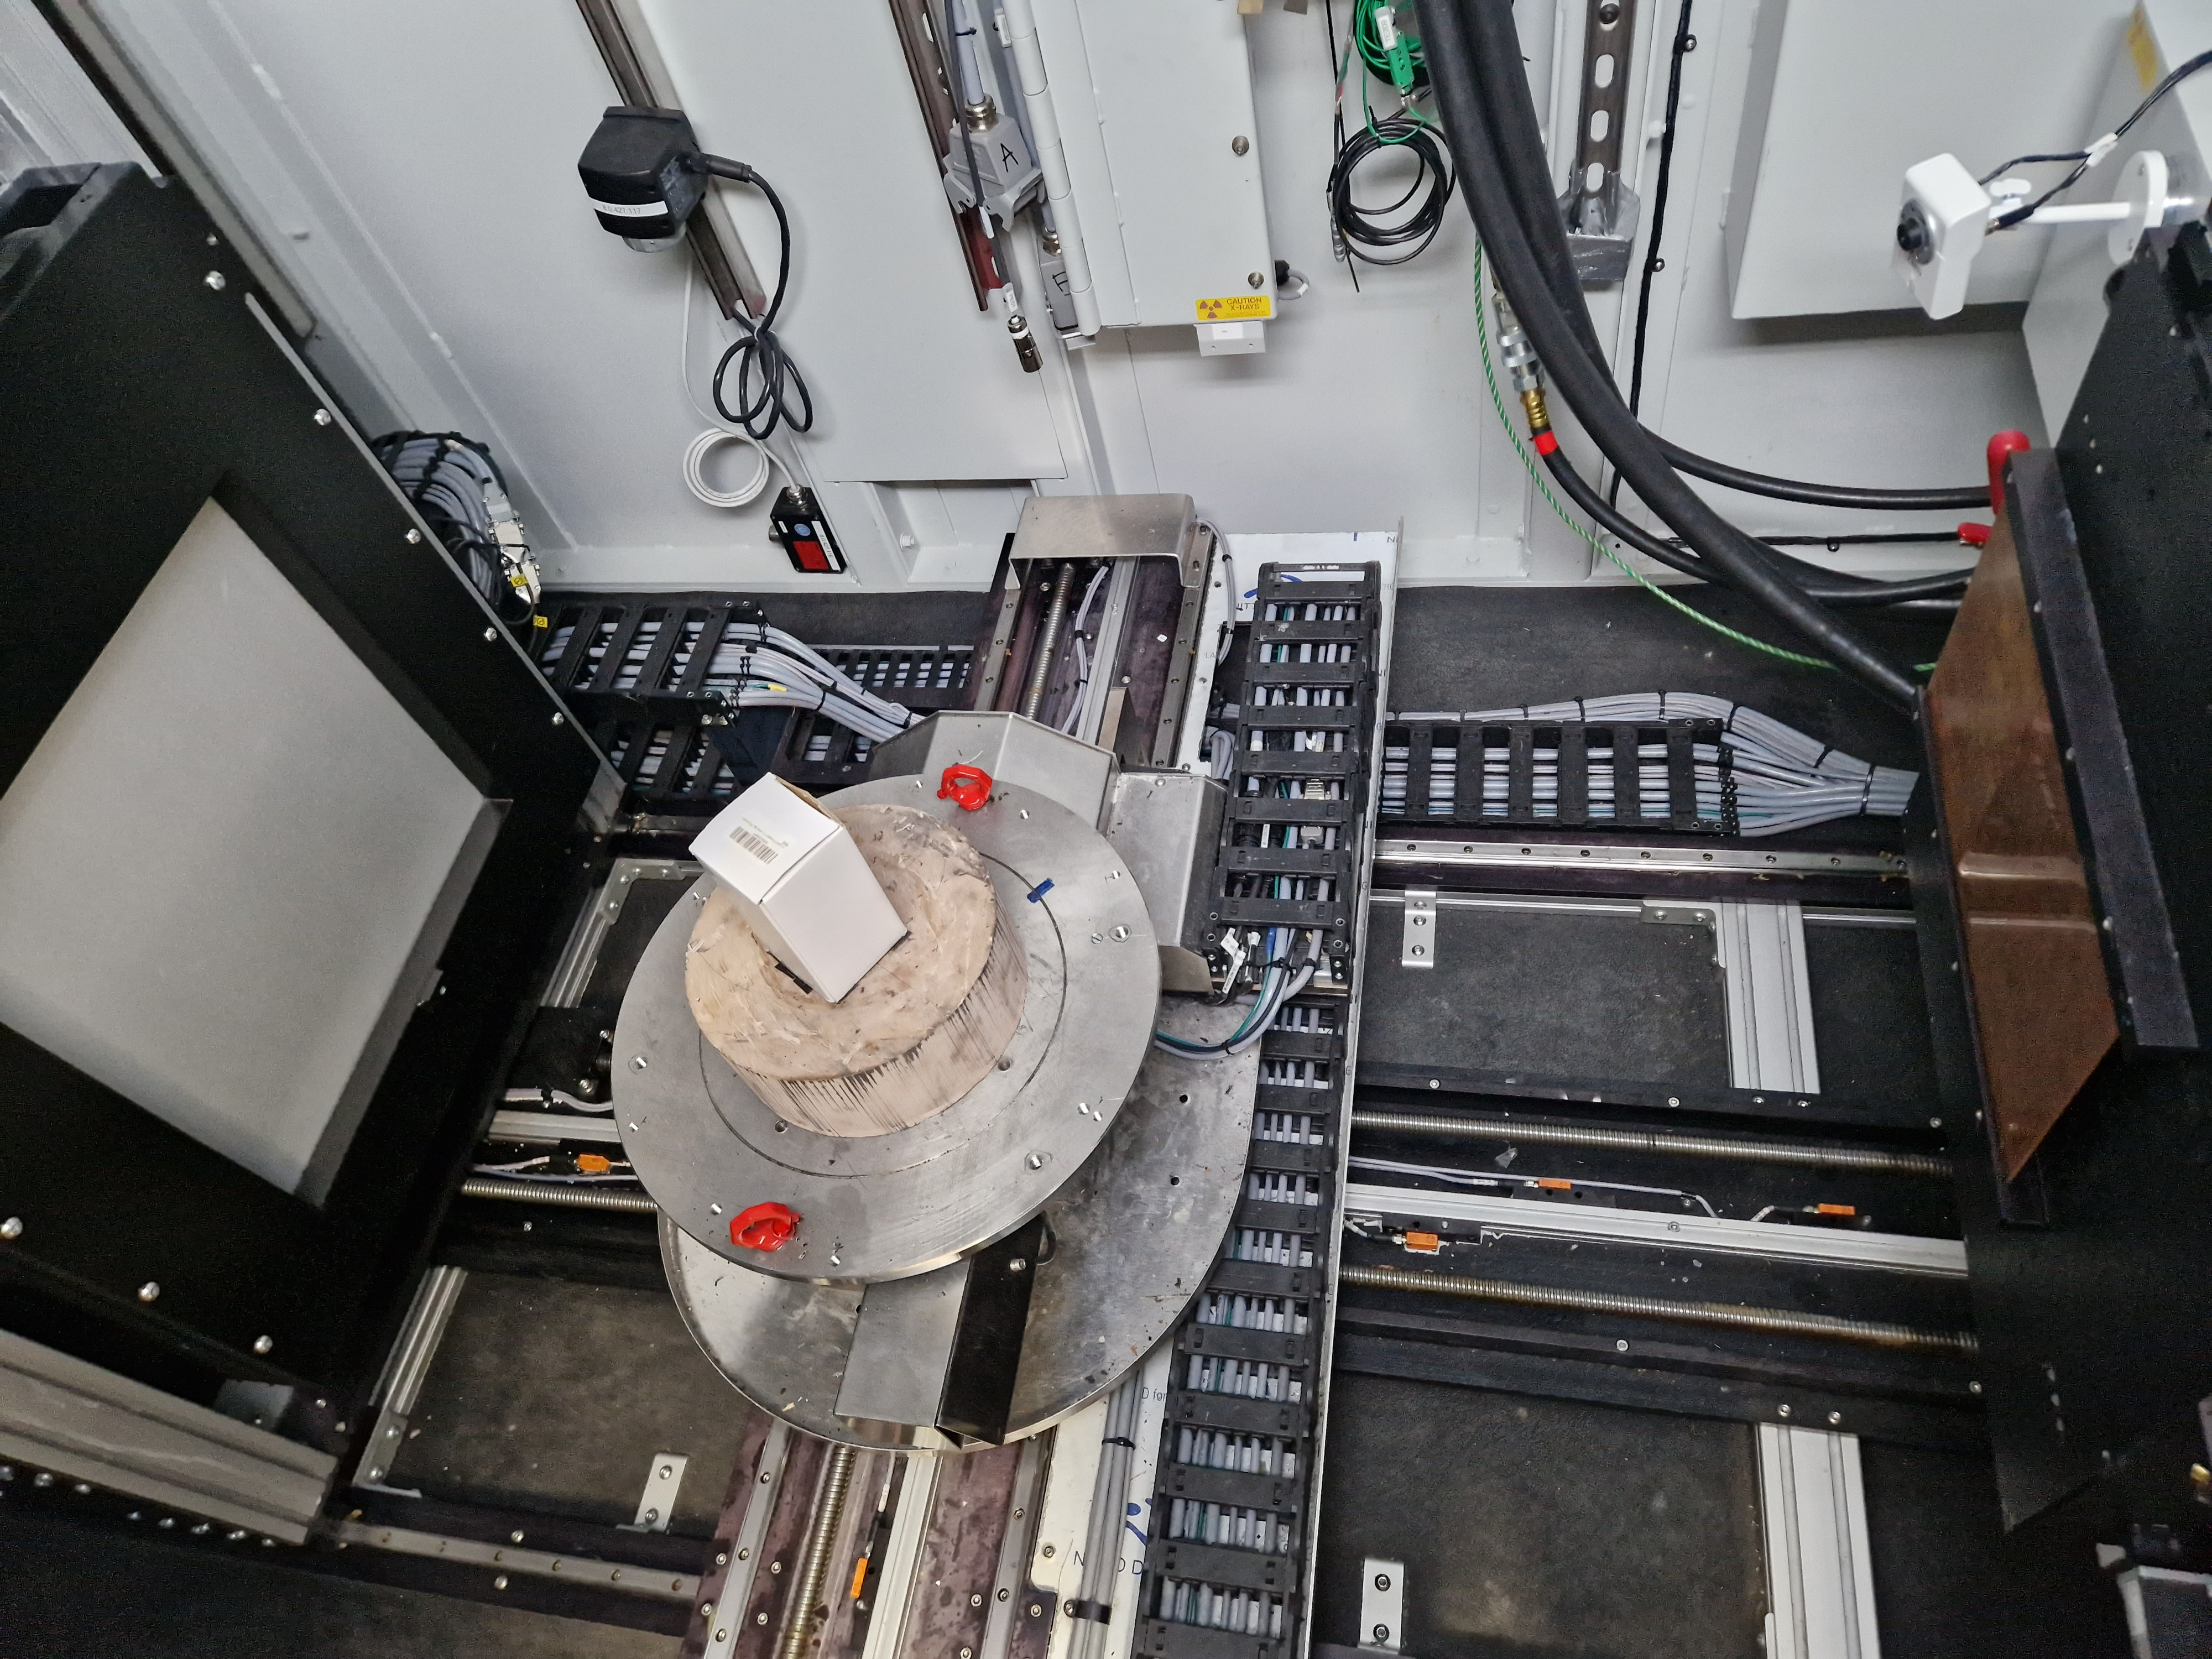
\includegraphics[width=1.0\textwidth]{hg_in_ct.jpg}
    \caption{The hourglass mounted in its enclosure inside the micro-CT scanner. To the left is the X-ray source (white), the sample sits in the centre on a rotating base, and to the right is the attenuating copper plate used as a beam stop.}
    \label{fig:hourglass_in_scanner}
\end{figure}

Six datasets were acquired, all using 800 projections in continuous rotation mode. The datasets are organised as a $3 \times 2$ factorial design, with three total angular ranges (2750\degree, 5500\degree, and 11000\degree) crossed with two frame rates (2 and 4 fps). The angular range determines the angular step per projection $\Delta\phi$, while the frame rate determines the time between consecutive projections $\Delta t$. Table~\ref{tab:acquisition_params} summarises the acquisition parameters for all six datasets.

\begin{table}[h]
  \centering
  \begin{adjustwidth}{0cm}{0cm}
  \begin{tabular}{ccccccc}
  \toprule
  \textbf{\#} & \textbf{FPS} & \textbf{Projections} & \textbf{Angle range} &
  \textbf{Total time} & \textbf{$\Delta\phi$} & \textbf{$\Delta t$} \\
  \midrule
  1 & 4 & 800 & 2750\degree  & 261\,s & 3.44\degree  & 0.44\,s \\
  2 & 4 & 800 & 5500\degree  & 233\,s & 6.88\degree  & 0.29\,s \\
  3 & 4 & 800 & 11000\degree & 223\,s & 13.75\degree & 0.28\,s \\
  4 & 2 & 800 & 2750\degree  & 417\,s & 3.44\degree  & 0.52\,s \\
  5 & 2 & 800 & 5500\degree  & 417\,s & 6.88\degree  & 0.52\,s \\
  6 & 2 & 800 & 11000\degree & 421\,s & 13.75\degree & 0.53\,s \\
  \bottomrule
  \end{tabular}
  \end{adjustwidth}
  \caption{Acquisition protocol parameters for the hourglass dynamic datasets. $\Delta\phi$ is the angular step per projection and $\Delta t$ is the time between consecutive projections.}
  \label{tab:acquisition_params}
\end{table}

The angular step $\Delta\phi$ ranges from $3.44\degree$ (datasets 1 and 4) to $13.75\degree$ (datasets 3 and 6). At the largest angular step, angular blurring from the standard $K = 1$ forward model is expected to be most severe. Datasets with the same $\Delta\phi$ but different frame rates (e.g.\ datasets 1 and 4) have the same angular blur per projection but different temporal sampling, allowing the effect of temporal resolution to be separated from the effect of angular blur.

Each dataset was reconstructed with accumulation steps $K \in \{1, 2, 3, 4, 6\}$, giving five reconstructions per dataset and thirty reconstructions in total. Table~\ref{tab:dynamic_cont_configs} lists the effective angular sub-step $\Delta\phi / K$ for each combination and highlights matched sub-step values across datasets.

\begin{table}[h]
    \centering
    \caption{Effective angular sub-step $\Delta\phi / K$ (degrees) for all combinations of dataset and accumulation steps $K$. Colour-coded entries share the same effective sub-step across different datasets, enabling controlled matched-pair comparisons. Red: 3.44\degree\ (appears in all three rows); blue: 6.88\degree; green: 1.72\degree; orange: 1.15\degree.}
    \label{tab:dynamic_cont_configs}
    \begin{tabular}{cccccc}
        \toprule
        & \multicolumn{5}{c}{Accumulation steps $K$} \\
        \cmidrule(lr){2-6}
        $\Delta\phi$ & 1 & 2 & 3 & 4 & 6 \\
        \midrule
        3.44\degree  & \textcolor{matchred}{3.44}   & \textcolor{matchgreen}{1.72}   & \textcolor{matchorange}{1.15}  & 0.86 & 0.57 \\
        6.88\degree  & \textcolor{matchblue}{6.88}   & \textcolor{matchred}{3.44}     & 2.29 & \textcolor{matchgreen}{1.72}   & \textcolor{matchorange}{1.15}  \\
        13.75\degree & 13.75 & \textcolor{matchblue}{6.88}   & 4.58 & \textcolor{matchred}{3.44}     & 2.29 \\
        \bottomrule
    \end{tabular}
\end{table}

The colour-coded entries in Table~\ref{tab:dynamic_cont_configs} identify matched pairs that allow a direct test of whether the $K$-step approximation fully recovers the quality of a finer native angular step. For example, dataset 2 ($\Delta\phi = 6.88\degree$) at $K = 2$ has the same effective sub-step of $3.44\degree$ as dataset 1 ($\Delta\phi = 3.44\degree$) at $K = 1$. If the approximation is perfect, these two should yield equal reconstruction quality.

No voxel-level ground truth is available for the hourglass dataset, because the sample is continuously evolving and a simultaneous reference acquisition is not possible. Reconstruction quality is therefore evaluated using a physically grounded volume metric. At each reconstructed time step, the volume of sand present in the upper and lower chambers is computed by segmenting the attenuation field and integrating the high-attenuation region within each chamber. Because the hourglass is a closed system with a fixed total quantity of sand, the sum of the upper and lower chamber volumes must be constant, and the rate of transfer between chambers is determined by the orifice geometry and gravity. The reconstructed volume time series is compared against this known physical trajectory, with the deviation between the reconstructed and expected chamber volumes serving as the primary quality measure. A reconstruction that faithfully captures the sand dynamics will track the monotonic depletion of the upper chamber and the corresponding filling of the lower chamber. Errors in the forward model or insufficient angular sampling will produce reconstructions where the apparent sand volume is inconsistent with the physical constraint, either failing to track the correct rate of change or introducing spurious fluctuations.

\subsection{Results}
\label{subsec:cont_dynamic_results}

\begin{figure}[htbp]
    \begin{adjustwidth}{-2cm}{-2cm}
    \centering
    \begin{subfigure}[b]{0.35\textwidth}
        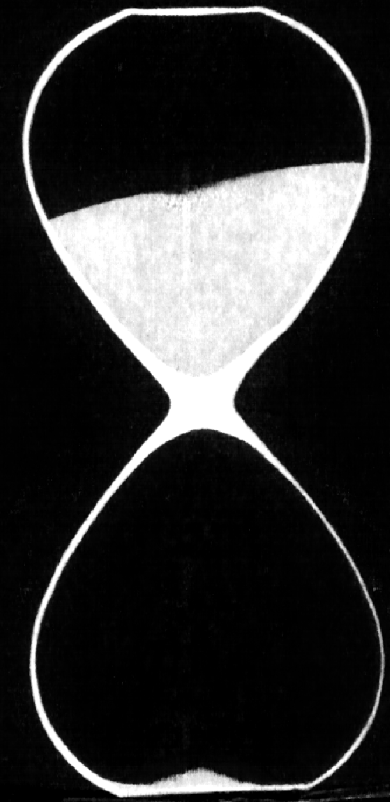
\includegraphics[width=\textwidth]{hg_con_t0.png}
        \caption{First timestep}
    \end{subfigure}
    \hspace{-0.2cm}
    \begin{subfigure}[b]{0.35\textwidth}
        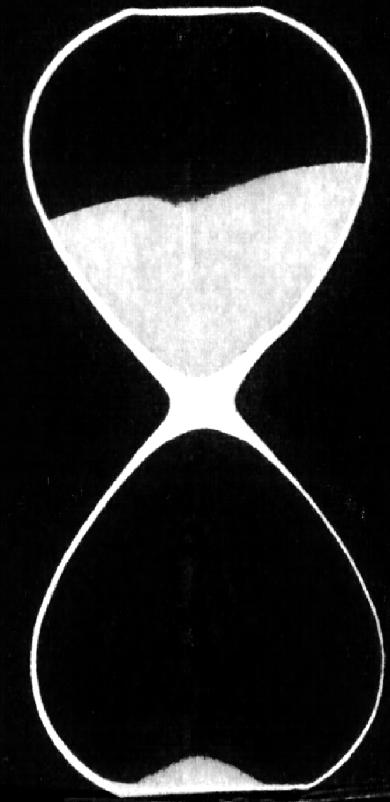
\includegraphics[width=\textwidth]{hg_con_t1.png}
        \caption{Middle timestep}
    \end{subfigure}
    \hspace{-0.2cm}
    \begin{subfigure}[b]{0.35\textwidth}
        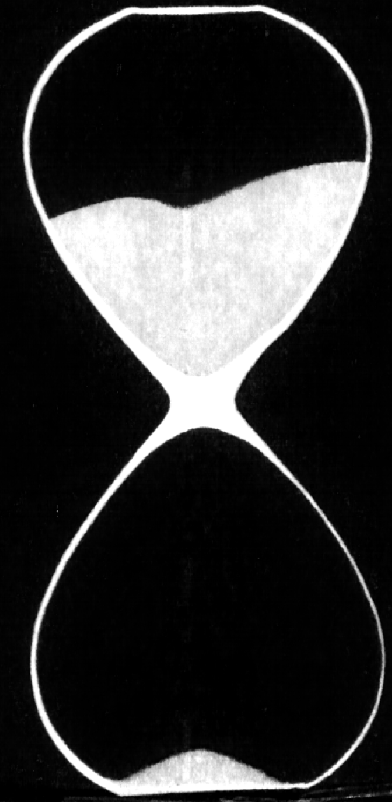
\includegraphics[width=\textwidth]{hg_con_t2.png}
        \caption{Last timestep}
    \end{subfigure}
    \end{adjustwidth}
    \caption{Dynamic reconstruction of the hourglass from dataset 1 ($\Delta\phi = 3.44\degree$, 4\,fps) at 150 epochs, shown at three time points. The redistribution of sand between the two chambers is clearly visible.}
    \label{fig:dynamic_cont_reconstruction}
\end{figure}

Figure~\ref{fig:dynamic_cont_reconstruction} shows the reconstructed hourglass at three time points from dataset 1, demonstrating that the forward model produces coherent 4D reconstructions that track the sand redistribution between chambers over time.

Figures~\ref{fig:mae_4fps} and \ref{fig:mae_2fps} show the MAE of the reconstructed sand volume trajectory for all datasets at 4\,fps and 2\,fps respectively, plotted as a function of $K$. Figure~\ref{fig:subangle_result} aggregates all thirty reconstructions on a single axis of effective sub-step size versus MAE.

\begin{figure}[htbp]
    \begin{adjustwidth}{-2cm}{0cm}
    \centering
    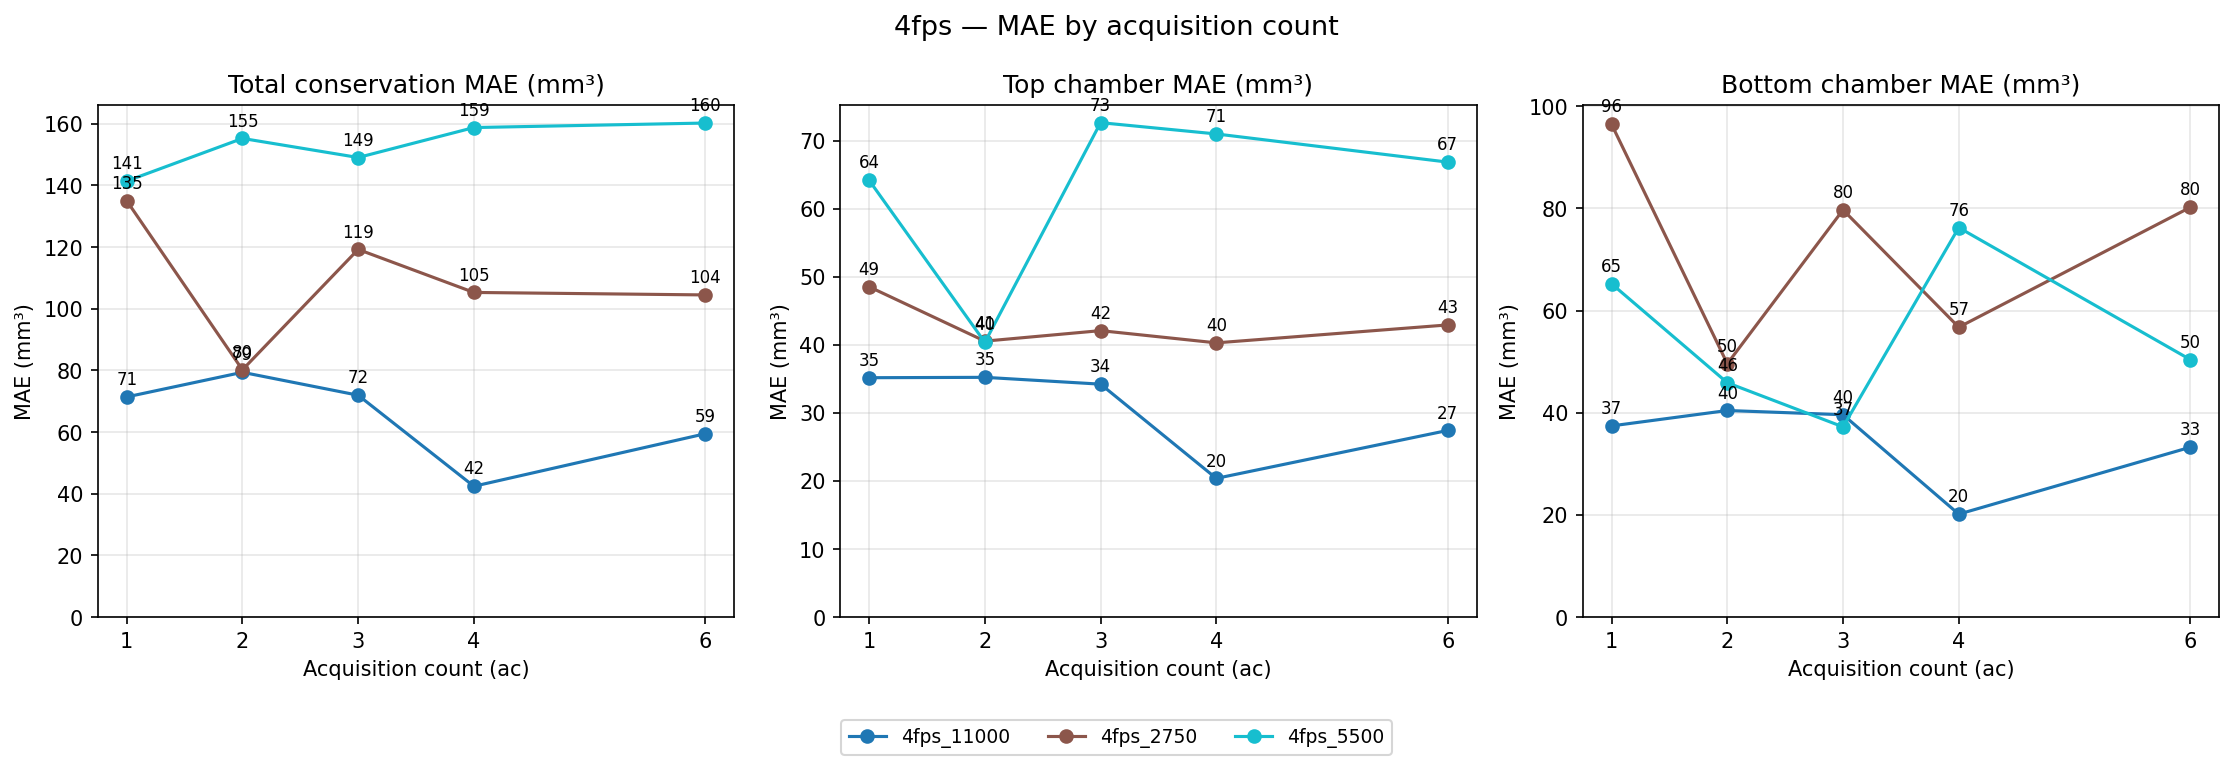
\includegraphics[width=1.2\textwidth]{continous_fail/mae_4fps.png}
    \end{adjustwidth}
    \caption{Volume MAE for the three 4\,fps datasets ($\Delta\phi = 3.44\degree$, $6.88\degree$, $13.75\degree$) as a function of accumulation steps $K$. No consistent trend is visible across $K$ values or angular step sizes.}
    \label{fig:mae_4fps}
\end{figure}

\begin{figure}[htbp]
    \begin{adjustwidth}{-2cm}{0cm}
    \centering
    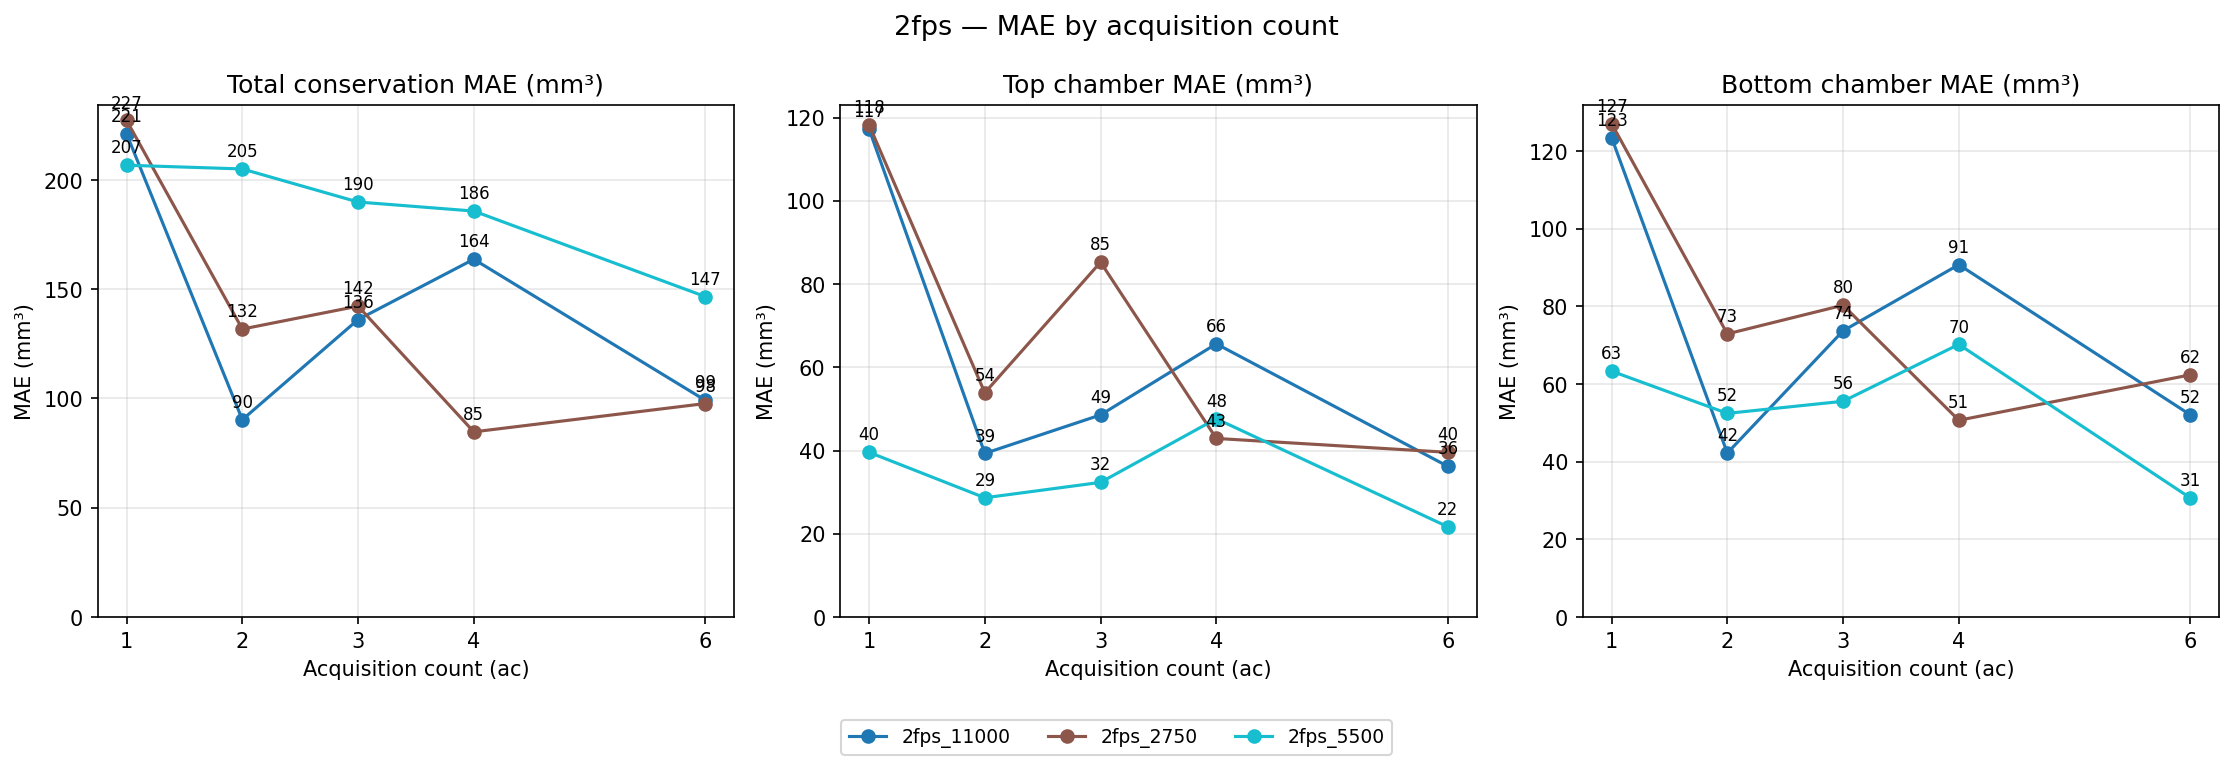
\includegraphics[width=1.2\textwidth]{continous_fail/mae_8fps.png}
    \end{adjustwidth}
    \caption{Volume MAE for the three 2\,fps datasets ($\Delta\phi = 3.44\degree$, $6.88\degree$, $13.75\degree$) as a function of accumulation steps $K$. As with the 4\,fps datasets, no correlation is observed between $K$ and reconstruction quality.}
    \label{fig:mae_2fps}
\end{figure}

\begin{figure}[H]
    \begin{adjustwidth}{-2cm}{0cm}
    \centering
    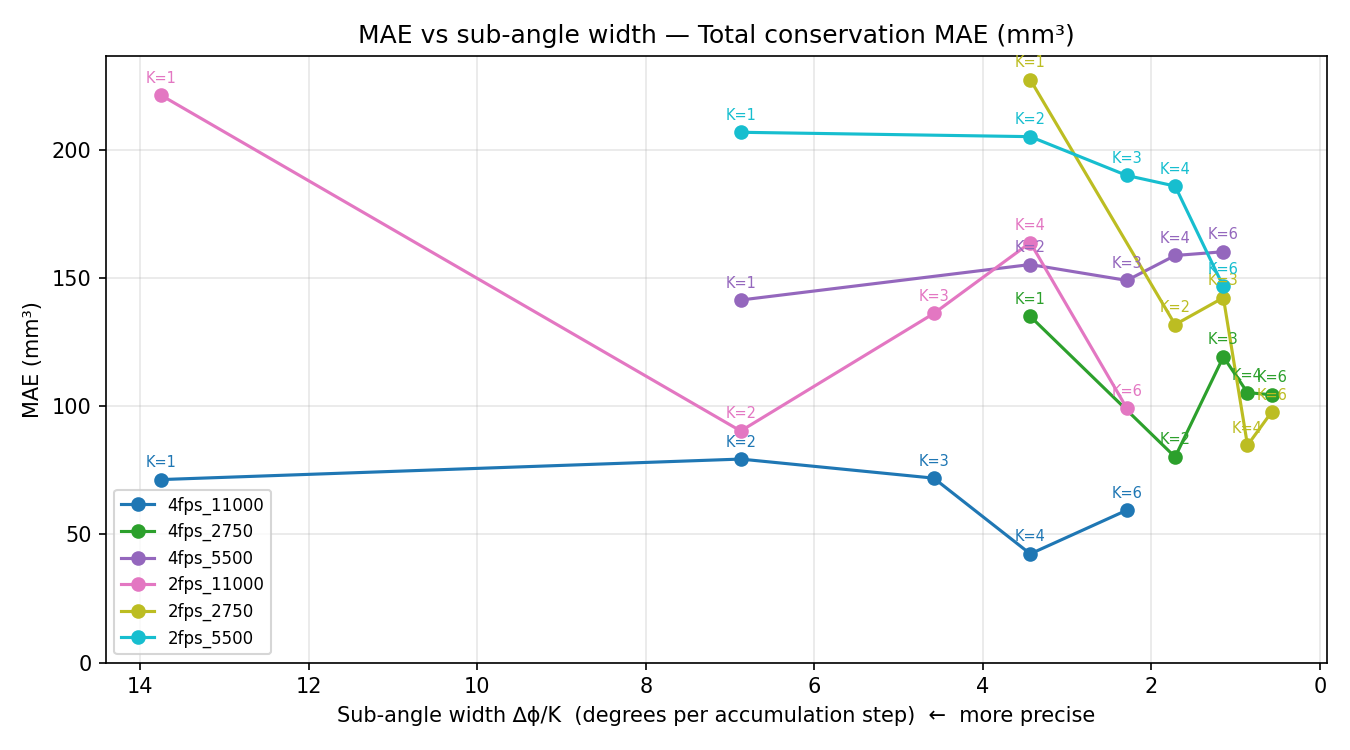
\includegraphics[width=1.2\textwidth]{continous_fail/subangle_vs_mae_total.png}
    \end{adjustwidth}
    \caption{Volume MAE for all thirty reconstructions plotted against effective sub-step size $\Delta\phi / K$. No correlation is observed across angular step sizes, frame rates, or accumulation steps, indicating that the $K$-step correction does not affect reconstruction quality for the hourglass dataset.}
    \label{fig:subangle_result}
\end{figure}

The results show no correlation between accumulation steps, angular step size, frame rate, and reconstruction quality. Increasing $K$ from 1 to 6 produces no consistent improvement in volume MAE for any of the six datasets, and the matched-pair comparisons across different angular steps yield no evidence that a higher $K$ compensates for a larger $\Delta\phi$.


% ─────────────────────────────────────────────────────────────────────────────
\section{Discussion}
\label{sec:cont_discussion}
% ─────────────────────────────────────────────────────────────────────────────

\subsection{Requirements for the Continuous-Scan Forward Model}
\label{subsec:cont_disc_requirements}

Taken together, the static and dynamic experiments allow a clear statement of what is needed for the $K$-step continuous-scan forward model to produce genuine improvement in reconstruction quality. Three conditions must be satisfied simultaneously.

The first requirement is that the sample must have directional angular structure. The projection data must carry meaningfully different structural information from different viewing angles. For angularly isotropic samples, projections at nearby angles are essentially equivalent, angular blur does not degrade the information content of each projection, and the correction has nothing to recover. The Bentheimer sandstone satisfies this requirement. The hourglass does not.

The second requirement is that the acquisition must span multiple revolutions following a space-filling angular scheme such as the hybrid golden-section pattern. A single revolution cannot enable sub-angle decoupling because consecutive projections are angularly adjacent and their sub-angles do not create cross-projection constraints. Any gain from increasing $K$ with a single revolution reflects numerical quadrature improvement rather than genuine sub-angle resolution. Multiple revolutions progressively place sub-angles from later projections into the gaps left by earlier ones, building a dense and mutually constrained angular coverage that allows the model to separate individual sub-angle contributions. The hourglass experiment spans multiple revolutions and satisfies this requirement. The static Bentheimer acquisition does not.

The third requirement is that the angular step size per projection must be large enough for blur to be a meaningful source of reconstruction error. For small $\Delta\phi$, the step-and-shoot forward model at $K = 1$ already approximates the true angular integral well, and increasing $K$ provides diminishing returns. The benefit of the correction is greatest when $\Delta\phi$ is large and the single-midpoint approximation introduces substantial geometric error.

The static Bentheimer experiment satisfies requirements one and three but not two. The hourglass experiment satisfies requirements two and three but not one. Neither dataset simultaneously satisfies all three conditions. The Bentheimer result shows that angular blur correction is valid and implementable, but is capped by single-revolution degeneracy. The hourglass result shows that multi-revolution acquisition is achievable and does not introduce new failure modes, but the angular isotropy of the sample makes the correction irrelevant.

\subsection{Sample Geometry and the Hourglass Result}
\label{subsec:cont_disc_dynamic}

The absence of any correlation between $K$, $\Delta\phi$, frame rate, and reconstruction quality in the hourglass experiment is explained by the cylindrical symmetry of the sample. Sand is a dense granular medium with near-circular cross-section, and the two-chamber geometry is symmetric around the rotation axis. A projection at any angle carries essentially the same structural information as a projection at a nearby angle. Even when sub-angles from multiple revolutions create overlapping constraints, the signal variation between those angles is negligible, so the additional equations add no useful information. The model reconstructs the sand volume accurately regardless of $K$ because the projections are uniformly informative at all angles.

This is a distinct failure from the static experiment. In the static case the sample has angular structure but the acquisition design prevents decoupling. In the hourglass case the acquisition design supports decoupling but the sample provides nothing to decouple. Both lead to the same outcome of negligible improvement from increasing $K$, but for fundamentally different reasons.

Two implementation assumptions are also worth noting for future extensions. The current model assumes constant angular velocity and computes per-projection angular intervals from a single global value. Accepting per-projection intervals as input would broaden applicability to instruments with variable rotation speed or alternating-direction acquisition. The model also assumes the attenuation field is static within each projection's exposure interval, which holds for the hourglass at the frame rates used but would break down for faster dynamic processes where intra-exposure sample motion is non-negligible.


% ═════════════════════════════════════════════════════════════════════════════
\chapter{Conclusion}
\label{chap:conclusion}
% ═════════════════════════════════════════════════════════════════════════════

The original NeCT implementation required approximately 45\,GB of GPU memory and over 40 hours of training per dataset, restricting the method to a handful of research-grade GPUs and making it impractical for any workflow requiring rapid turnaround. \NeCTv{} changes that. By identifying and correcting a fundamental structural inefficiency in the QuadCubes encoder design, namely the over-provisioning of the temporal encoders relative to the spatial encoder, two new architectures are introduced that outperform the original on every metric simultaneously. \CombinedCubes{} achieves this by replacing the large 3D temporal hash encoders with collision-free 2D encoders, and \MixedCubes{}\footnote{All architectures are publicly available at \url{https://github.com/kristiancarlenius/NeCTv2}.} goes further with fully dense temporal grids that guarantee an exact coordinate-to-feature correspondence. The best \MixedCubes{} configuration reaches 37.73\,dB PSNR in 24 hours at 22.1\,GB, a gain of 1.84\,dB over the QuadCubes baseline at roughly half the memory and in substantially less wall-clock time per epoch. A lightweight variant matches baseline quality at 5.1\,GB, bringing NeCT-class 4D-CT reconstruction within reach of any CUDA-capable GPU for the first time. For practitioners already using NeCT, switching to \MixedCubes{} is a strict improvement at every hardware tier: higher quality, lower memory, and no sacrifice in reconstruction fidelity.

The second part of this thesis extended the NeCT forward model to continuous-rotation scanning, deriving a $K$-step midpoint approximation of the angular averaging integral that arises when the sample rotates during each exposure. Two implementations are provided, one optimised for speed and one for memory, with the memory-efficient mode making the accumulation step count a free parameter independent of GPU capacity. The validation experiments confirmed that the correction is implemented correctly and recovers quality lost to angular blur. They also made clear that the method's full benefit depends on three conditions being met at once. The sample must have directional angular structure so that different projection angles carry genuinely different information. The acquisition must span multiple golden-angle revolutions so that sub-angles from later projections overlap with earlier ones and the model can decouple their contributions. And the per-projection angular step must be large enough for angular blur to be a real source of error. Neither the single-revolution Bentheimer dataset nor the angularly isotropic hourglass met all three of these at once, which is why neither showed the full improvement the theory predicts. The forward model is correct. What remains is the right dataset to test it on.

\section{Further Work}
\label{sec:conclusion_future}

The most direct and important open experiment is to acquire or generate a dataset that satisfies all three conditions identified above, and to evaluate the $K$-step continuous-scan forward model on it. A sample with fine directional structure, such as a rock undergoing anisotropic fracture propagation or a layered material experiencing differential dissolution, acquired over multiple golden-angle revolutions with a per-projection angular step large enough to produce visible blur at $K = 1$, would allow a definitive test of whether continuous-scan reconstruction genuinely improves on step-and-shoot reconstruction at the same projection count. Until such a dataset is tested, the potential benefit of the continuous-scan forward model remains theoretically grounded but empirically unconfirmed.

Beyond this primary experiment, several extensions are worth pursuing. The encoder optimisation results were obtained on a single dataset, and while the governing design principles have theoretical grounding in hash collision rates and encoder dimensionality, the specific optimal configurations may shift for datasets with different pore geometry, faster dynamics, or different spatial-to-temporal signal ratios. Testing whether the \MixedCubes{} recommendations transfer to other sample types is an important step toward general deployment of \NeCTv{}. The forward model currently assumes constant angular velocity and computes angular intervals from a single global rotation speed. Accepting per-projection intervals as input would broaden applicability to instruments with variable rotation or alternating-direction scanning without any change to the core model. Finally, reconstruction time remains on the order of hours on a single GPU, and reducing this further through multi-GPU data-parallel training or better initialisation strategies would make the method more practical for workflows requiring rapid turnaround.

% ─── Code Availability ──────────────────────────────────────────────────────
\section*{Code Availability}
\addcontentsline{toc}{section}{Code Availability}

The full source code for \NeCTv{}, including all encoder architectures (\QuadCubes, \CombinedCubes, and \MixedCubes{}) and the continuous-scan forward model, is publicly available at \url{https://github.com/kristiancarlenius/NeCTv2}.

% ─── Bibliography ────────────────────────────────────────────────────────────
\cleardoublepage
\bibliographystyle{plainnat}
\bibliography{references}

% ─── Appendices ──────────────────────────────────────────────────────────────
\appendix

\chapter{Complete Experimental Results}
\label{app:experimental}

This appendix reports PSNR reconstruction quality for all configurations evaluated in Part~\ref{part:encoder_optimisation}. Table~\ref{tab:app_time} gives PSNR at each 6-hour wall-clock checkpoint, Table~\ref{tab:app_epoch} gives PSNR at each 50-epoch checkpoint, Table~\ref{tab:app_summary} gives a full summary of all three metrics at epoch~500 and at the final timed snapshot. Dashes indicate that a configuration did not reach that time or epoch budget. The QuadCubes baseline (\texttt{23\_4\_23\_4\_128}, 44.8\,GB) is marked with $\dagger$.

% ── Table 1: PSNR by wall-clock time ─────────────────────────────────────────

\begin{table}[htbp]
\caption{PSNR (dB) at each 6-hour wall-clock checkpoint for all evaluated configurations. Dashes indicate the training run did not reach that wall-clock time.}
\label{tab:app_time}
\begin{adjustwidth}{-3cm}{-1cm}
\centering
\footnotesize
\setlength{\tabcolsep}{4pt}
\begin{tabular}{llrrrrrrrr}
\toprule
Architecture & Config & VRAM & \multicolumn{7}{c}{PSNR at wall-clock time (h)} \\
\cmidrule(lr){4-10}
 & & (GB) & 0 & 6 & 12 & 18 & 24 & 30 & 36 \\
\midrule
  QuadCubes & \texttt{23\_4\_21\_4\_128} &   & 33.37 & 34.45 & 35.02 & 35.26 &   &   &   \\
   & \texttt{23\_4\_17\_4\_128} & 1.4 & 30.25 & 30.68 & 30.81 &   &   &   &   \\
   & \texttt{23\_4\_18\_4\_128} & 2.3 & 31.21 & 31.75 & 31.88 &   &   &   &   \\
   & \texttt{23\_4\_19\_4\_128} & 4.0 & 31.77 & 32.64 & 32.99 & 33.00 &   &   &   \\
   & \texttt{23\_4\_20\_4\_128} & 7.1 & 32.65 & 33.59 & 34.03 & 34.13 &   &   &   \\
   & \texttt{23\_1\_23\_4\_128} & 11.5 & 32.76 & 33.79 & 34.27 & 34.40 &   &   &   \\
   & \texttt{21\_4\_21\_4\_128} & 11.9 & 33.31 & 34.45 & 34.96 & 35.04 &   &   &   \\
   & \texttt{23\_2\_23\_4\_128} & 22.6 & 33.57 & 34.84 & 35.43 & 35.84 & 36.00 &   &   \\
   & \texttt{22\_4\_22\_4\_128} & 23.1 & 33.45 & 34.84 & 35.44 & 35.87 & 36.06 &   &   \\
   & \texttt{23\_4\_22\_4\_128} & 24.1 & 33.38 & 34.70 & 35.34 & 35.77 & 35.98 & 36.02 &   \\
   & \texttt{17\_4\_23\_4\_128} & 33.0 & 33.41 & 34.97 & 35.65 & 36.08 & 36.32 & 36.35 &   \\
   & \texttt{18\_4\_23\_4\_128} & 35.2 & 33.53 & 35.14 & 35.84 & 36.29 & 36.55 & 36.63 &   \\
   & \texttt{19\_4\_23\_4\_128} & 36.9 & 33.26 & 34.89 & 35.62 & 36.07 & 36.33 & 36.44 &   \\
   & \texttt{20\_4\_23\_4\_128} & 39.0 & 33.25 & 34.94 & 35.55 & 36.07 & 36.35 & 36.48 &   \\
   & \texttt{21\_4\_23\_4\_128} & 40.8 & 32.95 & 34.75 & 35.44 & 35.93 & 36.27 & 36.41 & 36.45 \\
   & \texttt{22\_4\_23\_4\_128} & 42.8 & 32.73 & 34.65 & 35.37 & 35.90 & 36.23 & 36.45 & 36.52 \\
   & \texttt{23\_4\_23\_4\_128}$^\dagger$ & 44.8 & 33.07 & 34.86 & 35.50 & 35.89 & 36.14 & 36.33 & 36.45 \\
\addlinespace
  Sp.~heavy & \texttt{23\_4\_23\_4\_128} & 20.1 & 34.47 & 35.64 & 36.27 & 36.60 &   &   &   \\
   & \texttt{24\_4\_24\_4\_128} & 24.1 & 34.60 & 36.16 & 36.96 & 37.53 & 37.85 &   &   \\
\addlinespace
  Temp.~heavy & \texttt{19\_4\_19\_4\_128} & 34.4 & 30.45 & 31.21 & 31.54 & 31.68 & 31.76 & 31.78 &   \\
   & \texttt{21\_4\_21\_4\_128} & 36.5 & 32.26 & 33.45 & 34.05 & 34.46 & 34.69 & 34.78 &   \\
\addlinespace
  CombinedCubes & \texttt{22\_4\_22\_4\_128} & 8.0 & 33.27 & 34.93 & 35.82 & 36.36 & 36.55 &   &   \\
   & \texttt{22\_4\_22\_6\_128} & 8.3 & 33.21 & 34.83 & 35.66 & 36.24 & 36.46 &   &   \\
   & \texttt{18\_4\_23\_6\_64} & 10.9 & 33.47 & 35.03 & 35.94 & 36.49 & 36.67 &   &   \\
   & \texttt{23\_4\_23\_4\_128} & 13.8 & 32.88 & 34.70 & 35.59 & 36.21 & 36.61 &   &   \\
   & \texttt{18\_4\_24\_4\_128} & 18.3 & 34.04 & 35.69 & 36.63 & 37.28 & 37.54 &   &   \\
   & \texttt{18\_2\_24\_4\_128} & 19.5 & 32.70 & 34.44 & 35.07 & 35.38 & 35.58 & 35.77 &   \\
   & \texttt{22\_4\_24\_6\_64} & 22.4 & 33.08 & 34.87 & 35.87 & 36.54 & 37.02 &   &   \\
   & \texttt{24\_4\_24\_6\_128} & 24.3 & 32.88 & 35.08 & 36.29 & 37.18 & 37.97 &   &   \\
   & \texttt{16\_4\_25\_4\_128} & 28.6 & 33.70 & 35.48 & 36.36 & 37.02 & 37.44 & 37.60 &   \\
   & \texttt{19\_4\_25\_4\_128} & 34.0 & 33.32 & 35.24 & 36.06 & 36.66 & 37.18 & 37.49 & 37.60 \\
   & \texttt{22\_4\_25\_4\_128} & 39.0 & 33.08 & 35.02 & 35.96 & 36.64 & 37.12 &   &   \\
\addlinespace
  \MixedCubes{} & \texttt{18\_4\_22\_4\_64} & 5.1 & 34.25 & 35.38 & 35.94 & 35.97 &   &   &   \\
   & \texttt{18\_4\_23\_6\_128} & 9.1 & 34.53 & 35.74 & 36.53 & 36.81 &   &   &   \\
   & \texttt{20\_2\_24\_4\_128} & 10.8 & 33.93 & 35.31 & 36.03 & 36.57 & 36.75 &   &   \\
   & \texttt{23\_4\_23\_4\_128} & 13.1 & 34.70 & 35.85 & 36.59 & 36.88 &   &   &   \\
   & \texttt{18\_4\_24\_4\_128} & 16.7 & 34.76 & 36.08 & 36.79 & 37.31 &   &   &   \\
   & \texttt{24\_4\_24\_4\_128} & 22.1 & 34.45 & 36.07 & 36.97 & 37.73 & 38.16 & 38.25 &   \\
   & \texttt{25\_2\_25\_4\_128} & 25.5 & 32.30 & 34.13 & 34.81 & 35.37 & 35.76 & 35.98 & 36.13 \\
   & \texttt{16\_4\_25\_4\_128} & 26.9 & 34.46 & 35.72 & 36.52 & 37.06 & 37.31 &   &   \\
   & \texttt{22\_4\_22\_4\_128} & 32.1 & 33.28 & 34.59 & 35.32 & 35.82 & 36.20 & 36.35 &   \\
   & \texttt{19\_4\_25\_4\_128} & 32.1 & 34.20 & 35.60 & 36.33 & 36.87 & 37.22 & 37.34 &   \\
   & \texttt{22\_4\_25\_4\_128} & 36.9 & 34.14 & 35.41 & 36.10 & 36.70 & 37.07 & 37.28 &   \\
\addlinespace
\bottomrule
\end{tabular}
\end{adjustwidth}
\end{table}

% ── Table 2: PSNR by epoch ───────────────────────────────────────────────────

\begin{table}[htbp]
\caption{PSNR (dB) at each 50-epoch checkpoint for all evaluated configurations.}
\label{tab:app_epoch}
\begin{adjustwidth}{-3cm}{-1cm}
\centering
\footnotesize
\setlength{\tabcolsep}{3.5pt}
\begin{tabular}{llrrrrrrrrrrr}
\toprule
Architecture & Config & VRAM & \multicolumn{10}{c}{PSNR at epoch} \\
\cmidrule(lr){4-13}
 & & (GB) & 50 & 100 & 150 & 200 & 250 & 300 & 350 & 400 & 450 & 500 \\
\midrule
  QuadCubes & \texttt{23\_4\_21\_4\_128} &   & 31.28 & 33.07 & 33.77 & 34.23 & 34.55 & 34.79 & 35.02 & 35.16 & 35.25 & 35.29 \\
   & \texttt{23\_4\_17\_4\_128} & 1.4 & 29.09 & 29.84 & 30.16 & 30.35 & 30.48 & 30.61 & 30.69 & 30.74 & 30.79 & 30.81 \\
   & \texttt{23\_4\_18\_4\_128} & 2.3 & 29.70 & 30.69 & 31.07 & 31.28 & 31.45 & 31.59 & 31.71 & 31.79 & 31.85 & 31.87 \\
   & \texttt{23\_4\_19\_4\_128} & 4.0 & 30.08 & 31.37 & 31.88 & 32.19 & 32.46 & 32.64 & 32.79 & 32.91 & 32.97 & 32.99 \\
   & \texttt{23\_4\_20\_4\_128} & 7.1 & 30.52 & 32.08 & 32.74 & 33.15 & 33.46 & 33.67 & 33.87 & 34.00 & 34.09 & 34.12 \\
   & \texttt{23\_1\_23\_4\_128} & 11.5 & 30.56 & 32.32 & 33.06 & 33.47 & 33.79 & 34.02 & 34.21 & 34.30 & 34.38 & 34.40 \\
   & \texttt{21\_4\_21\_4\_128} & 11.9 & 30.73 & 32.60 & 33.43 & 33.92 & 34.30 & 34.53 & 34.75 & 34.91 & 35.00 & 35.04 \\
   & \texttt{23\_2\_23\_4\_128} & 22.6 & 31.32 & 33.57 & 34.43 & 34.93 & 35.26 & 35.53 & 35.77 & 35.89 & 35.99 & 36.01 \\
   & \texttt{22\_4\_22\_4\_128} & 23.1 & 31.72 & 33.68 & 34.51 & 34.95 & 35.30 & 35.59 & 35.81 & 35.96 & 36.05 & 36.08 \\
   & \texttt{23\_4\_22\_4\_128} & 24.1 & 31.83 & 33.69 & 34.45 & 34.95 & 35.28 & 35.54 & 35.75 & 35.91 & 36.01 & 36.02 \\
   & \texttt{17\_4\_23\_4\_128} & 33.0 & 31.76 & 33.82 & 34.73 & 35.23 & 35.57 & 35.84 & 36.07 & 36.23 & 36.32 & 36.35 \\
   & \texttt{18\_4\_23\_4\_128} & 35.2 & 31.96 & 34.10 & 34.95 & 35.50 & 35.84 & 36.14 & 36.35 & 36.50 & 36.60 & 36.63 \\
   & \texttt{19\_4\_23\_4\_128} & 36.9 & 31.50 & 33.88 & 34.79 & 35.32 & 35.70 & 35.95 & 36.19 & 36.33 & 36.42 & 36.44 \\
   & \texttt{20\_4\_23\_4\_128} & 39.0 & 31.83 & 34.08 & 34.94 & 35.40 & 35.75 & 36.03 & 36.25 & 36.40 & 36.48 & 36.50 \\
   & \texttt{21\_4\_23\_4\_128} & 40.8 & 31.69 & 33.92 & 34.80 & 35.33 & 35.70 & 35.99 & 36.19 & 36.36 & 36.42 & 36.45 \\
   & \texttt{22\_4\_23\_4\_128} & 42.8 & 31.85 & 34.00 & 34.85 & 35.37 & 35.77 & 36.04 & 36.24 & 36.41 & 36.50 & 36.53 \\
   & \texttt{23\_4\_23\_4\_128}$^\dagger$ & 44.8 & 32.12 & 34.30 & 35.09 & 35.55 & 35.83 & 36.06 & 36.19 & 36.33 & 36.43 & 36.47 \\
\addlinespace
  Sp.~heavy & \texttt{23\_4\_23\_4\_128} & 20.1 & 32.44 & 34.25 & 34.99 & 35.49 & 35.82 & 36.12 & 36.35 & 36.52 & 36.61 & 36.65 \\
   & \texttt{24\_4\_24\_4\_128} & 24.1 & 32.89 & 35.00 & 35.84 & 36.41 & 36.83 & 37.17 & 37.49 & 37.73 & 37.85 & 37.86 \\
\addlinespace
  Temp.~heavy & \texttt{19\_4\_19\_4\_128} & 34.4 & 29.64 & 30.77 & 31.14 & 31.36 & 31.54 & 31.63 & 31.69 & 31.74 & 31.77 & 31.77 \\
   & \texttt{21\_4\_21\_4\_128} & 36.5 & 31.12 & 32.64 & 33.37 & 33.80 & 34.10 & 34.37 & 34.55 & 34.68 & 34.76 & 34.79 \\
\addlinespace
  CombinedCubes & \texttt{22\_4\_22\_4\_128} & 8.0 & 31.08 & 33.27 & 34.23 & 34.93 & 35.43 & 35.82 & 36.15 & 36.36 & 36.50 & 36.55 \\
   & \texttt{22\_4\_22\_6\_128} & 8.3 & 31.09 & 33.21 & 34.16 & 34.83 & 35.34 & 35.75 & 36.07 & 36.29 & 36.42 & 36.47 \\
   & \texttt{18\_4\_23\_6\_64} & 10.9 & 31.25 & 33.31 & 34.29 & 34.97 & 35.49 & 35.88 & 36.24 & 36.48 & 36.62 & 36.66 \\
   & \texttt{23\_4\_23\_4\_128} & 13.8 & 31.13 & 33.36 & 34.36 & 35.10 & 35.59 & 35.99 & 36.31 & 36.58 & 36.70 & 36.75 \\
   & \texttt{18\_4\_24\_4\_128} & 18.3 & 32.04 & 34.16 & 35.15 & 35.89 & 36.40 & 36.81 & 37.19 & 37.42 & 37.54 & 37.59 \\
   & \texttt{18\_2\_24\_4\_128} & 19.5 & 31.80 & 33.92 & 34.71 & 35.07 & 35.35 & 35.50 & 35.68 & 35.81 & 35.92 & 35.99 \\
   & \texttt{22\_4\_24\_6\_64} & 22.4 & 31.45 & 33.71 & 34.78 & 35.51 & 36.01 & 36.45 & 36.83 & 37.07 & 37.22 & 37.26 \\
   & \texttt{24\_4\_24\_6\_128} & 24.3 & 31.83 & 34.24 & 35.51 & 36.41 & 37.13 & 37.72 & 38.25 & 38.62 & 38.80 & 38.88 \\
   & \texttt{16\_4\_25\_4\_128} & 28.6 & 32.18 & 34.32 & 35.30 & 35.99 & 36.45 & 36.89 & 37.21 & 37.44 & 37.56 & 37.60 \\
   & \texttt{19\_4\_25\_4\_128} & 34.0 & 32.13 & 34.36 & 35.36 & 36.01 & 36.53 & 36.91 & 37.22 & 37.47 & 37.59 & 37.61 \\
   & \texttt{22\_4\_25\_4\_128} & 39.0 & 32.12 & 34.45 & 35.46 & 36.16 & 36.64 & 37.05 & 37.38 & 37.60 & 37.72 & 37.73 \\
\addlinespace
  \MixedCubes{} & \texttt{18\_4\_22\_4\_64} & 5.1 & 31.85 & 33.36 & 34.15 & 34.64 & 35.03 & 35.30 & 35.60 & 35.81 & 35.93 & 35.96 \\
   & \texttt{18\_4\_23\_6\_128} & 9.1 & 32.38 & 34.00 & 34.80 & 35.33 & 35.74 & 36.09 & 36.40 & 36.62 & 36.76 & 36.79 \\
   & \texttt{20\_2\_24\_4\_128} & 10.8 & 32.12 & 33.93 & 34.81 & 35.36 & 35.76 & 36.14 & 36.37 & 36.64 & 36.75 & 36.76 \\
   & \texttt{23\_4\_23\_4\_128} & 13.1 & 32.78 & 34.26 & 35.08 & 35.57 & 35.95 & 36.27 & 36.53 & 36.73 & 36.86 & 36.91 \\
   & \texttt{18\_4\_24\_4\_128} & 16.7 & 32.75 & 34.55 & 35.38 & 35.95 & 36.31 & 36.66 & 37.01 & 37.19 & 37.33 & 37.37 \\
   & \texttt{24\_4\_24\_4\_128} & 22.1 & 32.79 & 34.81 & 35.75 & 36.39 & 36.92 & 37.43 & 37.79 & 38.07 & 38.22 & 38.25 \\
   & \texttt{25\_2\_25\_4\_128} & 25.5 & 31.51 & 33.45 & 34.40 & 34.93 & 35.32 & 35.63 & 35.83 & 36.00 & 36.15 & 36.19 \\
   & \texttt{16\_4\_25\_4\_128} & 26.9 & 32.77 & 34.55 & 35.42 & 35.90 & 36.31 & 36.69 & 36.97 & 37.14 & 37.29 & 37.32 \\
   & \texttt{22\_4\_22\_4\_128} & 32.1 & 31.96 & 33.61 & 34.42 & 34.96 & 35.32 & 35.69 & 36.00 & 36.19 & 36.31 & 36.35 \\
   & \texttt{19\_4\_25\_4\_128} & 32.1 & 33.03 & 34.74 & 35.55 & 35.99 & 36.39 & 36.73 & 36.96 & 37.22 & 37.22 & 37.34 \\
   & \texttt{22\_4\_25\_4\_128} & 36.9 & 32.99 & 34.70 & 35.47 & 36.01 & 36.36 & 36.73 & 37.02 & 37.22 & 37.32 & 37.35 \\
\addlinespace
\bottomrule
\end{tabular}
\end{adjustwidth}
\end{table}

% ── Table 3: Full metric summary ──────────────────────────────────────────────

\begin{table}[htbp]
\caption{Full metric summary at epoch~500 and at the final timed snapshot for all configurations. PSNR in dB; MAE in the same units as the attenuation coefficient.}
\label{tab:app_summary}
\begin{adjustwidth}{-3cm}{-1cm}
\centering
\footnotesize
\setlength{\tabcolsep}{3.5pt}
\begin{tabular}{llrrrrrrrr}
\toprule
Architecture & Config & VRAM & \multicolumn{3}{c}{Epoch 500} & \multicolumn{3}{c}{Final time snapshot} & Time \\
\cmidrule(lr){4-6}\cmidrule(lr){7-9}
 & & (GB) & PSNR & SSIM & MAE & PSNR & SSIM & MAE & (h) \\
\midrule
% QuadCubes
  QuadCubes & \texttt{23\_4\_17\_4\_128} &  1.4 & 30.81 & 0.776 & 4.62 & 30.81 & 0.776 & 4.61 & 12 \\
   & \texttt{23\_4\_18\_4\_128} &  2.3 & 31.87 & 0.807 & 4.07 & 31.88 & 0.807 & 4.06 & 12 \\
   & \texttt{23\_4\_19\_4\_128} &  4.0 & 32.99 & 0.839 & 3.56 & 33.00 & 0.839 & 3.54 & 18 \\
   & \texttt{23\_4\_20\_4\_128} &  7.1 & 34.12 & 0.871 & 3.10 & 34.13 & 0.871 & 3.09 & 18 \\
   & \texttt{23\_4\_21\_4\_128} &   & 35.29 & 0.897 & 2.72 & 35.26 & 0.896 & 2.73 & 18 \\
   & \texttt{23\_1\_23\_4\_128} & 11.5 & 34.40 & 0.877 & 3.02 & 34.40 & 0.877 & 3.02 & 18 \\
   & \texttt{21\_4\_21\_4\_128} & 11.9 & 35.04 & 0.891 & 2.79 & 35.04 & 0.891 & 2.83 & 18 \\
   & \texttt{23\_2\_23\_4\_128} & 22.6 & 36.01 & 0.912 & 2.50 & 36.00 & 0.912 & 2.50 & 24 \\
   & \texttt{22\_4\_22\_4\_128} & 23.1 & 36.08 & 0.912 & 2.50 & 36.06 & 0.912 & 2.51 & 24 \\
   & \texttt{23\_4\_22\_4\_128} & 24.1 & 36.02 & 0.908 & 2.56 & 36.02 & 0.908 & 2.55 & 30 \\
   & \texttt{17\_4\_23\_4\_128} & 33.0 & 36.35 & 0.918 & 2.43 & 36.35 & 0.918 & 2.44 & 30 \\
   & \texttt{18\_4\_23\_4\_128} & 35.2 & 36.63 & 0.922 & 2.36 & 36.63 & 0.922 & 2.36 & 30 \\
   & \texttt{19\_4\_23\_4\_128} & 36.9 & 36.44 & 0.915 & 2.41 & 36.44 & 0.914 & 2.40 & 30 \\
   & \texttt{20\_4\_23\_4\_128} & 39.0 & 36.50 & 0.921 & 2.37 & 36.48 & 0.921 & 2.38 & 30 \\
   & \texttt{21\_4\_23\_4\_128} & 40.8 & 36.45 & 0.919 & 2.41 & 36.45 & 0.919 & 2.43 & 36 \\
   & \texttt{22\_4\_23\_4\_128} & 42.8 & 36.53 & 0.919 & 2.35 & 36.52 & 0.919 & 2.36 & 36 \\
   & \texttt{23\_4\_23\_4\_128}$^\dagger$ & 44.8 & 36.47 & 0.921 & 2.38 & 36.45 & 0.921 & 2.40 & 36 \\
\addlinespace
  Sp.~heavy & \texttt{23\_4\_23\_4\_128} & 20.1 & 36.65 & 0.920 & 2.34 & 36.60 & 0.920 & 2.35 & 18 \\
   & \texttt{24\_4\_24\_4\_128} & 24.1 & 37.86 & 0.936 & 2.05 & 37.85 & 0.937 & 2.04 & 24 \\
\addlinespace
  Temp.~heavy & \texttt{19\_4\_19\_4\_128} & 34.4 & 31.77 & 0.789 & 4.23 & 31.78 & 0.789 & 4.23 & 30 \\
   & \texttt{21\_4\_21\_4\_128} & 36.5 & 34.79 & 0.883 & 2.93 & 34.78 & 0.883 & 2.93 & 30 \\
\addlinespace
  CombinedCubes & \texttt{22\_4\_22\_4\_128} &  8.0 & 36.55 & 0.915 & 2.34 & 36.55 & 0.915 & 2.34 & 24 \\
   & \texttt{22\_4\_22\_6\_128} &  8.3 & 36.47 & 0.915 & 2.34 & 36.46 & 0.915 & 2.36 & 24 \\
   & \texttt{18\_4\_23\_6\_64} & 10.9 & 36.66 & 0.917 & 2.29 & 36.67 & 0.917 & 2.26 & 24 \\
   & \texttt{23\_4\_23\_4\_128} & 13.8 & 36.75 & 0.921 & 2.24 & 36.61 & 0.919 & 2.29 & 24 \\
   & \texttt{18\_4\_24\_4\_128} & 18.3 & 37.59 & 0.928 & 2.06 & 37.54 & 0.927 & 2.06 & 24 \\
   & \texttt{18\_2\_24\_4\_128} & 19.5 & 35.99 & 0.911 & 2.51 & 35.77 & 0.908 & 2.57 & 30 \\
   & \texttt{22\_4\_24\_6\_64} & 22.4 & 37.26 & 0.931 & 2.13 & 37.02 & 0.928 & 2.18 & 24 \\
   & \texttt{24\_4\_24\_6\_128} & 24.3 & 38.88 & 0.945 & 1.76 & 37.97 & 0.939 & 1.89 & 24 \\
   & \texttt{16\_4\_25\_4\_128} & 28.6 & 37.60 & 0.934 & 2.08 & 37.60 & 0.934 & 2.07 & 30 \\
   & \texttt{19\_4\_25\_4\_128} & 34.0 & 37.61 & 0.931 & 2.07 & 37.60 & 0.930 & 2.06 & 36 \\
   & \texttt{22\_4\_25\_4\_128} & 39.0 & 37.73 & 0.934 & 2.07 & 37.12 & 0.931 & 2.14 & 24 \\
\addlinespace
  \MixedCubes{} & \texttt{18\_4\_22\_4\_64} &  5.1 & 35.96 & 0.908 & 2.48 & 35.97 & 0.908 & 2.47 & 18 \\
   & \texttt{18\_4\_23\_6\_128} &  9.1 & 36.79 & 0.885 & 2.30 & 36.81 & 0.886 & 2.27 & 18 \\
   & \texttt{20\_2\_24\_4\_128} & 10.8 & 36.76 & 0.900 & 2.31 & 36.75 & 0.900 & 2.28 & 24 \\
   & \texttt{23\_4\_23\_4\_128} & 13.1 & 36.91 & 0.900 & 2.24 & 36.88 & 0.900 & 2.26 & 18 \\
   & \texttt{18\_4\_24\_4\_128} & 16.7 & 37.37 & 0.905 & 2.13 & 37.31 & 0.902 & 2.14 & 18 \\
   & \texttt{24\_4\_24\_4\_128} & 22.1 & 38.25 & 0.940 & 1.91 & 38.25 & 0.940 & 1.90 & 30 \\
   & \texttt{25\_2\_25\_4\_128} & 25.5 & 36.19 & 0.913 & 2.44 & 36.13 & 0.912 & 2.46 & 36 \\
   & \texttt{16\_4\_25\_4\_128} & 26.9 & 37.32 & 0.924 & 2.15 & 37.31 & 0.924 & 2.14 & 24 \\
   & \texttt{22\_4\_22\_4\_128} & 32.1 & 36.35 & 0.913 & 2.42 & 36.35 & 0.913 & 2.43 & 30 \\
   & \texttt{19\_4\_25\_4\_128} & 32.1 & 37.34 & 0.920 & 2.11 & 37.34 & 0.920 & 2.15 & 30 \\
   & \texttt{22\_4\_25\_4\_128} & 36.9 & 37.35 & 0.895 & 2.15 & 37.28 & 0.895 & 2.19 & 30 \\
\bottomrule
\end{tabular}
\end{adjustwidth}
\end{table}

\end{document}